\documentclass[twoside,9pt]{report}
\usepackage[a5paper]{geometry}
\usepackage{newpxmath}
%\usepackage{libertine} \usepackage[libertine]{newtxmath}
%\usepackage{kpfonts}
\usepackage{graphicx}
\usepackage{listings}
\usepackage[T1]{fontenc}
\usepackage{imakeidx}
\usepackage{marginnote}
\usepackage[table]{xcolor}
\usepackage{caption}
\usepackage{etoc}
\lstset{
  showstringspaces=false,
  language=tcl,
  frame=lines,
  aboveskip=\bigskipamount,
  belowskip=\bigskipamount,
  numbers=left,
  numberstyle=\tiny,
  firstnumber=last,
  basicstyle=\small\ttfamily,
}
%\renewcommand{\thesection}{\arabic{section}}
\title{Into the Interpreter\\with ConsTcl}
\author{Peter Lewerin}
\date{\today}
\makeatletter
\def\@makechapterhead#1{%
  \vspace*{50\p@}%
    {\parindent \z@ \raggedright \normalfont
      \ifnum \c@secnumdepth >\m@ne
        %\if@mainmatter
          %\huge\bfseries \@chapapp\space \thechapter
          \Huge\bfseries \thechapter.\space%
          %\par\nobreak
          %\vskip 20\p@
        %\fi
      \fi
      \interlinepenalty\@M
      \Huge \bfseries #1\par\nobreak
      \vskip 40\p@
   }}
\makeatother
\makeindex[intoc]
\counterwithout{footnote}{chapter}
\setcounter{secnumdepth}{1}

\begin{document}
\pagestyle{headings}
\maketitle

\renewcommand*{\contentsname}{Short contents}
\etocsettocdepth.toc{section}
\tableofcontents

\renewcommand*\contentsname{Detailed contents}
\etocignoretoctocdepth
\tableofcontents


\chapter{Introduction}
\label{introduction}
\section{To run the software}
\label{to-run-the-software}
\index{to run the software}


First things first. To run, source the file \textbf{constcl.tcl} (with
\textbf{schemebase.lsp} in the directory) in a Tcl console (I use
\textbf{tkcon}) and use the command \textbf{repl} for a primitive command
dialog. Source \textbf{all.tcl} to run the test suite (you need
\textbf{constcl.test} for that). The files can be found on GitHub/ConsTcl\footnote{See
\texttt{https://github.com/hoodiecrow/ConsTcl}}.

\section{Background}
\label{background}
\index{background}

It all started with Peter Norvig's Lisp emulator
Lispy\footnote{See \texttt{https://norvig.com/lispy.html}}. In January 2025 I
was inspired to port it to Tcl. The result was Thtcl\footnote{See
\texttt{https://github.com/hoodiecrow/thtcl}}. It had the same features and
limitations as Lispy, plus a couple that were due to shortcomings of Tcl, and I
came out of the experience feeling a bit dissatisfied. In the latter part of
January I embarked on a new project, ConsTcl, a true Lisp interpreter. In Tcl.

\subsection{About Lisp}
\label{about-lisp}

ConsTcl is a \emph{Lisp interpreter}, specifically a \emph{Scheme interpreter}.
Lisp is a family of programming languages that share the same basic form, and
Scheme is one of those languages. Where some other languages use braces to
structure code, and Python uses indents, Lisp instead uses parentheses. This
Python snippet:

\begin{verbatim}
x = 1
if x == 1:
    print("x is 1.")
\end{verbatim}

\noindent looks like this in Scheme:

\begin{verbatim}
(let ((x 1))
  (if (= x 1)
    (write "x is 1.")))
\end{verbatim}

In Lisp, everything is either an \emph{atom}, an indivisible value, like
\texttt{x} and \texttt{1} (and e.g. \texttt{let} and \texttt{write} too) or
else it is a \emph{list expression}, starting and ending with parentheses and
having an operator at the front of the list, with the rest of the parts being
operands. If the operator is a keyword like \texttt{let} or \texttt{if}, then
the expression is a \emph{special form}. If not, like \texttt{+} or
\texttt{write}, then it's a \emph{function call}.  A full description of Lisp
is beyond the scope of this introduction, but Lisp will be explained from the
inside out in the rest of this book. If you want to learn Scheme right away, there are good tutorials in different\footnote{See \texttt{https://docs.scheme.org/schintro/schintro\_8.html}} places\footnote{See \texttt{https://www.scheme.com/tspl4/start.html\#./start:h0}} on the web\footnote{See \texttt{https://files.spritely.institute/papers/scheme-primer.html}}.

\subsection{About ConsTcl}
\label{about-constcl}

Compared to Lispy/Thtcl, ConsTcl has, (quote from Lispy), ``comments, quote and
quasiquote notation, \# literals, the derived expression types (such as cond,
derived from if, or let, derived from lambda), and dotted list notation.''
Again compared to Lispy/Thtcl, ConsTcl has the data types, quote, ``strings,
characters, booleans, ports, vectors.'' And pairs and procedures too. The
number of missing primitive procedures is in the tens, not the 100s. 

The completeness comes with a price: due to the sheer number of calls for each
action, ConsTcl is is fairly slow. On my cheap computer, the following code
(which calculates the factorial of 100) takes 0.06 seconds to run. That is twenty
times slower than Lispy assuming that Norvig's computer is as slow as mine,
which is unlikely. So it's probably less than a factor of twenty.

\begin{verbatim}
time {pe "(fact 100)"} 10
\end{verbatim}

ConsTcl is of course still limited. It doesn't come close to having call/cc or
tail recursion. It doesn't have exact/inexact numbers, or most of the numerical
tower. There is no memory management. Error reporting is spotty, and there is no
error recovery.

\subsection{About the book}
\label{about-the-book}


I like writing documentation, and occasionally I'm good at it. I like to
annotate the source code with bits of documentation, which I then extract and
put together using tools like \texttt{awk}. It looks like this:

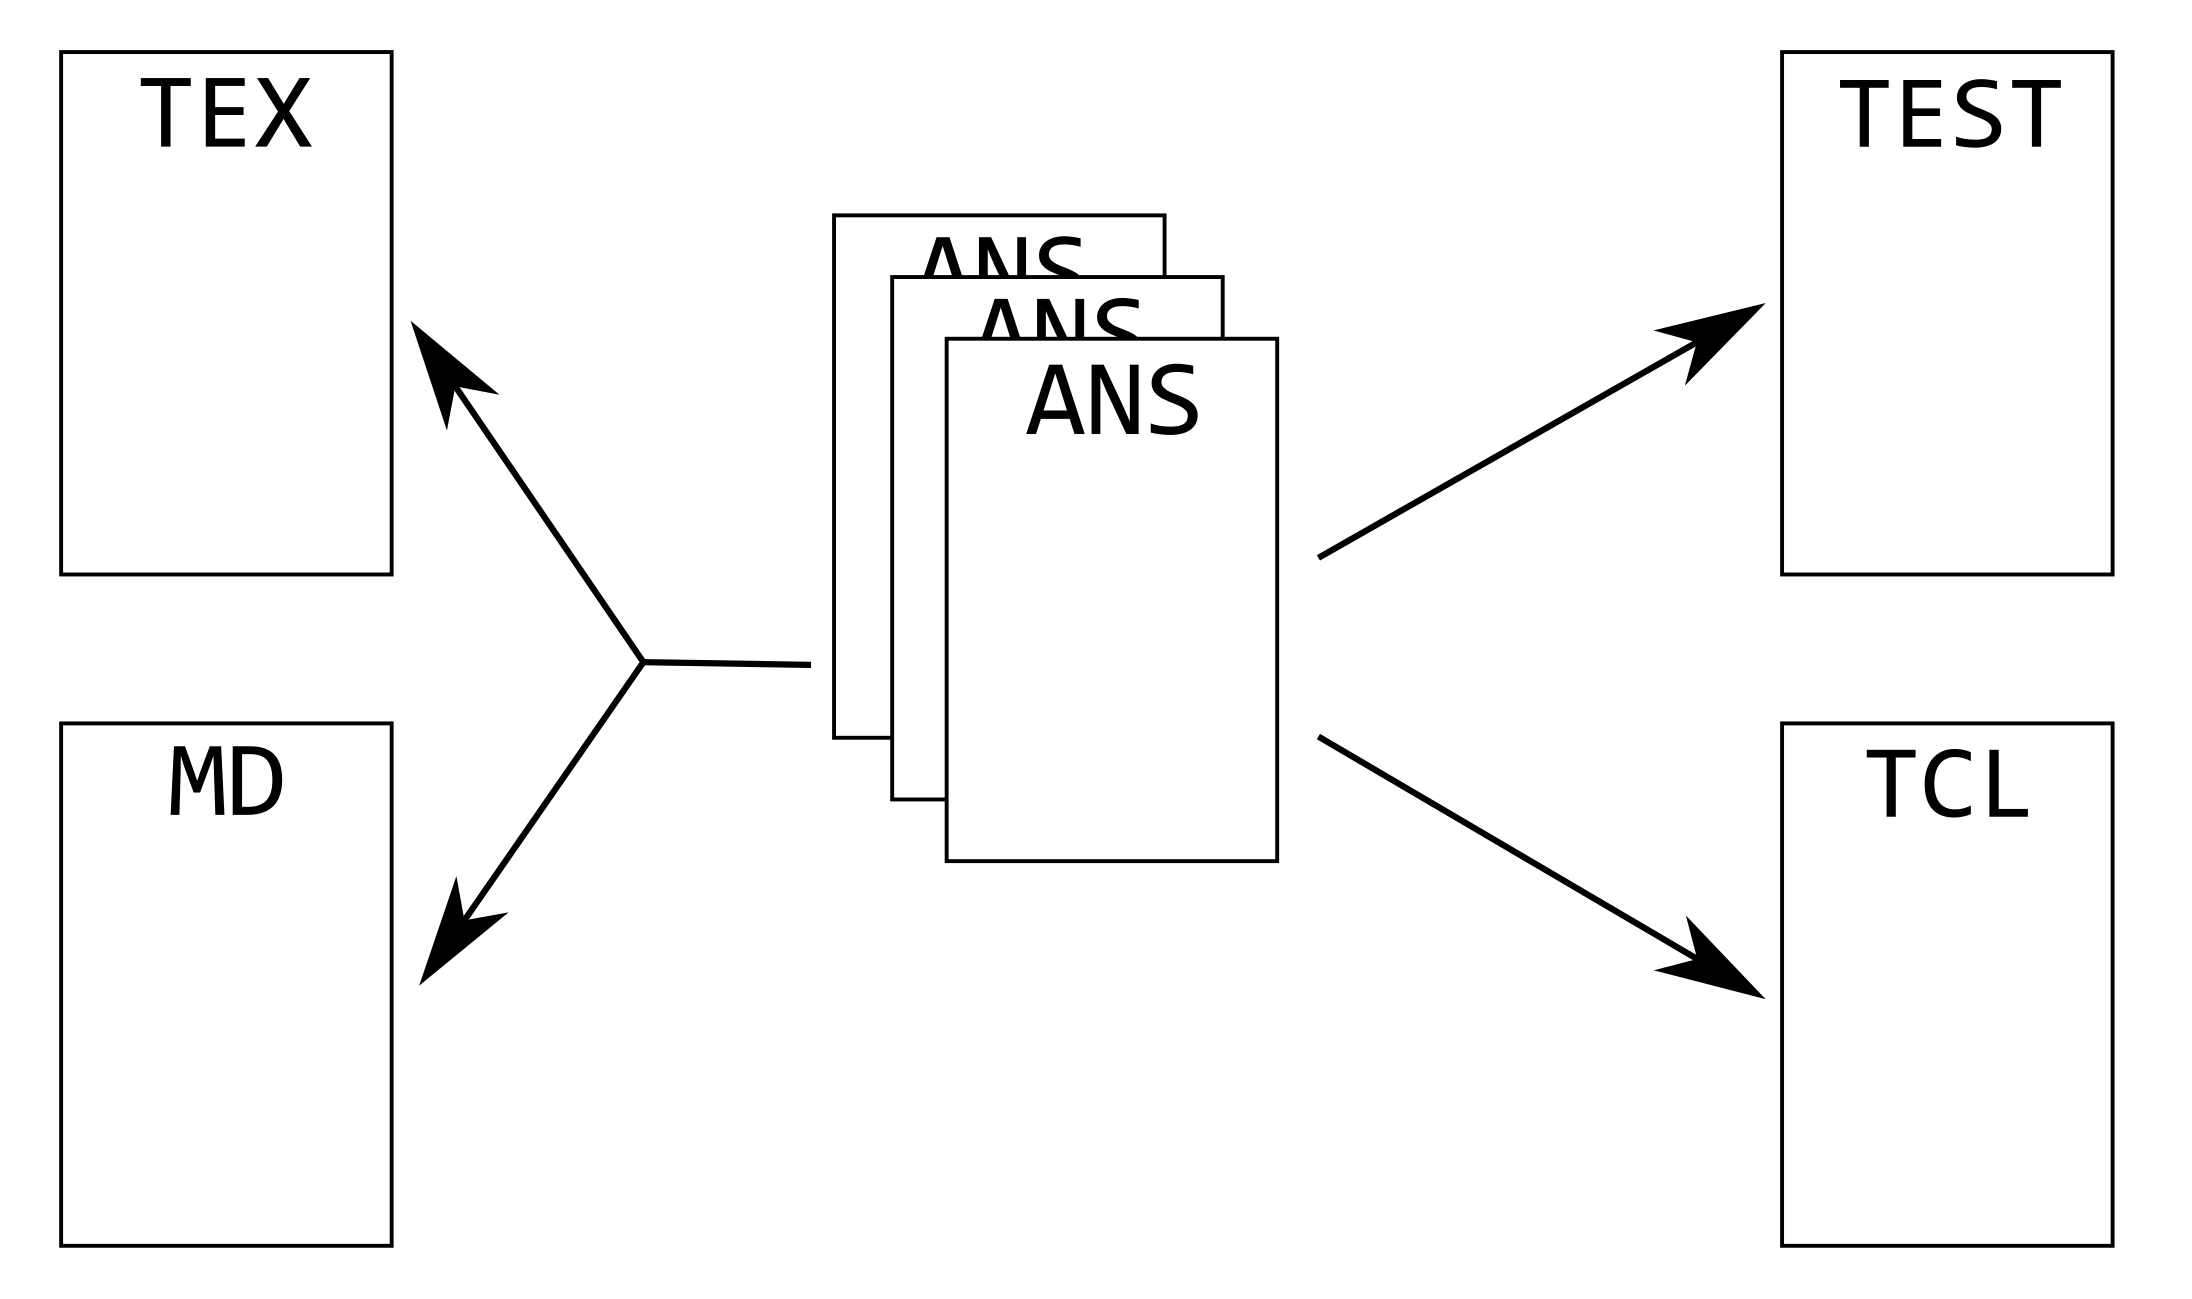
\includegraphics{images/document.png}

In the middle are a bunch of \texttt{.ans} files (ANnotated Source). These are
written with Vim. From the TT tags of those, I extract a \texttt{.test} file.
From the CB tags I extract \texttt{.tcl} source (or Scheme or C source, as the case might
be). From all the tags except TT I extract formatted documentation in Markdown
and \LaTeX{} format. All these extractions are automated using \texttt{make}.
Figures are made with Inkscape.  I create a PDF document from the \LaTeX{}
source using TeXworks. On finishing up ConsTcl, it struck me that the
documentation for this piece of software was fit for a book.

ConsTcl is at least 97\% my own work, but I have ported one part (see page
\pageref{resolving-local-defines}) from ``Scheme 9 from Empty
Space''\footnote{See \texttt{https://t3x.org/s9book/index.html}} by Nils M
Holm\index{Holm, Nils M}, a Lisp interpreter written in C and commented in a similar manner to this
book. Another source of guidance and inspiration was ``Lisp in Small Pieces'' by
Christian Queinnec.

\subsection{About the program listings}
\label{about-the-program-listings}

I have tried to write clear, readable code, but the page format forces me to
shorten lines. I have used two-space indents instead of four-space, a smaller
font, and broken off long lines with a \textbackslash\  at the end of the first
line (a so-called 'tucked-in tail'). Neither of these measures improve
readability, but the alternative is overwriting the margins. Not all broken
lines have the \textbackslash: some are broken inside a
\texttt{\{}\ldots\texttt{\}} block, and some right after a \texttt{^^5b}.

\subsection{About me}
\label{about-me}

I'm a 60 year old former system manager who has been active in programming
since 1979. Currently, since around 25 years, my language of choice is the
rather marginal Tcl\footnote{See \texttt{https://www.tcl-lang.org/}} (it's not
even in the 100 most used languages). Tcl suits me, and there are things that
one can do in Tcl that one can't easily do in other languages. Lisp is a
runner-up in my affections, a language that fascinates me but doesn't fit my
brain very well (though I have written one large piece of software in AutoLisp,
a CAD subsystem for designing drilling boxes).

In addition to my terms as programmer and system manager, I have worked as a
teacher (teaching C/C++ in upper secondary school) and for a short while I
produced textbooks for the department for information technology at
the University of Skövde. I've also been active writing answers at
question-and-answer sites on the web, mainly Stack Overflow.

\subsection{About time}
\label{about-time}

I'd like to thank

\begin{itemize}
\item my children and their lifemates for being awesome.

\item my ex-wife for supporting the printing of the book financially, and, well, for being awesome too.

\item all the wonderful people in my life for being there.
\end{itemize}

And now let's journey into the Interpreter.
\section{Unfinished code in file initial.ans line 3}
\chapter{Initial declarations}
\label{initial-declarations}
\section{Unfinished code in file initial.ans line 5}


First, I need to create the namespace that will be used for most identifiers:

\section{Unfinished code in file initial.ans line 9}
\begin{lstlisting}
namespace eval ::constcl {}
\end{lstlisting}
\section{Unfinished code in file initial.ans line 13}
\section{Utility commands}
\label{utility-commands}
\index{Utility commands}
\section{Unfinished code in file initial.ans line 15}


Next, some procedures that make my life as developer somewhat easier.

\section{Unfinished code in file initial.ans line 19}
\subsection{reg procedure}
\label{reg-procedure}
\index{reg procedure}
\section{Unfinished code in file initial.ans line 21}

\section{Unfinished code in file initial.ans line 27}

\texttt{reg} registers selected built-in procedures in the definitions register\index{definitions register}. That way I don't need to manually keep track of and list procedures. The definitions register's contents will eventually get dumped into the standard library (see page \pageref{environment-startup}). You can call \texttt{reg} with two values: \emph{key} and \emph{val}. \emph{Key} is the string that will eventually become the lookup symbol in the standard library, and \emph{val} is the name of the Tcl command that will carry out the procedure. If you don't give a value for \emph{val}, \texttt{reg} creates a value by prepending the \texttt{::constcl::} namespace to the \emph{key} value, which is sufficient 99\% of the time.

\section{Unfinished code in file initial.ans line 35}
\noindent\begin{tabular}{ |p{1.9cm} p{8cm}| }
\hline
\rowcolor[HTML]{CCCCCC} \multicolumn{2}{|l|}{\bf reg (internal)} \\
key & a Tcl string \\
?val? & a Tcl string \\
\textit{Returns:} & nothing \\
\hline
\end{tabular}
\section{Unfinished code in file initial.ans line 39}
\begin{lstlisting}
proc ::reg {key args} {
  if {[llength $args]} {
    lassign $args val
  } else {
    set val ::constcl::$key
  }
  dict set ::constcl::defreg $key $val
  return
}
\end{lstlisting}
\section{Unfinished code in file initial.ans line 51}
\subsubsection{Procedures, functions, and commands: an aside}
\label{procedures,-functions,-and-commands-an-aside}
\index{Procedures, functions, and commands: an aside}
\section{Unfinished code in file initial.ans line 53}

\section{Unfinished code in file initial.ans line 61}

I use all of these terms for the subroutines in ConsTcl. I try to stick to procedure, because that's the standard term in R5RS\footnote{Revised5 Report on the Algorithmic Language Scheme, Scheme's standardization document}. Still, they usually pass useful values back to the caller, so technically they're functions. Lastly, I'm programming in Tcl here, and the usual term for these things is `commands' in Tcl. And the `internal/public' distinction is probably a misnomer (an aside within an aside, here). What it means is that `public' procedures can be called from Lisp code being interpreted, and the others cannot. They are for use in the infrastructure around the interpreter, including in implementing the `public' procedures. Another way to put it is that procedures registered by \texttt{reg} are `public' and those who aren't are `internal'.

\section{Unfinished code in file initial.ans line 69}
\subsection{atom? procedure}
\label{atom?-procedure}
\index{atom? procedure}
\section{Unfinished code in file initial.ans line 71}

\section{Unfinished code in file initial.ans line 79}
\subsubsection{Predicates: an aside}
\label{predicates-an-aside}
\index{Predicates: an aside}
\section{Unfinished code in file initial.ans line 81}
\section{Unfinished code in file initial.ans line 86}

\texttt{THis one isn't just for my convenience: it's a standard procedure in Scheme. There are two kinds of data in Lisp: lists\index{list} and atoms\index{atom}. Lists are collections of lists and atoms. Atoms are instances of types such as booleans, characters, numbers, ports, strings, symbols, and vectors. \texttt{Atom?} recognizes an atom by checking for membership in any one of the atomic types. It returns \texttt{\#t} (truth) if it is an atom, and \texttt{\#f} (falsehood) if not. By Scheme convention, predicates\footnote{See \texttt{https://en.wikipedia.org/wiki/Boolean-valued\_function}}\index{predicate} (procedures that return either \texttt{\#t} or \texttt{\#f}) have '?' at the end of their name. Some care is necessary when calling Scheme predicates from Tcl code (the Tcl \texttt{if} command expects 1 or 0 as truth values). Example: if \{[atom? \$x]\} \ldots }

\section{Unfinished code in file initial.ans line 88}
\section{Unfinished code in file initial.ans line 90}

\texttt{will not do, but if \{[atom? \$x] ne "\#f"\} \ldots }

\section{Unfinished code in file initial.ans line 92}

(``[atom? \$x] not equal to false'') works. Or see next procedure.

\section{Unfinished code in file initial.ans line 95}
\noindent\begin{tabular}{ |p{1.9cm} p{8cm}| }
\hline
\rowcolor[HTML]{CCCCCC} \multicolumn{2}{|l|}{\bf atom? (public)} \\
val & a Lisp value \\
\textit{Returns:} & a boolean \\
\hline
\end{tabular}
\section{Unfinished code in file initial.ans line 99}
\begin{lstlisting}
reg atom? ::constcl::atom?
\section{Unfinished code in file initial.ans line 102}
proc ::constcl::atom? {val} {
  foreach type {symbol number string
      char boolean vector port eof} {
    if {[$type? $val] eq "#t"} {
      return #t
    }
  }
  return #f
}
\end{lstlisting}
\section{Unfinished code in file initial.ans line 113}
\subsection{T procedure}
\label{t-procedure}
\index{T procedure}
\section{Unfinished code in file initial.ans line 115}

\section{Unfinished code in file initial.ans line 122}

The \texttt{T} procedure is intended to reduce the hassle of trying to make Lisp booleans work with Tcl conditions. The idea is to line the Tcl condition with \texttt{[T \ldots ]} and have the Lisp expression inside \texttt{T}. \texttt{T} returns 0 if and only if the value passed to it is \texttt{\#f}, and 1 otherwise. The procedure's name stands for `truth'. Example:

\section{Unfinished code in file initial.ans line 125}
\begin{verbatim}
if {[T [atom? $x]]} ...
\end{verbatim}
\section{Unfinished code in file initial.ans line 129}
\noindent\begin{tabular}{ |p{1.9cm} p{8cm}| }
\hline
\rowcolor[HTML]{CCCCCC} \multicolumn{2}{|l|}{\bf T (internal)} \\
val & a Lisp value \\
\textit{Returns:} & a Tcl truth value (1 or 0) \\
\hline
\end{tabular}
\section{Unfinished code in file initial.ans line 133}
\begin{lstlisting}
proc ::T {val} {
  if {$val eq "#f"} {
    return 0
  } elseif {[::constcl::boolean? $val] eq "#t" &&
    [$val boolval] eq "#f"} {
    return 0
  } else {
    return 1
  }
}
\end{lstlisting}
\section{Unfinished code in file initial.ans line 146}
\subsection{assert procedure}
\label{assert-procedure}
\index{assert procedure}
\section{Unfinished code in file initial.ans line 148}


\texttt{assert} signals an error if an assertion fails.

\section{Unfinished code in file initial.ans line 152}
\noindent\begin{tabular}{ |p{1.9cm} p{8cm}| }
\hline
\rowcolor[HTML]{CCCCCC} \multicolumn{2}{|l|}{\bf assert (internal)} \\
expr &  \\
\textit{Returns:} & nothing \\
\hline
\end{tabular}
\section{Unfinished code in file initial.ans line 156}
\begin{lstlisting}
proc assert {expr} {
  if {![uplevel [list expr $expr]]} {
    error "Failed assertion [
      uplevel [list subst $expr]]"
  }
}
\end{lstlisting}
\section{Unfinished code in file initial.ans line 165}
\subsection{usage procedure}
\label{usage-procedure}
\index{usage procedure}
\section{Unfinished code in file initial.ans line 167}


\texttt{usage} is a simple procedure to compare a Lisp list (to wit: a Lisp expression) with the expected format of the expression. Mostly it just compares lengths.

\section{Unfinished code in file initial.ans line 173}
\noindent\begin{tabular}{ |p{1.9cm} p{8cm}| }
\hline
\rowcolor[HTML]{CCCCCC} \multicolumn{2}{|l|}{\bf usage (internal)} \\
usage & an expression \\
expr &  \\
none &  \\
\hline
\end{tabular}
\section{Unfinished code in file initial.ans line 177}
\begin{lstlisting}
proc ::constcl::usage {usage expr} {
  set u $usage
  set e $expr
  if {[[length $usage] numval] !=
      [[length $expr] numval]} {
    while {$u ne "#NIL" && $e ne "#NIL"} {
      set u [cdr $u]
      set e [cdr $e]
    }
    if {$e eq "#NIL" && $u ne "#NIL" &&
      [regexp {\?.*\?} [[car $u] name]]} {
      return
    }
    ::error "usage error\n[
      $usage show] not [$expr show]"
  }
}
\end{lstlisting}
\section{Unfinished code in file initial.ans line 197}
\subsection{regmacro procedure}
\label{regmacro-procedure}
\index{regmacro procedure}
\section{Unfinished code in file initial.ans line 199}


ConsTcl has macros\index{macro}, i.e. succinct syntactic forms that are rewritten to concrete--but more verbose--forms. The evaluator passes macro forms to a command for expansion before they are fully processed. \texttt{regmacro} registers macro names in the macro list, so the evaluator knows what to expand.

\section{Unfinished code in file initial.ans line 206}
\noindent\begin{tabular}{ |p{1.9cm} p{8cm}| }
\hline
\rowcolor[HTML]{CCCCCC} \multicolumn{2}{|l|}{\bf regmacro (internal)} \\
name & a Tcl string \\
\textit{Returns:} & nothing \\
\hline
\end{tabular}
\section{Unfinished code in file initial.ans line 210}
\begin{lstlisting}
proc ::regmacro {name} {
  lappend ::constcl::macrolist $name
  return
}
\end{lstlisting}
\section{Unfinished code in file initial.ans line 217}
\subsection{pn procedure}
\label{pn-procedure}
\index{pn procedure}
\section{Unfinished code in file initial.ans line 219}


\texttt{pn} stands for 'procedure name'. When called, tells the caller the name of its command. I use it for error messages so the error message can automagically tell the user which command failed.

\section{Unfinished code in file initial.ans line 225}
\noindent\begin{tabular}{ |p{1.9cm} p{8cm}| }
\hline
\rowcolor[HTML]{CCCCCC} \multicolumn{2}{|l|}{\bf pn (internal)} \\
\textit{Returns:} & a Tcl string \\
\hline
\end{tabular}
\section{Unfinished code in file initial.ans line 229}
\begin{lstlisting}
proc ::pn {} {
  lindex [split [lindex [info level -1] 0] :] end
}
\end{lstlisting}
\section{Unfinished code in file initial.ans line 235}
\subsection{typeof? procedure}
\label{typeof?-procedure}
\index{typeof? procedure}
\section{Unfinished code in file initial.ans line 237}

\section{Unfinished code in file initial.ans line 244}

\texttt{typeof?} looks at a value's type and reports if it is the same as the given type. To be certain, it looks at the value in two ways: once assuming that the value is a ConsTcl object, and once assuming that the value is an interpreter\footnote{the Tcl interpreter, not ConsTcl} alias for a ConsTcl object. If one of those affirms the type, the procedure returns \texttt{\#t}.

\section{Unfinished code in file initial.ans line 246}
\noindent\begin{tabular}{ |p{1.9cm} p{8cm}| }
\hline
\rowcolor[HTML]{CCCCCC} \multicolumn{2}{|l|}{\bf typeof? (internal)} \\
val & a Lisp value \\
type & a Tcl string \\
\textit{Returns:} & a boolean \\
\hline
\end{tabular}
\section{Unfinished code in file initial.ans line 250}
\begin{lstlisting}
proc ::constcl::typeof? {val type} {
  if {[info object isa typeof $val $type]} {
    return #t
  } elseif {[info object isa typeof \
      [interp alias {} $val] $type]} {
    return #t
  } else {
    return #f
  }
}
\end{lstlisting}
\section{Unfinished code in file initial.ans line 263}
\subsection{in-range procedure}
\label{in-range-procedure}
\index{in-range procedure}
\section{Unfinished code in file initial.ans line 265}

\section{Unfinished code in file initial.ans line 271}

This one is a little bit of both, a utility function that is also among the builtins in the library (it's not standard, though). It started out as a one-liner by Donal K. Fellows\index{Fellows, Donal}, but has grown a bit since then to suit my needs. The plan is to arrange a sequence of numbers, given one, two or three ConsTcl Number objects. If one is passed to the procedure, it is used as the end of the sequence: the sequence will end just before it. If two numbers are passed, the first one becomes the start of the sequence: the first number in it. The second number will become the end of the sequence. If three numbers are passed, they become start, end, and step, i.e. how much is added to the current number to find next number in the sequence.

\section{Unfinished code in file initial.ans line 280}
\noindent\begin{tabular}{ |p{1.9cm} p{8cm}| }
\hline
\rowcolor[HTML]{CCCCCC} \multicolumn{2}{|l|}{\bf in-range (public)} \\
x & a number \\
?e? & a number \\
?t? & a number \\
\textit{Returns:} & a Lisp list of numbers \\
\hline
\end{tabular}
\section{Unfinished code in file initial.ans line 284}
\begin{lstlisting}
reg in-range
\section{Unfinished code in file initial.ans line 287}
proc ::constcl::in-range {x args} {
  set start 0
  set step 1
  switch [llength $args] {
\section{Unfinished code in file initial.ans line 292}
      set e $x
      set end [$e numval]
    }
    1 {
      set s $x
      lassign $args e
      set start [$s numval]
      set end [$e numval]
    }
    2 {
      set s $x
      lassign $args e t
      set start [$s numval]
      set end [$e numval]
      set step [$t numval]
    }
  }
  set res $start
  while {$step > 0 && $end > [incr start $step] ||
      $step < 0 && $end < [incr start $step]} {
    lappend res $start
  }
  return [list {*}[lmap r $res {MkNumber $r}]]
}
\end{lstlisting}
\section{Unfinished code in file initial.ans line 318}
\subsection{error procedure}
\label{error-procedure}
\index{error procedure}
\section{Unfinished code in file initial.ans line 320}


\texttt{error} is used to signal an error, with \emph{msg} being a message string and the optional arguments being values to show after the message.

\section{Unfinished code in file initial.ans line 325}
\noindent\begin{tabular}{ |p{1.9cm} p{8cm}| }
\hline
\rowcolor[HTML]{CCCCCC} \multicolumn{2}{|l|}{\bf error (public)} \\
msg & a message string \\
?exprs? & some expressions \\
\textit{Returns:} & -don't care- \\
\hline
\end{tabular}
\section{Unfinished code in file initial.ans line 329}
\begin{lstlisting}
reg error
\section{Unfinished code in file initial.ans line 332}
proc ::constcl::error {msg args} {
  if {[llength $args]} {
    lappend msg "("
    set times 0
    foreach arg $args {
      if {$times} {
        ::append msg " "
      }
      ::append msg [$arg show]
      incr times
    }
    lappend msg ")"
  }
  ::error $msg
}
\end{lstlisting}
\section{Unfinished code in file initial.ans line 349}
\subsection{check procedure}
\label{check-procedure}
\index{check procedure}
\section{Unfinished code in file initial.ans line 351}


\texttt{check} does a check (typically a type check) on something and throws an error if it fails.

\section{Unfinished code in file initial.ans line 356}
\begin{lstlisting}
proc ::constcl::check {cond msg} {
  if {[uplevel $cond] eq "#f"} {
    ::error [
      uplevel [
        ::list subst [
          ::string trim $msg]]]
  }
}
\end{lstlisting}
\section{Unfinished code in file initial.ans line 367}
\section{Testing commands}
\label{testing-commands}
\index{Testing commands}
\section{Unfinished code in file initial.ans line 369}
\section{Unfinished code in file initial.ans line 373}
\subsection{pew procedure}
\label{pew-procedure}
\index{pew procedure}
\section{Unfinished code in file initial.ans line 375}


\texttt{pew} was originally named \texttt{pep} after the sequence parse-eval-print. Now it's named for parse-eval-write. It reads and evals an expression, and writes the result. It's the most common command in the test cases, since it allows me to write code directly in Scheme, get it evaled and get to see proper Lisp output from it.

\section{Unfinished code in file initial.ans line 383}
\noindent\begin{tabular}{ |p{1.9cm} p{8cm}| }
\hline
\rowcolor[HTML]{CCCCCC} \multicolumn{2}{|l|}{\bf pew (internal)} \\
str & a Tcl string, Lisp string, or a string input port \\
\textit{Returns:} & nothing \\
\hline
\end{tabular}
\section{Unfinished code in file initial.ans line 387}
\begin{lstlisting}
proc ::pew {str} {
  ::constcl::write [
    ::constcl::eval [
      ::constcl::parse $str]]
}
\end{lstlisting}
\section{Unfinished code in file initial.ans line 395}
\subsection{pw procedure}
\label{pw-procedure}
\index{pw procedure}
\section{Unfinished code in file initial.ans line 397}


\texttt{pw} is a similar command, except it doesn't eval the expression. It just writes what is parsed. It is useful for tests when the evaluator can't (yet) evaluate the form, but I can still check if it gets read and written correctly.

\section{Unfinished code in file initial.ans line 403}
\noindent\begin{tabular}{ |p{1.9cm} p{8cm}| }
\hline
\rowcolor[HTML]{CCCCCC} \multicolumn{2}{|l|}{\bf pw (internal)} \\
str & a Tcl string, Lisp string, or a string input port \\
\textit{Returns:} & nothing \\
\hline
\end{tabular}
\section{Unfinished code in file initial.ans line 407}
\begin{lstlisting}
proc ::pw {str} {
  ::constcl::write [
    ::constcl::parse $str]
}
\end{lstlisting}
\section{Unfinished code in file initial.ans line 414}
\subsection{rw procedure}
\label{rw-procedure}
\index{rw procedure}
\section{Unfinished code in file initial.ans line 416}


\texttt{rw} is the reading variant of \texttt{pw}. Instead of taking string input it takes a regular input port. The distinction mattered more while the input library was being written. The procedure just writes what is read.

\section{Unfinished code in file initial.ans line 422}
\noindent\begin{tabular}{ |p{1.9cm} p{8cm}| }
\hline
\rowcolor[HTML]{CCCCCC} \multicolumn{2}{|l|}{\bf rw (internal)} \\
?port? & an input port \\
\textit{Returns:} & nothing \\
\hline
\end{tabular}
\section{Unfinished code in file initial.ans line 426}
\begin{lstlisting}
proc ::rw {args} {
  ::constcl::write [
    ::constcl::read {*}$args]
}
\end{lstlisting}
\section{Unfinished code in file initial.ans line 433}
\subsection{pe procedure}
\label{pe-procedure}
\index{pe procedure}
\section{Unfinished code in file initial.ans line 435}


\texttt{pe} is also similar, but it doesn't write the expression. It just evaluates what is read. That way I get a value object which I can pass to another command, or pick apart in different ways.

\section{Unfinished code in file initial.ans line 441}
\noindent\begin{tabular}{ |p{1.9cm} p{8cm}| }
\hline
\rowcolor[HTML]{CCCCCC} \multicolumn{2}{|l|}{\bf pe (internal)} \\
str & a Tcl string, Lisp string, or a string input port \\
\textit{Returns:} & a Lisp value \\
\hline
\end{tabular}
\section{Unfinished code in file initial.ans line 445}
\begin{lstlisting}
proc ::pe {str} {
  ::constcl::eval [
    ::constcl::parse $str]
}
\end{lstlisting}
\section{Unfinished code in file initial.ans line 452}
\subsection{re procedure}
\label{re-procedure}
\index{re procedure}
\section{Unfinished code in file initial.ans line 454}


\texttt{re} is like \texttt{pe}, but it reads from a regular port instead of an string input port. It evaluates what is read.

\section{Unfinished code in file initial.ans line 459}
\noindent\begin{tabular}{ |p{1.9cm} p{8cm}| }
\hline
\rowcolor[HTML]{CCCCCC} \multicolumn{2}{|l|}{\bf re (internal)} \\
?port? &  \\
val &  \\
\hline
\end{tabular}
\section{Unfinished code in file initial.ans line 463}
\begin{lstlisting}
proc ::re {args} {
  ::constcl::eval [
    ::constcl::read {*}$args]
}
\end{lstlisting}
\section{Unfinished code in file initial.ans line 470}
\subsection{p procedure}
\label{p-procedure}
\index{p procedure}
\section{Unfinished code in file initial.ans line 472}


\texttt{p} only parses the input, returning an expression object.

\section{Unfinished code in file initial.ans line 476}
\noindent\begin{tabular}{ |p{1.9cm} p{8cm}| }
\hline
\rowcolor[HTML]{CCCCCC} \multicolumn{2}{|l|}{\bf p (internal)} \\
str & a Tcl string, Lisp string, or a string input port \\
\textit{Returns:} & an expression \\
\hline
\end{tabular}
\section{Unfinished code in file initial.ans line 480}
\begin{lstlisting}
proc ::p {str} {
  ::constcl::parse $str
}
\end{lstlisting}
\section{Unfinished code in file initial.ans line 486}
\subsection{e procedure}
\label{e-procedure}
\index{e procedure}
\section{Unfinished code in file initial.ans line 488}


\texttt{e} is another single-action procedure, evaluating an expression and returning a value.

\section{Unfinished code in file initial.ans line 493}
\noindent\begin{tabular}{ |p{1.9cm} p{8cm}| }
\hline
\rowcolor[HTML]{CCCCCC} \multicolumn{2}{|l|}{\bf e (internal)} \\
expr & an expression \\
\textit{Returns:} & a Lisp value \\
\hline
\end{tabular}
\section{Unfinished code in file initial.ans line 497}
\begin{lstlisting}
proc ::e {expr} {
  ::constcl::eval $expr
}
\end{lstlisting}
\section{Unfinished code in file initial.ans line 503}
\subsection{w procedure}
\label{w-procedure}
\index{w procedure}
\section{Unfinished code in file initial.ans line 505}


\texttt{w} is the third single-action procedure, printing a value and that's all.

\section{Unfinished code in file initial.ans line 509}
\noindent\begin{tabular}{ |p{1.9cm} p{8cm}| }
\hline
\rowcolor[HTML]{CCCCCC} \multicolumn{2}{|l|}{\bf w (internal)} \\
val & a Lisp value \\
\textit{Returns:} & nothing \\
\hline
\end{tabular}
\section{Unfinished code in file initial.ans line 513}
\begin{lstlisting}
proc ::w {val} {
  ::constcl::write $val
}
\end{lstlisting}
\section{Unfinished code in file initial.ans line 519}
\subsection{r procedure}
\label{r-procedure}
\index{r procedure}
\section{Unfinished code in file initial.ans line 521}


\texttt{r} is an extra single-action procedure, reading from default input or from a port and returning an expression object.

\section{Unfinished code in file initial.ans line 526}
\noindent\begin{tabular}{ |p{1.9cm} p{8cm}| }
\hline
\rowcolor[HTML]{CCCCCC} \multicolumn{2}{|l|}{\bf r (internal)} \\
?port? & an input port \\
\textit{Returns:} & an expression \\
\hline
\end{tabular}
\section{Unfinished code in file initial.ans line 530}
\begin{lstlisting}
proc ::r {args} {
  ::constcl::read {*}$args
}
\end{lstlisting}
\section{Unfinished code in file initial.ans line 536}
\subsection{prw procedure}
\label{prw-procedure}
\index{prw procedure}
\section{Unfinished code in file initial.ans line 538}


\texttt{prw} reads an expression, resolves defines, and writes the result. It was handy during the time I was porting the `resolve local defines' section.

\section{Unfinished code in file initial.ans line 543}
\noindent\begin{tabular}{ |p{1.9cm} p{8cm}| }
\hline
\rowcolor[HTML]{CCCCCC} \multicolumn{2}{|l|}{\bf prw (internal)} \\
str & a Tcl string, Lisp string, or a string input port \\
\textit{Returns:} & nothing \\
\hline
\end{tabular}
\section{Unfinished code in file initial.ans line 547}
\begin{lstlisting}
proc ::prw {str} {
  set expr [::constcl::parse $str]
  set expr [::constcl::resolve-local-defines \
    [::constcl::cdr $expr]]
  ::constcl::write $expr
}
\end{lstlisting}
\section{Unfinished code in file initial.ans line 556}
\subsection{pxw procedure}
\label{pxw-procedure}
\index{pxw procedure}
\section{Unfinished code in file initial.ans line 558}


\texttt{pxw} attempts to macro-expand whatever it reads, and writes the result. I know that 'expand' doesn't start with an 'x'. Again, this command's heyday was when I was developing the macro facility.

\section{Unfinished code in file initial.ans line 564}
\noindent\begin{tabular}{ |p{1.9cm} p{8cm}| }
\hline
\rowcolor[HTML]{CCCCCC} \multicolumn{2}{|l|}{\bf pxw (internal)} \\
str & a Tcl string, Lisp string, or a string input port \\
\textit{Returns:} & nothing \\
\hline
\end{tabular}
\section{Unfinished code in file initial.ans line 568}
\begin{lstlisting}
proc ::pxw {str} {
  set expr [::constcl::parse $str]
  set expr [::constcl::expand-macro $expr \
    ::constcl::global_env]
  ::constcl::write $expr
}
\end{lstlisting}
\section{Unfinished code in file initial.ans line 577}
\section{Some small classes}
\label{some-small-classes}
\index{Some small classes}
\section{Unfinished code in file initial.ans line 579}
\subsection{Dot class}
\label{dot-class}
\index{Dot class}
\section{Unfinished code in file initial.ans line 581}


The \texttt{Dot} class is a helper class for the parser.

\section{Unfinished code in file initial.ans line 585}
\begin{lstlisting}
catch { ::constcl::Dot destroy }
\section{Unfinished code in file initial.ans line 588}
oo::class create ::constcl::Dot {
  method mkconstant {} {}
  method write {handle} {
    puts -nonewline $handle "."
  }
  method display {handle} {
    my write $handle
  }
}
\end{lstlisting}
\section{Unfinished code in file initial.ans line 599}
\subsection{dot? procedure}
\label{dot?-procedure}
\index{dot? procedure}
\section{Unfinished code in file initial.ans line 601}


\texttt{dot?} is a type predicate that checks for membership in the type \texttt{Dot}.

\section{Unfinished code in file initial.ans line 605}
\noindent\begin{tabular}{ |p{1.9cm} p{8cm}| }
\hline
\rowcolor[HTML]{CCCCCC} \multicolumn{2}{|l|}{\bf dot? (internal)} \\
val & a Lisp value \\
\textit{Returns:} & a boolean \\
\hline
\end{tabular}
\section{Unfinished code in file initial.ans line 609}
\begin{lstlisting}
proc ::constcl::dot? {val} {
  typeof? $val "Dot"
}
\end{lstlisting}
\section{Unfinished code in file initial.ans line 615}
\subsection{EndOfFile class}
\label{endoffile-class}
\index{EndOfFile class}
\section{Unfinished code in file initial.ans line 617}


The \texttt{EndOfFile} class is for end-of-file\index{end of file} conditions.

\section{Unfinished code in file initial.ans line 621}
\begin{lstlisting}
catch { ::constcl::EndOfFile destroy }
\section{Unfinished code in file initial.ans line 624}
oo::singleton create ::constcl::EndOfFile {
  method mkconstant {} {}
  method write {handle} {
    puts -nonewline $handle "#<end-of-file>"
  }
  method display {handle} {
    my write $handle
  }
}
\end{lstlisting}
\section{Unfinished code in file initial.ans line 635}
\subsection{eof? procedure}
\label{eof?-procedure}
\index{eof? procedure}
\section{Unfinished code in file initial.ans line 637}


\texttt{eof?} is a type predicate that recognizes the end-of-file object.

\section{Unfinished code in file initial.ans line 641}
\noindent\begin{tabular}{ |p{1.9cm} p{8cm}| }
\hline
\rowcolor[HTML]{CCCCCC} \multicolumn{2}{|l|}{\bf eof? (internal)} \\
val & a Lisp value \\
\textit{Returns:} & a boolean \\
\hline
\end{tabular}
\section{Unfinished code in file initial.ans line 645}
\begin{lstlisting}
proc eof? {val} {
  if {$val eq "#EOF"} {
    return #t
  } else {
    return #f
  }
}
\end{lstlisting}
\section{Unfinished code in file initial.ans line 655}
\subsection{NIL class}
\label{nil-class}
\index{NIL class}
\section{Unfinished code in file initial.ans line 657}


The \texttt{NIL} class has one object: the empty list called \texttt{\#NIL}. It is also base class for many other type classes.

\section{Unfinished code in file initial.ans line 662}
\begin{lstlisting}
catch { ::constcl::NIL destroy }
\section{Unfinished code in file initial.ans line 665}
oo::singleton create ::constcl::NIL {
  method boolval {} {
    return #t
  }
  method car {} {
    ::error "PAIR expected"
  }
  method cdr {} {
    ::error "PAIR expected"
  }
  method set-car! {v} {
    ::error "PAIR expected"
  }
  method set-cdr! {v} {
    ::error "PAIR expected"
  }
  method numval {} {
    ::error "NUMBER expected"
  }
  method write {handle} {
    puts -nonewline $handle "()"
  }
  method display {handle} {
    my write $handle
  }
  method show {} {
    format "()"
  }
}
\end{lstlisting}
\section{Unfinished code in file initial.ans line 696}
\subsection{null? procedure}
\label{null?-procedure}
\index{null? procedure}
\section{Unfinished code in file initial.ans line 698}


The \texttt{null?} standard predicate recognizes the empty list.

\section{Unfinished code in file initial.ans line 702}
\noindent\begin{tabular}{ |p{1.9cm} p{8cm}| }
\hline
\rowcolor[HTML]{CCCCCC} \multicolumn{2}{|l|}{\bf null? (public)} \\
val & a Lisp value \\
\textit{Returns:} & a boolean \\
\hline
\end{tabular}
\section{Unfinished code in file initial.ans line 706}
\begin{lstlisting}
reg null?
\section{Unfinished code in file initial.ans line 709}
proc ::constcl::null? {val} {
  if {$val eq "#NIL"} {
    return #t
  } else {
    return #f
  }
}
\end{lstlisting}
\section{Unfinished code in file initial.ans line 718}
\subsection{Undefined class}
\label{undefined-class}
\index{Undefined class}
\section{Unfinished code in file initial.ans line 720}


The \texttt{Undefined} class is for undefined things. It was created to facilitate porting of code from `Scheme 9 from Empty Space'\index{S9fES}.

\section{Unfinished code in file initial.ans line 725}
\begin{lstlisting}
catch { ::constcl::Undefined destroy }
\section{Unfinished code in file initial.ans line 728}
oo::class create ::constcl::Undefined {
  method mkconstant {} {}
  method write {handle} {
    puts -nonewline $handle "#<undefined>"
  }
  method display {handle} {
    my write $handle
  }
}
\end{lstlisting}
\section{Unfinished code in file initial.ans line 739}
\subsection{Unspecified class}
\label{unspecified-class}
\index{Unspecified class}
\section{Unfinished code in file initial.ans line 741}


The \texttt{Unspecified} class is for unspecified things. Also a S9fES support class.

\section{Unfinished code in file initial.ans line 745}
\begin{lstlisting}
catch { ::constcl::Unspecified destroy }
\section{Unfinished code in file initial.ans line 748}
oo::class create ::constcl::Unspecified {
  method mkconstant {} {}
  method write {handle} {
    puts -nonewline $handle "#<unspecified>"
  }
  method display {handle} {
    my write $handle
  }
}
\end{lstlisting}
\section{Unfinished code in file initial.ans line 759}
\section{Unfinished code in file initial.ans line 761}
\section{Unfinished code in file input.ans line 3}
\chapter{Input}
\label{input}
\section{Unfinished code in file input.ans line 5}

\section{Unfinished code in file input.ans line 11}

The first thing an interpreter must be able to do is to take in the user's code and data input\index{input}, whether from the keyboard or from a source file. \texttt{read} represents the interpreter's main input facility. The \texttt{read-} procedures read from standard input, or--if a port is provided--from the port's channel. The main input procedures, \texttt{read} and the non-standard \texttt{parse}, do more than just read in the text of code and data: they also \emph{parse} the input into an \emph{internal representation} that the evaluator can use.

\section{Unfinished code in file input.ans line 16}
\section{The parsing process}
\label{the-parsing-process}
\index{The parsing process}
\section{Unfinished code in file input.ans line 18}

\section{Unfinished code in file input.ans line 24}
\section{Unfinished code in file input.ans line 28}
\section{Unfinished code in file input.ans line 36}
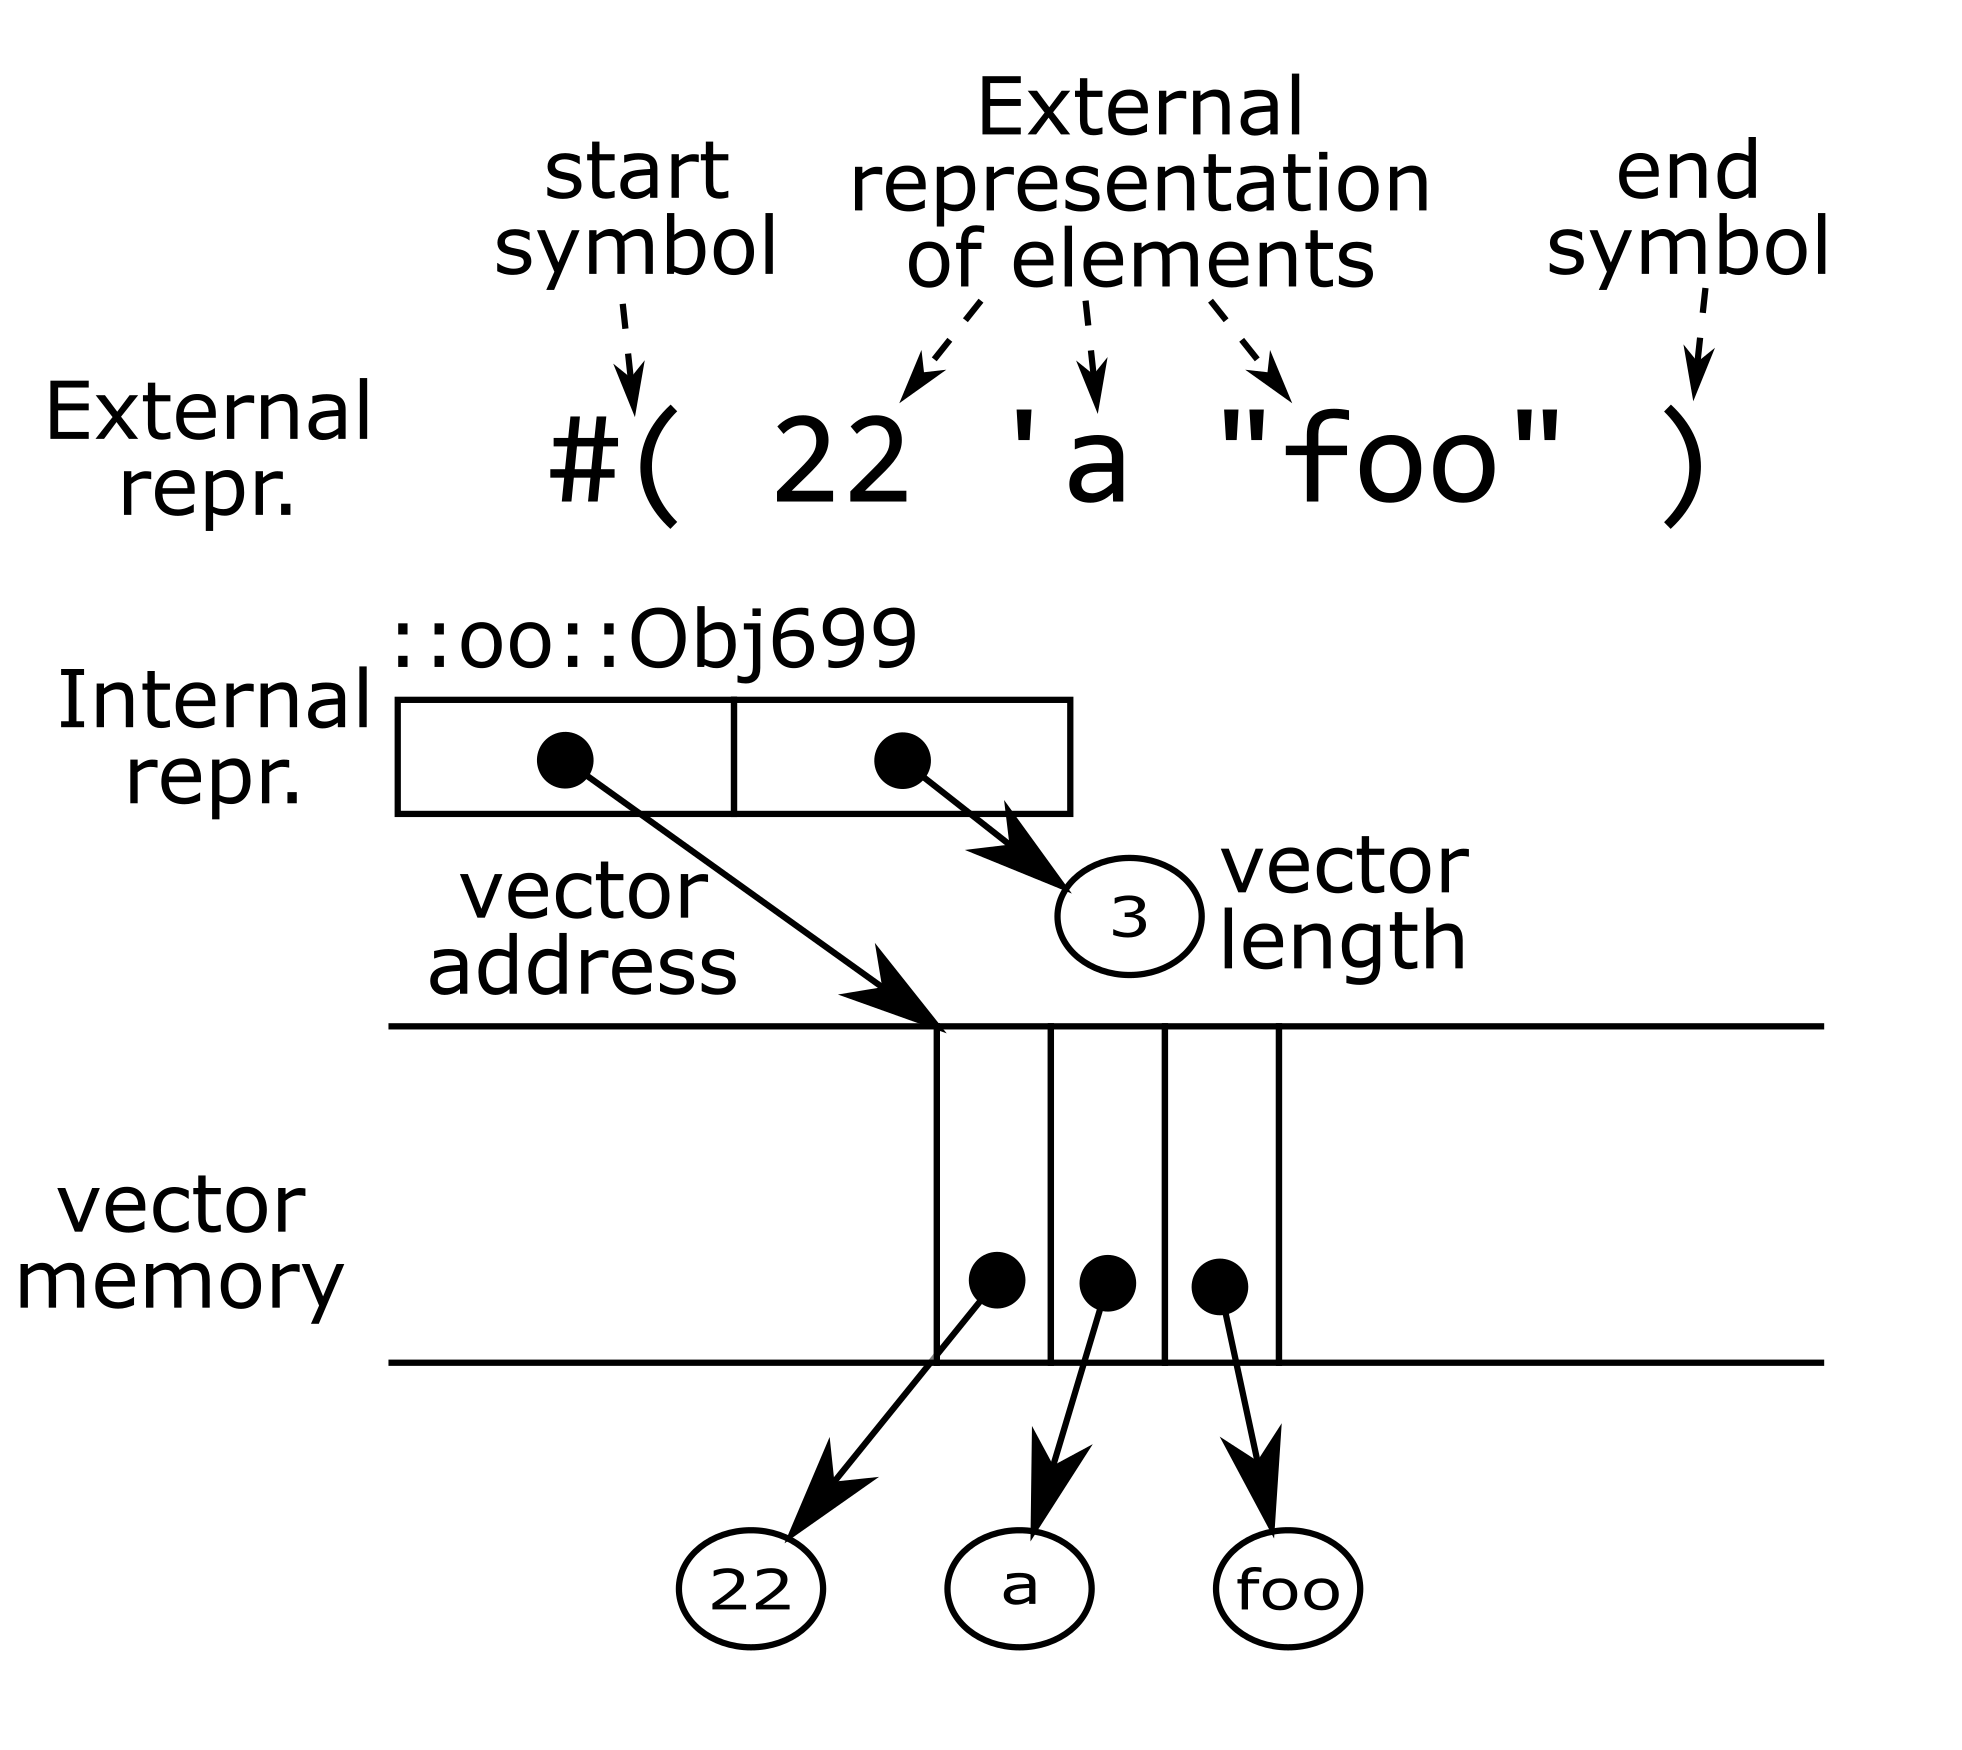
\includegraphics{images/vector-representation.png}
\section{Unfinished code in file input.ans line 38}
\section{Unfinished code in file input.ans line 43}
\section{Unfinished code in file input.ans line 46}

Parsing\footnote{See \texttt{https://en.wikipedia.org/wiki/Parsing}}\index{parsing}, or syntactic analysis, is analyzing a sequence of letters, digits, and other characters, conforming to the rules of \emph{external representation}\index{external representation}. The result of parsing is an \emph{expression}\index{expression}. The parsing process translates a piece of text from external representation to internal representation. The external representation is a 'recipe' for an expression that expresses it in a unique way. For example, the external representation for a vector is a pound sign (\texttt{\#}), a left parenthesis (\texttt{(}), the external representation for some values, and a right parenthesis (\texttt{)}). When the reader or parser is working through input, a \texttt{\#(} symbol signals that a vector structure is being read. A number of subexpressions for the elements of the vector follow, and then a closing parenthesis \texttt{)} signals that the vector is done. The elements are saved in vector memory and the vector gets the address to the first element and the number of elements. The \texttt{parse} or \texttt{read} procedure takes in the input buffer character by character, matching each character against a fitting external representation. When done, it creates a ConsTcl object, which is the internal representation of an expression. The object can then be passed to the evaluator. Given a string, \texttt{parse} creates a string input port for itself to read from. It then parses the input and produces the internal representation of an expression. Example:

\section{Unfinished code in file input.ans line 49}
\begin{verbatim}
% ::constcl::parse "(+ 2 3)"
::oo::Obj491
\end{verbatim}
\section{Unfinished code in file input.ans line 54}


Here, \texttt{parse} parsed the external representation of a list with three elements, +, 2, and 3. It produced the expression that has an internal representation labeled \texttt{::oo::Obj491}. I will now reach briefly into the following chapters and present procedures like \texttt{eval}, which transforms an expression into a value, and \texttt{write}, which writes a printed external representation of expressions and values. Putting them together we can see

\section{Unfinished code in file input.ans line 63}
\begin{verbatim}
% ::constcl::write ::oo::Obj491
(+ 2 3)
% ::constcl::eval ::oo::Obj491
::oo::Obj494
% ::constcl::write ::oo::Obj494
5
\end{verbatim}
\section{Unfinished code in file input.ans line 72}


Fortunately, we don't \emph{have} to work at such a low level. We can use the \texttt{repl}\index{repl} instead:

\section{Unfinished code in file input.ans line 77}
\begin{verbatim}
ConsTcl> (+ 2 3)
5
\end{verbatim}
\section{Unfinished code in file input.ans line 82}

\section{Unfinished code in file input.ans line 86}

Then, parsing and evaluation and writing goes on in the background and the internal representations of expressions and values are hidden. Anyway, the figure shows is what it really looks like. \texttt{::oo::Obj491} was just the head of the list.

\section{Unfinished code in file input.ans line 90}
\begin{figure}[h!]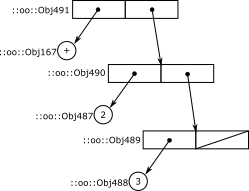
\includegraphics{images/intreplist.png}\captionsetup{labelformat=empty}\caption{ The internal structure of the expression}\label{fig:-the-internal-structure-of-the-expression}\end{figure}
\section{Unfinished code in file input.ans line 92}
\section{Input procedures}
\label{input-procedures}
\index{Input procedures}
\section{Unfinished code in file input.ans line 94}
\subsubsection{Ports: an aside}
\label{ports-an-aside}
\index{Ports: an aside}
\section{Unfinished code in file input.ans line 96}


Ports are an abstraction of the input or output mechanism. An input port can be connected to standard input (the keyboard\footnote{which doesn't work in a Windows windowing environment, i.e. wish or tkcon. repl does work, though.}) or a file opened for input or (a ConsTcl extension) a string input buffer where the complete available input is laid out before reading starts. Regardless of what kind of input port it is, one can read characters from it until it runs out and signals end-of-file. Likewise, an output port, regardless of whether it's the standard output--the screen--or a file opened for output, will receive characters sent to it.

\section{Unfinished code in file input.ans line 108}
\subsection{parse procedure}
\label{parse-procedure}
\index{parse procedure}
\section{Unfinished code in file input.ans line 110}


\texttt{parse} can be called with either a string input port or a Tcl or ConsTcl string (which it uses to open a string input port). Once the input port is established, \texttt{parse} leaves control to \texttt{read-expr} (see page \pageref{read-expr-procedure}).

\section{Unfinished code in file input.ans line 116}
\noindent\begin{tabular}{ |p{1.9cm} p{8cm}| }
\hline
\rowcolor[HTML]{CCCCCC} \multicolumn{2}{|l|}{\bf parse (internal)} \\
inp & a Tcl string, Lisp string, or a string input port \\
\textit{Returns:} & an expression \\
\hline
\end{tabular}
\section{Unfinished code in file input.ans line 120}
\begin{lstlisting}
reg parse
\section{Unfinished code in file input.ans line 123}
proc ::constcl::parse {inp} {
  set c {}
  set unget {}
  if {[info object isa object $inp]} {
    if {[T [typeof? $inp StringInputPort]]} {
      set port $inp
    } elseif {[T [typeof? $inp String]]} {
      set port [StringInputPort new [$inp value]]
    } else {
      ::error "Unknown object [$inp show]"
    }
  } else {
    # It's a Tcl string, we hope
    set port [StringInputPort new $inp]
  }
  set oldport $::constcl::Input_port
  set ::constcl::Input_port $port
  set expr [read-expr]
  set ::constcl::Input_port $oldport
  return $expr
}
\end{lstlisting}
\section{Unfinished code in file input.ans line 146}
\section{Unfinished code in file input.ans line 151}
\section{Unfinished code in file input.ans line 155}
\section{Unfinished code in file input.ans line 160}
\subsection{read procedure}
\label{read-procedure}
\index{read procedure}
\section{Unfinished code in file input.ans line 162}

\section{Unfinished code in file input.ans line 167}

The standard builtin \texttt{read} reads an input port the same way that \texttt{parse} does, but one can't pass a string to it. The \texttt{read-} procedures parse their input and produce ConsTcl objects. One can pass a port to \texttt{read} (including a string input port) in which case \texttt{read} sets the standard input port temporarily to the provided port. If not, \texttt{read} uses the default standard input port (usually the keyboard\footnote{which, again, doesn't work in a Windows windowing application.}).

\section{Unfinished code in file input.ans line 173}
\noindent\begin{tabular}{ |p{1.9cm} p{8cm}| }
\hline
\rowcolor[HTML]{CCCCCC} \multicolumn{2}{|l|}{\bf read (public)} \\
?port? & a port \\
\textit{Returns:} & an expression \\
\hline
\end{tabular}
\section{Unfinished code in file input.ans line 177}
\begin{lstlisting}
reg read
\section{Unfinished code in file input.ans line 180}
proc ::constcl::read {args} {
  set c {}
  set unget {}
  if {[llength $args]} {
    lassign $args port
  } else {
    set port $::constcl::Input_port
  }
  set oldport $::constcl::Input_port
  set ::constcl::Input_port $port
  set expr [read-expr]
  set ::constcl::Input_port $oldport
  return $expr
}
\end{lstlisting}
\section{Unfinished code in file input.ans line 196}
\section{Unfinished code in file input.ans line 200}
\section{Input helper procedures}
\label{input-helper-procedures}
\index{Input helper procedures}
\section{Unfinished code in file input.ans line 202}
\subsection{make-constant procedure}
\label{make-constant-procedure}
\index{make-constant procedure}
\section{Unfinished code in file input.ans line 204}


The \texttt{make-constant} helper procedure is called to set expressions to constants when read as a literal.

\section{Unfinished code in file input.ans line 209}
\begin{lstlisting}
proc ::constcl::make-constant {val} {
  if {[T [pair? $val]]} {
    $val mkconstant
    make-constant [car $val]
    make-constant [cdr $val]
  } elseif {[T [null? $val]]} {
    return #NIL
  } else {
    $val mkconstant
  }
}
\end{lstlisting}
\section{Unfinished code in file input.ans line 223}
\section{Unfinished code in file input.ans line 227}
\subsection{interspace? procedure}
\label{interspace?-procedure}
\index{interspace? procedure}
\section{Unfinished code in file input.ans line 229}


The \texttt{interspace?} helper procedure recognizes whitespace between value representations.

\section{Unfinished code in file input.ans line 234}
\begin{lstlisting}
proc ::constcl::interspace? {c} {
  if {[::string is space $c] || $c eq ";"} {
      return #t
    } else {
      return #f
    }
}
\end{lstlisting}
\section{Unfinished code in file input.ans line 244}
\section{Unfinished code in file input.ans line 248}
\subsection{valid-char? procedure}
\label{valid-char?-procedure}
\index{valid-char? procedure}
\section{Unfinished code in file input.ans line 250}


The \texttt{valid-char?} helper procedure compares a potential character constant to the valid kinds.

\section{Unfinished code in file input.ans line 255}
\noindent\begin{tabular}{ |p{1.9cm} p{8cm}| }
\hline
\rowcolor[HTML]{CCCCCC} \multicolumn{2}{|l|}{\bf valid-char? (internal)} \\
name & a Tcl string \\
\textit{Returns:} & a boolean \\
\hline
\end{tabular}
\section{Unfinished code in file input.ans line 259}
\begin{lstlisting}
proc ::constcl::valid-char? {name} {
  if {[regexp {(?i)^#\\([[:graph:]]|space|newline)$} \
      $name]} {
    return #t
  } else {
    return #f
  }
}
\end{lstlisting}
\section{Unfinished code in file input.ans line 270}
\section{Unfinished code in file input.ans line 274}
\subsection{readc procedure}
\label{readc-procedure}
\index{readc procedure}
\section{Unfinished code in file input.ans line 276}


\texttt{readc} reads one character from the unget store if it isn't empty or else from the input port. If the input is at end-of-file, an eof object is returned. Shares the variable \texttt{unget} with its caller.

\section{Unfinished code in file input.ans line 282}
\noindent\begin{tabular}{ |p{1.9cm} p{8cm}| }
\hline
\rowcolor[HTML]{CCCCCC} \multicolumn{2}{|l|}{\bf readc (internal)} \\
\textit{Returns:} & a Tcl character or end of file \\
\hline
\end{tabular}
\section{Unfinished code in file input.ans line 286}
\begin{lstlisting}
proc ::constcl::readc {} {
  upvar unget unget
  if {$unget ne {}} {
    set c $unget
    set unget {}
  } else {
    set c [$::constcl::Input_port get]
    if {[$::constcl::Input_port eof]} {
      return #EOF
    }
  }
  return $c
}
\end{lstlisting}
\section{Unfinished code in file input.ans line 302}
\section{Unfinished code in file input.ans line 306}
\subsection{find-char? procedure}
\label{find-char?-procedure}
\index{find-char? procedure}
\section{Unfinished code in file input.ans line 308}


\texttt{find-char?} reads ahead through whitespace to find a given character. It returns \texttt{\#t} if it has found the character, and \texttt{\#f} if it has stopped at some other character. Returns end of file if eof is encountered. Shares the variables \texttt{c} and \texttt{unget} with its caller.

\section{Unfinished code in file input.ans line 315}
\noindent\begin{tabular}{ |p{1.9cm} p{8cm}| }
\hline
\rowcolor[HTML]{CCCCCC} \multicolumn{2}{|l|}{\bf find-char? (internal)} \\
char & a Tcl character \\
\textit{Returns:} & a boolean or end of file \\
\hline
\end{tabular}
\section{Unfinished code in file input.ans line 319}
\begin{lstlisting}
proc ::constcl::find-char? {char} {
  upvar c c unget unget
  while {[::string is space -strict $c]} {
    set c [readc]
    read-eof $c
    set unget $c
  }
  expr {($c eq $char) ? "#t" : "#f"}
}
\end{lstlisting}
\section{Unfinished code in file input.ans line 331}
\section{Unfinished code in file input.ans line 335}
\subsection{read-end? procedure}
\label{read-end?-procedure}
\index{read-end? procedure}
\section{Unfinished code in file input.ans line 337}


\texttt{read-end?} reads one character and returns \texttt{\#t} if it is an interspace character or an ending parenthesis or bracket, or end of file. Otherwise it returns \texttt{\#f}. It ungets the character before returning. Shares the variables \texttt{c} and \texttt{unget} with its caller.

\section{Unfinished code in file input.ans line 344}
\noindent\begin{tabular}{ |p{1.9cm} p{8cm}| }
\hline
\rowcolor[HTML]{CCCCCC} \multicolumn{2}{|l|}{\bf read-end? (internal)} \\
\textit{Returns:} & a boolean or end of file \\
\hline
\end{tabular}
\section{Unfinished code in file input.ans line 348}
\begin{lstlisting}
proc ::constcl::read-end? {} {
  upvar c c unget unget
  set c [readc]
  if {[T [interspace? $c]] || $c in {) ]} || $c eq "#EOF"} {
    set unget $c
    return #t
  } else {
    set unget $c
    return #f
  }
}
\end{lstlisting}
\section{Unfinished code in file input.ans line 362}
\section{Unfinished code in file input.ans line 366}
\subsection{skip-ws procedure}
\label{skip-ws-procedure}
\index{skip-ws procedure}
\section{Unfinished code in file input.ans line 368}


\texttt{skip-ws} skips whitespace and comments (the \texttt{;} to end of line kind). It leaves the first character not to be skipped in \texttt{c} and also ungets it. Shares the variables \texttt{c} and \texttt{unget} with its caller.

\section{Unfinished code in file input.ans line 373}
\noindent\begin{tabular}{ |p{1.9cm} p{8cm}| }
\hline
\rowcolor[HTML]{CCCCCC} \multicolumn{2}{|l|}{\bf skip-ws (internal)} \\
\textit{Returns:} & nothing \\
\hline
\end{tabular}
\section{Unfinished code in file input.ans line 377}
\begin{lstlisting}
proc ::constcl::skip-ws {} {
  upvar c c unget unget
  while true {
    switch -regexp $c {
      {[[:space:]]} {
        set c [readc]
      }
      {;} {
        while {$c ne "\n" && $c ne "#EOF"}  {
          set c [readc]
        }
      }
      default {
        set unget $c
        return
      }
    }
  }
}
\end{lstlisting}
\section{Unfinished code in file input.ans line 399}
\section{Unfinished code in file input.ans line 403}
\subsection{read-eof procedure}
\label{read-eof-procedure}
\index{read-eof procedure}
\section{Unfinished code in file input.ans line 405}


\texttt{read-eof} checks a number of presumed characters for possible end-of-file objects. If it finds one, it returns \emph{from its caller} with the EOF value.

\section{Unfinished code in file input.ans line 410}
\noindent\begin{tabular}{ |p{1.9cm} p{8cm}| }
\hline
\rowcolor[HTML]{CCCCCC} \multicolumn{2}{|l|}{\bf read-eof (internal)} \\
chars & some characters \\
\hline
\end{tabular}
\section{Unfinished code in file input.ans line 414}
\begin{lstlisting}
proc ::constcl::read-eof {args} {
  set chars $args
  foreach char $chars {
    if {$char eq "#EOF"} {
      return -level 1 -code return #EOF
    }
  }
}
\end{lstlisting}
\section{Unfinished code in file input.ans line 425}
\section{Unfinished code in file input.ans line 429}
\section{Reader procedures}
\label{reader-procedures}
\index{Reader procedures}
\section{Unfinished code in file input.ans line 431}


Reader procedures specialize in reading a certain kind of input, except for \texttt{read-expr} which reads them all (with a little help).

\section{Unfinished code in file input.ans line 436}
\subsection{read-expr procedure}
\label{read-expr-procedure}
\index{read-expr procedure}
\section{Unfinished code in file input.ans line 438}


The \texttt{read-expr} procedure reads the first available character from the input port. Based on that it delegates to one of the more detailed readers, producing an expression of any kind. A Tcl character value can be passed to it: that character will be used first before reading from the input. If end of file is encountered before an expression can be read in full, the procedure returns end of file (\texttt{\#EOF})\index{end of file}. Shares the variables \texttt{c} and \texttt{unget} with its caller.

\section{Unfinished code in file input.ans line 448}
\noindent\begin{tabular}{ |p{1.9cm} p{8cm}| }
\hline
\rowcolor[HTML]{CCCCCC} \multicolumn{2}{|l|}{\bf read-expr (internal)} \\
?char? & a Tcl character \\
\textit{Returns:} & an expression or end of file \\
\hline
\end{tabular}
\section{Unfinished code in file input.ans line 452}
\begin{lstlisting}
proc ::constcl::read-expr {args} {
  upvar c c unget unget
  if {[llength $args]} {
    lassign $args c
  } else {
    set c [readc]
  }
  set unget {}
  read-eof $c
  if {[::string is space $c] || $c eq ";"} {
    skip-ws
    read-eof $c
  }
  switch -regexp $c {
    {\"}          { read-string-expr }
    {\#}          { read-pound }
    {\'}          { read-quoted-expr }
    {\(}          { read-pair-expr ")" }
    {\+} - {\-}   { read-plus-minus $c }
    {\,}          { read-unquoted-expr }
    {\.} {
        set x [Dot new]; set c [readc]; set x
    }
    {\:}          { read-object-expr }
    {\[}          { read-pair-expr "\]" }
    {\`}          { read-quasiquoted-expr }
    {\d}          { read-number-expr $c }
    {^$}          { return }
    {[[:graph:]]} { read-identifier-expr $c }
    default {
      read-eof $c
      ::error "unexpected character ($c)"
    }
  }
}
\end{lstlisting}
\section{Unfinished code in file input.ans line 490}
\section{Unfinished code in file input.ans line 503}
\section{Unfinished code in file input.ans line 505}
\subsection{read-character-expr procedure}
\label{read-character-expr-procedure}
\index{read-character-expr procedure}
\section{Unfinished code in file input.ans line 507}


\texttt{read-character-expr} is activated by \texttt{read-pound} when that procedure finds a backslash in the input stream (pound-backslash is the external representation prefix for characters). It reads one or more characters to produce a character expression and return a Char (see page \pageref{characters}) object. Shares the variables \texttt{c} and \texttt{unget} with its caller.

\section{Unfinished code in file input.ans line 515}
\noindent\begin{tabular}{ |p{1.9cm} p{8cm}| }
\hline
\rowcolor[HTML]{CCCCCC} \multicolumn{2}{|l|}{\bf read-character-expr (internal)} \\
\textit{Returns:} & a character or end of file \\
\hline
\end{tabular}
\section{Unfinished code in file input.ans line 519}
\begin{lstlisting}
proc ::constcl::read-character-expr {} {
  upvar c c unget unget
  set name "#\\"
  set c [readc]
  read-eof $c
  while {$c ni {) ]} && [::string is graph $c] && $c ne "#EOF"} {
    ::append name $c
    set c [readc]
  }
  check {valid-char? $name} {
      Invalid character constant $name
  }
  set expr [MkChar $name]
  read-eof $expr
  return $expr
}
\end{lstlisting}
\section{Unfinished code in file input.ans line 538}
\section{Unfinished code in file input.ans line 540}
\section{Unfinished code in file input.ans line 546}
\section{Unfinished code in file input.ans line 551}
\section{Unfinished code in file input.ans line 562}
\section{Unfinished code in file input.ans line 564}
\subsection{read-identifier-expr procedure}
\label{read-identifier-expr-procedure}
\index{read-identifier-expr procedure}
\section{Unfinished code in file input.ans line 566}


\texttt{read-identifier-expr} is activated for 'anything else', and takes in characters until it finds whitespace or an ending parenthesis or bracket. If it is passed one or more characters it will use them before consuming any from input. It checks the input against the rules for identifiers, accepting or rejecting it with an error message. It returns a Symbol (see page \pageref{symbols}) object. Shares the variables \texttt{c} and \texttt{unget} with its caller.

\section{Unfinished code in file input.ans line 575}
\noindent\begin{tabular}{ |p{1.9cm} p{8cm}| }
\hline
\rowcolor[HTML]{CCCCCC} \multicolumn{2}{|l|}{\bf read-identifier-expr (internal)} \\
?chars? & some Tcl characters \\
\textit{Returns:} & a symbol or end of file \\
\hline
\end{tabular}
\section{Unfinished code in file input.ans line 579}
\begin{lstlisting}
proc ::constcl::read-identifier-expr {args} {
  upvar c c unget unget
  set unget {}
  if {[llength $args]} {
    set c [join $args {}]
  } else {
    set c [readc]
  }
  read-eof $c
  set name {}
  while {[::string is graph -strict $c]} {
    if {$c eq "#EOF" || $c in {) \]}} {
      break
    }
    ::append name $c
    set c [readc]
    # do not check for EOF here
  }
  if {$c ne "#EOF"} {
    set unget $c
  }
  read-eof $name
  # idcheck throws error if invalid identifier
  idcheck $name
  return [S $name]
}
\end{lstlisting}
\section{Unfinished code in file input.ans line 608}
\section{Unfinished code in file input.ans line 610}
\section{Unfinished code in file input.ans line 615}
\section{Unfinished code in file input.ans line 620}
\section{Unfinished code in file input.ans line 631}
\section{Unfinished code in file input.ans line 633}
\subsection{read-number-expr procedure}
\label{read-number-expr-procedure}
\index{read-number-expr procedure}
\section{Unfinished code in file input.ans line 635}


\texttt{read-number-expr} reads numerical input, both integers and floating point numbers. It is activated by \texttt{read-expr} or \texttt{read-plus-minus} if they encounter digits, and it actually takes in anything that starts out like a number and stops at whitespace or an ending parenthesis or bracket, and then it accepts or rejects the input by comparing it to a Tcl double. It returns a Number (see page \pageref{numbers}) object. Shares the variables \texttt{c} and \texttt{unget} with its caller.

\section{Unfinished code in file input.ans line 645}
\noindent\begin{tabular}{ |p{1.9cm} p{8cm}| }
\hline
\rowcolor[HTML]{CCCCCC} \multicolumn{2}{|l|}{\bf read-number-expr (internal)} \\
?char? & a Tcl character \\
\textit{Returns:} & a number or end of file \\
\hline
\end{tabular}
\section{Unfinished code in file input.ans line 649}
\begin{lstlisting}
proc ::constcl::read-number-expr {args} {
  upvar c c unget unget
  set unget {}
  if {[llength $args]} {
    lassign $args c
  } else {
    set c [readc]
  }
  read-eof $c
  while {[interspace? $c] ne "#t" && $c ne "#EOF" &&
      $c ni {) ]}} {
    ::append num $c
    set c [readc]
  }
  set unget $c
  check {::string is double -strict $num} {
      Invalid numeric constant $num
  }
  set expr [N $num]
  return $expr
}
\end{lstlisting}
\section{Unfinished code in file input.ans line 673}
\section{Unfinished code in file input.ans line 678}
\section{Unfinished code in file input.ans line 682}
\section{Unfinished code in file input.ans line 686}
\section{Unfinished code in file input.ans line 690}
\section{Unfinished code in file input.ans line 694}
\section{Unfinished code in file input.ans line 704}
\section{Unfinished code in file input.ans line 706}
\subsection{read-object-expr procedure}
\label{read-object-expr-procedure}
\index{read-object-expr procedure}
\section{Unfinished code in file input.ans line 708}


A non-standard extension, \texttt{read-object-expr} reads a ConsTcl object of any kind and passes its name along. It is activated when \texttt{read-expr} finds a colon in the input. Shares the variables \texttt{c} and \texttt{unget} with its caller.

\section{Unfinished code in file input.ans line 715}
\noindent\begin{tabular}{ |p{1.9cm} p{8cm}| }
\hline
\rowcolor[HTML]{CCCCCC} \multicolumn{2}{|l|}{\bf read-object-expr (internal)} \\
\textit{Returns:} & a ConsTcl object or end of file \\
\hline
\end{tabular}
\section{Unfinished code in file input.ans line 719}
\begin{lstlisting}
proc ::constcl::read-object-expr {} {
  upvar c c unget unget
  # first colon has already been read
  foreach ch [split ":oo::Obj" {}] {
    set c [readc]
    read-eof $c
    if {$c ne $ch} {
      error "bad object name"
    }
  }
  set res "::oo::Obj"
  set c [readc]
  read-eof $c
  while {[::string is digit $c]} {
    ::append res $c
    set c [readc]
    read-eof $c
  }
  set unget $c
  return $res
}
\end{lstlisting}
\section{Unfinished code in file input.ans line 743}
\subsection{read-pair-expr procedure}
\label{read-pair-expr-procedure}
\index{read-pair-expr procedure}
\section{Unfinished code in file input.ans line 745}


The \texttt{read-pair-expr} procedure reads everything between two matching parentheses, or, as the case might be, brackets. It produces either an empty list, or a possibly recursive structure of Pair (see page \pageref{pairs-and-lists}) objects, either a proper list (one that ends in \texttt{\#NIL}), or an improper one (one that has an atom as its last member). Shares the variables \texttt{c} and \texttt{unget} with its caller.

\section{Unfinished code in file input.ans line 754}
\begin{figure}[h!]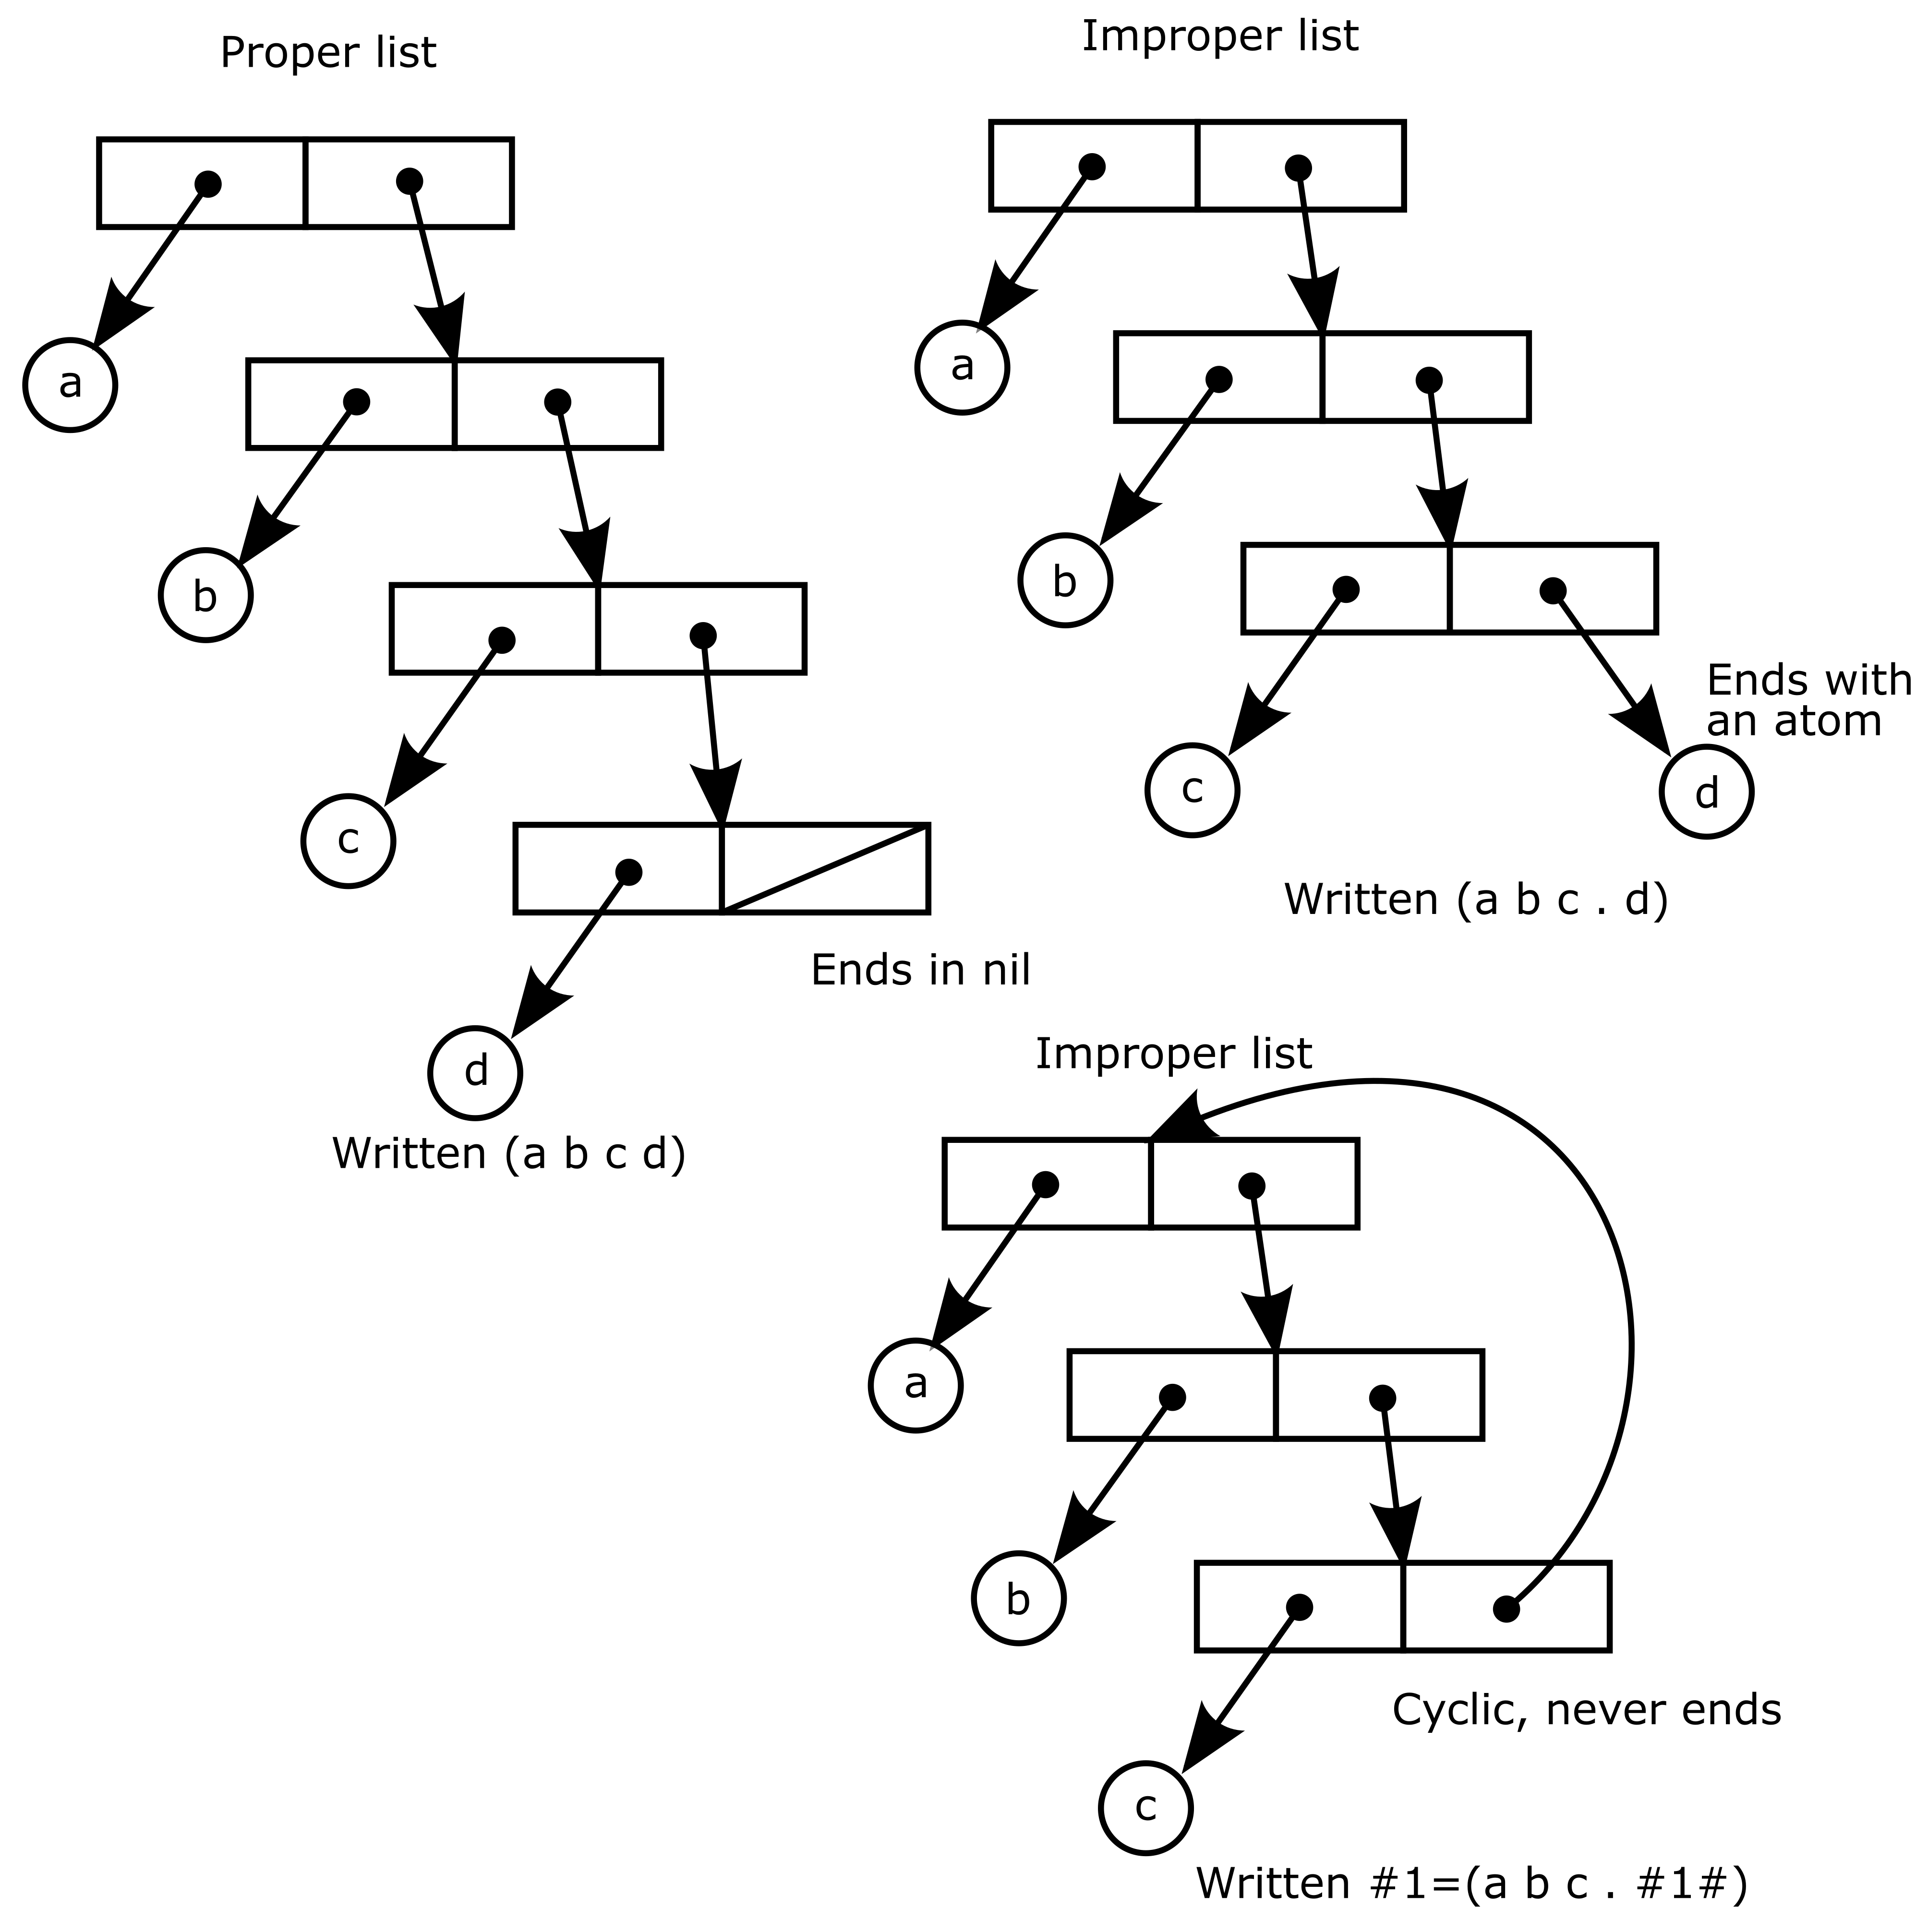
\includegraphics{images/prop-improp.png}\captionsetup{labelformat=empty}\caption{ A proper list and two improper ones.}\label{fig:-a-proper-list-and-two-improper-ones}\end{figure}
\section{Unfinished code in file input.ans line 756}
\noindent\begin{tabular}{ |p{1.9cm} p{8cm}| }
\hline
\rowcolor[HTML]{CCCCCC} \multicolumn{2}{|l|}{\bf read-pair-expr (internal)} \\
char & the terminating paren or bracket \\
\textit{Returns:} & a structure of pair expressions or end of file \\
\hline
\end{tabular}
\section{Unfinished code in file input.ans line 760}
\begin{lstlisting}
proc ::constcl::read-pair-expr {char} {
  upvar c c unget unget
  set unget {}
  set expr [read-pair $char]
  read-eof $expr
  if {$c ne $char} {
    if {$char eq ")"} {
      ::error \
        "Missing right paren. ($c)."
    } else {
      ::error \
        "Missing right bracket ($c)."
    }
  } else {
    set unget {}
    set c [readc]
  }
  return $expr
}
\end{lstlisting}
\section{Unfinished code in file input.ans line 782}

\section{Unfinished code in file input.ans line 785}

\textbf{read-pair} procedure \texttt{read-pair} is a helper procedure that does the heavy lifting in reading a pair structure. First it checks if the list is empty, returning \texttt{\#NIL} in that case. Otherwise it reads the first element in the list and then repeatedly the rest of them. If it reads a Dot object, the following element to be read is the tail end of an improper list. When \texttt{read-pair} has reached the ending parenthesis or bracket, it conses up the elements starting from the last, and returns the head of the list. Shares the variables \texttt{c} and \texttt{unget} with its caller.

\section{Unfinished code in file input.ans line 795}
\index{read-pair}
\begin{lstlisting}
proc ::constcl::read-pair {char} {
  upvar c c unget unget
  set c [readc]
  read-eof $c
  if {[T [find-char? $char]]} {
    # read right paren/brack
    #set c [readc]
    return #NIL
  }
  set a [read-expr $c]
  set res $a
  skip-ws
  set prev #NIL
  while {[find-char? $char] eq "#f"} {
    set x [read-expr $c]
    skip-ws
    read-eof $c
    if {[T [dot? $x]]} {
      set prev [read-expr $c]
      skip-ws
      read-eof $c
    } else {
      lappend res $x
    }
    if {[llength $res] > 99} break
  }
  # read right paren/brack
  foreach r [lreverse $res] {
    set prev [cons $r $prev]
  }
  return $prev
}
\end{lstlisting}
\section{Unfinished code in file input.ans line 831}
\section{Unfinished code in file input.ans line 836}
\section{Unfinished code in file input.ans line 840}
\section{Unfinished code in file input.ans line 845}
\section{Unfinished code in file input.ans line 849}
\section{Unfinished code in file input.ans line 853}
\section{Unfinished code in file input.ans line 857}
\section{Unfinished code in file input.ans line 861}
\section{Unfinished code in file input.ans line 871}
\section{Unfinished code in file input.ans line 881}
\section{Unfinished code in file input.ans line 891}
\section{Unfinished code in file input.ans line 893}
\subsection{read-plus-minus procedure}
\label{read-plus-minus-procedure}
\index{read-plus-minus procedure}
\section{Unfinished code in file input.ans line 895}


\texttt{read-plus-minus} is called when a plus or minus is found in the input stream. If the next character is a digit, it delegates to the number reader. Otherwise, it returns a \texttt{+} or \texttt{-} symbol. Shares the variables \texttt{c} and \texttt{unget} with its caller.

\section{Unfinished code in file input.ans line 902}
\noindent\begin{tabular}{ |p{1.9cm} p{8cm}| }
\hline
\rowcolor[HTML]{CCCCCC} \multicolumn{2}{|l|}{\bf read-plus-minus (internal)} \\
\textit{Returns:} & either the symbols + or - or a number or end of file \\
\hline
\end{tabular}
\section{Unfinished code in file input.ans line 906}
\begin{lstlisting}
proc ::constcl::read-plus-minus {char} {
  upvar c c unget unget
  set unget {}
  set c [readc]
  read-eof $c
  if {[::string is digit -strict $c]} {
    set n [read-number-expr $c]
    read-eof $n
    if {$char eq "-"} {
      set n [- $n]
    }
    return $n
  } elseif {[::string is space -strict $c] ||
      $c in {) ]}} {
    if {$char eq "+"} {
      return [S "+"]
    } else {
      return [S "-"]
    }
  } else {
    set n [read-identifier-expr $char $c]
    read-eof $n
    return $n
  }
}
\end{lstlisting}
\section{Unfinished code in file input.ans line 934}
\section{Unfinished code in file input.ans line 940}
\section{Unfinished code in file input.ans line 946}
\section{Unfinished code in file input.ans line 958}
\subsection{read-pound procedure}
\label{read-pound-procedure}
\index{read-pound procedure}
\section{Unfinished code in file input.ans line 960}


\texttt{read-pound} is activated by \texttt{read-expr} when it reads a pound sign (\texttt{\#}). It in turn either delegates to the vector reader or the character reader, or returns boolean literals. Shares the variables \texttt{c} and \texttt{unget} with its caller.

\section{Unfinished code in file input.ans line 967}
\noindent\begin{tabular}{ |p{1.9cm} p{8cm}| }
\hline
\rowcolor[HTML]{CCCCCC} \multicolumn{2}{|l|}{\bf read-pound (internal)} \\
\textit{Returns:} & a vector, boolean, or character value or end of file \\
\hline
\end{tabular}
\section{Unfinished code in file input.ans line 971}
\begin{lstlisting}
proc ::constcl::read-pound {} {
  upvar c c unget unget
  set unget {}
  set c [readc]
  read-eof $c
  switch $c {
    (    { set n [read-vector-expr] }
    t    { if {[T [read-end?]]} {set n #t} }
    f    { if {[T [read-end?]]} {set n #f} }
    "\\" { set n [read-character-expr] }
    default {
      ::error "Illegal #-literal: #$c"
    }
  }
  return $n
}
\end{lstlisting}
\section{Unfinished code in file input.ans line 990}
\section{Unfinished code in file input.ans line 992}
\section{Unfinished code in file input.ans line 1003}
\section{Unfinished code in file input.ans line 1005}
\subsection{read-quasiquoted-expr procedure}
\label{read-quasiquoted-expr-procedure}
\index{read-quasiquoted-expr procedure}
\section{Unfinished code in file input.ans line 1007}


\texttt{read-quasiquoted-expr} is activated when there is a backquote (\texttt{`}) in the input stream. It reads an entire expression and returns it wrapped in \texttt{quasiquote}. Shares the variables \texttt{c} and \texttt{unget} with its caller.

\section{Unfinished code in file input.ans line 1014}
\noindent\begin{tabular}{ |p{1.9cm} p{8cm}| }
\hline
\rowcolor[HTML]{CCCCCC} \multicolumn{2}{|l|}{\bf read-quasiquoted-expr (internal)} \\
\textit{Returns:} & an expr. wr. in the quasiquote symbol or end of file \\
\hline
\end{tabular}
\section{Unfinished code in file input.ans line 1018}
\begin{lstlisting}
proc ::constcl::read-quasiquoted-expr {} {
  upvar c c unget unget
  set unget {}
  set expr [read-expr]
  skip-ws
  read-eof $expr
  make-constant $expr
  return [list [S quasiquote] $expr]
}
\end{lstlisting}
\section{Unfinished code in file input.ans line 1030}
\section{Unfinished code in file input.ans line 1032}
\section{Unfinished code in file input.ans line 1036}
\section{Unfinished code in file input.ans line 1046}
\section{Unfinished code in file input.ans line 1048}
\subsection{read-quoted-expr procedure}
\label{read-quoted-expr-procedure}
\index{read-quoted-expr procedure}
\section{Unfinished code in file input.ans line 1050}


\texttt{read-quoted-expr} is activated by \texttt{read-expr} when reading a single quote ('). It then reads an entire expression beyond that, returning it wrapped in a list with \texttt{quote}. The quoted expression is made constant. Shares the variables \texttt{c} and \texttt{unget} with its caller.

\section{Unfinished code in file input.ans line 1057}
\noindent\begin{tabular}{ |p{1.9cm} p{8cm}| }
\hline
\rowcolor[HTML]{CCCCCC} \multicolumn{2}{|l|}{\bf read-quoted-expr (internal)} \\
\textit{Returns:} & an expression wrapped in the quote symbol or end of file \\
\hline
\end{tabular}
\section{Unfinished code in file input.ans line 1061}
\begin{lstlisting}
proc ::constcl::read-quoted-expr {} {
  upvar c c unget unget
  set unget {}
  set expr [read-expr]
  read-eof $expr
  make-constant $expr
  return [list [S quote] $expr]
}
\end{lstlisting}
\section{Unfinished code in file input.ans line 1072}
\section{Unfinished code in file input.ans line 1074}
\section{Unfinished code in file input.ans line 1078}
\section{Unfinished code in file input.ans line 1083}
\section{Unfinished code in file input.ans line 1093}
\section{Unfinished code in file input.ans line 1095}
\subsection{read-string-expr procedure}
\label{read-string-expr-procedure}
\index{read-string-expr procedure}
\section{Unfinished code in file input.ans line 1097}


\texttt{read-string-expr} is activated by \texttt{read-expr} when it reads a double quote. It collects characters until it reaches another (unescaped) double quote. To have double quotes in the string, escape them with backslash (which also means that backslashes have to be escaped with backslash). A backslash+n pair of characters denotes a newline (this is a ConsTcl extension). It then returns a string expression--an immutable String (see page \pageref{strings}) object. Shares the variables \texttt{c} and \texttt{unget} with its caller.

\section{Unfinished code in file input.ans line 1107}
\noindent\begin{tabular}{ |p{1.9cm} p{8cm}| }
\hline
\rowcolor[HTML]{CCCCCC} \multicolumn{2}{|l|}{\bf read-string-expr (internal)} \\
\textit{Returns:} & a string or end of file \\
\hline
\end{tabular}
\section{Unfinished code in file input.ans line 1111}
\begin{lstlisting}
proc ::constcl::read-string-expr {} {
  upvar c c unget unget
  set str {}
  set c [readc]
  read-eof $c
  while {$c ne "\"" && $c ne "#EOF"} {
    if {$c eq "\\"} {
      ::append str $c
      set c [readc]
    }
    ::append str $c
    set c [readc]
  }
  if {$c eq "#EOF"} {
    error "bad string (no ending double quote)"
  }
  set c [readc]
  set expr [MkString $str]
  read-eof $expr
  $expr mkconstant
  return $expr
}
\end{lstlisting}
\section{Unfinished code in file input.ans line 1136}
\section{Unfinished code in file input.ans line 1138}
\section{Unfinished code in file input.ans line 1143}
\section{Unfinished code in file input.ans line 1148}
\section{Unfinished code in file input.ans line 1153}
\section{Unfinished code in file input.ans line 1163}
\section{Unfinished code in file input.ans line 1173}
\section{Unfinished code in file input.ans line 1175}
\subsection{read-unquoted-expr procedure}
\label{read-unquoted-expr-procedure}
\index{read-unquoted-expr procedure}
\section{Unfinished code in file input.ans line 1177}


When a comma is found in the input stream, \texttt{read-unquoted-expr} is activated. If it reads an at-sign (\texttt{@}) it selects the symbol \texttt{unquote-splicing}, otherwise it selects the symbol \texttt{unquote}. Then it reads an entire expression and returns it wrapped in the selected symbol. Both of these expressions are only supposed to occur inside a quasiquoted expression. Shares the variables \texttt{c} and \texttt{unget} with its caller.

\section{Unfinished code in file input.ans line 1186}
\noindent\begin{tabular}{ |p{1.9cm} p{8cm}| }
\hline
\rowcolor[HTML]{CCCCCC} \multicolumn{2}{|l|}{\bf read-unquoted-expr (internal)} \\
\textit{Returns:} & an expr. wr. in the unquote/-splicing symbol or end of file \\
\hline
\end{tabular}
\section{Unfinished code in file input.ans line 1190}
\begin{lstlisting}
proc ::constcl::read-unquoted-expr {} {
  upvar c c unget unget
  set unget {}
  set c [readc]
  read-eof $c
  if {$c eq "@"} {
    set symbol "unquote-splicing"
    set expr [read-expr]
  } else {
    set symbol "unquote"
    set expr [read-expr $c]
  }
  read-eof $expr
  return [list [S $symbol] $expr]
}
\end{lstlisting}
\section{Unfinished code in file input.ans line 1208}
\section{Unfinished code in file input.ans line 1210}
\section{Unfinished code in file input.ans line 1214}
\section{Unfinished code in file input.ans line 1225}
\section{Unfinished code in file input.ans line 1227}
\subsection{read-vector-expr procedure}
\label{read-vector-expr-procedure}
\index{read-vector-expr procedure}
\section{Unfinished code in file input.ans line 1229}


\texttt{read-vector-expr} is activated by \texttt{read-pound} and reads a number of expressions until it finds an ending parenthesis. It produces a vector expression and returns a Vector (see page \pageref{vectors}) object. Shares the variables \texttt{c} and \texttt{unget} with its caller.

\section{Unfinished code in file input.ans line 1236}
\noindent\begin{tabular}{ |p{1.9cm} p{8cm}| }
\hline
\rowcolor[HTML]{CCCCCC} \multicolumn{2}{|l|}{\bf read-vector-expr (internal)} \\
\textit{Returns:} & a vector or end of file \\
\hline
\end{tabular}
\section{Unfinished code in file input.ans line 1240}
\begin{lstlisting}
proc ::constcl::read-vector-expr {} {
  upvar c c unget unget
  set res {}
  set last {}
  set c [readc]
  while {$c ne "#EOF" && $c ne ")"} {
    set e [cons [read-expr $c] #NIL]
    if {$res eq {}} {
      set res $e
      set last $e
    } else {
      set-cdr! $last $e
      set last $e
    }
    skip-ws
    read-eof $c
  }
  if {$c ne ")"} {
    ::error "Missing right paren. ($c)."
  }
  set unget {}
  set c [readc]
  set expr [MkVector $res]
  read-eof $expr
  $expr mkconstant
  return $expr
}
\end{lstlisting}
\section{Unfinished code in file input.ans line 1270}
\section{Unfinished code in file input.ans line 1272}
\section{Unfinished code in file input.ans line 1276}
\section{Unfinished code in file input.ans line 1280}
\section{Unfinished code in file input.ans line 1291}
\section{Unfinished code in file input.ans line 1293}
\section{Unfinished code in file eval.ans line 3}
\chapter{Evaluation}
\label{evaluation}
\section{Unfinished code in file eval.ans line 5}


The second thing an interpreter must be able to do is to reduce expressions to their \emph{normal form}, or \emph{evaluate}\index{eval}\index{evaluator} them. As an example, 2 + 6 and 8 are two expressions that have the same value, but the latter is in normal form (can't be reduced further) and the former is not.

\section{Unfinished code in file eval.ans line 12}
\section{The evaluator}
\label{the-evaluator}
\index{The evaluator}
\section{Unfinished code in file eval.ans line 14}

\section{Unfinished code in file eval.ans line 17}
\section{Unfinished code in file eval.ans line 20}

\textbf{eval} procedure The heart of the Lisp interpreter, \texttt{eval} takes a Lisp expression and processes it according to its syntactic form. \texttt{eval} also does two kinds of rewriting of expressions: 1) \emph{macro expansion} on a non-atomic expression into a more concrete expression. See the part about macros (see page \pageref{macros}) below, and 2) resolving \emph{local defines}, acting on expressions of the form \texttt{(begin (define \ldots } when in a local environment. See the part about resolving local defines (see page \pageref{resolving-local-defines}).

\section{Unfinished code in file eval.ans line 27}
\noindent\begin{tabular}{ |p{1.9cm} p{8cm}| }
\hline
\rowcolor[HTML]{CCCCCC} \multicolumn{2}{|l|}{\bf eval (public)} \\
expr & an expression \\
env & an environment \\
\textit{Returns:} & a Lisp value \\
\hline
\end{tabular}
\section{Unfinished code in file eval.ans line 31}
\index{eval}
\begin{lstlisting}
reg eval
\section{Unfinished code in file eval.ans line 35}
proc ::constcl::eval \
  {expr {env ::constcl::global_env}} {
  if {[T [symbol? $expr]]} {
    lookup $expr $env
  } elseif {[T [null? $expr]] ||
    [T [atom? $expr]]} {
    set expr
  } else {
    while {[[car $expr] name] in
      $::constcl::macrolist} {
      set expr [expand-macro $expr $env]
    }
    set op [car $expr]
    set args [cdr $expr]
    if {$env ne "::constcl::global_env" &&
      [$op name] eq "begin" &&
      ([T [pair? [car $args]]] &&
      [[caar $args] name] eq "define")} {
      set expr [resolve-local-defines $args]
      set op [car $expr]
      set args [cdr $expr]
    }
    switch [$op name] {
      quote {
        usage [parse "(quote datum)"] $expr
        car $args
      }
      if {
        if {[T [null? [cddr $args]]]} {
          usage [p "(if cond cons)"] $expr
          /if1 {[eval [car $args] $env]} \
            {eval [cadr $args] $env}
        } {
          usage [p "(if cond cons altr)"] $expr
          /if {[eval [car $args] $env]} \
            {eval [cadr $args] $env} \
            {eval [caddr $args] $env}
        }
      }
      begin {
        /begin $args $env
      }
      define {
        usage [p "(define sym val)"] $expr
        /define [car $args] [
          eval [cadr $args] $env] $env
      }
      set! {
        usage [p "(set! sym val)"] $expr
        /set! [car $args] [
          eval [cadr $args] $env] $env 
      }
      lambda {
        # no point checking usage here
        /lambda [car $args] [
          cdr $args] $env
      }
      default {
        invoke [eval $op $env] [
          eval-list $args $env]
      }
    }
  }
}
\end{lstlisting}
\section{Unfinished code in file eval.ans line 101}
\section{Syntactic forms}
\label{syntactic-forms}
\index{Syntactic forms}
\section{Unfinished code in file eval.ans line 103}


There are nine diffent forms or classes of expressions in Lisp:

\section{Unfinished code in file eval.ans line 107}
\begin{enumerate}
\item  variable reference
\item  constant literal
\item  quotation
\item  conditional
\item  sequence
\item  definition
\item  assignment
\item  procedure definition
\item  procedure call
\section{Unfinished code in file eval.ans line 117}
\end{enumerate}
\section{Unfinished code in file eval.ans line 124}
\subsection{Variable reference}
\label{variable-reference}
\index{Variable reference}
\section{Unfinished code in file eval.ans line 126}


\emph{Example: \texttt{r} $\Rightarrow$ 10 (a symbol \texttt{r} is evaluated to 10)}

\section{Unfinished code in file eval.ans line 129}
\section{Unfinished code in file eval.ans line 136}

A variable\index{variable}\index{variable reference} is an identifier (symbol) bound to a location in the environment. If an expression consists of an identifier it is evaluated to the value stored in that location. This is handled by the helper procedure \texttt{lookup}. It searches the environment chain for the identifier, and returns the value stored in the location it is bound to. It is an error to do lookup on an unbound symbol. \textbf{lookup} procedure

\section{Unfinished code in file eval.ans line 139}
\noindent\begin{tabular}{ |p{1.9cm} p{8cm}| }
\hline
\rowcolor[HTML]{CCCCCC} \multicolumn{2}{|l|}{\bf lookup (internal)} \\
sym & a symbol \\
env & an environment \\
\textit{Returns:} & a Lisp value \\
\hline
\end{tabular}
\section{Unfinished code in file eval.ans line 143}
\index{lookup}
\begin{lstlisting}
proc ::constcl::lookup {sym env} {
  [$env find $sym] get $sym
}
\end{lstlisting}
\section{Unfinished code in file eval.ans line 150}
\section{Unfinished code in file eval.ans line 155}
\section{Unfinished code in file eval.ans line 160}
\subsection{Constant literal}
\label{constant-literal}
\index{Constant literal}
\section{Unfinished code in file eval.ans line 162}


\emph{Example: \texttt{99} $\Rightarrow$ 99 (a number evaluates to itself)}

\section{Unfinished code in file eval.ans line 165}

Not just numbers\index{constant literal} but booleans, characters, strings, and vectors evaluate to themselves, to their innate value. Because of this, they are called autoquoting types (see next paragraph).

\section{Unfinished code in file eval.ans line 170}
\section{Unfinished code in file eval.ans line 176}
\subsection{Quotation}
\label{quotation}
\index{Quotation}
\section{Unfinished code in file eval.ans line 178}


\emph{Example: \texttt{(quote r)} $\Rightarrow$ \texttt{r} (quotation makes the symbol evaluate to itself, like a constant)}

\section{Unfinished code in file eval.ans line 181}

According to the rules of variable reference, a symbol evaluates to its stored value. Well, sometimes one wishes to use the symbol itself as a value. That is what quotation\index{quotation} is for. \texttt{(quote x)} evaluates to the symbol \texttt{x} itself and not to any value that might be stored under it. This is so common that there is a shorthand notation for it: \texttt{'x} is interpreted as \texttt{(quote x)} by the Lisp reader.

\section{Unfinished code in file eval.ans line 189}
\section{Unfinished code in file eval.ans line 194}
\section{Unfinished code in file eval.ans line 198}
\section{Unfinished code in file eval.ans line 203}
\subsection{Conditional}
\label{conditional}
\index{Conditional}
\section{Unfinished code in file eval.ans line 205}


\emph{Example: \texttt{(if (> 99 100) (* 2 2) (+ 2 4))} $\Rightarrow$ 6}

\section{Unfinished code in file eval.ans line 208}
\section{Unfinished code in file eval.ans line 215}
\section{Unfinished code in file eval.ans line 219}

The conditional\index{conditional} form \texttt{if} evaluates a Lisp list of three expressions. The first, the \emph{condition}, is evaluated first. If it evaluates to anything other than \texttt{\#f} (false), the second expression (the \emph{consequent}) is evaluated and the value returned. Otherwise, the third expression (the \emph{alternate}) is evaluated and the value returned. One of the two latter expressions will be evaluated, and the other will remain unevaluated. The two procedures that handle the conditional form are \texttt{/if} and \texttt{/if1}. The former takes both a consequent and an alternate, the latter takes only a consequent. \textbf{/if} procedure \textbf{/if1} procedure

\section{Unfinished code in file eval.ans line 223}
\noindent\begin{tabular}{ |p{1.9cm} p{8cm}| }
\hline
\rowcolor[HTML]{CCCCCC} \multicolumn{2}{|l|}{\bf /if (internal)} \\
condition & an expression \\
consequent & an expression \\
alternate & an expression \\
\textit{Returns:} & a Lisp value \\
\hline
\end{tabular}
\section{Unfinished code in file eval.ans line 227}
\noindent\begin{tabular}{ |p{1.9cm} p{8cm}| }
\hline
\rowcolor[HTML]{CCCCCC} \multicolumn{2}{|l|}{\bf /if1 (internal)} \\
condition & an expression \\
consequent & an expression \\
\textit{Returns:} & a Lisp value \\
\hline
\end{tabular}
\section{Unfinished code in file eval.ans line 231}
\index{/if}
\index{/if1}
\begin{lstlisting}
proc ::constcl::/if {cond conseq altern} {
  if {[T [uplevel [::list expr $cond]]]} {
    uplevel $conseq
  } {
    uplevel $altern
  }
}
\section{Unfinished code in file eval.ans line 242}
proc ::constcl::/if1 {cond conseq} {
  if {[T [uplevel [::list expr $cond]]]} {
    uplevel $conseq
  }
}
\end{lstlisting}
\section{Unfinished code in file eval.ans line 249}
\section{Unfinished code in file eval.ans line 254}
\section{Unfinished code in file eval.ans line 259}
\subsection{Sequence}
\label{sequence}
\index{Sequence}
\section{Unfinished code in file eval.ans line 261}


\emph{Example: \texttt{(begin (define r 10) (* r r))} $\Rightarrow$ 100}

\section{Unfinished code in file eval.ans line 264}
\section{Unfinished code in file eval.ans line 271}

When expressions are evaluated in sequence\index{sequence}, the order is important for two reasons. If the expressions have any side effects, they happen in the same order of sequence. Also, if expressions are part of a pipeline of calculations, then they need to be processed in the order of that pipeline. The \texttt{/begin} helper procedure takes a Lisp list of expressions and evaluates them in sequence, returning the value of the last one. \textbf{/begin} procedure

\section{Unfinished code in file eval.ans line 274}
\noindent\begin{tabular}{ |p{1.9cm} p{8cm}| }
\hline
\rowcolor[HTML]{CCCCCC} \multicolumn{2}{|l|}{\bf /begin (internal)} \\
exps & a Lisp list of expressions \\
env & an environment \\
\textit{Returns:} & a Lisp value \\
\hline
\end{tabular}
\section{Unfinished code in file eval.ans line 278}
\index{/begin}
\begin{lstlisting}
proc ::constcl::/begin {exps env} {
  /if {[pair? $exps]} {
    /if {[pair? [cdr $exps]]} {
      eval [car $exps] $env
      return [/begin [cdr $exps] $env]
    } {
      return [eval [car $exps] $env]
    }
  } {
    return #NIL
  }
}
\end{lstlisting}
\section{Unfinished code in file eval.ans line 294}
\section{Unfinished code in file eval.ans line 300}
\subsection{Definition}
\label{definition}
\index{Definition}
\section{Unfinished code in file eval.ans line 302}


\emph{Example: \texttt{(define r 10)} $\Rightarrow$ \ldots  (a definition doesn't evaluate to anything)}

\section{Unfinished code in file eval.ans line 305}
\section{Unfinished code in file eval.ans line 312}

We've already seen the relationship between symbols and values. Through (variable) definition\index{variable definition}\index{definition}, a symbol is bound to a value (or rather to the location the value is in), creating a variable. The \texttt{/define} helper procedure adds a variable to the current environment. It first checks that the symbol name is a valid identifier, then it updates the environment with the new binding. \textbf{/define} procedure

\section{Unfinished code in file eval.ans line 315}
\noindent\begin{tabular}{ |p{1.9cm} p{8cm}| }
\hline
\rowcolor[HTML]{CCCCCC} \multicolumn{2}{|l|}{\bf /define (internal)} \\
sym & a symbol \\
val & a Lisp value \\
env & an environment \\
\textit{Returns:} & nothing \\
\hline
\end{tabular}
\section{Unfinished code in file eval.ans line 319}
\index{/define}
\begin{lstlisting}
proc ::constcl::/define {sym val env} {
  varcheck [idcheck [$sym name]]
  $env set $sym $val
  return
}
\end{lstlisting}
\section{Unfinished code in file eval.ans line 328}
\section{Unfinished code in file eval.ans line 334}
\section{Unfinished code in file eval.ans line 338}
\section{Unfinished code in file eval.ans line 343}
\subsection{Assignment}
\label{assignment}
\index{Assignment}
\section{Unfinished code in file eval.ans line 345}


\emph{Example: \texttt{(set! r 20)} $\Rightarrow$ 20 (\texttt{r} is a bound symbol, so it's allowed to assign to it)}

\section{Unfinished code in file eval.ans line 348}
\section{Unfinished code in file eval.ans line 357}

Once a variable has been created, the value at the location it is bound to can be changed (hence the name `variable', something that can vary). The process is called assignment\index{assignment}. The \texttt{/set!} helper does assignment: it modifies an existing variable that is bound somewhere in the environment chain. It finds the variable's environment and updates the binding. It returns the value, so calls to \texttt{set!} can be chained: \texttt{(set! foo (set! bar 99))} sets both variables to 99. By Scheme convention, procedures that modify variables have `!' at the end of their name. \textbf{/set!} procedure

\section{Unfinished code in file eval.ans line 360}
\noindent\begin{tabular}{ |p{1.9cm} p{8cm}| }
\hline
\rowcolor[HTML]{CCCCCC} \multicolumn{2}{|l|}{\bf /set! (internal)} \\
var & a bound symbol \\
val & a Lisp value \\
env & an environment \\
\textit{Returns:} & a Lisp value \\
\hline
\end{tabular}
\section{Unfinished code in file eval.ans line 364}
\index{/set"!}
\begin{lstlisting}
proc ::constcl::/set! {var val env} {
  [$env find $var] set $var $val
  set val
}
\end{lstlisting}
\section{Unfinished code in file eval.ans line 372}
\section{Unfinished code in file eval.ans line 380}
\subsection{Procedure definition}
\label{procedure-definition}
\index{Procedure definition}
\section{Unfinished code in file eval.ans line 382}


\emph{Example: \texttt{(lambda (r) (* r r))} $\Rightarrow$ \texttt{::oo::Obj3601} (it will be a different object each time)}

\section{Unfinished code in file eval.ans line 385}
\section{Unfinished code in file eval.ans line 393}
\section{Unfinished code in file eval.ans line 402}
\section{Unfinished code in file eval.ans line 406}
\section{Unfinished code in file eval.ans line 410}
\section{Unfinished code in file eval.ans line 415}
\subsubsection{Scheme formals lists: an aside}
\label{scheme-formals-lists-an-aside}
\index{Scheme formals lists: an aside}
\section{Unfinished code in file eval.ans line 417}
\section{Unfinished code in file eval.ans line 419}
\begin{itemize}
\item  An \emph{empty list}, \texttt{()}, meaning that no arguments are accepted,
\item  A \emph{proper list}, \texttt{(a b c)}, meaning it accepts three arguments, one in each symbol,
\item  A \emph{symbol}, \texttt{a}, meaning that all arguments go into \texttt{a}, or
\item  A \emph{dotted list}, \texttt{(a b . c)}, meaning that two arguments go into \texttt{a} and \texttt{b}, and the rest into \texttt{c}.
\section{Unfinished code in file eval.ans line 424}
\end{itemize}

In Lisp, procedures are values just like numbers or characters. They can be defined\index{procedure definition} as the value of a symbol, passed to other procedures, and returned from procedures. One diffence from most values is that procedures need to be defined. Two questions must answered: what is the procedure meant to do? The code that does that will form the body of the procedure. Also, what, if any, items of data will have to be provided to the procedure to make it possible to calculate its result? As an example, imagine that we want to have a procedure that calculates the square (\texttt{x * x}) of a given number. In Lisp, expressions are written with the operator first and then the operands\index{operator operand order}: \texttt{(* x x)}. That is the body of the procedure. Now, what data will we have to provide to the procedure to make it work? A value stored in the variable \texttt{x} will do. It's only a single variable, but by custom we need to put it in a list: \texttt{(x)}. The operator that defines procedures is called \texttt{lambda}\index{lambda}, and we define the function with \texttt{(lambda (x) (* x x))}. One more step is needed before we can use the procedure. It must have a name. We could define it like this: \texttt{(define square (lambda (x) (* x x)))} but there is actually a shortcut notation for it: \texttt{(define (square x) (* x x))}. Now, \texttt{square} is pretty tame. How about the \texttt{hypotenuse} procedure? \texttt{(define (hypotenuse a b) (sqrt (+ (square a) (square b))))}. It calculates the square root of the sum of two squares. Under the hood, the helper \texttt{/lambda} makes a Procedure (see page \pageref{control}) object. First it needs to convert the Lisp list \texttt{body}. It is packed inside a \texttt{begin} if it has more than one expression (\texttt{S begin} stands for `the symbol begin'.), and taken out of its list if not. The Lisp list \texttt{formals} is passed on as it is. A Scheme formals list\index{formals list} is either:

\section{Unfinished code in file eval.ans line 427}
\noindent\begin{tabular}{ |p{1.9cm} p{8cm}| }
\hline
\rowcolor[HTML]{CCCCCC} \multicolumn{2}{|l|}{\bf /lambda (internal)} \\
formals & a Scheme formals list \\
body & a Lisp list of expressions \\
env & an environment \\
\textit{Returns:} & a procedure \\
\hline
\end{tabular}
\section{Unfinished code in file eval.ans line 431}
\index{/lambda}
\begin{lstlisting}
proc ::constcl::/lambda {formals body env} {
  if {[[length $body] value] > 1} {
    set body [cons [S begin] $body]
  } else {
    set body [car $body]
  }
  return [MkProcedure $formals $body $env]
}
\end{lstlisting}
\section{Unfinished code in file eval.ans line 443}
\section{Unfinished code in file eval.ans line 450}
\subsection{Procedure call}
\label{procedure-call}
\index{Procedure call}
\section{Unfinished code in file eval.ans line 452}


\emph{Example: \texttt{(+ 1 6)} $\Rightarrow$ 7}

\section{Unfinished code in file eval.ans line 455}
\section{Unfinished code in file eval.ans line 461}
\section{Unfinished code in file eval.ans line 465}

Once we have procedures, we can call\index{procedure call} them to have their calculations performed and yield results. The procedure name is put in the operator position at the front of a list, and the operands follow in the rest of the list. Our \texttt{square} procedure would be called for instance like this: \texttt{(square 11)}, and it will return 121. \texttt{invoke} arranges for a procedure to be called with each of the values in the \emph{argument list} (the list of operands). It checks if \emph{pr} really is a procedure, and determines whether to call \emph{pr} as an object or as a Tcl command. \textbf{invoke} procedure

\section{Unfinished code in file eval.ans line 468}
\noindent\begin{tabular}{ |p{1.9cm} p{8cm}| }
\hline
\rowcolor[HTML]{CCCCCC} \multicolumn{2}{|l|}{\bf invoke (internal)} \\
pr & a procedure \\
vals & a Lisp list of Lisp values \\
\textit{Returns:} & what pr returns \\
\hline
\end{tabular}
\section{Unfinished code in file eval.ans line 472}
\index{invoke}
\begin{lstlisting}
proc ::constcl::invoke {pr vals} {
  check {procedure? $pr} {
    PROCEDURE expected\n([$pr show] val ...)
  }
  if {[info object isa object $pr]} {
    $pr call {*}[splitlist $vals]
  } else {
    $pr {*}[splitlist $vals]
  }
}
\end{lstlisting}
\section{Unfinished code in file eval.ans line 486}
\section{Unfinished code in file eval.ans line 491}
\section{Unfinished code in file eval.ans line 496}

\section{Unfinished code in file eval.ans line 499}

\textbf{splitlist} procedure \texttt{splitlist} converts a Lisp list to a Tcl list with Lisp objects.

\section{Unfinished code in file eval.ans line 502}
\noindent\begin{tabular}{ |p{1.9cm} p{8cm}| }
\hline
\rowcolor[HTML]{CCCCCC} \multicolumn{2}{|l|}{\bf splitlist (internal)} \\
vals & a Lisp list of Lisp values \\
\textit{Returns:} & a Tcl list of Lisp values \\
\hline
\end{tabular}
\section{Unfinished code in file eval.ans line 506}
\index{splitlist}
\begin{lstlisting}
proc ::constcl::splitlist {vals} {
  set result {}
  while {[T [pair? $vals]]} {
    lappend result [car $vals]
    set vals [cdr $vals]
  }
  return $result
}
\end{lstlisting}
\section{Unfinished code in file eval.ans line 518}

\section{Unfinished code in file eval.ans line 521}

\textbf{eval-list} procedure \texttt{eval-list} successively evaluates the elements of a Lisp list and returns the collected results as a Lisp list.

\section{Unfinished code in file eval.ans line 525}
\noindent\begin{tabular}{ |p{1.9cm} p{8cm}| }
\hline
\rowcolor[HTML]{CCCCCC} \multicolumn{2}{|l|}{\bf eval-list (internal)} \\
exps & a Lisp list of expressions \\
env & an environment \\
\textit{Returns:} & a Lisp list of Lisp values \\
\hline
\end{tabular}
\section{Unfinished code in file eval.ans line 529}
\index{eval-list}
\begin{lstlisting}
proc ::constcl::eval-list {exps env} {
  # don't convert to /if, it breaks (fact 100)
  if {[T [pair? $exps]]} {
    return [cons [eval [car $exps] $env] \
      [eval-list [cdr $exps] $env]]
  } {
    return #NIL
  }
}
\end{lstlisting}
\section{Unfinished code in file eval.ans line 542}
\section{Unfinished code in file eval.ans line 544}
\section{Unfinished code in file eval.ans line 551}
\section{Unfinished code in file eval.ans line 552}
\section{Unfinished code in file eval.ans line 556}
\section{Unfinished code in file eval.ans line 558}
\section{Unfinished code in file eval.ans line 564}
\section{Unfinished code in file eval.ans line 570}
\section{Unfinished code in file eval.ans line 576}
\section{Unfinished code in file macros.ans line 3}
\section{Macros}
\label{macros}
\index{Macros}
\section{Unfinished code in file macros.ans line 5}
\subsection{expand-macro procedure}
\label{expand-macro-procedure}
\index{expand-macro procedure}
\section{Unfinished code in file macros.ans line 7}

\section{Unfinished code in file macros.ans line 13}
\section{Unfinished code in file macros.ans line 21}

Macros that allow concise, abstract expressions that are automatically rewritten into other, more concrete but also more verbose expressions is one of Lisp's strong points. This interpreter does macro expansion, but the user can't define new macros--the ones available are hardcoded in the code below. \texttt{expand-macro} takes an expression and an environment as a parameter. First, the operator (\emph{op}) and operands (\emph{args}) are extracted to check if expansion is necessary (the operator \texttt{car}, for historical reasons, stands for the first element of a list, while \texttt{cdr} stands for the rest of the elements after the first in a list). If the operator is the symbol \texttt{define} and the first of the operands is something other than a Pair, then expansion is unnecessary and the procedure returns with a code to break the while loop in \texttt{eval}. The operator's symbol name is then used to select the right expansion procedure, and the whole expression and the environment is passed to it. In the end, the expanded expression is passed back to \texttt{eval}.

\section{Unfinished code in file macros.ans line 26}
\noindent\begin{tabular}{ |p{1.9cm} p{8cm}| }
\hline
\rowcolor[HTML]{CCCCCC} \multicolumn{2}{|l|}{\bf expand-macro (internal)} \\
expr & an expression \\
env & an environment \\
\textit{Returns:} & an expression \\
\hline
\end{tabular}
\section{Unfinished code in file macros.ans line 30}
\begin{lstlisting}
proc ::constcl::expand-macro {expr env} {
  set op [car $expr]
  set args [cdr $expr]
  if {[$op name] eq "define" &&
      [pair? [car $args]] eq "#f"} {
    return -code break
  }
  return [expand-[$op name] $expr $env]
}
\end{lstlisting}
\section{Unfinished code in file macros.ans line 42}
\section{Unfinished code in file macros.ans line 47}
\section{Unfinished code in file macros.ans line 49}
\subsection{expand-and procedure}
\label{expand-and-procedure}
\index{expand-and procedure}
\section{Unfinished code in file macros.ans line 51}


\texttt{expand-and} expands the \texttt{and} macro. It returns a \texttt{begin}-expression if the macro has 0 or 1 elements, and a nested \texttt{if} construct otherwise.

\section{Unfinished code in file macros.ans line 56}
\noindent\begin{tabular}{ |p{1.9cm} p{8cm}| }
\hline
\rowcolor[HTML]{CCCCCC} \multicolumn{2}{|l|}{\bf expand-and (internal)} \\
expr & an expression \\
env & an environment \\
\textit{Returns:} & an expression \\
\hline
\end{tabular}
\section{Unfinished code in file macros.ans line 60}
\begin{lstlisting}
regmacro and
\section{Unfinished code in file macros.ans line 63}
proc ::constcl::expand-and {expr env} {
  set tail [cdr $expr]
  if {[[length $tail] numval] == 0} {
    list [S begin] #t
  } elseif {[[length $tail] numval] == 1} {
    cons [S begin] $tail
  } else {
    do-and $tail #t $env
  }
}
\end{lstlisting}
\section{Unfinished code in file macros.ans line 75}

\section{Unfinished code in file macros.ans line 78}

\textbf{do-and} procedure \texttt{do-and} is called recursively for every argument of \texttt{expand-or} if there are more than one.

\section{Unfinished code in file macros.ans line 82}
\subsubsection{Quasiquote: an aside}
\label{quasiquote-an-aside}
\index{Quasiquote: an aside}
\section{Unfinished code in file macros.ans line 84}


In this and many other macro expanders I use a quasiquote\index{quasiquote} construct to lay out how the macro is to be expanded. A quasiquote starts with a backquote (\texttt{`}) instead of the single quote that precedes regular quoted material. A quasiquote allows for "unquoting" of selected parts: this is notated with a comma (\texttt{,}). \texttt{`(foo ,bar baz)} is very nearly the same as \texttt{('foo bar 'baz)}. In both cases \texttt{foo} and \texttt{baz} are constants while \texttt{bar} is a variable which will be evaluated. Like in \texttt{do-and} here, a quasiquote serves well as a templating mechanism. The variables in the quasiquote need to be a part of the environment in which the quasiquote is expanded: I use \texttt{/define} to bind them in a temporary environment.

\section{Unfinished code in file macros.ans line 97}
\noindent\begin{tabular}{ |p{1.9cm} p{8cm}| }
\hline
\rowcolor[HTML]{CCCCCC} \multicolumn{2}{|l|}{\bf do-and (internal)} \\
tail & an expression tail \\
prev & an expression \\
env & an environment \\
\textit{Returns:} & an expression \\
\hline
\end{tabular}
\section{Unfinished code in file macros.ans line 101}
\index{do-and}
\begin{lstlisting}
proc ::constcl::do-and {tail prev env} {
  if {[T [null? $tail]]} {
    return $prev
  } else {
    set env [Environment new #NIL {} $env]
    /define [S first] [car $tail] $env
    /define [S rest] [do-and [cdr $tail] \
        [car $tail] $env] $env
    set qq "`(if ,first ,rest #f)"
    set expr [expand-quasiquote [parse $qq] $env]
    $env destroy
    return $expr
  }
}
\end{lstlisting}
\section{Unfinished code in file macros.ans line 119}
\section{Unfinished code in file macros.ans line 127}
\section{Unfinished code in file macros.ans line 134}
\section{Unfinished code in file macros.ans line 136}
\subsection{expand-case procedure}
\label{expand-case-procedure}
\index{expand-case procedure}
\section{Unfinished code in file macros.ans line 138}

\section{Unfinished code in file macros.ans line 144}

The body of the \texttt{case} form consists of a key-expression and a number of clauses. Each clause has a list of values and a body. If the key-expression evaluates to a value that occurs in one of the value-lists (considered in order), that clause's body is evaluated and all other clauses are ignored. The \texttt{case} macro is expanded by \texttt{expand-case}. It expands to \texttt{'()} if there are no clauses (left), and to nested \texttt{if} constructs if there are some.

\section{Unfinished code in file macros.ans line 148}
\subsubsection{caar, cadr, cdar, and the rest: an aside}
\label{caar,-cadr,-cdar,-and-the-rest-an-aside}
\index{caar, cadr, cdar, and the rest: an aside}
\section{Unfinished code in file macros.ans line 150}


The \texttt{do-case} procedure uses extensions of the \texttt{car}/\texttt{cdr} operators like \texttt{caar} and \texttt{cdar}. \texttt{car}/\texttt{cdr} notation gets really powerful when combined to form operators from \texttt{caar} to \texttt{cddddr}. One can read \texttt{caar L} as `the first element of the first element of L', implying that the first element of \texttt{L} is a list. \texttt{cdar L} is `the rest of the elements of the first element of L', and \texttt{cadr L} is `the first element of the rest of the elements of L' or in layman's terms, the second element of L.

\section{Unfinished code in file macros.ans line 160}
\noindent\begin{tabular}{ |p{1.9cm} p{8cm}| }
\hline
\rowcolor[HTML]{CCCCCC} \multicolumn{2}{|l|}{\bf expand-case (internal)} \\
expr & an expression \\
env & an environment \\
\textit{Returns:} & an expression \\
\hline
\end{tabular}
\section{Unfinished code in file macros.ans line 164}
\begin{lstlisting}
regmacro case
\section{Unfinished code in file macros.ans line 167}
proc ::constcl::expand-case {expr env} {
  set tail [cdr $expr]
  do-case [car $tail] [cdr $tail] $env
}
\section{Unfinished code in file macros.ans line 172}
proc ::constcl::do-case {keyexpr clauses env} {
  if {[T [null? $clauses]]} {
    return [parse "'()"]
  } else {
    set keyl [caar $clauses]
    set body [cdar $clauses]
    set keyl [list [S memv] $keyexpr \
        [list [S quote] $keyl]]
    # if this is the last clause...
    if {[T [eq? [length $clauses] #1]]} {
      # ...allow 'else' in the condition
      if {[T [eq? [caar $clauses] [S else]]]} {
        set keyl #t
      }
    }
    set env [Environment new #NIL {} $env]
    /define [S keyl] $keyl $env
    /define [S body] $body $env
    /define [S rest] [
      do-case $keyexpr [cdr $clauses] $env] $env
    set qq "`(if ,keyl
               (begin ,@body)
               ,rest)"
    set expr [expand-quasiquote [parse $qq] $env]
    $env destroy
    return $expr
  }
}
\end{lstlisting}
\section{Unfinished code in file macros.ans line 202}
\section{Unfinished code in file macros.ans line 207}
\section{Unfinished code in file macros.ans line 211}
\section{Unfinished code in file macros.ans line 215}
\section{Unfinished code in file macros.ans line 220}
\subsection{expand-cond procedure}
\label{expand-cond-procedure}
\index{expand-cond procedure}
\section{Unfinished code in file macros.ans line 222}

\section{Unfinished code in file macros.ans line 227}
\section{Unfinished code in file macros.ans line 230}

The \texttt{cond} form has a list of clauses, each with a predicate and a body. The clauses is considered in order, and if a predicate evaluates to something other than \texttt{\#f} the body is evaluated and the remaining clauses are ignored. The \texttt{cond} macro is expanded by \texttt{expand-cond}. It expands to \texttt{'()} if there are no clauses (left), and to nested \texttt{if} constructs if there are some.

\section{Unfinished code in file macros.ans line 232}
\noindent\begin{tabular}{ |p{1.9cm} p{8cm}| }
\hline
\rowcolor[HTML]{CCCCCC} \multicolumn{2}{|l|}{\bf expand-cond (internal)} \\
expr & an expression \\
env & an environment \\
\textit{Returns:} & an expression \\
\hline
\end{tabular}
\section{Unfinished code in file macros.ans line 236}
\begin{lstlisting}
regmacro cond
\section{Unfinished code in file macros.ans line 239}
proc ::constcl::expand-cond {expr env} {
  return [do-cond [cdr $expr] $env]
}
\end{lstlisting}
\section{Unfinished code in file macros.ans line 244}

\section{Unfinished code in file macros.ans line 247}

\textbf{do-cond} procedure \texttt{do-cond} is called recursively for every clause of the \texttt{cond} form. It chops up the clause into predicate and body, stepping over any \texttt{=>} symbols in between. In the last clause, the predicate is allowed to be \texttt{else} (which gets translated to \texttt{\#t}). If there is no body, the body is set to the predicate. The macro is expanded to a recursive \texttt{if} form.

\section{Unfinished code in file macros.ans line 254}
\noindent\begin{tabular}{ |p{1.9cm} p{8cm}| }
\hline
\rowcolor[HTML]{CCCCCC} \multicolumn{2}{|l|}{\bf do-cond (internal)} \\
tail & a Lisp list of expressions \\
env & an environment \\
\textit{Returns:} & an expression \\
\hline
\end{tabular}
\section{Unfinished code in file macros.ans line 258}
\index{do-cond}
\begin{lstlisting}
proc ::constcl::do-cond {tail env} {
  set clauses $tail
  if {[T [null? $clauses]]} {
    return [parse "'()"]
  } else {
    set pred [caar $clauses]
    set body [cdar $clauses]
    if {[T [symbol? [car $body]]] &&
        [[car $body] name] eq "=>"} {
      set body [cddar $clauses]
    }
    # if this is the last clause...
    if {[T [eq? [length $clauses] #1]]} {
      # ...allow 'else' in the predicate
      if {[T [eq? $pred [S else]]]} {
        set pred #t
      }
    }
    if {[T [null? $body]]} {
        set body $pred
    }
    set env [Environment new #NIL {} $env]
    /define [S pred] $pred $env
    /define [S body] $body $env
    /define [S rest] [
      do-cond [cdr $clauses] $env] $env
    set qq "`(if ,pred
               (begin ,@body)
               ,rest)"
    set expr [expand-quasiquote [parse $qq] $env]
    $env destroy
    return $expr
  }
}
\end{lstlisting}
\section{Unfinished code in file macros.ans line 296}
\section{Unfinished code in file macros.ans line 301}
\section{Unfinished code in file macros.ans line 306}
\section{Unfinished code in file macros.ans line 310}
\section{Unfinished code in file macros.ans line 314}
\section{Unfinished code in file macros.ans line 318}
\section{Unfinished code in file macros.ans line 322}
\section{Unfinished code in file macros.ans line 324}
\subsection{expand-define procedure}
\label{expand-define-procedure}
\index{expand-define procedure}
\section{Unfinished code in file macros.ans line 326}

\section{Unfinished code in file macros.ans line 330}
\section{Unfinished code in file macros.ans line 332}
\section{Unfinished code in file macros.ans line 334}
\section{Unfinished code in file macros.ans line 336}

\texttt{define} has two variants, one of which requires some rewriting. It's the one with an implied \texttt{lambda} call, the one that defines a procedure. (define (\emph{symbol} \emph{formals}) \emph{body}) is transformed into (define \emph{symbol} (lambda \emph{formals} \emph{body})) which conforms better to \texttt{eval}'s standard of (define \emph{symbol} \emph{value}).

\section{Unfinished code in file macros.ans line 339}
\noindent\begin{tabular}{ |p{1.9cm} p{8cm}| }
\hline
\rowcolor[HTML]{CCCCCC} \multicolumn{2}{|l|}{\bf expand-define (internal)} \\
expr & an expression \\
env & an environment \\
\textit{Returns:} & an expression \\
\hline
\end{tabular}
\section{Unfinished code in file macros.ans line 343}
\begin{lstlisting}
regmacro define
\section{Unfinished code in file macros.ans line 346}
proc ::constcl::expand-define {expr env} {
  set tail [cdr $expr]
  set env [::constcl::Environment new #NIL {} $env]
  /define [S tail] $tail $env
  set qq "`(define ,(caar tail)
             (lambda ,(cdar tail) ,@(cdr tail)))"
  set expr [expand-quasiquote [parse $qq] $env]
  $env destroy
  return $expr
}
\end{lstlisting}
\section{Unfinished code in file macros.ans line 358}
\section{Unfinished code in file macros.ans line 363}
\section{Unfinished code in file macros.ans line 367}
\section{Unfinished code in file macros.ans line 371}
\section{Unfinished code in file macros.ans line 375}
\section{Unfinished code in file macros.ans line 377}
\subsection{expand-del! procedure}
\label{expand-del"!-procedure}
\index{expand-del"! procedure}
\section{Unfinished code in file macros.ans line 379}


The macro \texttt{del!} updates a property list. It removes a key-value pair if the key is present, or leaves the list untouched if it isn't.

\section{Unfinished code in file macros.ans line 384}
\noindent\begin{tabular}{ |p{1.9cm} p{8cm}| }
\hline
\rowcolor[HTML]{CCCCCC} \multicolumn{2}{|l|}{\bf expand-del! (internal)} \\
expr & an expression \\
env & an environment \\
\textit{Returns:} & an expression \\
\hline
\end{tabular}
\section{Unfinished code in file macros.ans line 388}
\begin{lstlisting}
regmacro del!
\section{Unfinished code in file macros.ans line 391}
proc ::constcl::expand-del! {expr env} {
  set tail [cdr $expr]
  set env [Environment new #NIL {} $env]
  if {[T [null? $tail]]} {
    ::error "too few arguments, 0 of 2"
  }
  /define [S listname] [car $tail] $env
  if {[T [null? [cdr $tail]]]} {
    ::error "too few arguments, 1 of 2"
  }
  /define [S key] [cadr $tail] $env
  set qq "`(set! ,listname
             (delete! ,listname ,key))"
  set expr [expand-quasiquote [parse $qq] $env]
  $env destroy
  return $expr
}
\end{lstlisting}
\section{Unfinished code in file macros.ans line 410}
\section{Unfinished code in file macros.ans line 416}
\section{Unfinished code in file macros.ans line 421}
\section{Unfinished code in file macros.ans line 426}
\section{Unfinished code in file macros.ans line 431}
\section{Unfinished code in file macros.ans line 436}
\section{Unfinished code in file macros.ans line 438}
\subsection{expand-for procedure}
\label{expand-for-procedure}
\index{expand-for procedure}
\section{Unfinished code in file macros.ans line 440}


The \texttt{expand-for} procedure expands the \texttt{for} macro. It returns a \texttt{begin} construct containing the iterations of each clause (multiple clauses weren't implemented for the longest time, but I brought up my strongest brain cells and they did it).

\section{Unfinished code in file macros.ans line 447}
\noindent\begin{tabular}{ |p{1.9cm} p{8cm}| }
\hline
\rowcolor[HTML]{CCCCCC} \multicolumn{2}{|l|}{\bf expand-for (internal)} \\
expr & an expression \\
env & an environment \\
\textit{Returns:} & an expression \\
\hline
\end{tabular}
\section{Unfinished code in file macros.ans line 451}
\begin{lstlisting}
regmacro for
\section{Unfinished code in file macros.ans line 454}
proc ::constcl::expand-for {expr env} {
  set tail [cdr $expr]
  set res [do-for $tail $env]
  lappend res [parse "'()"]
  return [list [S begin] {*}$res]
}
\end{lstlisting}
\section{Unfinished code in file macros.ans line 462}

\section{Unfinished code in file macros.ans line 465}

\textbf{for-seq} procedure \texttt{for-seq} is a helper procedure that sets up the sequence of values that the iteration is based on. First it evaluates the code that generates the sequence, and then it converts it to a Tcl list.

\section{Unfinished code in file macros.ans line 470}
\noindent\begin{tabular}{ |p{1.9cm} p{8cm}| }
\hline
\rowcolor[HTML]{CCCCCC} \multicolumn{2}{|l|}{\bf for-seq (internal)} \\
seq & an expression \\
env & an environment \\
\textit{Returns:} & a Tcl list of Lisp values \\
\hline
\end{tabular}
\section{Unfinished code in file macros.ans line 474}
\index{for-seq}
\begin{lstlisting}
proc ::constcl::for-seq {seq env} {
  if {[T [number? $seq]]} {
    set seq [in-range $seq]
  } else {
    set seq [eval $seq $env]
  }
  # make it a Tcl list, one way or another
  if {[T [list? $seq]]} {
    set seq [splitlist $seq]
  } elseif {[T [string? $seq]]} { 
    set seq [lmap c [split [$seq value] {}] {
      MkChar #\\$c
    }]
  } elseif {[T [vector? $seq]]} {
    set seq [$seq value]
  }
}
\end{lstlisting}
\section{Unfinished code in file macros.ans line 495}

\section{Unfinished code in file macros.ans line 498}
\section{Unfinished code in file macros.ans line 503}
\section{Unfinished code in file macros.ans line 507}

\textbf{do-for} procedure \texttt{do-for} is another helper procedure which does most of the work in the \texttt{for/*} forms. It iterates over the clauses, extracting and preparing the sequence for each, and stores each of the sequence steps in a dictionary under a double key: the identifier and the ordinal of the step. Then it creates a \texttt{let} construct for each step, in which each of the clauses' identifiers is bound to the step's value. The Tcl list of \texttt{let} constructs is returned. Each clause's sequence is supposed to be the same length as the others. One weakness of this implementation is that it doesn't ensure this, just hopes that the user does the right thing.

\section{Unfinished code in file macros.ans line 512}
\noindent\begin{tabular}{ |p{1.9cm} p{8cm}| }
\hline
\rowcolor[HTML]{CCCCCC} \multicolumn{2}{|l|}{\bf do-for (internal)} \\
tail & an expression tail \\
env & an environment \\
\textit{Returns:} & a Tcl list of expressions \\
\hline
\end{tabular}
\section{Unfinished code in file macros.ans line 516}
\index{do-for}
\begin{lstlisting}
proc ::constcl::do-for {tail env} {
  # make clauses a Tcl list
  set clauses [splitlist [car $tail]]
  set body [cdr $tail]
  set data [dict create]
  set length 0
  foreach clause $clauses {
    set id [car $clause]
    set sequence [for-seq [cadr $clause] $env]
    set length [llength $sequence]
    # save every id and step of the iteration
    for {set i 0} {$i < $length} {incr i} {
        dict set data $id $i [lindex $sequence $i]
    }
  }
  set res {}
  # for every step of the iteration...
  for {set i 0} {$i < $length} {incr i} {
    set decl {}
    # retrieve the ids
    foreach id [dict keys $data] {
      # list the id and the step
      lappend decl [
        list $id [dict get $data $id $i]]
    }
    # add to the structure of let constructs
    lappend res [list [S let] [
        list {*}$decl] {*}[splitlist $body]]
  }
  return $res
}
\end{lstlisting}
\section{Unfinished code in file macros.ans line 551}
\section{Unfinished code in file macros.ans line 556}
\section{Unfinished code in file macros.ans line 560}
\section{Unfinished code in file macros.ans line 564}
\section{Unfinished code in file macros.ans line 568}
\section{Unfinished code in file macros.ans line 570}
\subsection{expand-for/and procedure}
\label{expand-for/and-procedure}
\index{expand-for/and procedure}
\section{Unfinished code in file macros.ans line 572}

\section{Unfinished code in file macros.ans line 576}

The \texttt{expand-for/and} procedure expands the \texttt{for/and} macro. It returns an \texttt{and} construct containing the iterations of the clauses. The only differences from \texttt{expand-for} is that it doesn't add \texttt{(quote ())} and that it wraps the list of iterations in \texttt{and} instead of \texttt{begin}.

\section{Unfinished code in file macros.ans line 580}
\noindent\begin{tabular}{ |p{1.9cm} p{8cm}| }
\hline
\rowcolor[HTML]{CCCCCC} \multicolumn{2}{|l|}{\bf expand-for/and (internal)} \\
expr & an expression \\
env & an environment \\
\textit{Returns:} & an expression \\
\hline
\end{tabular}
\section{Unfinished code in file macros.ans line 584}
\begin{lstlisting}
regmacro for/and
\section{Unfinished code in file macros.ans line 587}
proc ::constcl::expand-for/and {expr env} {
  set tail [cdr $expr]
  set res [do-for $tail $env]
  return [list [S and] {*}$res]
}
\end{lstlisting}
\section{Unfinished code in file macros.ans line 594}
\section{Unfinished code in file macros.ans line 599}
\section{Unfinished code in file macros.ans line 601}
\subsection{expand-for/list procedure}
\label{expand-for/list-procedure}
\index{expand-for/list procedure}
\section{Unfinished code in file macros.ans line 603}

\section{Unfinished code in file macros.ans line 607}

The \texttt{expand-for/list} procedure expands the \texttt{for/list} macro. It returns a \texttt{list} construct containing the iterations of each clause. The only difference from \texttt{expand-for/and} is that it wraps the list of iterations in \texttt{list} instead of \texttt{and}.

\section{Unfinished code in file macros.ans line 611}
\noindent\begin{tabular}{ |p{1.9cm} p{8cm}| }
\hline
\rowcolor[HTML]{CCCCCC} \multicolumn{2}{|l|}{\bf expand for/list (internal)} \\
expr & an expression \\
env & an environment \\
\textit{Returns:} & an expression \\
\hline
\end{tabular}
\section{Unfinished code in file macros.ans line 615}
\begin{lstlisting}
regmacro for/list
\section{Unfinished code in file macros.ans line 618}
proc ::constcl::expand-for/list {expr env} {
  set tail [cdr $expr]
  set res [do-for $tail $env]
  return [list [S list] {*}$res]
}
\end{lstlisting}
\section{Unfinished code in file macros.ans line 625}
\section{Unfinished code in file macros.ans line 630}
\section{Unfinished code in file macros.ans line 634}
\section{Unfinished code in file macros.ans line 638}
\section{Unfinished code in file macros.ans line 642}
\section{Unfinished code in file macros.ans line 646}
\section{Unfinished code in file macros.ans line 650}
\section{Unfinished code in file macros.ans line 654}
\section{Unfinished code in file macros.ans line 658}
\section{Unfinished code in file macros.ans line 660}
\subsection{expand-for/or procedure}
\label{expand-for/or-procedure}
\index{expand-for/or procedure}
\section{Unfinished code in file macros.ans line 662}

\section{Unfinished code in file macros.ans line 666}

The \texttt{expand-for/or} procedure expands the \texttt{for/or} macro. It returns an \texttt{or} construct containing the iterations of each clause. The only difference from \texttt{expand-for/list} is that it wraps the list of iterations in \texttt{or} instead of \texttt{list}.

\section{Unfinished code in file macros.ans line 670}
\noindent\begin{tabular}{ |p{1.9cm} p{8cm}| }
\hline
\rowcolor[HTML]{CCCCCC} \multicolumn{2}{|l|}{\bf expand-for/or (internal)} \\
expr & an expression \\
env & an environment \\
\textit{Returns:} & an expression \\
\hline
\end{tabular}
\section{Unfinished code in file macros.ans line 674}
\begin{lstlisting}
regmacro for/or
\section{Unfinished code in file macros.ans line 677}
proc ::constcl::expand-for/or {expr env} {
  set tail [cdr $expr]
  set res [do-for $tail $env]
  return [list [S or] {*}$res]
}
\end{lstlisting}
\section{Unfinished code in file macros.ans line 684}
\section{Unfinished code in file macros.ans line 689}
\section{Unfinished code in file macros.ans line 691}
\subsection{expand-let procedure}
\label{expand-let-procedure}
\index{expand-let procedure}
\section{Unfinished code in file macros.ans line 693}

\section{Unfinished code in file macros.ans line 697}
\section{Unfinished code in file macros.ans line 707}

\texttt{expand-let} expands the named \texttt{let} and `regular' \texttt{let} macros. They ultimately expand to \texttt{lambda} constructs. Named \texttt{let} chops up the expression into \emph{variable}, \emph{bindings}, and \emph{body}. It creates a dictionary with the \emph{variable} as key and \texttt{\#f} as value. Then it fills up the dictionary with variable/value pairs from the \emph{bindings}. It uses the dictionary to build a declaration list for a \texttt{let} form, a variable list for a \texttt{lambda} form, and a procedure call. Then it assembles a \texttt{let} form with the declaration list and a body consisting of an assignment and the procedure call. The assignment binds the variable to a \texttt{lambda} form with the varlist and the original \emph{body}. The \texttt{let} form is returned, meaning that the primary expansion of the named \texttt{let} is a regular \texttt{let} form. Regular \texttt{let} chops up the original expression into \emph{bindings} and \emph{body}. It creates an empty dictionary and fills it up with variable/value pairs from the \emph{bindings}. Then it builds a \texttt{lambda} operator form with the variable list, the \emph{body}, and the value list. The \texttt{lambda} call is returned as the expansion of the regular \texttt{let} form.

\section{Unfinished code in file macros.ans line 714}
\noindent\begin{tabular}{ |p{1.9cm} p{8cm}| }
\hline
\rowcolor[HTML]{CCCCCC} \multicolumn{2}{|l|}{\bf expand-let (internal)} \\
expr & an expression \\
env & an environment \\
\textit{Returns:} & an expression \\
\hline
\end{tabular}
\section{Unfinished code in file macros.ans line 718}
\begin{lstlisting}
regmacro let
\section{Unfinished code in file macros.ans line 721}
proc ::constcl::expand-let {expr env} {
  set tail [cdr $expr]
  set env [Environment new #NIL {} $env]
  if {[T [symbol? [car $tail]]]} {
    # named let
    set variable [car $tail]
    set bindings [cadr $tail]
    set body [cddr $tail]
    set vars [dict create $variable #f]
    parse-bindings vars $bindings
    /define [S decl] [list {*}[dict values [
      dict map {k v} $vars {list $k $v}]]] $env
    /define [S variable] $variable $env
    /define [S varlist] [list {*}[lrange [
      dict keys $vars] 1 end]] $env
    /define [S body] $body $env
    /define [S call] [list {*}[
      dict keys $vars]] $env
    set qq "`(let ,decl
               (set!
                 ,variable
                 (lambda ,varlist ,@body)) ,call)"
    set expr [expand-quasiquote [parse $qq] $env]
    $env destroy
    return $expr
  } else {
    # regular let
    set bindings [car $tail]
    set body [cdr $tail]
    set vars [dict create]
    parse-bindings vars $bindings
    /define [S varlist] [list {*}[
      dict keys $vars]] $env
    /define [S body] $body $env
    /define [S vallist] [list {*}[
      dict values $vars]] $env
    set qq "`((lambda ,varlist ,@body)
               ,@vallist)"
    set expr [expand-quasiquote [parse $qq] $env]
    $env destroy
    return $expr
  }
}
\end{lstlisting}
\section{Unfinished code in file macros.ans line 766}

\section{Unfinished code in file macros.ans line 769}

\textbf{parse-bindings} procedure \texttt{parse-bindings} is a helper procedure that traverses a \texttt{let} bindings list and extracts variables and values, which it puts in a dictionary. It throws an error if a variable occurs more than once.

\section{Unfinished code in file macros.ans line 774}
\noindent\begin{tabular}{ |p{1.9cm} p{8cm}| }
\hline
\rowcolor[HTML]{CCCCCC} \multicolumn{2}{|l|}{\bf parse-bindings (internal)} \\
name & a call-by-name name \\
bindings & a Lisp list of Lisp values \\
\textit{Returns:} & nothing \\
\hline
\end{tabular}
\section{Unfinished code in file macros.ans line 778}
\index{parse-bindings}
\begin{lstlisting}
proc ::constcl::parse-bindings {name bindings} {
  upvar $name vars
  foreach binding [splitlist $bindings] {
    set var [car $binding]
    set val [cadr $binding]
    if {$var in [dict keys $vars]} {
        ::error "'$var' occurs more than once"
    }
    dict set vars $var $val
  }
  return
}
\end{lstlisting}
\section{Unfinished code in file macros.ans line 794}
\section{Unfinished code in file macros.ans line 801}
\section{Unfinished code in file macros.ans line 807}
\section{Unfinished code in file macros.ans line 816}
\section{Unfinished code in file macros.ans line 820}
\section{Unfinished code in file macros.ans line 824}
\section{Unfinished code in file macros.ans line 833}
\section{Unfinished code in file macros.ans line 835}
\subsection{expand-or procedure}
\label{expand-or-procedure}
\index{expand-or procedure}
\section{Unfinished code in file macros.ans line 837}


\texttt{expand-or} expands the \texttt{or} macro. It returns a \texttt{begin}-expression if the macro has 0 or 1 elements, and a nested \texttt{if} construct otherwise.

\section{Unfinished code in file macros.ans line 842}
\noindent\begin{tabular}{ |p{1.9cm} p{8cm}| }
\hline
\rowcolor[HTML]{CCCCCC} \multicolumn{2}{|l|}{\bf expand-or (internal)} \\
expr & an expression \\
env & an environment \\
\textit{Returns:} & an expression \\
\hline
\end{tabular}
\section{Unfinished code in file macros.ans line 846}
\begin{lstlisting}
regmacro or
\section{Unfinished code in file macros.ans line 849}
proc ::constcl::expand-or {expr env} {
  set tail [cdr $expr]
  if {[T [eq? [length $tail] #0]]} {
    return [list [S begin] #f]
  } elseif {[T [eq? [length $tail] #1]]} {
    return [cons [S begin] $tail]
  } else {
    return [do-or $tail $env]
  }
}
\end{lstlisting}
\section{Unfinished code in file macros.ans line 861}
\section{Unfinished code in file macros.ans line 869}
\section{Unfinished code in file macros.ans line 871}

\section{Unfinished code in file macros.ans line 874}

\textbf{do-or} procedure \texttt{do-or} is called recursively for each argument to \texttt{expand-or} if there are more than one argument.

\section{Unfinished code in file macros.ans line 878}
\noindent\begin{tabular}{ |p{1.9cm} p{8cm}| }
\hline
\rowcolor[HTML]{CCCCCC} \multicolumn{2}{|l|}{\bf do-or (internal)} \\
tail & an expression tail \\
env & an environment \\
\textit{Returns:} & an expression \\
\hline
\end{tabular}
\section{Unfinished code in file macros.ans line 882}
\index{do-or}
\begin{lstlisting}
proc ::constcl::do-or {tail env} {
  /if {[null? $tail]} {
    return #f
  } {
    set env [Environment new #NIL {} $env]
    /define [S first] [car $tail] $env
    /define [S rest] [do-or [cdr $tail] $env] $env
    set qq "`(let ((x ,first)) (if x x ,rest))"
    set expr [expand-quasiquote [parse $qq] $env]
    $env destroy
    return $expr
  }
}
\end{lstlisting}
\section{Unfinished code in file macros.ans line 899}
\subsection{expand-pop! procedure}
\label{expand-pop"!-procedure}
\index{expand-pop"! procedure}
\section{Unfinished code in file macros.ans line 901}


The macro \texttt{pop!} updates a list. It removes the first element.

\section{Unfinished code in file macros.ans line 905}
\noindent\begin{tabular}{ |p{1.9cm} p{8cm}| }
\hline
\rowcolor[HTML]{CCCCCC} \multicolumn{2}{|l|}{\bf expand-pop! (internal)} \\
expr & an expression \\
env & an environment \\
\textit{Returns:} & an expression \\
\hline
\end{tabular}
\section{Unfinished code in file macros.ans line 909}
\begin{lstlisting}
regmacro pop!
\section{Unfinished code in file macros.ans line 912}
proc ::constcl::expand-pop! {expr env} {
  set tail [cdr $expr]
  set env [Environment new #NIL {} $env]
  if {[T [null? $tail]]} {
      ::error "too few arguments:\n(pop! listname)"
  }
  if {[symbol? [car $tail]] eq "#f"} {
      ::error "SYMBOL expected:\n(pop! listname)"
  }
  /define [S listname] [car $tail] $env
  set qq "`(set! ,listname (cdr ,listname))"
  set expr [expand-quasiquote [parse $qq] $env]
  $env destroy
  return $expr
}
\end{lstlisting}
\section{Unfinished code in file macros.ans line 929}
\section{Unfinished code in file macros.ans line 934}
\section{Unfinished code in file macros.ans line 938}
\section{Unfinished code in file macros.ans line 942}
\section{Unfinished code in file macros.ans line 944}
\subsection{expand-push! procedure}
\label{expand-push"!-procedure}
\index{expand-push"! procedure}
\section{Unfinished code in file macros.ans line 946}


The macro \texttt{push!} updates a list. It adds a new element as the new first element.

\section{Unfinished code in file macros.ans line 950}
\noindent\begin{tabular}{ |p{1.9cm} p{8cm}| }
\hline
\rowcolor[HTML]{CCCCCC} \multicolumn{2}{|l|}{\bf expand-push! (internal)} \\
expr & an expression \\
env & an environment \\
\textit{Returns:} & an expression \\
\hline
\end{tabular}
\section{Unfinished code in file macros.ans line 954}
\begin{lstlisting}
regmacro push!
\section{Unfinished code in file macros.ans line 957}
proc ::constcl::expand-push! {expr env} {
  set tail [cdr $expr]
  set env [Environment new #NIL {} $env]
  if {[T [null? $tail]]} {
    ::error \
      "too few arguments:\n(push! obj listname)"
  }
  /define [S obj] [car $tail] $env
  if {[T [null? [cdr $tail]]]} {
    ::error \
      "too few arguments:\n(push! obj listname)"
  }
  if {[symbol? [cadr $tail]] eq "#f"} {
    ::error \
      "SYMBOL expected:\n(push! obj listname)"
  }
  /define [S listname] [cadr $tail] $env
  set qq "`(set!
             ,listname
             (cons ,obj ,listname))"
  set expr [expand-quasiquote [parse $qq] $env]
  $env destroy
  return $expr
}
\end{lstlisting}
\section{Unfinished code in file macros.ans line 983}
\section{Unfinished code in file macros.ans line 989}
\subsection{expand-put! procedure}
\label{expand-put"!-procedure}
\index{expand-put"! procedure}
\section{Unfinished code in file macros.ans line 991}


The macro \texttt{put!} updates a property list. It adds a key-value pair if the key isn't present, or changes the value in place if it is.

\section{Unfinished code in file macros.ans line 996}
\noindent\begin{tabular}{ |p{1.9cm} p{8cm}| }
\hline
\rowcolor[HTML]{CCCCCC} \multicolumn{2}{|l|}{\bf expand-put! (internal)} \\
expr & an expression \\
env & an environment \\
\textit{Returns:} & an expression \\
\hline
\end{tabular}
\section{Unfinished code in file macros.ans line 1000}
\begin{lstlisting}
regmacro put!
\section{Unfinished code in file macros.ans line 1003}
proc ::constcl::expand-put! {expr env} {
  set tail [cdr $expr]
  set env [::constcl::Environment new #NIL {} $env]
  if {[T [null? $tail]]} {
      ::error "too few arguments, 0 of 3"
  }
  /define [S name] [car $tail] $env
  if {[T [null? [cdr $tail]]]} {
      ::error "too few arguments, 1 of 3"
  }
  /define [S key] [cadr $tail] $env
  if {[T [null? [cddr $tail]]]} {
      ::error "too few arguments, 2 of 3"
  }
  /define [S val] [caddr $tail] $env
  set qq "`(let ((idx (list-find-key ,name ,key)))
             (if (< idx 0)
               (set! 
                 ,name
                 (append (list ,key ,val) ,name))
               (begin
                 (list-set! ,name (+ idx 1) ,val)
                 ,name)))"
  set expr [expand-quasiquote [parse $qq] $env]
  $env destroy
  return $expr
}
\end{lstlisting}
\section{Unfinished code in file macros.ans line 1032}
\section{Unfinished code in file macros.ans line 1037}
\section{Unfinished code in file macros.ans line 1044}
\section{Unfinished code in file macros.ans line 1051}
\section{Unfinished code in file macros.ans line 1053}
\subsection{expand-quasiquote procedure}
\label{expand-quasiquote-procedure}
\index{expand-quasiquote procedure}
\section{Unfinished code in file macros.ans line 1055}


A quasi-quote isn't a macro, but we will deal with it in this section anyway. \texttt{expand-quasiquote} traverses the quasi-quoted structure searching for \texttt{unquote} and \texttt{unquote-splicing}. This code is brittle and sprawling and I barely understand it myself.

\section{Unfinished code in file macros.ans line 1062}
\noindent\begin{tabular}{ |p{1.9cm} p{8cm}| }
\hline
\rowcolor[HTML]{CCCCCC} \multicolumn{2}{|l|}{\bf expand-quasiquote (internal)} \\
expr & an expression \\
env & an environment \\
\textit{Returns:} & an expression \\
\hline
\end{tabular}
\section{Unfinished code in file macros.ans line 1066}
\begin{lstlisting}
regmacro quasiquote
\section{Unfinished code in file macros.ans line 1069}
proc ::constcl::expand-quasiquote {expr env} {
  set tail [cdr $expr]
  set qqlevel 0
  if {[T [list? [car $tail]]]} {
    set node [car $tail]
    return [qq-visit-child $node 0 $env]
  } elseif {[T [vector? [car $tail]]]} {
    set vect [car $tail]
    set res {}
    for {set i 0} {$i < [
        [vector-length $vect] numval]} {incr i} {
      set idx [MkNumber $i]
      set vecref [vector-ref $vect $idx]
      if {[T [pair? $vecref]] &&
          [T [eq? [car $vecref] [
            S unquote]]]} {
        if {$qqlevel == 0} {
          lappend res [eval [cadr $vecref] $env]
        }
      } elseif {[T [pair? $vecref]] &&
          [T [eq? [car $vecref] [
            S unquote-splicing]]]} {
        if {$qqlevel == 0} {
          lappend res {*}[splitlist [
            eval [cadr $vecref] $env]]
        }
      } elseif {[T [atom? $vecref]]} {
        lappend res $vecref
      } else {
      }
    }
    return [list [S "vector"] {*}$res]
  }
}
\end{lstlisting}
\section{Unfinished code in file macros.ans line 1105}


\textbf{qq-visit-child} procedure

\section{Unfinished code in file macros.ans line 1109}
\noindent\begin{tabular}{ |p{1.9cm} p{8cm}| }
\hline
\rowcolor[HTML]{CCCCCC} \multicolumn{2}{|l|}{\bf qq-visit-child (internal)} \\
node & a Lisp list of expressions \\
qqlevel & a Tcl number \\
env & an environment \\
\textit{Returns:} & a Tcl list of expressions \\
\hline
\end{tabular}
\section{Unfinished code in file macros.ans line 1113}
\index{qq-visit-child}
\begin{lstlisting}
proc ::constcl::qq-visit-child {node qqlevel env} {
  if {$qqlevel < 0} {
    set qqlevel 0
  }
  if {[T [list? $node]]} {
    set res {}
    foreach child [splitlist $node] {
      if {[T [pair? $child]] &&
          [T [eq? [car $child] [S unquote]]]} {
        if {$qqlevel == 0} {
          lappend res [eval [cadr $child] $env]
        } else {
          lappend res [list [S unquote] [
            qq-visit-child [cadr $child] [
            expr {$qqlevel - 1}] $env]]
        }
      } elseif {[T [pair? $child]] &&
          [T [eq? [car $child] [
          S unquote-splicing]]]} {
        if {$qqlevel == 0} {
          lappend res {*}[splitlist [
            eval [cadr $child] $env]]
        }
      } elseif {[T [pair? $child]] &&
          [T [eq? [car $child] [S quasiquote]]]} {
        lappend res [list [S quasiquote] [car [
          qq-visit-child [cdr $child] [
            expr {$qqlevel + 1}] $env]]] 
      } elseif {[T [atom? $child]]} {
        lappend res $child
      } else {
        lappend res [
          qq-visit-child $child $qqlevel $env]
      }
    }
  }
  return [list {*}$res]
}
\end{lstlisting}
\section{Unfinished code in file macros.ans line 1155}
\section{Unfinished code in file macros.ans line 1160}
\section{Unfinished code in file macros.ans line 1169}
\section{Unfinished code in file macros.ans line 1179}
\section{Unfinished code in file macros.ans line 1181}
\section{Unfinished code in file macros.ans line 1183}
\subsection{expand-unless procedure}
\label{expand-unless-procedure}
\index{expand-unless procedure}
\section{Unfinished code in file macros.ans line 1185}


\texttt{unless} is a conditional like \texttt{if}, but it takes a number of expressions. It executes them on a false outcome of \texttt{car \$tail}.

\section{Unfinished code in file macros.ans line 1190}
\noindent\begin{tabular}{ |p{1.9cm} p{8cm}| }
\hline
\rowcolor[HTML]{CCCCCC} \multicolumn{2}{|l|}{\bf expand-unless (internal)} \\
expr & an expression \\
env & an environment \\
\textit{Returns:} & an expression \\
\hline
\end{tabular}
\section{Unfinished code in file macros.ans line 1194}
\begin{lstlisting}
regmacro unless
\section{Unfinished code in file macros.ans line 1197}
proc ::constcl::expand-unless {expr env} {
  set tail [cdr $expr]
  set env [Environment new #NIL {} $env]
  /define [S tail] $tail $env
  set qq "`(if ,(car tail)
             '()
             (begin ,@(cdr tail)))"
  set expr [expand-quasiquote [parse $qq] $env]
  $env destroy
  return $expr
}
\end{lstlisting}
\section{Unfinished code in file macros.ans line 1210}
\section{Unfinished code in file macros.ans line 1215}
\section{Unfinished code in file macros.ans line 1219}
\section{Unfinished code in file macros.ans line 1221}
\subsection{expand-when procedure}
\label{expand-when-procedure}
\index{expand-when procedure}
\section{Unfinished code in file macros.ans line 1223}


\texttt{when} is a conditional like \texttt{if}, but it takes a number of expressions. It executes them on a true outcome of \texttt{car \$tail}.

\section{Unfinished code in file macros.ans line 1228}
\noindent\begin{tabular}{ |p{1.9cm} p{8cm}| }
\hline
\rowcolor[HTML]{CCCCCC} \multicolumn{2}{|l|}{\bf expand-when (internal)} \\
expr & an expression \\
env & an environment \\
\textit{Returns:} & an expression \\
\hline
\end{tabular}
\section{Unfinished code in file macros.ans line 1232}
\begin{lstlisting}
regmacro when
\section{Unfinished code in file macros.ans line 1235}
proc ::constcl::expand-when {expr env} {
  set tail [cdr $expr]
  set env [Environment new #NIL {} $env]
  /define [S tail] $tail $env
  set qq "`(if ,(car tail)
             (begin ,@(cdr tail))
             '())"
  set expr [expand-quasiquote [parse $qq] $env]
  $env destroy
  return $expr
}
\end{lstlisting}
\section{Unfinished code in file macros.ans line 1248}
\section{Unfinished code in file macros.ans line 1250}
\section{Unfinished code in file macros.ans line 1254}
\section{Unfinished code in file macros.ans line 1258}
\section{Unfinished code in file macros.ans line 1260}
\section{Unfinished code in file rld.ans line 3}
\section{Resolving local defines}
\label{resolving-local-defines}
\index{Resolving local defines}
\section{Unfinished code in file rld.ans line 5}


This section is ported from 'Scheme 9 from Empty Space'\index{S9fES}. \texttt{resolve-local-defines} is the topmost procedure in rewriting local defines as essentially a \texttt{letrec} form. It takes a list of expressions and extracts variables and values from the defines in the beginning of the list. It builds a double lambda expression with the variables and values, and the rest of the expressions from the original list as body.

\section{Unfinished code in file rld.ans line 14}
\subsection{resolve-local-defines procedure}
\label{resolve-local-defines-procedure}
\index{resolve-local-defines procedure}
\section{Unfinished code in file rld.ans line 16}
\noindent\begin{tabular}{ |p{1.9cm} p{8cm}| }
\hline
\rowcolor[HTML]{CCCCCC} \multicolumn{2}{|l|}{\bf resolve-local-defines} \\
exps & a Lisp list of expressions \\
\textit{Returns:} & an expression \\
\hline
\end{tabular}
\section{Unfinished code in file rld.ans line 20}
\begin{lstlisting}
proc ::constcl::resolve-local-defines {exps} {
  set rest [lassign [
    extract-from-defines $exps VALS] a error]
  if {[T $error]} {
    return #NIL
  }
  set rest [lassign [
    extract-from-defines $exps VARS] v error]
  if {[T $error]} {
    return #NIL
  }
  if {$rest eq "#NIL"} {
    set rest [cons #UNS #NIL]
  }
  return [make-lambdas $v $a $rest]
}
\end{lstlisting}
\section{Unfinished code in file rld.ans line 39}
\subsection{extract-from-defines procedure}
\label{extract-from-defines-procedure}
\index{extract-from-defines procedure}
\section{Unfinished code in file rld.ans line 41}


\texttt{extract-from-defines} visits every define in the given list of expressions and extracts either a variable name or a value, depending on the state of the \emph{part} flag, from each one of them. A Tcl list of 1) the resulting list of names or values, 2) error state, and 3) the rest of the expressions in the original list is returned.

\section{Unfinished code in file rld.ans line 49}
\noindent\begin{tabular}{ |p{1.9cm} p{8cm}| }
\hline
\rowcolor[HTML]{CCCCCC} \multicolumn{2}{|l|}{\bf extract-from-defines (internal)} \\
exps & a Lisp list of expressions \\
part & a flag, VARS or VALS \\
\textit{Returns:} & a Tcl list of Lisp values \\
\hline
\end{tabular}
\section{Unfinished code in file rld.ans line 53}
\begin{lstlisting}
proc ::constcl::extract-from-defines {exps part} {
  set a #NIL
  while {$exps ne "#NIL"} {
    if {[T [atom? $exps]] ||
        [T [atom? [car $exps]]] ||
        [eq? [caar $exps] [S define]] eq "#f"} {
      break
    }
    set n [car $exps]
    set k [length $n]
    if {[list? $n] eq "#f" ||
        [$k numval] < 3 ||
        [$k numval] > 3 ||
        ([T [argument-list? [cadr $n]]] ||
        ![T [symbol? [cadr $n]]])
      eq "#f"} {
        return [::list #NIL "#t" #NIL]
      }
      if {[T [pair? [cadr $n]]]} {
        if {$part eq "VARS"} {
          set a [cons [caadr $n] $a]
        } else {
          set a [cons #NIL $a]
          set new [cons [cdadr $n] [cddr $n]]
          set new [cons [S lambda] $new]
          set-car! $a $new
        }
      } else {
        if {$part eq "VARS"} {
          set a [cons [cadr $n] $a]
        } else {
          set a [cons [caddr $n] $a]
        }
      }
      set exps [cdr $exps]
    }
    return [::list $a #f $exps]
}
\end{lstlisting}
\section{Unfinished code in file rld.ans line 94}
\subsection{argument-list? procedure}
\label{argument-list?-procedure}
\index{argument-list? procedure}
\section{Unfinished code in file rld.ans line 96}


\texttt{argument-list?} accepts a Scheme formals list and rejects other values.

\section{Unfinished code in file rld.ans line 100}
\noindent\begin{tabular}{ |p{1.9cm} p{8cm}| }
\hline
\rowcolor[HTML]{CCCCCC} \multicolumn{2}{|l|}{\bf argument-list? (internal)} \\
val & a Lisp value \\
\textit{Returns:} & a boolean \\
\hline
\end{tabular}
\section{Unfinished code in file rld.ans line 104}
\begin{lstlisting}
proc ::constcl::argument-list? {val} {
  if {$val eq "#NIL"} {
    return #t
  } elseif {[T [symbol? $val]]} {
    return #t
  } elseif {[T [atom? $val]]} {
    return #f
  }
  while {[T [pair? $val]]} {
    if {[symbol? [car $val]] eq "#f"} {
      return #f
    }
    set val [cdr $val]
  }
  if {$val eq "#NIL"} {
    return #t
  } elseif {[T [symbol? $val]]} {
    return #t
  }
}
\end{lstlisting}
\section{Unfinished code in file rld.ans line 127}
\subsection{make-lambdas procedure}
\label{make-lambdas-procedure}
\index{make-lambdas procedure}
\section{Unfinished code in file rld.ans line 129}


\texttt{make-lambdas} builds the \texttt{letrec} structure.

\section{Unfinished code in file rld.ans line 133}
\noindent\begin{tabular}{ |p{1.9cm} p{8cm}| }
\hline
\rowcolor[HTML]{CCCCCC} \multicolumn{2}{|l|}{\bf make-lambdas (internal)} \\
vars & a Lisp list of symbols \\
args & a Lisp list of expressions \\
body & a Lisp list of expressions \\
\textit{Returns:} & an expression \\
\hline
\end{tabular}
\section{Unfinished code in file rld.ans line 137}
\begin{lstlisting}
proc ::constcl::make-lambdas {vars args body} {
  set tmps [make-temporaries $vars]
  set body [append-b [
    make-assignments $vars $tmps] $body]
  set body [cons $body #NIL]
  set n [cons $tmps $body]
  set n [cons [S lambda] $n]
  set n [cons $n $args]
  set n [cons $n #NIL]
  set n [cons $vars $n]
  set n [cons [S lambda] $n]
  set n [cons $n [make-undefineds $vars]]
  return $n
}
\end{lstlisting}
\section{Unfinished code in file rld.ans line 154}
\subsection{make-temporaries procedure}
\label{make-temporaries-procedure}
\index{make-temporaries procedure}
\section{Unfinished code in file rld.ans line 156}


\texttt{make-temporaries} creates the symbols that will act as middlemen in transferring the values to the variables.

\section{Unfinished code in file rld.ans line 161}
\noindent\begin{tabular}{ |p{1.9cm} p{8cm}| }
\hline
\rowcolor[HTML]{CCCCCC} \multicolumn{2}{|l|}{\bf make-temporaries (internal)} \\
vals & a Lisp list of Lisp values \\
\textit{Returns:} & a Lisp list of Lisp values \\
\hline
\end{tabular}
\section{Unfinished code in file rld.ans line 165}
\begin{lstlisting}
proc ::constcl::make-temporaries {vals} {
  set res #NIL
  while {$vals ne "#NIL"} {
    set res [cons [gensym "g"] $res]
    set vals [cdr $vals]
  }
  return $res
}
\end{lstlisting}
\section{Unfinished code in file rld.ans line 176}
\subsection{gensym procedure}
\label{gensym-procedure}
\index{gensym procedure}
\section{Unfinished code in file rld.ans line 178}


\texttt{gensym} generates a unique symbol. The candidate symbol is compared to all the symbols in the symbol table to avoid collisions.

\section{Unfinished code in file rld.ans line 183}
\noindent\begin{tabular}{ |p{1.9cm} p{8cm}| }
\hline
\rowcolor[HTML]{CCCCCC} \multicolumn{2}{|l|}{\bf gensym (internal)} \\
prefix & a string \\
\textit{Returns:} & a symbol \\
\hline
\end{tabular}
\section{Unfinished code in file rld.ans line 187}
\begin{lstlisting}
proc ::constcl::gensym {prefix} {
  set symbolnames [
    dict keys $::constcl::symbolTable]
  set s $prefix<[incr ::constcl::gensymnum]>
  while {$s in $symbolnames} {
    set s $prefix[incr ::constcl::gensymnum]
  }
  return [S $s]
}
\end{lstlisting}
\section{Unfinished code in file rld.ans line 199}
\subsection{append-b procedure}
\label{append-b-procedure}
\index{append-b procedure}
\section{Unfinished code in file rld.ans line 201}


\texttt{append-b} joins two lists together.

\section{Unfinished code in file rld.ans line 205}
\noindent\begin{tabular}{ |p{1.9cm} p{8cm}| }
\hline
\rowcolor[HTML]{CCCCCC} \multicolumn{2}{|l|}{\bf append-b (internal)} \\
a & a Lisp list of Lisp values \\
b & a Lisp list of Lisp values \\
\textit{Returns:} & a Lisp list of Lisp values \\
\hline
\end{tabular}
\section{Unfinished code in file rld.ans line 209}
\begin{lstlisting}
proc ::constcl::append-b {a b} {
  if {$a eq "#NIL"} {
    return $b
  }
  set p $a
  while {$p ne "#NIL"} {
    if {[T [atom? $p]]} {
      ::error "append: improper list"
    }
    set last $p
    set p [cdr $p]
  }
  set-cdr! $last $b
  return $a
}
\end{lstlisting}
\section{Unfinished code in file rld.ans line 227}
\subsection{make-assignments procedure}
\label{make-assignments-procedure}
\index{make-assignments procedure}
\section{Unfinished code in file rld.ans line 229}


\texttt{make-assignments} creates the structure that holds the assignment statements. Later on, it will be joined to the body of the finished expression.

\section{Unfinished code in file rld.ans line 234}
\noindent\begin{tabular}{ |p{1.9cm} p{8cm}| }
\hline
\rowcolor[HTML]{CCCCCC} \multicolumn{2}{|l|}{\bf make-assignments (internal)} \\
vars & a Lisp list of symbols \\
tmps & a Lisp list of symbols \\
\textit{Returns:} & an expression \\
\hline
\end{tabular}
\section{Unfinished code in file rld.ans line 238}
\begin{lstlisting}
proc ::constcl::make-assignments {vars tmps} {
  set res #NIL
  while {$vars ne "#NIL"} {
    set asg [cons [car $tmps] #NIL]
    set asg [cons [car $vars] $asg]
    set asg [cons [S set!] $asg]
    set res [cons $asg $res]
    set vars [cdr $vars]
    set tmps [cdr $tmps]
  }
  return [cons [S begin] $res]
}
\end{lstlisting}
\section{Unfinished code in file rld.ans line 253}
\subsection{make-undefineds procedure}
\label{make-undefineds-procedure}
\index{make-undefineds procedure}
\section{Unfinished code in file rld.ans line 255}


Due to a mysterious bug, \texttt{make-undefineds} actually creates a list of NIL values instead of undefined values.

\section{Unfinished code in file rld.ans line 260}
\noindent\begin{tabular}{ |p{1.9cm} p{8cm}| }
\hline
\rowcolor[HTML]{CCCCCC} \multicolumn{2}{|l|}{\bf make-undefineds (internal)} \\
vals & a Lisp list of Lisp values \\
\textit{Returns:} & a Lisp list of nil values \\
\hline
\end{tabular}
\section{Unfinished code in file rld.ans line 264}
\begin{lstlisting}
proc ::constcl::make-undefineds {vals} {
  # TODO find bug, substitute #UND
  set res #NIL
  while {$vals ne "#NIL"} {
    set res [cons #NIL $res]
    set vals [cdr $vals]
  }
  return $res
}
\end{lstlisting}
\section{Unfinished code in file rld.ans line 276}
\section{Unfinished code in file rld.ans line 278}
\section{Unfinished code in file rld.ans line 283}
\section{Unfinished code in file rld.ans line 288}
\section{Unfinished code in file rld.ans line 293}
\section{Unfinished code in file rld.ans line 298}
\section{Unfinished code in file rld.ans line 303}
\section{Unfinished code in file rld.ans line 305}
\section{Unfinished code in file output.ans line 3}
\chapter{Output}
\label{output}
\section{Unfinished code in file output.ans line 5}
\subsection{write procedure}
\label{write-procedure}
\index{write procedure}
\section{Unfinished code in file output.ans line 7}

\section{Unfinished code in file output.ans line 11}

The third thing an interpreter must be able to do is to present the resulting code and data so that the user can know what the outcome of the evaluation was. As long as the object given to \texttt{write} isn't the empty string, it calls the object's \texttt{write} method and writes a newline.

\section{Unfinished code in file output.ans line 15}
\noindent\begin{tabular}{ |p{1.9cm} p{8cm}| }
\hline
\rowcolor[HTML]{CCCCCC} \multicolumn{2}{|l|}{\bf write (public)} \\
val & a Lisp value \\
?port? & a port \\
\textit{Returns:} & nothing \\
\hline
\end{tabular}
\section{Unfinished code in file output.ans line 19}
\begin{lstlisting}
reg write ::constcl::write
\section{Unfinished code in file output.ans line 22}
proc ::constcl::write {val args} {
  if {$val ne ""} {
    if {[llength $args]} {
      lassign $args port
      set dealloc 0
    } else {
      set port [MkOutputPort stdout]
      set dealloc 1
    }
    set ::constcl::Output_port $port
    $val write [$::constcl::Output_port handle]
    puts [$::constcl::Output_port handle] {}
    set ::constcl::Output_port [MkOutputPort stdout]
    if {$dealloc} {$port destroy}
  }
  return
}
\end{lstlisting}
\section{Unfinished code in file output.ans line 41}
\subsection{display procedure}
\label{display-procedure}
\index{display procedure}
\section{Unfinished code in file output.ans line 43}


The \texttt{display} procedure is like \texttt{write} but it calls the method's \texttt{display} method and doesn't print a newline.

\section{Unfinished code in file output.ans line 48}
\noindent\begin{tabular}{ |p{1.9cm} p{8cm}| }
\hline
\rowcolor[HTML]{CCCCCC} \multicolumn{2}{|l|}{\bf display (public)} \\
val & a Lisp value \\
?port? & a port \\
\textit{Returns:} & nothing \\
\hline
\end{tabular}
\section{Unfinished code in file output.ans line 52}
\begin{lstlisting}
reg display ::constcl::display
\section{Unfinished code in file output.ans line 55}
proc ::constcl::display {val args} {
  if {$val ne ""} {
    if {[llength $args]} {
      lassign $args port
      set dealloc 0
    } else {
      set port [MkOutputPort stdout]
      set dealloc 1
    }
    set ::constcl::Output_port $port
    $val display [$::constcl::Output_port handle]
    flush [$::constcl::Output_port handle]
    set ::constcl::Output_port [MkOutputPort stdout]
    if {$dealloc} {$port destroy}
  }
  return
}
\end{lstlisting}
\section{Unfinished code in file output.ans line 74}
\subsection{write-pair procedure}
\label{write-pair-procedure}
\index{write-pair procedure}
\section{Unfinished code in file output.ans line 76}


The \texttt{write-pair} procedure prints a Pair object.

\section{Unfinished code in file output.ans line 80}
\noindent\begin{tabular}{ |p{1.9cm} p{8cm}| }
\hline
\rowcolor[HTML]{CCCCCC} \multicolumn{2}{|l|}{\bf write-pair (internal)} \\
handle & a channel handle \\
pair & a pair \\
\textit{Returns:} & nothing \\
\hline
\end{tabular}
\section{Unfinished code in file output.ans line 84}
\begin{lstlisting}
proc ::constcl::write-pair {handle pair} {
  # take an object and print the car
  # and the cdr of the stored value
  set a [car $pair]
  set d [cdr $pair]
  # print car
  $a write $handle
  if {[T [pair? $d]]} {
    # cdr is a cons pair
    puts -nonewline $handle " "
    write-pair $handle $d
  } elseif {[T [null? $d]]} {
    # cdr is nil
    return
  } else {
    # it is an atom
    puts -nonewline $handle " . "
    $d write $handle
  }
  return
}
\end{lstlisting}
\section{Unfinished code in file output.ans line 108}
\section{Unfinished code in file output.ans line 110}
\section{Unfinished code in file output.ans line 114}
\section{Unfinished code in file output.ans line 118}
\section{Unfinished code in file output.ans line 122}
\section{Unfinished code in file output.ans line 124}
\chapter{Built-in procedures}
\label{built-in-procedures}
\section{Unfinished code in file equipred.ans line 4}
\section{Equivalence predicates}
\label{equivalence-predicates}
\index{Equivalence predicates}
\section{Unfinished code in file equipred.ans line 6}

\section{Unfinished code in file equipred.ans line 12}

Of the three equivalence predicates, \texttt{eq} generally tests for identity (with exception for numbers), \texttt{eqv} tests for value equality (except for booleans and procedures, where it tests for identity), and \texttt{equal} tests for whether the output strings are equal.

\subsection{eq? procedure}
\label{eq?-procedure}
\index{eq? procedure}
\section{Unfinished code in file equipred.ans line 15}
\noindent\begin{tabular}{ |p{1.9cm} p{8cm}| }
\hline
\rowcolor[HTML]{CCCCCC} \multicolumn{2}{|l|}{\bf eq?, eqv?, equal? (public)} \\
expr1 & an expression \\
expr2 & an expression \\
\textit{Returns:} & a boolean \\
\hline
\end{tabular}
\section{Unfinished code in file equipred.ans line 19}
\begin{lstlisting}
reg eq?
\section{Unfinished code in file equipred.ans line 22}
proc ::constcl::eq? {expr1 expr2} {
  if {[teq boolean? $expr1 $expr2] &&
      $expr1 eq $expr2} {
    return #t
  } elseif {[teq symbol? $expr1 $expr2] &&
      $expr1 eq $expr2} {
    return #t
  } elseif {[teq number? $expr1 $expr2] &&
      [veq $expr1 $expr2]} {
    return #t
  } elseif {[teq char? $expr1 $expr2] &&
      $expr1 eq $expr2} {
    return #t
  } elseif {[teq null? $expr1 $expr2]} {
    return #t
  } elseif {[teq pair? $expr1 $expr2] &&
      $expr1 eq $expr2} {
    return #t
  } elseif {[teq string? $expr1 $expr2] &&
      $expr1 eq $expr2} {
    return #t
  } elseif {[teq vector? $expr1 $expr2] &&
      $expr1 eq $expr2} {
    return #t
  } elseif {[teq procedure? $expr1 $expr2] &&
      $expr1 eq $expr2} {
    return #t
  } else {
    return #f
  }
}
\end{lstlisting}
\section{Unfinished code in file equipred.ans line 55}

\section{Unfinished code in file equipred.ans line 58}

\textbf{teq} procedure \texttt{teq} tests for type equality, i.e. that the expressions have the same type.

\section{Unfinished code in file equipred.ans line 61}
\noindent\begin{tabular}{ |p{1.9cm} p{8cm}| }
\hline
\rowcolor[HTML]{CCCCCC} \multicolumn{2}{|l|}{\bf teq (internal)} \\
typep & a procedure \\
expr1 & an expression \\
expr2 & an expression \\
\textit{Returns:} & a Tcl truth value (1 or 0) \\
\hline
\end{tabular}
\section{Unfinished code in file equipred.ans line 65}
\index{teq}
\begin{lstlisting}
proc ::constcl::teq {typep expr1 expr2} {
    return [expr {[T [$typep $expr1]] &&
      [T [$typep $expr2]]}]
}
\end{lstlisting}
\section{Unfinished code in file equipred.ans line 73}

\section{Unfinished code in file equipred.ans line 76}

\textbf{veq} procedure \texttt{veq} tests for value equality, i.e. that the expressions have the same value.

\section{Unfinished code in file equipred.ans line 79}
\noindent\begin{tabular}{ |p{1.9cm} p{8cm}| }
\hline
\rowcolor[HTML]{CCCCCC} \multicolumn{2}{|l|}{\bf veq (internal)} \\
expr1 & an expression \\
expr2 & an expression \\
\textit{Returns:} & a Tcl truth value (1 or 0) \\
\hline
\end{tabular}
\section{Unfinished code in file equipred.ans line 83}
\index{veq}
\begin{lstlisting}
proc ::constcl::veq {expr1 expr2} {
    return [expr {[$expr1 value] eq [$expr2 value]}]
}
\end{lstlisting}
\section{Unfinished code in file equipred.ans line 90}
\section{Unfinished code in file equipred.ans line 95}
\section{Unfinished code in file equipred.ans line 100}
\subsection{eqv? procedure}
\label{eqv?-procedure}
\index{eqv? procedure}
\section{Unfinished code in file equipred.ans line 102}
\begin{lstlisting}
reg eqv?
\section{Unfinished code in file equipred.ans line 105}
proc ::constcl::eqv? {expr1 expr2} {
  if {[teq boolean? $expr1 $expr2] &&
      $expr1 eq $expr2} {
    return #t
  } elseif {[teq symbol? $expr1 $expr2] &&
      [veq $expr1 $expr2]} {
    return #t
  } elseif {[teq number? $expr1 $expr2] &&
      [veq $expr1 $expr2]} {
    return #t
  } elseif {[teq char? $expr1 $expr2] &&
      [veq $expr1 eq $expr2]} {
    return #t
  } elseif {[teq null? $expr1 $expr2]} {
    return #t
  } elseif {[T [pair? $expr1]] &&
      [T [pair? $expr2]] &&
      [$expr1 car] eq [$expr2 car] &&
      [$expr1 cdr] eq [$expr2 cdr]} {
    return #t
  } elseif {[teq string? $expr1 $expr2] &&
      [veq $expr1 $expr2]} {
    return #t
  } elseif {[teq vector? $expr1 $expr2] &&
      [veq $expr1 $expr2]} {
    return #t
  } elseif {[teq procedure? $expr1 $expr2] &&
      $expr1 eq $expr2} {
    return #t
  } else {
    return #f
  }
}
\end{lstlisting}
\section{Unfinished code in file equipred.ans line 140}
\subsection{equal? procedure}
\label{equal?-procedure}
\index{equal? procedure}
\section{Unfinished code in file equipred.ans line 142}
\begin{lstlisting}
reg equal?
\section{Unfinished code in file equipred.ans line 145}
proc ::constcl::equal? {expr1 expr2} {
  if {[$expr1 show] eq [$expr2 show]} {
    return #t
  } else {
    return #f
  }
  # TODO
}
\end{lstlisting}
\section{Unfinished code in file equipred.ans line 155}
\section{Unfinished code in file numbers.ans line 3}
\section{Numbers}
\label{numbers}
\index{Numbers}
\section{Unfinished code in file numbers.ans line 5}

\section{Unfinished code in file numbers.ans line 11}
\subsection{Number class}
\label{number-class}
\index{Number class}
\section{Unfinished code in file numbers.ans line 13}

I have only implemented a bare-bones version of Scheme's numerical library. The following is a reasonably complete framework for operations on integers and floating-point numbers. No rationals, no complex numbers, no gcd or lcm.

\begin{lstlisting}
oo::class create ::constcl::Number {
  superclass ::constcl::NIL
  variable value
  constructor {v} {
    if {[::string is double -strict $v]} {
      set value $v
    } else {
      ::error "NUMBER expected\n$v"
    }
  }
  method zero? {} {
    if {$value == 0} {return #t} {return #f}
  }
  method positive? {} {
    if {$value > 0} {return #t} {return #f}
  }
  method negative? {} {
    if {$value < 0} {return #t} {return #f}
  }
  method even? {} {
    if {$value % 2 == 0} {return #t} {return #f}
  }
  method odd? {} {
    if {$value % 2 == 1} {return #t} {return #f}
  }
  method value {} {
    set value
  }
  method numval {} {
    set value
  }
  method mkconstant {} {}
  method constant {} {
    return 1
  }
  method write {handle} {
    puts -nonewline $handle [my value]
  }
  method display {handle} {
    my write $handle
  }
  method show {} {
    set value
  }
}
\end{lstlisting}
\section{Unfinished code in file numbers.ans line 62}
\subsection{MkNumber generator}
\label{mknumber-generator}
\index{MkNumber generator}
\section{Unfinished code in file numbers.ans line 64}


\texttt{MkNumber} generates a Number object. Short form: \texttt{N}.

\section{Unfinished code in file numbers.ans line 68}
\noindent\begin{tabular}{ |p{1.9cm} p{8cm}| }
\hline
\rowcolor[HTML]{CCCCCC} \multicolumn{2}{|l|}{\bf MkNumber (internal)} \\
str & a string \\
\textit{Returns:} & a number \\
\hline
\end{tabular}
\section{Unfinished code in file numbers.ans line 72}
\begin{lstlisting}
interp alias {} ::constcl::MkNumber \
  {} ::constcl::Number new
interp alias {} N {} ::constcl::Number new
\end{lstlisting}
\section{Unfinished code in file numbers.ans line 78}
\subsection{number? procedure}
\label{number?-procedure}
\index{number? procedure}
\section{Unfinished code in file numbers.ans line 80}


\texttt{number?} recognizes a number by object type, not by content.

\section{Unfinished code in file numbers.ans line 84}
\noindent\begin{tabular}{ |p{1.9cm} p{8cm}| }
\hline
\rowcolor[HTML]{CCCCCC} \multicolumn{2}{|l|}{\bf number? (public)} \\
val & a Lisp value \\
\textit{Returns:} & a boolean \\
\hline
\end{tabular}
\section{Unfinished code in file numbers.ans line 88}
\begin{lstlisting}
reg number?
\section{Unfinished code in file numbers.ans line 91}
proc ::constcl::number? {val} {
  return [typeof? $val Number]
}
\end{lstlisting}
\section{Unfinished code in file numbers.ans line 96}
\section{Unfinished code in file numbers.ans line 98}
\section{Unfinished code in file numbers.ans line 102}
\section{Unfinished code in file numbers.ans line 106}
\section{Unfinished code in file numbers.ans line 110}
\section{Unfinished code in file numbers.ans line 112}
\subsection{= procedure}
\label{=-procedure}
\index{= procedure}
\section{Unfinished code in file numbers.ans line 114}

\noindent \textbf{<} procedure

\section{Unfinished code in file numbers.ans line 116}

\noindent \textbf{>} procedure

\section{Unfinished code in file numbers.ans line 118}

\noindent \textbf{<=} procedure

\section{Unfinished code in file numbers.ans line 120}

\noindent \textbf{>=} procedure

\section{Unfinished code in file numbers.ans line 122}

\section{Unfinished code in file numbers.ans line 125}

The predicates \texttt{=}, \texttt{<}, \texttt{>}, \texttt{<=}, and \texttt{>=} are implemented.

\section{Unfinished code in file numbers.ans line 127}
\noindent\begin{tabular}{ |p{1.9cm} p{8cm}| }
\hline
\rowcolor[HTML]{CCCCCC} \multicolumn{2}{|l|}{\bf =, <, >, <=, >= (public)} \\
nums & some numbers \\
\textit{Returns:} & a boolean \\
\hline
\end{tabular}
\section{Unfinished code in file numbers.ans line 131}
\begin{lstlisting}
reg =
\section{Unfinished code in file numbers.ans line 134}
proc ::constcl::= {args} {
  try {
    set nums [lmap arg $args {$arg numval}]
  } on error {} {
    ::error "NUMBER expected\n(= num ...)"
  }
  if {[::tcl::mathop::== {*}$nums]} {
    return #t
  } else {
    return #f
  }
}
\end{lstlisting}
\section{Unfinished code in file numbers.ans line 148}
\section{Unfinished code in file numbers.ans line 150}
\section{Unfinished code in file numbers.ans line 154}
\section{Unfinished code in file numbers.ans line 158}
\section{Unfinished code in file numbers.ans line 160}
\index{<}
\begin{lstlisting}
reg <
\section{Unfinished code in file numbers.ans line 164}
proc ::constcl::< {args} {
  try {
    set nums [lmap arg $args {$arg numval}]
  } on error {} {
    ::error "NUMBER expected\n(< num ...)"
  }
  if {[::tcl::mathop::< {*}$nums]} {
    return #t
  } else {
    return #f
  }
}
\end{lstlisting}
\section{Unfinished code in file numbers.ans line 178}
\section{Unfinished code in file numbers.ans line 180}
\section{Unfinished code in file numbers.ans line 184}
\section{Unfinished code in file numbers.ans line 186}
\index{>}
\begin{lstlisting}
reg >
\section{Unfinished code in file numbers.ans line 190}
proc ::constcl::> {args} {
  try {
    set nums [lmap arg $args {$arg numval}]
  } on error {} {
    ::error "NUMBER expected\n(> num ...)"
  }
  if {[::tcl::mathop::> {*}$nums]} {
    return #t
  } else {
    return #f
  }
}
\end{lstlisting}
\section{Unfinished code in file numbers.ans line 204}
\section{Unfinished code in file numbers.ans line 206}
\section{Unfinished code in file numbers.ans line 210}
\section{Unfinished code in file numbers.ans line 212}
\index{<=}
\begin{lstlisting}
reg <=
\section{Unfinished code in file numbers.ans line 216}
proc ::constcl::<= {args} {
  try {
    set nums [lmap arg $args {$arg numval}]
  } on error {} {
    ::error "NUMBER expected\n(<= num ...)"
  }
  if {[::tcl::mathop::<= {*}$nums]} {
    return #t
  } else {
    return #f
  }
}
\end{lstlisting}
\section{Unfinished code in file numbers.ans line 230}
\section{Unfinished code in file numbers.ans line 232}
\section{Unfinished code in file numbers.ans line 236}
\section{Unfinished code in file numbers.ans line 238}
\index{>=}
\begin{lstlisting}
reg >=
\section{Unfinished code in file numbers.ans line 242}
proc ::constcl::>= {args} {
  try {
    set nums [lmap arg $args {$arg numval}]
  } on error {} {
    ::error "NUMBER expected\n(>= num ...)"
  }
  if {[::tcl::mathop::>= {*}$nums]} {
    return #t
  } else {
    return #f
  }
}
\end{lstlisting}
\section{Unfinished code in file numbers.ans line 256}
\section{Unfinished code in file numbers.ans line 258}
\section{Unfinished code in file numbers.ans line 262}
\section{Unfinished code in file numbers.ans line 264}
\subsection{zero? procedure}
\label{zero?-procedure}
\index{zero? procedure}
\section{Unfinished code in file numbers.ans line 266}


The \texttt{zero?} predicate tests if a given number is equal to zero.

\section{Unfinished code in file numbers.ans line 270}
\noindent\begin{tabular}{ |p{1.9cm} p{8cm}| }
\hline
\rowcolor[HTML]{CCCCCC} \multicolumn{2}{|l|}{\bf zero? (public)} \\
num & a number \\
\textit{Returns:} & a boolean \\
\hline
\end{tabular}
\section{Unfinished code in file numbers.ans line 274}
\begin{lstlisting}
reg zero?
\section{Unfinished code in file numbers.ans line 277}
proc ::constcl::zero? {num} {
  check {number? $num} {
      NUMBER expected\n([pn] [$num show])
  }
  return [$num zero?]
}
\end{lstlisting}
\section{Unfinished code in file numbers.ans line 285}
\section{Unfinished code in file numbers.ans line 287}
\section{Unfinished code in file numbers.ans line 291}
\section{Unfinished code in file numbers.ans line 295}
\section{Unfinished code in file numbers.ans line 297}
\subsection{positive? procedure}
\label{positive?-procedure}
\index{positive? procedure}
\section{Unfinished code in file numbers.ans line 299}

\noindent \textbf{negative?} procedure

\section{Unfinished code in file numbers.ans line 301}

\noindent \textbf{even?} procedure

\section{Unfinished code in file numbers.ans line 303}

\noindent \textbf{odd?} procedure

\section{Unfinished code in file numbers.ans line 305}


The \texttt{positive?}/\texttt{negative?}/\texttt{even?}/\texttt{odd?} predicates test a number for those traits.

\section{Unfinished code in file numbers.ans line 310}
\noindent\begin{tabular}{ |p{1.9cm} p{8cm}| }
\hline
\rowcolor[HTML]{CCCCCC} \multicolumn{2}{|l|}{\bf positive?, negative?, even?, odd? (public)} \\
num & a number \\
\textit{Returns:} & a boolean \\
\hline
\end{tabular}
\section{Unfinished code in file numbers.ans line 314}
\begin{lstlisting}
reg positive?
\section{Unfinished code in file numbers.ans line 317}
proc ::constcl::positive? {num} {
  check {number? $num} {
      NUMBER expected\n([pn] [$num show])
  }
  return [$num positive?]
}
\end{lstlisting}
\section{Unfinished code in file numbers.ans line 325}
\section{Unfinished code in file numbers.ans line 327}
\section{Unfinished code in file numbers.ans line 331}
\section{Unfinished code in file numbers.ans line 333}
\index{negative?}
\begin{lstlisting}
reg negative?
\section{Unfinished code in file numbers.ans line 337}
proc ::constcl::negative? {num} {
  check {number? $num} {
      NUMBER expected\n([pn] [$num show])
  }
  return [$num negative?]
}
\end{lstlisting}
\section{Unfinished code in file numbers.ans line 345}
\section{Unfinished code in file numbers.ans line 347}
\section{Unfinished code in file numbers.ans line 351}
\section{Unfinished code in file numbers.ans line 353}
\index{even?}
\begin{lstlisting}
reg even?
\section{Unfinished code in file numbers.ans line 357}
proc ::constcl::even? {num} {
  check {number? $num} {
      NUMBER expected\n([pn] [$num show])
  }
  return [$num even?]
}
\end{lstlisting}
\section{Unfinished code in file numbers.ans line 365}
\section{Unfinished code in file numbers.ans line 367}
\section{Unfinished code in file numbers.ans line 371}
\section{Unfinished code in file numbers.ans line 373}
\index{odd?}
\begin{lstlisting}
reg odd?
\section{Unfinished code in file numbers.ans line 377}
proc ::constcl::odd? {num} {
  check {number? $num} {
      NUMBER expected\n([pn] [$num show])
  }
  return [$num odd?]
}
\end{lstlisting}
\section{Unfinished code in file numbers.ans line 385}
\section{Unfinished code in file numbers.ans line 387}
\section{Unfinished code in file numbers.ans line 391}
\section{Unfinished code in file numbers.ans line 393}
\subsection{max procedure}
\label{max-procedure}
\index{max procedure}
\section{Unfinished code in file numbers.ans line 395}

\section{Unfinished code in file numbers.ans line 398}
\section{Unfinished code in file numbers.ans line 401}

\textbf{min} procedure The \texttt{max} function selects the largest number, and the \texttt{min} function selects the smallest number. Example:

\section{Unfinished code in file numbers.ans line 404}
\begin{verbatim}
(max 7 1 10 3)   =>  10
(min 7 1 10 3)   =>  1
\end{verbatim}
\section{Unfinished code in file numbers.ans line 409}
\noindent\begin{tabular}{ |p{1.9cm} p{8cm}| }
\hline
\rowcolor[HTML]{CCCCCC} \multicolumn{2}{|l|}{\bf max, min (public)} \\
num & a number \\
nums & some numbers \\
\textit{Returns:} & a number \\
\hline
\end{tabular}
\section{Unfinished code in file numbers.ans line 413}
\begin{lstlisting}
reg max
\section{Unfinished code in file numbers.ans line 416}
proc ::constcl::max {num args} {
  lappend args $num
  try {
    set nums [lmap arg $args {$arg numval}]
  } on error {} {
    ::error "NUMBER expected\n(max num...)"
  }
  N [::tcl::mathfunc::max {*}$nums]
}
\end{lstlisting}
\section{Unfinished code in file numbers.ans line 427}
\section{Unfinished code in file numbers.ans line 429}
\section{Unfinished code in file numbers.ans line 433}
\section{Unfinished code in file numbers.ans line 435}
\index{min}
\begin{lstlisting}
reg min
\section{Unfinished code in file numbers.ans line 439}
proc ::constcl::min {num args} {
  lappend args $num
  try {
    set nums [lmap arg $args {$arg numval}]
  } on error {} {
    ::error "NUMBER expected\n(min num...)"
  }
  N [::tcl::mathfunc::min {*}$nums]
}
\end{lstlisting}
\section{Unfinished code in file numbers.ans line 450}
\section{Unfinished code in file numbers.ans line 452}
\section{Unfinished code in file numbers.ans line 456}
\section{Unfinished code in file numbers.ans line 458}
\subsection{+ procedure}
\label{+-procedure}
\index{+ procedure}
\section{Unfinished code in file numbers.ans line 460}

\noindent \textbf{*} procedure

\section{Unfinished code in file numbers.ans line 462}

\noindent \textbf{-} procedure

\section{Unfinished code in file numbers.ans line 464}

\noindent \textbf{/} procedure

\section{Unfinished code in file numbers.ans line 466}

\section{Unfinished code in file numbers.ans line 470}

The operators \texttt{+}, \texttt{*}, \texttt{-}, and \texttt{/} stand for the respective mathematical operations. They take a number of operands, but at least one for \texttt{-} and \texttt{/}. Example:

\section{Unfinished code in file numbers.ans line 473}
\begin{verbatim}
(list (+ 2 2) (* 2 2) (- 10 6) (/ 20 5))   =>  (4 4 4 4)
(+ 21 7 3)                                 =>  31
(* 21 7 3)                                 =>  441
(- 21 7 3)                                 =>  11
(/ 21 7 3)                                 =>  1
(- 5)                                      =>  -5
(/ 5)                                      =>  0.2
\end{verbatim}
\section{Unfinished code in file numbers.ans line 483}
\noindent\begin{tabular}{ |p{1.9cm} p{8cm}| }
\hline
\rowcolor[HTML]{CCCCCC} \multicolumn{2}{|l|}{\bf +, * (public)} \\
?nums? & some numbers \\
\textit{Returns:} & a number \\
\hline
\end{tabular}
\section{Unfinished code in file numbers.ans line 487}
\noindent\begin{tabular}{ |p{1.9cm} p{8cm}| }
\hline
\rowcolor[HTML]{CCCCCC} \multicolumn{2}{|l|}{\bf -, / (public)} \\
num & a number \\
?nums? & some numbers \\
\textit{Returns:} & a number \\
\hline
\end{tabular}
\section{Unfinished code in file numbers.ans line 491}
\begin{lstlisting}
reg +
\section{Unfinished code in file numbers.ans line 494}
proc ::constcl::+ {args} {
  try {
    set nums [lmap arg $args {$arg numval}]
  } on error {} {
    ::error "NUMBER expected\n(+ num ...)"
  }
  N [::tcl::mathop::+ {*}$nums]
}
\end{lstlisting}
\section{Unfinished code in file numbers.ans line 504}
\section{Unfinished code in file numbers.ans line 506}
\section{Unfinished code in file numbers.ans line 512}
\section{Unfinished code in file numbers.ans line 514}
\index{*}
\begin{lstlisting}
reg *
\section{Unfinished code in file numbers.ans line 518}
proc ::constcl::* {args} {
  try {
    set nums [lmap arg $args {$arg numval}]
  } on error {} {
    ::error "NUMBER expected\n(* num ...)"
  }
  N [::tcl::mathop::* {*}$nums]
}
\end{lstlisting}
\section{Unfinished code in file numbers.ans line 528}
\section{Unfinished code in file numbers.ans line 530}
\section{Unfinished code in file numbers.ans line 536}
\section{Unfinished code in file numbers.ans line 538}
\index{-}
\begin{lstlisting}
reg -
\section{Unfinished code in file numbers.ans line 542}
proc ::constcl::- {num args} {
  try {
    set nums [lmap arg $args {$arg numval}]
  } on error {} {
    ::error "NUMBER expected\n(- num ...)"
  }
  N [::tcl::mathop::- [$num numval] {*}$nums]
}
\end{lstlisting}
\section{Unfinished code in file numbers.ans line 552}
\section{Unfinished code in file numbers.ans line 554}
\section{Unfinished code in file numbers.ans line 558}
\section{Unfinished code in file numbers.ans line 563}
\section{Unfinished code in file numbers.ans line 565}
\index{/}
\begin{lstlisting}
reg /
\section{Unfinished code in file numbers.ans line 569}
proc ::constcl::/ {num args} {
  try {
    set nums [lmap arg $args {$arg numval}]
  } on error {} {
    ::error "NUMBER expected\n(/ num ...)"
  }
  N [::tcl::mathop::/ [$num numval] {*}$nums]
}
\end{lstlisting}
\section{Unfinished code in file numbers.ans line 579}
\section{Unfinished code in file numbers.ans line 581}
\section{Unfinished code in file numbers.ans line 585}
\section{Unfinished code in file numbers.ans line 590}
\section{Unfinished code in file numbers.ans line 592}
\subsection{abs procedure}
\label{abs-procedure}
\index{abs procedure}
\section{Unfinished code in file numbers.ans line 594}


The \texttt{abs} function yields the absolute value of a number.

\section{Unfinished code in file numbers.ans line 598}
\noindent\begin{tabular}{ |p{1.9cm} p{8cm}| }
\hline
\rowcolor[HTML]{CCCCCC} \multicolumn{2}{|l|}{\bf abs (public)} \\
num & a number \\
\textit{Returns:} & a number \\
\hline
\end{tabular}
\section{Unfinished code in file numbers.ans line 602}
\begin{lstlisting}
reg abs
\section{Unfinished code in file numbers.ans line 605}
proc ::constcl::abs {num} {
  check {number? $num} {
      NUMBER expected\n([pn] [$num show])
  }
  if {[T [$num negative?]]} {
    return [N [expr {[$num numval] * -1}]]
  } else {
    return $num
  }
}
\end{lstlisting}
\section{Unfinished code in file numbers.ans line 617}
\section{Unfinished code in file numbers.ans line 619}
\section{Unfinished code in file numbers.ans line 623}
\section{Unfinished code in file numbers.ans line 628}
\subsection{quotient procedure}
\label{quotient-procedure}
\index{quotient procedure}
\section{Unfinished code in file numbers.ans line 630}


\texttt{quotient} calculates the quotient between two numbers.

\section{Unfinished code in file numbers.ans line 634}


Example:

\section{Unfinished code in file numbers.ans line 638}
\begin{verbatim}
(quotient 7 3)   =>  2.0
\end{verbatim}
\section{Unfinished code in file numbers.ans line 642}
\noindent\begin{tabular}{ |p{1.9cm} p{8cm}| }
\hline
\rowcolor[HTML]{CCCCCC} \multicolumn{2}{|l|}{\bf quotient (public)} \\
num1 & a number \\
num2 & a number \\
\textit{Returns:} & a number \\
\hline
\end{tabular}
\section{Unfinished code in file numbers.ans line 646}
\begin{lstlisting}
reg quotient
\section{Unfinished code in file numbers.ans line 649}
proc ::constcl::quotient {num1 num2} {
  set q [::tcl::mathop::/ [$num1 numval] \
    [$num2 numval]]
  if {$q > 0} {
    return [N [::tcl::mathfunc::floor $q]]
  } elseif {$q < 0} {
    return [N [::tcl::mathfunc::ceil $q]]
  } else {
    return #0
  }
}
\end{lstlisting}
\section{Unfinished code in file numbers.ans line 662}
\subsection{remainder procedure}
\label{remainder-procedure}
\index{remainder procedure}
\section{Unfinished code in file numbers.ans line 664}


\texttt{remainder} is a variant of the modulus function. (I'm a programmer, not a mathematician!)

\section{Unfinished code in file numbers.ans line 669}


Example:

\section{Unfinished code in file numbers.ans line 673}
\begin{verbatim}
(remainder 7 3)   =>  1
\end{verbatim}
\section{Unfinished code in file numbers.ans line 677}
\noindent\begin{tabular}{ |p{1.9cm} p{8cm}| }
\hline
\rowcolor[HTML]{CCCCCC} \multicolumn{2}{|l|}{\bf remainder (public)} \\
num1 & a number \\
num2 & a number \\
\textit{Returns:} & a number \\
\hline
\end{tabular}
\section{Unfinished code in file numbers.ans line 681}
\begin{lstlisting}
reg remainder
\section{Unfinished code in file numbers.ans line 684}
proc ::constcl::remainder {num1 num2} {
  set n [::tcl::mathop::% [[abs $num1] numval] \
    [[abs $num2] numval]]
  if {[T [$num1 negative?]]} {
    set n -$n
  }
  return [N $n]
}
\end{lstlisting}
\section{Unfinished code in file numbers.ans line 694}
\subsection{modulo procedure}
\label{modulo-procedure}
\index{modulo procedure}

\section{Unfinished code in file numbers.ans line 698}


Example:

\section{Unfinished code in file numbers.ans line 702}
\begin{verbatim}
(modulo 7 3)   =>  1
\end{verbatim}
\section{Unfinished code in file numbers.ans line 706}
\noindent\begin{tabular}{ |p{1.9cm} p{8cm}| }
\hline
\rowcolor[HTML]{CCCCCC} \multicolumn{2}{|l|}{\bf modulo (public)} \\
num1 & a number \\
num2 & a number \\
\textit{Returns:} & a number \\
\hline
\end{tabular}
\section{Unfinished code in file numbers.ans line 710}
\begin{lstlisting}
reg modulo
\section{Unfinished code in file numbers.ans line 713}
proc ::constcl::modulo {num1 num2} {
  return [N [::tcl::mathop::% [$num1 numval] \
    [$num2 numval]]]
}
\end{lstlisting}
\section{Unfinished code in file numbers.ans line 719}
\section{Unfinished code in file numbers.ans line 721}
\section{Unfinished code in file numbers.ans line 733}
\section{Unfinished code in file numbers.ans line 735}
\section{Unfinished code in file numbers.ans line 741}
\section{Unfinished code in file numbers.ans line 747}
\section{Unfinished code in file numbers.ans line 753}
\section{Unfinished code in file numbers.ans line 759}
\subsection{floor procedure}
\label{floor-procedure}
\index{floor procedure}
\section{Unfinished code in file numbers.ans line 761}

\noindent \textbf{ceiling} procedure

\section{Unfinished code in file numbers.ans line 763}

\noindent \textbf{truncate} procedure

\section{Unfinished code in file numbers.ans line 765}

\noindent \textbf{round} procedure

\section{Unfinished code in file numbers.ans line 767}


\texttt{floor}, \texttt{ceiling}, \texttt{truncate}, and \texttt{round} are different methods for converting a real number to an integer.

\section{Unfinished code in file numbers.ans line 772}


Example:

\section{Unfinished code in file numbers.ans line 776}
\begin{verbatim}
(floor 7.5)      =>  7.0
(ceiling 7.5)    =>  8.0
(truncate 7.5)   =>  7.0
(round 7.5)      =>  8
\end{verbatim}
\section{Unfinished code in file numbers.ans line 783}
\noindent\begin{tabular}{ |p{1.9cm} p{8cm}| }
\hline
\rowcolor[HTML]{CCCCCC} \multicolumn{2}{|l|}{\bf floor, ceiling, truncate, round (public)} \\
num & a number \\
\textit{Returns:} & a number \\
\hline
\end{tabular}
\section{Unfinished code in file numbers.ans line 787}
\begin{lstlisting}
reg floor
\section{Unfinished code in file numbers.ans line 790}
proc ::constcl::floor {num} {
  check {number? $num} {
      NUMBER expected\n([pn] [$num show])
  }
  N [::tcl::mathfunc::floor [$num numval]]
}
\end{lstlisting}
\section{Unfinished code in file numbers.ans line 798}
\section{Unfinished code in file numbers.ans line 800}
\section{Unfinished code in file numbers.ans line 804}
\section{Unfinished code in file numbers.ans line 806}
\index{ceiling}
\begin{lstlisting}
reg ceiling
\section{Unfinished code in file numbers.ans line 810}
proc ::constcl::ceiling {num} {
  check {number? $num} {
      NUMBER expected\n([pn] [$num show])
  }
  N [::tcl::mathfunc::ceil [$num numval]]
}
\end{lstlisting}
\section{Unfinished code in file numbers.ans line 818}
\section{Unfinished code in file numbers.ans line 820}
\section{Unfinished code in file numbers.ans line 824}
\section{Unfinished code in file numbers.ans line 826}
\index{truncate}
\begin{lstlisting}
reg truncate
\section{Unfinished code in file numbers.ans line 830}
proc ::constcl::truncate {num} {
  check {number? $num} {
      NUMBER expected\n([pn] [$num show])
  }
  if {[T [$num negative?]]} {
    N [::tcl::mathfunc::ceil [$num numval]]
  } else {
    N [::tcl::mathfunc::floor [$num numval]]
  }
}
\end{lstlisting}
\section{Unfinished code in file numbers.ans line 842}
\section{Unfinished code in file numbers.ans line 844}
\section{Unfinished code in file numbers.ans line 849}
\section{Unfinished code in file numbers.ans line 851}
\index{round}
\begin{lstlisting}
reg round
\section{Unfinished code in file numbers.ans line 855}
proc ::constcl::round {num} {
  check {number? $num} {
      NUMBER expected\n([pn] [$num show])
  }
  N [::tcl::mathfunc::round [$num numval]]
}
\end{lstlisting}
\section{Unfinished code in file numbers.ans line 863}
\section{Unfinished code in file numbers.ans line 865}
\section{Unfinished code in file numbers.ans line 870}
\section{Unfinished code in file numbers.ans line 877}
\section{Unfinished code in file numbers.ans line 879}
\section{Unfinished code in file numbers.ans line 885}
\subsection{exp procedure}
\label{exp-procedure}
\index{exp procedure}
\section{Unfinished code in file numbers.ans line 887}

\noindent \textbf{log} procedure

\section{Unfinished code in file numbers.ans line 889}

\noindent \textbf{sin} procedure

\section{Unfinished code in file numbers.ans line 891}

\noindent \textbf{cos} procedure

\section{Unfinished code in file numbers.ans line 893}

\noindent \textbf{tan} procedure

\section{Unfinished code in file numbers.ans line 895}

\noindent \textbf{asin} procedure

\section{Unfinished code in file numbers.ans line 897}

\noindent \textbf{acos} procedure

\section{Unfinished code in file numbers.ans line 899}

\noindent \textbf{atan} procedure

\section{Unfinished code in file numbers.ans line 901}


The mathematical functions ${e}^{x}$, natural logarithm, sine, cosine, tangent, arcsine, arccosine, and arctangent are calculated by \texttt{exp}, \texttt{log}, \texttt{sin}, \texttt{cos}, \texttt{tan}, \texttt{asin}, \texttt{acos}, and \texttt{atan}, respectively. \texttt{atan} can be called both as a unary (one argument) function and a binary (two arguments) one.

\section{Unfinished code in file numbers.ans line 910}


Example:

\section{Unfinished code in file numbers.ans line 914}
\begin{verbatim}
(let ((x (log 2))) (= 2 (exp x)))        =>  #t
(letrec ((a (/ pi 3)) (s (sin a)))
  (= a (asin s)))                        =>  #t
\end{verbatim}
\section{Unfinished code in file numbers.ans line 920}
\noindent\begin{tabular}{ |p{1.9cm} p{8cm}| }
\hline
\rowcolor[HTML]{CCCCCC} \multicolumn{2}{|l|}{\bf exp, log, sin, cos, tan, asin, acos, atan (public)} \\
num & a number \\
\textit{Returns:} & a number \\
\hline
\end{tabular}
\section{Unfinished code in file numbers.ans line 924}
\noindent\begin{tabular}{ |p{1.9cm} p{8cm}| }
\hline
\rowcolor[HTML]{CCCCCC} \multicolumn{2}{|l|}{\bf (binary) atan (public)} \\
num1 & a number \\
num2 & a number \\
\textit{Returns:} & a number \\
\hline
\end{tabular}
\section{Unfinished code in file numbers.ans line 928}
\begin{lstlisting}
reg exp
\section{Unfinished code in file numbers.ans line 931}
proc ::constcl::exp {num} {
  check {number? $num} {
      NUMBER expected\n([pn] [$num show])
  }
  N [::tcl::mathfunc::exp [$num numval]]
}
\end{lstlisting}
\section{Unfinished code in file numbers.ans line 939}
\section{Unfinished code in file numbers.ans line 941}
\section{Unfinished code in file numbers.ans line 945}
\section{Unfinished code in file numbers.ans line 947}
\index{log}
\begin{lstlisting}
reg log
\section{Unfinished code in file numbers.ans line 951}
proc ::constcl::log {num} {
  check {number? $num} {
      NUMBER expected\n([pn] [$num show])
  }
  N [::tcl::mathfunc::log [$num numval]]
}
\end{lstlisting}
\section{Unfinished code in file numbers.ans line 959}
\section{Unfinished code in file numbers.ans line 961}
\section{Unfinished code in file numbers.ans line 965}
\section{Unfinished code in file numbers.ans line 967}
\index{sin}
\begin{lstlisting}
reg sin
\section{Unfinished code in file numbers.ans line 971}
proc ::constcl::sin {num} {
  check {number? $num} {
      NUMBER expected\n([pn] [$num show])
  }
  N [::tcl::mathfunc::sin [$num numval]]
}
\end{lstlisting}
\section{Unfinished code in file numbers.ans line 979}
\index{cos}
\begin{lstlisting}
reg cos
\section{Unfinished code in file numbers.ans line 983}
proc ::constcl::cos {num} {
  check {number? $num} {
      NUMBER expected\n([pn] [$num show])
  }
  N [::tcl::mathfunc::cos [$num numval]]
}
\end{lstlisting}
\section{Unfinished code in file numbers.ans line 991}
\index{tan}
\begin{lstlisting}
reg tan
\section{Unfinished code in file numbers.ans line 995}
proc ::constcl::tan {num} {
  check {number? $num} {
      NUMBER expected\n([pn] [$num show])
  }
  N [::tcl::mathfunc::tan [$num numval]]
}
\end{lstlisting}
\section{Unfinished code in file numbers.ans line 1003}
\section{Unfinished code in file numbers.ans line 1005}
\section{Unfinished code in file numbers.ans line 1011}
\section{Unfinished code in file numbers.ans line 1016}
\index{asin}
\begin{lstlisting}
reg asin
\section{Unfinished code in file numbers.ans line 1020}
proc ::constcl::asin {num} {
  check {number? $num} {
      NUMBER expected\n([pn] [$num show])
  }
  N [::tcl::mathfunc::asin [$num numval]]
}
\end{lstlisting}
\section{Unfinished code in file numbers.ans line 1028}
\index{acos}
\begin{lstlisting}
reg acos
\section{Unfinished code in file numbers.ans line 1032}
proc ::constcl::acos {num} {
  check {number? $num} {
      NUMBER expected\n([pn] [$num show])
  }
  N [::tcl::mathfunc::acos [$num numval]]
}
\end{lstlisting}
\section{Unfinished code in file numbers.ans line 1040}
\index{atan}
\begin{lstlisting}
reg atan
\section{Unfinished code in file numbers.ans line 1044}
proc ::constcl::atan {args} {
  if {[llength $args] == 1} {
    set num [lindex $args 0]
    check {number? $num} {
        NUMBER expected\n([pn] [$num show])
    }
    N [::tcl::mathfunc::atan [$num numval]]
  } else {
    lassign $args num1 num2
    check {number? $num1} {
        NUMBER expected\n([pn] [$num1 show])
    }
    check {number? $num2} {
        NUMBER expected\n([pn] [$num2 show])
    }
    N [::tcl::mathfunc::atan2 \
      [$num1 numval] [$num2 numval]]
  }
}
\end{lstlisting}
\section{Unfinished code in file numbers.ans line 1065}
\section{Unfinished code in file numbers.ans line 1067}
\section{Unfinished code in file numbers.ans line 1073}
\section{Unfinished code in file numbers.ans line 1075}
\subsection{sqrt procedure}
\label{sqrt-procedure}
\index{sqrt procedure}
\section{Unfinished code in file numbers.ans line 1077}


\texttt{sqrt} calculates the square root.

\section{Unfinished code in file numbers.ans line 1081}
\noindent\begin{tabular}{ |p{1.9cm} p{8cm}| }
\hline
\rowcolor[HTML]{CCCCCC} \multicolumn{2}{|l|}{\bf sqrt (public)} \\
num & a number \\
\textit{Returns:} & a number \\
\hline
\end{tabular}
\section{Unfinished code in file numbers.ans line 1085}
\begin{lstlisting}
reg sqrt
\section{Unfinished code in file numbers.ans line 1088}
proc ::constcl::sqrt {num} {
  check {number? $num} {
      NUMBER expected\n([pn] [$num show])
  }
  N [::tcl::mathfunc::sqrt [$num numval]]
}
\end{lstlisting}
\section{Unfinished code in file numbers.ans line 1096}
\section{Unfinished code in file numbers.ans line 1098}
\section{Unfinished code in file numbers.ans line 1102}
\section{Unfinished code in file numbers.ans line 1104}
\subsection{expt procedure}
\label{expt-procedure}
\index{expt procedure}
\section{Unfinished code in file numbers.ans line 1106}


\texttt{expt} calculates the x to the power of y, or ${x}^{y}$.

\section{Unfinished code in file numbers.ans line 1110}
\noindent\begin{tabular}{ |p{1.9cm} p{8cm}| }
\hline
\rowcolor[HTML]{CCCCCC} \multicolumn{2}{|l|}{\bf expt (public)} \\
num1 & a number \\
num2 & a number \\
\textit{Returns:} & a number \\
\hline
\end{tabular}
\section{Unfinished code in file numbers.ans line 1114}
\begin{lstlisting}
reg expt
\section{Unfinished code in file numbers.ans line 1117}
proc ::constcl::expt {num1 num2} {
  check {number? $num1} {
      NUMBER expected\n([pn] [$num1 show] \
        [$num2 show])
  }
  check {number? $num2} {
      NUMBER expected\n([pn] [$num1 show] \
        [$num2 show])
  }
  N [::tcl::mathfunc::pow [$num1 numval] \
    [$num2 numval]]
}
\end{lstlisting}
\section{Unfinished code in file numbers.ans line 1131}
\section{Unfinished code in file numbers.ans line 1133}
\section{Unfinished code in file numbers.ans line 1137}
\section{Unfinished code in file numbers.ans line 1139}
\section{Unfinished code in file numbers.ans line 1145}
\section{Unfinished code in file numbers.ans line 1151}
\section{Unfinished code in file numbers.ans line 1157}
\section{Unfinished code in file numbers.ans line 1163}
\section{Unfinished code in file numbers.ans line 1169}
\section{Unfinished code in file numbers.ans line 1175}
\section{Unfinished code in file numbers.ans line 1181}
\section{Unfinished code in file numbers.ans line 1187}
\subsection{number->string procedure}
\label{number->string-procedure}
\index{number->string procedure}
\section{Unfinished code in file numbers.ans line 1189}


The procedures \texttt{number->string} and \texttt{string->number} convert between number and string with optional radix conversion.

\section{Unfinished code in file numbers.ans line 1194}


Example:

\section{Unfinished code in file numbers.ans line 1198}
\begin{verbatim}
(number->string 23)      =>  "23"
(number->string 23 2)    =>  "10111"
(number->string 23 8)    =>  "27"
(number->string 23 16)   =>  "17"
\end{verbatim}
\section{Unfinished code in file numbers.ans line 1205}
\noindent\begin{tabular}{ |p{1.9cm} p{8cm}| }
\hline
\rowcolor[HTML]{CCCCCC} \multicolumn{2}{|l|}{\bf number->string (public)} \\
num & a number \\
?radix? & a number \\
\textit{Returns:} & a string \\
\hline
\end{tabular}
\section{Unfinished code in file numbers.ans line 1209}
\begin{lstlisting}
reg number->string
\section{Unfinished code in file numbers.ans line 1212}
proc ::constcl::number->string {num args} {
  if {[llength $args] == 0} {
    check {number? $num} {
      NUMBER expected\n([pn] [$num show])
    }
    return [MkString [$num numval]]
  } else {
    lassign $args radix
    check {number? $num} {
      NUMBER expected\n([pn] [$num show])
    }
    check {number? $radix} {
      NUMBER expected\n([pn] [$num show] \
        [$radix show])
    }
    set radices [list [N 2] [N 8] [N 10] [N 16]]
    check {memv $radix $radices} {
      Radix not in 2, 8, 10, 16\n([pn] \
        [$num show] [$radix show])
    }
    if {[$radix numval] == 10} {
      return [MkString [$num numval]]
    } else {
      return [MkString [base [$radix numval] \
        [$num numval]]]
    }
  }
}
\end{lstlisting}
\section{Unfinished code in file numbers.ans line 1242}


\texttt{base} is due to Richard Suchenwirth\footnote{See \texttt{https://wiki.tcl-lang.org/page/Based+numbers}}\index{Suchenwirth, Richard}.

\section{Unfinished code in file numbers.ans line 1246}
\index{base}
\begin{lstlisting}
proc base {base number} {
  set negative [regexp ^-(.+) $number -> number]
  set digits {0 1 2 3 4 5 6 7 8 9 A B C D E F}
  set res {}
  while {$number} {
    set digit [expr {$number % $base}]
    set res [lindex $digits $digit]$res
    set number [expr {$number / $base}]
  }
  if $negative {set res -$res}
  set res
}
\end{lstlisting}
\section{Unfinished code in file numbers.ans line 1262}
\section{Unfinished code in file numbers.ans line 1264}
\section{Unfinished code in file numbers.ans line 1271}
\section{Unfinished code in file numbers.ans line 1275}
\section{Unfinished code in file numbers.ans line 1277}
\subsection{string->number procedure}
\label{string->number-procedure}
\index{string->number procedure}
\section{Unfinished code in file numbers.ans line 1279}


As with \texttt{number->string}, above.

\section{Unfinished code in file numbers.ans line 1283}


Example:

\section{Unfinished code in file numbers.ans line 1287}
\begin{verbatim}
(string->number "23")        =>  23
(string->number "10111" 2)   =>  23
(string->number "27" 8)      =>  23
(string->number "17" 16)     =>  23
\end{verbatim}
\section{Unfinished code in file numbers.ans line 1294}
\noindent\begin{tabular}{ |p{1.9cm} p{8cm}| }
\hline
\rowcolor[HTML]{CCCCCC} \multicolumn{2}{|l|}{\bf string->number (public)} \\
str & a string \\
?radix? & a number \\
\textit{Returns:} & a number \\
\hline
\end{tabular}
\section{Unfinished code in file numbers.ans line 1298}
\begin{lstlisting}
reg string->number
\section{Unfinished code in file numbers.ans line 1301}
proc ::constcl::string->number {str args} {
  if {[llength $args] == 0} {
    check {string? $str} {
      STRING expected\n([pn] [$str show])
    }
    return [N [$str value]]
  } else {
    lassign $args radix
    check {string? $str} {
      STRING expected\n([pn] [$str show])
    }
    set radices [list [N 2] [N 8] [N 10] [N 16]]
    check {memv $radix $radices} {
      Radix not in 2, 8, 10, 16\n([pn] [$str show] \
        [$radix show])
    }
    if {[$radix numval] == 10} {
      return [N [$str value]]
    } else {
      return [N [
        frombase [$radix numval] [$str value]]]
    }
  }
}
\end{lstlisting}
\section{Unfinished code in file numbers.ans line 1327}


\texttt{frombase} is due to Richard Suchenwirth\footnote{See \texttt{https://wiki.tcl-lang.org/page/Based+numbers}}\index{Suchenwirth, Richard}.

\section{Unfinished code in file numbers.ans line 1333}
\index{frombase}
\begin{lstlisting}
proc frombase {base number} {
  set digits {0 1 2 3 4 5 6 7 8 9 A B C D E F}
  set negative [regexp ^-(.+) $number -> number]
  set res 0
  foreach digit [split $number {}] {
    # dv = decimal value
    set dv [lsearch $digits $digit]
    if {$dv < 0 || $dv >= $base} {
      ::error "bad digit $dv for base $base"
    }
    set res [expr {$res * $base + $dv}]
  }
  if $negative {set res -$res}
  set res
}
\end{lstlisting}
\section{Unfinished code in file numbers.ans line 1352}
\section{Unfinished code in file numbers.ans line 1354}
\section{Unfinished code in file numbers.ans line 1361}
\section{Unfinished code in file numbers.ans line 1365}
\section{Unfinished code in file numbers.ans line 1367}
\section{Unfinished code in file booleans.ans line 3}
\section{Booleans}
\label{booleans}
\index{Booleans}
\section{Unfinished code in file booleans.ans line 5}


Booleans are logic values, either true (\texttt{\#t}) or false (\texttt{\#f}). All predicates (procedures whose name end with -?) return boolean values. Scheme's conditional \texttt{if} operator considers all values except for \texttt{\#f} to be true.

\section{Unfinished code in file booleans.ans line 12}
\subsection{Boolean class}
\label{boolean-class}
\index{Boolean class}
\section{Unfinished code in file booleans.ans line 14}
\begin{lstlisting}
oo::class create ::constcl::Boolean {
  superclass ::constcl::NIL
  variable boolval
  constructor {v} {
    if {$v ni {#t #f}} {
      ::error "bad boolean value $v"
    }
    set boolval $v
  }
  method mkconstant {} {}
  method constant {} {
    return 1
  }
  method boolval {} {
    set boolval
  }
  method value {} {
    set boolval
  }
  method write {handle} {
    puts -nonewline $handle [my boolval]
  }
  method display {handle} {
    my write $handle
  }
  method show {} {
    set boolval
  }
}
\end{lstlisting}
\section{Unfinished code in file booleans.ans line 46}
\subsection{MkBoolean generator}
\label{mkboolean-generator}
\index{MkBoolean generator}
\section{Unfinished code in file booleans.ans line 48}


\texttt{MkBoolean} generates a boolean. If a boolean with the same name already exists (which is the case at run time, because there are only two valid boolean values, and they're both pre-generated) that boolean will be returned, otherwise a fresh boolean will be created.

\section{Unfinished code in file booleans.ans line 55}
\noindent\begin{tabular}{ |p{1.9cm} p{8cm}| }
\hline
\rowcolor[HTML]{CCCCCC} \multicolumn{2}{|l|}{\bf MkBoolean (internal)} \\
bool & an external rep of a bool \\
\textit{Returns:} & a boolean \\
\hline
\end{tabular}
\section{Unfinished code in file booleans.ans line 59}
\begin{lstlisting}
proc ::constcl::MkBoolean {bool} {
  foreach instance [info class instances \
    ::constcl::Boolean] {
    if {[$instance boolval] eq $bool} {
      return $instance
    }
  }
  return [::constcl::Boolean new $bool]
}
\end{lstlisting}
\section{Unfinished code in file booleans.ans line 71}
\section{Unfinished code in file booleans.ans line 73}
\section{Unfinished code in file booleans.ans line 77}
\section{Unfinished code in file booleans.ans line 81}
\section{Unfinished code in file booleans.ans line 85}
\section{Unfinished code in file booleans.ans line 87}
\subsection{boolean? procedure}
\label{boolean?-procedure}
\index{boolean? procedure}
\section{Unfinished code in file booleans.ans line 89}


The \texttt{boolean?} predicate recognizes a Boolean by type.

\section{Unfinished code in file booleans.ans line 93}
\noindent\begin{tabular}{ |p{1.9cm} p{8cm}| }
\hline
\rowcolor[HTML]{CCCCCC} \multicolumn{2}{|l|}{\bf boolean? (public)} \\
val & a Lisp value \\
\textit{Returns:} & a boolean \\
\hline
\end{tabular}
\section{Unfinished code in file booleans.ans line 97}
\begin{lstlisting}
reg boolean? ::constcl::boolean?
\section{Unfinished code in file booleans.ans line 100}
proc ::constcl::boolean? {val} {
  return [typeof? $val Boolean]
}
\end{lstlisting}
\section{Unfinished code in file booleans.ans line 105}
\section{Unfinished code in file booleans.ans line 107}
\section{Unfinished code in file booleans.ans line 111}
\section{Unfinished code in file booleans.ans line 115}
\section{Unfinished code in file booleans.ans line 119}
\section{Unfinished code in file booleans.ans line 121}
\subsection{not procedure}
\label{not-procedure}
\index{not procedure}
\section{Unfinished code in file booleans.ans line 123}


The only operation on booleans: \texttt{not}, or logical negation.

\section{Unfinished code in file booleans.ans line 127}


Example:

\section{Unfinished code in file booleans.ans line 131}
\begin{verbatim}
(not #f)    ⇒  #t   ; #f yields #t, all others #f
(not nil)   ⇒  #f   ; see?
\end{verbatim}
\section{Unfinished code in file booleans.ans line 136}
\noindent\begin{tabular}{ |p{1.9cm} p{8cm}| }
\hline
\rowcolor[HTML]{CCCCCC} \multicolumn{2}{|l|}{\bf not (public)} \\
val & a Lisp value \\
\textit{Returns:} & a boolean \\
\hline
\end{tabular}
\section{Unfinished code in file booleans.ans line 140}
\begin{lstlisting}
reg not ::constcl::not
\section{Unfinished code in file booleans.ans line 143}
proc ::constcl::not {val} {
  if {[$val boolval] eq "#f"} {
    return #t
  } else {
    return #f
  }
}
\end{lstlisting}
\section{Unfinished code in file booleans.ans line 152}
\section{Unfinished code in file booleans.ans line 154}
\section{Unfinished code in file booleans.ans line 158}
\section{Unfinished code in file booleans.ans line 162}
\section{Unfinished code in file booleans.ans line 166}
\section{Unfinished code in file booleans.ans line 168}
\section{Unfinished code in file characters.ans line 3}
\section{Characters}
\label{characters}
\index{Characters}
\section{Unfinished code in file characters.ans line 5}


Characters are any Unicode printing character, and also space and newline space characters. External representation is \texttt{\#\textbackslash A} (A stands for any character) or \texttt{\#\textbackslash space} or \texttt{\#\textbackslash newline}. Internal representation is simply a Tcl character.

\section{Unfinished code in file characters.ans line 11}
\subsection{Char class}
\label{char-class}
\index{Char class}
\section{Unfinished code in file characters.ans line 13}
\begin{lstlisting}
oo::class create ::constcl::Char {
  superclass ::constcl::NIL
  variable value
  constructor {v} {
    switch -regexp $v {
      {(?i)#\\space} {
        set v " "
      }
      {(?i)#\\newline} {
        set v "\n"
      }
      {#\\[[:graph:]]} {
        set v [::string index $v 2]
      }
    }
    set value $v
  }
  method char {} {
    set value
  }
  method alphabetic? {} {
    if {[::string is alpha -strict [my char]]} {
      return #t
    } else {
      return #f
    }
  }
  method numeric? {} {
    if {[::string is digit -strict [my char]]} {
      return #t
    } else {
      return #f
    }
  }
  method whitespace? {} {
    if {[::string is space -strict [my char]]} {
      return #t
    } else {
      return #f
    }
  }
  method upper-case? {} {
    if {[::string is upper -strict [my char]]} {
      return #t
    } else {
      return #f
    }
  }
  method lower-case? {} {
    if {[::string is lower -strict [my char]]} {
      return #t
    } else {
      return #f
    }
  }
  method mkconstant {} {}
  method constant {} {
    return 1
  }
  method value {} {
    return $value
  }
  method external {} {
    switch $value {
      " " {
        return "#\\space"
      }
      "\n" {
        return "#\\newline"
      }
      default {
        return "#\\$value"
      }
    }
  }
  method write {handle} {
    puts -nonewline $handle [my external]
  }
  method display {handle} {
    puts -nonewline $handle [my char]
  }
  method show {} {
    my external
  }
}
\end{lstlisting}
\section{Unfinished code in file characters.ans line 101}
\subsection{MkChar generator}
\label{mkchar-generator}
\index{MkChar generator}
\section{Unfinished code in file characters.ans line 103}


\texttt{MkChar} generates a character object. If a character object with the same name already exists, that character will be returned, otherwise a fresh character will be created.

\section{Unfinished code in file characters.ans line 109}
\noindent\begin{tabular}{ |p{1.9cm} p{8cm}| }
\hline
\rowcolor[HTML]{CCCCCC} \multicolumn{2}{|l|}{\bf MkChar (internal)} \\
char & an external rep of a char \\
\textit{Returns:} & a character \\
\hline
\end{tabular}
\section{Unfinished code in file characters.ans line 113}
\begin{lstlisting}
proc ::constcl::MkChar {char} {
  if {[regexp -nocase {space|newline} $char]} {
      set char [::string tolower $char]
  }
  foreach instance [
    info class instances Char] {
    if {[$instance external] eq $char} {
      return $instance
    }
  }
  return [::constcl::Char new $char]
}
\end{lstlisting}
\section{Unfinished code in file characters.ans line 128}
\subsection{char? procedure}
\label{char?-procedure}
\index{char? procedure}
\section{Unfinished code in file characters.ans line 130}


\texttt{char?} recognizes Char values by type.

\section{Unfinished code in file characters.ans line 134}
\noindent\begin{tabular}{ |p{1.9cm} p{8cm}| }
\hline
\rowcolor[HTML]{CCCCCC} \multicolumn{2}{|l|}{\bf char? (public)} \\
val & a Lisp value \\
\textit{Returns:} & a boolean \\
\hline
\end{tabular}
\section{Unfinished code in file characters.ans line 138}
\begin{lstlisting}
reg char?
\section{Unfinished code in file characters.ans line 141}
proc ::constcl::char? {val} {
  return [typeof? $val Char]
}
\end{lstlisting}
\section{Unfinished code in file characters.ans line 146}
\section{Unfinished code in file characters.ans line 148}
\section{Unfinished code in file characters.ans line 152}
\section{Unfinished code in file characters.ans line 154}
\subsection{char=? procedure}
\label{char=?-procedure}
\index{char=? procedure}
\section{Unfinished code in file characters.ans line 156}

\noindent \textbf{char<?} procedure

\section{Unfinished code in file characters.ans line 158}

\noindent \textbf{char>?} procedure

\section{Unfinished code in file characters.ans line 160}

\noindent \textbf{char<=?} procedure

\section{Unfinished code in file characters.ans line 162}

\noindent \textbf{char>=?} procedure

\section{Unfinished code in file characters.ans line 164}


\texttt{char=?}, \texttt{char<?}, \texttt{char>?}, \texttt{char<=?}, and \texttt{char>=?} compare character values. They only compare two characters at a time.

\section{Unfinished code in file characters.ans line 169}
\noindent\begin{tabular}{ |p{1.9cm} p{8cm}| }
\hline
\rowcolor[HTML]{CCCCCC} \multicolumn{2}{|l|}{\bf char=?, char<?, char>?, char<=?, char>=? (public)} \\
char1 & a character \\
char2 & a character \\
\textit{Returns:} & a boolean \\
\hline
\end{tabular}
\section{Unfinished code in file characters.ans line 173}
\begin{lstlisting}
reg char=?
\section{Unfinished code in file characters.ans line 176}
proc ::constcl::char=? {char1 char2} {
  check {char? $char1} {
    CHAR expected\n([pn] [$char1 show] [$char2 show])
  }
  check {char? $char2} {
    CHAR expected\n([pn] [$char1 show] [$char2 show])
  }
  if {$char1 eq $char2} {
    return #t
  } else {
    return #f
  }
}
\end{lstlisting}
\section{Unfinished code in file characters.ans line 191}
\section{Unfinished code in file characters.ans line 193}
\section{Unfinished code in file characters.ans line 199}
\section{Unfinished code in file characters.ans line 203}
\section{Unfinished code in file characters.ans line 205}
\index{char<?}
\begin{lstlisting}
reg char<?
\section{Unfinished code in file characters.ans line 209}
proc ::constcl::char<? {char1 char2} {
  check {char? $char1} {
    CHAR expected\n([pn] [$char1 show] [$char2 show])
  }
  check {char? $char2} {
    CHAR expected\n([pn] [$char1 show] [$char2 show])
  }
  if {[$char1 char] < [$char2 char]} {
    return #t
  } else {
    return #f
  }
}
\end{lstlisting}
\section{Unfinished code in file characters.ans line 224}
\section{Unfinished code in file characters.ans line 226}
\section{Unfinished code in file characters.ans line 232}
\section{Unfinished code in file characters.ans line 234}
\index{char>?}
\begin{lstlisting}
reg char>?
\section{Unfinished code in file characters.ans line 238}
proc ::constcl::char>? {char1 char2} {
  check {char? $char1} {
    CHAR expected\n([pn] [$char1 show] [$char2 show])
  }
  check {char? $char2} {
    CHAR expected\n([pn] [$char1 show] [$char2 show])
  }
  if {[$char1 char] > [$char2 char]} {
    return #t
  } else {
    return #f
  }
}
\end{lstlisting}
\section{Unfinished code in file characters.ans line 253}
\section{Unfinished code in file characters.ans line 255}
\section{Unfinished code in file characters.ans line 261}
\section{Unfinished code in file characters.ans line 263}
\index{char<=?}
\begin{lstlisting}
reg char<=?
\section{Unfinished code in file characters.ans line 267}
proc ::constcl::char<=? {char1 char2} {
  check {char? $char1} {
    CHAR expected\n([pn] [$char1 show] [$char2 show])
  }
  check {char? $char2} {
    CHAR expected\n([pn] [$char1 show] [$char2 show])
  }
  if {[$char1 char] <= [$char2 char]} {
    return #t
  } else {
    return #f
  }
}
\end{lstlisting}
\section{Unfinished code in file characters.ans line 282}
\section{Unfinished code in file characters.ans line 284}
\section{Unfinished code in file characters.ans line 290}
\section{Unfinished code in file characters.ans line 292}
\index{char>=?}
\begin{lstlisting}
reg char>=?
\section{Unfinished code in file characters.ans line 296}
proc ::constcl::char>=? {char1 char2} {
  check {char? $char1} {
    CHAR expected\n([pn] [$char1 show] [$char2 show])
  }
  check {char? $char2} {
    CHAR expected\n([pn] [$char1 show] [$char2 show])
  }
  if {[$char1 char] >= [$char2 char]} {
    return #t
  } else {
    return #f
  }
}
\end{lstlisting}
\section{Unfinished code in file characters.ans line 311}
\section{Unfinished code in file characters.ans line 313}
\section{Unfinished code in file characters.ans line 319}
\section{Unfinished code in file characters.ans line 321}
\subsection{char-ci=? procedure}
\label{char-ci=?-procedure}
\index{char-ci=? procedure}
\section{Unfinished code in file characters.ans line 323}

\noindent \textbf{char-ci<?} procedure

\section{Unfinished code in file characters.ans line 325}

\noindent \textbf{char-ci>?} procedure

\section{Unfinished code in file characters.ans line 327}

\noindent \textbf{char-ci<=?} procedure

\section{Unfinished code in file characters.ans line 329}

\noindent \textbf{char-ci>=?} procedure

\section{Unfinished code in file characters.ans line 331}


\texttt{char-ci=?}, \texttt{char-ci<?}, \texttt{char-ci>?}, \texttt{char-ci<=?}, and \texttt{char-ci>=?} compare character values in a case insensitive manner. They only compare two characters at a time.

\section{Unfinished code in file characters.ans line 336}
\noindent\begin{tabular}{ |p{1.9cm} p{8cm}| }
\hline
\rowcolor[HTML]{CCCCCC} \multicolumn{2}{|l|}{\bf char-ci=?, char-ci<?, char-ci>?, char-ci<=?, char-ci>=? (public)} \\
char1 & a character \\
char2 & a character \\
\textit{Returns:} & a boolean \\
\hline
\end{tabular}
\section{Unfinished code in file characters.ans line 340}
\begin{lstlisting}
reg char-ci=?
\section{Unfinished code in file characters.ans line 343}
proc ::constcl::char-ci=? {char1 char2} {
  check {char? $char1} {
    CHAR expected\n([pn] [$char1 show] [$char2 show])
  }
  check {char? $char2} {
    CHAR expected\n([pn] [$char1 show] [$char2 show])
  }
  if {[::string tolower [$char1 char]] eq
      [::string tolower [$char2 char]]} {
    return #t
  } else {
    return #f
  }
}
\end{lstlisting}
\section{Unfinished code in file characters.ans line 359}
\section{Unfinished code in file characters.ans line 361}
\section{Unfinished code in file characters.ans line 367}
\section{Unfinished code in file characters.ans line 369}
\index{char-ci<?}
\begin{lstlisting}
reg char-ci<?
\section{Unfinished code in file characters.ans line 373}
proc ::constcl::char-ci<? {char1 char2} {
  check {char? $char1} {
    CHAR expected\n([pn] [$char1 show] [$char2 show])
  }
  check {char? $char2} {
    CHAR expected\n([pn] [$char1 show] [$char2 show])
  }
  if {[::string tolower [$char1 char]] <
      [::string tolower [$char2 char]]} {
    return #t
  } else {
    return #f
  }
}
\end{lstlisting}
\section{Unfinished code in file characters.ans line 389}
\section{Unfinished code in file characters.ans line 391}
\section{Unfinished code in file characters.ans line 397}
\section{Unfinished code in file characters.ans line 399}
\index{char-ci>?}
\begin{lstlisting}
reg char-ci>?
\section{Unfinished code in file characters.ans line 403}
proc ::constcl::char-ci>? {char1 char2} {
  check {char? $char1} {
    CHAR expected\n([pn] [$char1 show] [$char2 show])
  }
  check {char? $char2} {
    CHAR expected\n([pn] [$char1 show] [$char2 show])
  }
  if {[::string tolower [$char1 char]] >
      [::string tolower [$char2 char]]} {
    return #t
  } else {
    return #f
  }
}
\end{lstlisting}
\section{Unfinished code in file characters.ans line 419}
\section{Unfinished code in file characters.ans line 421}
\section{Unfinished code in file characters.ans line 427}
\section{Unfinished code in file characters.ans line 429}
\index{char-ci<=?}
\begin{lstlisting}
reg char-ci<=?
\section{Unfinished code in file characters.ans line 433}
proc ::constcl::char-ci<=? {char1 char2} {
  check {char? $char1} {
    CHAR expected\n([pn] [$char1 show] [$char2 show])
  }
  check {char? $char2} {
    CHAR expected\n([pn] [$char1 show] [$char2 show])
  }
  if {[::string tolower [$char1 char]] <=
      [::string tolower [$char2 char]]} {
    return #t
  } else {
    return #f
  }
}
\end{lstlisting}
\section{Unfinished code in file characters.ans line 449}
\section{Unfinished code in file characters.ans line 451}
\section{Unfinished code in file characters.ans line 457}
\section{Unfinished code in file characters.ans line 459}
\index{char-ci>=?}
\begin{lstlisting}
reg char-ci>=?
\section{Unfinished code in file characters.ans line 463}
proc ::constcl::char-ci>=? {char1 char2} {
  check {char? $char1} {
    CHAR expected\n([pn] [$char1 show] [$char2 show])
  }
  check {char? $char2} {
    CHAR expected\n([pn] [$char1 show] [$char2 show])
  }
  if {[::string tolower [$char1 char]] >=
      [::string tolower [$char2 char]]} {
    return #t
  } else {
    return #f
  }
}
\end{lstlisting}
\section{Unfinished code in file characters.ans line 479}
\section{Unfinished code in file characters.ans line 481}
\section{Unfinished code in file characters.ans line 488}
\section{Unfinished code in file characters.ans line 490}
\subsection{char-alphabetic? procedure}
\label{char-alphabetic?-procedure}
\index{char-alphabetic? procedure}
\section{Unfinished code in file characters.ans line 492}

\noindent \textbf{char-numeric?} procedure

\section{Unfinished code in file characters.ans line 494}

\noindent \textbf{char-whitespace?} procedure

\section{Unfinished code in file characters.ans line 496}

\noindent \textbf{char-upper-case?} procedure

\section{Unfinished code in file characters.ans line 498}

\noindent \textbf{char-lower-case?} procedure

\section{Unfinished code in file characters.ans line 500}


The predicates \texttt{char-alphabetic?}, \texttt{char-numeric?}, and \texttt{char-whitespace?} test a character for these conditions.

\section{Unfinished code in file characters.ans line 506}
\noindent\begin{tabular}{ |p{1.9cm} p{8cm}| }
\hline
\rowcolor[HTML]{CCCCCC} \multicolumn{2}{|l|}{\bf char-alphabetic?, char-numeric?, char-whitespace? (public)} \\
char & a character \\
\textit{Returns:} & a boolean \\
\hline
\end{tabular}
\section{Unfinished code in file characters.ans line 510}


\texttt{char-upper-case?} and \texttt{char-lower-case?} too.

\section{Unfinished code in file characters.ans line 514}
\noindent\begin{tabular}{ |p{1.9cm} p{8cm}| }
\hline
\rowcolor[HTML]{CCCCCC} \multicolumn{2}{|l|}{\bf char-upper-case?, char-lower-case? (public)} \\
char & a character \\
\textit{Returns:} & a boolean \\
\hline
\end{tabular}
\section{Unfinished code in file characters.ans line 518}
\begin{lstlisting}
reg char-alphabetic?
\section{Unfinished code in file characters.ans line 521}
proc ::constcl::char-alphabetic? {char} {
  check {char? $char} {
    CHAR expected\n([pn] [$char show])
  }
  return [$char alphabetic?]
}
\end{lstlisting}
\section{Unfinished code in file characters.ans line 529}
\section{Unfinished code in file characters.ans line 531}
\section{Unfinished code in file characters.ans line 540}
\section{Unfinished code in file characters.ans line 542}
\index{char-numeric?}
\begin{lstlisting}
reg char-numeric?
\section{Unfinished code in file characters.ans line 546}
proc ::constcl::char-numeric? {char} {
  check {char? $char} {
    CHAR expected\n([pn] [$char show])
  }
  return [$char numeric?]
}
\end{lstlisting}
\section{Unfinished code in file characters.ans line 554}
\section{Unfinished code in file characters.ans line 556}
\section{Unfinished code in file characters.ans line 565}
\section{Unfinished code in file characters.ans line 567}
\index{char-whitespace?}
\begin{lstlisting}
reg char-whitespace?
\section{Unfinished code in file characters.ans line 571}
proc ::constcl::char-whitespace? {char} {
  check {char? $char} {
    CHAR expected\n([pn] [$char show])
  }
  return [$char whitespace?]
}
\end{lstlisting}
\section{Unfinished code in file characters.ans line 579}
\section{Unfinished code in file characters.ans line 581}
\section{Unfinished code in file characters.ans line 590}
\section{Unfinished code in file characters.ans line 592}
\index{char-upper-case?}
\begin{lstlisting}
reg char-upper-case?
\section{Unfinished code in file characters.ans line 596}
proc ::constcl::char-upper-case? {char} {
  check {char? $char} {
    CHAR expected\n([pn] [$char show])
  }
  return [$char upper-case?]
}
\end{lstlisting}
\section{Unfinished code in file characters.ans line 604}
\section{Unfinished code in file characters.ans line 606}
\section{Unfinished code in file characters.ans line 615}
\section{Unfinished code in file characters.ans line 617}
\index{char-lower-case?}
\begin{lstlisting}
reg char-lower-case?
\section{Unfinished code in file characters.ans line 621}
proc ::constcl::char-lower-case? {char} {
  check {char? $char} {
    CHAR expected\n([pn] [$char show])
  }
  return [$char lower-case?]
}
\end{lstlisting}
\section{Unfinished code in file characters.ans line 629}
\section{Unfinished code in file characters.ans line 631}
\section{Unfinished code in file characters.ans line 640}
\section{Unfinished code in file characters.ans line 642}
\subsection{char->integer procedure}
\label{char->integer-procedure}
\index{char->integer procedure}
\section{Unfinished code in file characters.ans line 644}


\texttt{char->integer} and \texttt{integer->char} convert between characters and their 16-bit numeric codes.

\section{Unfinished code in file characters.ans line 649}


Example:

\section{Unfinished code in file characters.ans line 653}
\begin{verbatim}
(char->integer #\A)   =>  65
\end{verbatim}
\section{Unfinished code in file characters.ans line 657}
\noindent\begin{tabular}{ |p{1.9cm} p{8cm}| }
\hline
\rowcolor[HTML]{CCCCCC} \multicolumn{2}{|l|}{\bf char->integer (public)} \\
char & a character \\
\textit{Returns:} & an integer \\
\hline
\end{tabular}
\section{Unfinished code in file characters.ans line 661}
\begin{lstlisting}
reg char->integer
\section{Unfinished code in file characters.ans line 664}
proc ::constcl::char->integer {char} {
  return [MkNumber [scan [$char char] %c]]
}
\end{lstlisting}
\section{Unfinished code in file characters.ans line 669}
\subsection{integer->char procedure}
\label{integer->char-procedure}
\index{integer->char procedure}
\section{Unfinished code in file characters.ans line 671}


Example:

\section{Unfinished code in file characters.ans line 675}
\begin{verbatim}
(integer->char 97)   =>  #\a
\end{verbatim}
\section{Unfinished code in file characters.ans line 679}
\noindent\begin{tabular}{ |p{1.9cm} p{8cm}| }
\hline
\rowcolor[HTML]{CCCCCC} \multicolumn{2}{|l|}{\bf integer->char (public)} \\
int & an integer \\
\textit{Returns:} & a character \\
\hline
\end{tabular}
\section{Unfinished code in file characters.ans line 683}
\begin{lstlisting}
reg integer->char
\section{Unfinished code in file characters.ans line 686}
proc ::constcl::integer->char {int} {
  if {$int == 10} {
    return [MkChar #\\newline]
  } elseif {$int == 32} {
    return [MkChar #\\space]
  } else {
    return [MkChar #\\[format %c [$int numval]]]
  }
}
\end{lstlisting}
\section{Unfinished code in file characters.ans line 697}
\section{Unfinished code in file characters.ans line 699}
\section{Unfinished code in file characters.ans line 704}
\section{Unfinished code in file characters.ans line 706}
\subsection{char-upcase procedure}
\label{char-upcase-procedure}
\index{char-upcase procedure}
\section{Unfinished code in file characters.ans line 708}

\section{Unfinished code in file characters.ans line 711}

\textbf{char-downcase} procedure \texttt{char-upcase} and \texttt{char-downcase} alter the case of a character.

\section{Unfinished code in file characters.ans line 714}
\noindent\begin{tabular}{ |p{1.9cm} p{8cm}| }
\hline
\rowcolor[HTML]{CCCCCC} \multicolumn{2}{|l|}{\bf char-upcase, char-downcase (public)} \\
char & a character \\
\textit{Returns:} & a character \\
\hline
\end{tabular}
\section{Unfinished code in file characters.ans line 718}
\begin{lstlisting}
reg char-upcase
\section{Unfinished code in file characters.ans line 721}
proc ::constcl::char-upcase {char} {
  check {char? $char} {
    CHAR expected\n([pn] [$char show])
  }
  return [MkChar [
    ::string toupper [$char value]]]
}
\end{lstlisting}
\section{Unfinished code in file characters.ans line 730}
\section{Unfinished code in file characters.ans line 732}
\section{Unfinished code in file characters.ans line 738}
\section{Unfinished code in file characters.ans line 740}
\section{Unfinished code in file characters.ans line 741}
\index{char-downcase}
\begin{lstlisting}
reg char-downcase
\section{Unfinished code in file characters.ans line 745}
proc ::constcl::char-downcase {char} {
  check {char? $char} {
    CHAR expected\n([pn] [$char show])
  }
  return [MkChar [
    ::string tolower [$char value]]]
}
\end{lstlisting}
\section{Unfinished code in file characters.ans line 754}
\section{Unfinished code in file characters.ans line 756}
\section{Unfinished code in file characters.ans line 762}
\section{Unfinished code in file characters.ans line 764}
\section{Unfinished code in file control.ans line 3}
\section{Control}
\label{control}
\index{Control}
\section{Unfinished code in file control.ans line 5}

\section{Unfinished code in file control.ans line 8}
\section{Unfinished code in file control.ans line 13}
\section{Unfinished code in file control.ans line 17}

This section concerns itself with procedures and the application of the same. A \texttt{Procedure} object is a closure\footnote{See \texttt{https://en.wikipedia.org/wiki/Closure\_(computer\_programming)}}\index{closure}, storing the procedure's parameter list, the body, and the environment that is current when the object is created, i.e. when the procedure is defined (see page \pageref{procedure-definition}). When a \texttt{Procedure} object is called, the body is evaluated in a new environment where the parameters are given values from the argument list and the outer link goes to the closure environment.

\section{Unfinished code in file control.ans line 19}
\subsection{Procedure class}
\label{procedure-class}
\index{Procedure class}
\section{Unfinished code in file control.ans line 21}
\begin{lstlisting}
catch { ::constcl::Procedure destroy }
\section{Unfinished code in file control.ans line 24}
oo::class create ::constcl::Procedure {
  superclass ::constcl::NIL
  variable parms body env
  constructor {p b e} {
    set parms $p
    set body $b
    set env $e
  }
  method value {} {}
  method write {handle} {
    regexp {(\d+)} [self] -> num
    puts -nonewline $handle "#<proc-$num>"
  }
  method display {handle} {
    my write $handle
  }
  method show {} {
    return [self]
  }
  method call {args} {
    ::constcl::eval $body [
      ::constcl::Environment new $parms $args $env]
  }
\section{Unfinished code in file control.ans line 48}
}
\end{lstlisting}
\section{Unfinished code in file control.ans line 51}
\subsection{MkProcedure generator}
\label{mkprocedure-generator}
\index{MkProcedure generator}
\section{Unfinished code in file control.ans line 53}


\texttt{MkProcedure} generates a Procedure object.

\section{Unfinished code in file control.ans line 57}
\noindent\begin{tabular}{ |p{1.9cm} p{8cm}| }
\hline
\rowcolor[HTML]{CCCCCC} \multicolumn{2}{|l|}{\bf MkProcedure (internal)} \\
parms & a Scheme formals list \\
body & a Lisp list of expressions \\
env & an environment \\
\textit{Returns:} & a procedure \\
\hline
\end{tabular}
\section{Unfinished code in file control.ans line 61}
\begin{lstlisting}
interp alias {} ::constcl::MkProcedure \
  {} ::constcl::Procedure new
\end{lstlisting}
\section{Unfinished code in file control.ans line 66}
\subsection{procedure? procedure}
\label{procedure?-procedure}
\index{procedure? procedure}
\section{Unfinished code in file control.ans line 68}
\noindent\begin{tabular}{ |p{1.9cm} p{8cm}| }
\hline
\rowcolor[HTML]{CCCCCC} \multicolumn{2}{|l|}{\bf procedure? (public)} \\
val & a Lisp value \\
\textit{Returns:} & a boolean \\
\hline
\end{tabular}
\section{Unfinished code in file control.ans line 72}
\begin{lstlisting}
reg procedure?
\section{Unfinished code in file control.ans line 75}
proc ::constcl::procedure? {val} {
  if {[typeof? $val Procedure] eq "#t"} {
    return #t
  } elseif {[::string match "::constcl::*" $val]} {
    return #t
  } else {
    return #f
  }
}
\end{lstlisting}
\section{Unfinished code in file control.ans line 86}
\section{Unfinished code in file control.ans line 88}
\section{Unfinished code in file control.ans line 94}
\section{Unfinished code in file control.ans line 96}
\subsection{apply procedure}
\label{apply-procedure}
\index{apply procedure}
\section{Unfinished code in file control.ans line 98}


\texttt{apply} applies a procedure to a Lisp list of Lisp arguments.

\section{Unfinished code in file control.ans line 102}


Example:

\section{Unfinished code in file control.ans line 106}
\begin{verbatim}
(apply + (list 2 3))   =>  5
\end{verbatim}
\section{Unfinished code in file control.ans line 110}
\noindent\begin{tabular}{ |p{1.9cm} p{8cm}| }
\hline
\rowcolor[HTML]{CCCCCC} \multicolumn{2}{|l|}{\bf apply (public)} \\
pr & a procedure \\
vals & a Lisp list of Lisp values \\
\textit{Returns:} & what pr returns \\
\hline
\end{tabular}
\section{Unfinished code in file control.ans line 114}
\begin{lstlisting}
reg apply
\section{Unfinished code in file control.ans line 117}
proc ::constcl::apply {pr vals} {
  check {procedure? $pr} {
    PROCEDURE expected\n([pn] [$pr show] ...)
  }
  invoke $pr $vals
}
\end{lstlisting}
\section{Unfinished code in file control.ans line 125}
\section{Unfinished code in file control.ans line 127}
\section{Unfinished code in file control.ans line 136}
\section{Unfinished code in file control.ans line 140}
\section{Unfinished code in file control.ans line 142}
\subsection{map procedure}
\label{map-procedure}
\index{map procedure}
\section{Unfinished code in file control.ans line 144}


\texttt{map} iterates over one or more lists, taking an element from each list to pass to a procedure as an argument. The Lisp list of the results of the invocations is returned.

\section{Unfinished code in file control.ans line 150}


Example:

\section{Unfinished code in file control.ans line 154}
\begin{verbatim}
(map + '(1 2 3) '(5 6 7))   => (6 8 10)
\end{verbatim}
\section{Unfinished code in file control.ans line 158}
\noindent\begin{tabular}{ |p{1.9cm} p{8cm}| }
\hline
\rowcolor[HTML]{CCCCCC} \multicolumn{2}{|l|}{\bf map (public)} \\
pr & a procedure \\
args & some lists \\
\textit{Returns:} & a Lisp list of Lisp values \\
\hline
\end{tabular}
\section{Unfinished code in file control.ans line 162}
\begin{lstlisting}
reg map
\section{Unfinished code in file control.ans line 165}
proc ::constcl::map {pr args} {
  check {procedure? $pr} {
    PROCEDURE expected\n([pn] [$pr show] ...)
  }
  set arglists $args
  for {set i 0} \
    {$i < [llength $arglists]} \
    {incr i} {
    lset arglists $i [
      splitlist [lindex $arglists $i]]
  }
  set res {}
  for {set item 0} \
    {$item < [llength [lindex $arglists 0]]} \
    {incr item} {
    set arguments {}
    for {set arg 0} \
      {$arg < [llength $arglists]} \
      {incr arg} {
      lappend arguments [
        lindex $arglists $arg $item]
    }
    lappend res [invoke $pr [list {*}$arguments]]
  }
  return [list {*}$res]
}
\end{lstlisting}
\section{Unfinished code in file control.ans line 193}
\section{Unfinished code in file control.ans line 195}
\section{Unfinished code in file control.ans line 206}
\section{Unfinished code in file control.ans line 208}
\subsection{for-each procedure}
\label{for-each-procedure}
\index{for-each procedure}
\section{Unfinished code in file control.ans line 210}


\texttt{for-each} iterates over one or more lists, taking an element from each list to pass to a procedure as an argument. The empty list is returned.

\section{Unfinished code in file control.ans line 215}


Example: (from R5RS; must be pasted as a oneliner for the ConsTcl repl to stomach it.)

\section{Unfinished code in file control.ans line 219}
\begin{verbatim}
(let ((v (make-vector 5)))
  (for-each (lambda (i)
              (vector-set! v i (* i i)))
            '(0 1 2 3 4))
  v)                        =>  #(0 1 4 9 16)
\end{verbatim}
\section{Unfinished code in file control.ans line 227}
\noindent\begin{tabular}{ |p{1.9cm} p{8cm}| }
\hline
\rowcolor[HTML]{CCCCCC} \multicolumn{2}{|l|}{\bf for-each (public)} \\
pr & a procedure \\
args & some lists \\
\textit{Returns:} & the empty list \\
\hline
\end{tabular}
\section{Unfinished code in file control.ans line 231}
\begin{lstlisting}
reg for-each
\section{Unfinished code in file control.ans line 234}
proc ::constcl::for-each {proc args} {
  check {procedure? $proc} {
    PROCEDURE expected\n([pn] [$proc show] ...)
  }
  set arglists $args
  for {set i 0} \
    {$i < [llength $arglists]} \
    {incr i} {
    lset arglists $i [
      splitlist [lindex $arglists $i]]
  }
  for {set item 0} \
    {$item < [llength [lindex $arglists 0]]} \
    {incr item} {
    set arguments {}
    for {set arg 0} \
      {$arg < [llength $arglists]} \
      {incr arg} {
      lappend arguments [
        lindex $arglists $arg $item]
    }
    invoke $proc [list {*}$arguments]
  }
  return #NIL
}
\end{lstlisting}
\section{Unfinished code in file control.ans line 261}
\section{Unfinished code in file control.ans line 263}
\section{Unfinished code in file control.ans line 267}
\section{Unfinished code in file control.ans line 269}
\section{Unfinished code in file control.ans line 275}
\section{Unfinished code in file control.ans line 281}
\section{Unfinished code in file control.ans line 287}
\section{Unfinished code in file control.ans line 293}
\section{Unfinished code in file control.ans line 299}
\section{Unfinished code in file io.ans line 3}
\section{Input and output}
\label{input-and-output}
\index{Input and output}
\section{Unfinished code in file io.ans line 5}
\subsection{Port class}
\label{port-class}
\index{Port class}
\section{Unfinished code in file io.ans line 7}
\begin{lstlisting}
catch { ::constcl::Port destroy }
\section{Unfinished code in file io.ans line 10}
oo::class create ::constcl::Port {
  superclass ::constcl::NIL
  variable handle
  constructor {args} {
    if {[llength $args]} {
      lassign $args handle
    } else {
      set handle #NIL
    }
  }
  method handle {} {
    set handle
  }
  method close {} {
    close $handle
    set handle #NIL
    return
  }
  method write {h} {
    regexp {(\d+)} [self] -> num
    puts -nonewline $h "#<port-$num>"
  }
  method display {h} {
    my write $h
  }
}
\end{lstlisting}
\section{Unfinished code in file io.ans line 38}
\subsection{InputPort class}
\label{inputport-class}
\index{InputPort class}
\section{Unfinished code in file io.ans line 40}
\begin{lstlisting}
oo::class create ::constcl::InputPort {
  superclass ::constcl::Port
  variable handle
  method open {name} {
    try {
      set handle [open [$name value] "r"]
    } on error {} {
      set handle #NIL
      return -1
    }
    return $handle
  }
  method get {} {
    chan read $handle 1
  }
  method eof {} {
    chan eof $handle
  }
  method copy {} {
    ::constcl::InputPort new $handle
  }
  method write {h} {
    regexp {(\d+)} [self] -> num
    puts -nonewline $h "#<input-port-$num>"
  }
  method display {h} {
    my write $h
  }
}
\end{lstlisting}
\section{Unfinished code in file io.ans line 72}
\subsection{StringInputPort class}
\label{stringinputport-class}
\index{StringInputPort class}
\section{Unfinished code in file io.ans line 74}
\begin{lstlisting}
oo::class create ::constcl::StringInputPort {
  superclass ::constcl::Port
  variable buffer read_eof
  constructor {str} {
    set buffer $str
    set read_eof 0
  }
  method open {name} {}
  method close {} {}
  method get {} {
    if {[::string length $buffer] == 0} {
      set read_eof 1
      return #EOF
    }
    set c [::string index $buffer 0]
    set buffer [::string range $buffer 1 end]
    return $c
  }
  method eof {} {
    if {$read_eof} {
      return 1
    } else {
      return 0
    }
  }
  method copy {} {
    ::constcl::StringInputPort new $buffer
  }
  method write {h} {
    regexp {(\d+)} [self] -> num
    puts -nonewline $h "#<string-input-port-$num>"
  }
  method display {h} {
    my write $h
  }
}
\end{lstlisting}
\section{Unfinished code in file io.ans line 113}
\subsection{OutputPort class}
\label{outputport-class}
\index{OutputPort class}
\section{Unfinished code in file io.ans line 115}
\begin{lstlisting}
oo::class create ::constcl::OutputPort {
  superclass ::constcl::Port
  variable handle
  method open {name} {
    try {
      set handle [open [$name value] "w"]
    } on error {} {
      set handle #NIL
      return -1
    }
    return $handle
  }
  method put {c} {
    puts -nonewline $handle $c
  }
  method copy {} {
    ::constcl::OutputPort new $handle
  }
  method write {h} {
    regexp {(\d+)} [self] -> num
    puts -nonewline $h "#<output-port-$num>"
  }
  method display {h} {
    my write $h
  }
}
\end{lstlisting}
\section{Unfinished code in file io.ans line 144}
\subsection{MkInputPort generator}
\label{mkinputport-generator}
\index{MkInputPort generator}
\section{Unfinished code in file io.ans line 146}


\texttt{MkInputPort} generates an InputPort object.

\section{Unfinished code in file io.ans line 150}
\noindent\begin{tabular}{ |p{1.9cm} p{8cm}| }
\hline
\rowcolor[HTML]{CCCCCC} \multicolumn{2}{|l|}{\bf MkInputPort (internal)} \\
filename & a filename string \\
\textit{Returns:} & an input port \\
\hline
\end{tabular}
\section{Unfinished code in file io.ans line 154}
\begin{lstlisting}
interp alias {} ::constcl::MkInputPort \
  {} ::constcl::InputPort new
\end{lstlisting}
\section{Unfinished code in file io.ans line 159}
\subsection{MkOutputPort generator}
\label{mkoutputport-generator}
\index{MkOutputPort generator}
\section{Unfinished code in file io.ans line 161}


\texttt{MkOutputPort} generates an OutputPort object.

\section{Unfinished code in file io.ans line 165}
\noindent\begin{tabular}{ |p{1.9cm} p{8cm}| }
\hline
\rowcolor[HTML]{CCCCCC} \multicolumn{2}{|l|}{\bf MkOutputPort (internal)} \\
filename & a filename string \\
\textit{Returns:} & an output port \\
\hline
\end{tabular}
\section{Unfinished code in file io.ans line 169}
\begin{lstlisting}
interp alias {} ::constcl::MkOutputPort \
  {} ::constcl::OutputPort new
\end{lstlisting}
\section{Unfinished code in file io.ans line 174}

\section{Unfinished code in file io.ans line 177}
\section{Unfinished code in file io.ans line 179}

\textbf{Input\_Port} variable \textbf{Output\_port} variable These two variables store globally the current configuration of the shared input and output ports. They are initially set to standard input and output respectively.

\section{Unfinished code in file io.ans line 184}
\begin{lstlisting}
set ::constcl::Input_port [
  ::constcl::MkInputPort stdin]
set ::constcl::Output_port [
  ::constcl::MkOutputPort stdout]
\end{lstlisting}
\section{Unfinished code in file io.ans line 191}
\subsection{port? procedure}
\label{port?-procedure}
\index{port? procedure}
\section{Unfinished code in file io.ans line 193}


\texttt{port?} recognizes Port objects.

\section{Unfinished code in file io.ans line 197}
\begin{lstlisting}
reg port?
\section{Unfinished code in file io.ans line 200}
proc ::constcl::port? {val} {
  typeof? $val Port
}
\end{lstlisting}
\section{Unfinished code in file io.ans line 205}
\subsection{call-with-input-file procedure}
\label{call-with-input-file-procedure}
\index{call-with-input-file procedure}
\section{Unfinished code in file io.ans line 207}


\texttt{call-with-input-file} opens a file for input and passes the port to \texttt{proc}. The file is closed again once \texttt{proc} returns. The result of the call is returned.

\section{Unfinished code in file io.ans line 213}
\noindent\begin{tabular}{ |p{1.9cm} p{8cm}| }
\hline
\rowcolor[HTML]{CCCCCC} \multicolumn{2}{|l|}{\bf call-with-input-file (public)} \\
filename & a filename string \\
proc & a procedure \\
\textit{Returns:} & a Lisp value \\
\hline
\end{tabular}
\section{Unfinished code in file io.ans line 217}
\begin{lstlisting}
reg call-with-input-file
\section{Unfinished code in file io.ans line 220}
proc ::constcl::call-with-input-file {filename proc} {
  set port [open-input-file $filename]
  set res [invoke $proc [list $port]]
  close-input-port $port
  $port destroy
  return $res
}
\end{lstlisting}
\section{Unfinished code in file io.ans line 229}
\subsection{call-with-output-file procedure}
\label{call-with-output-file-procedure}
\index{call-with-output-file procedure}
\section{Unfinished code in file io.ans line 231}

\section{Unfinished code in file io.ans line 236}

\texttt{call-with-output-file} opens a file for output and passes the port to \texttt{proc}. The file is closed again once \texttt{proc} returns. The result of the call is returned. You can't use this procedure without deleting the first line. I take no responsibility for damage to your files due to overwriting the contents.

\section{Unfinished code in file io.ans line 240}
\noindent\begin{tabular}{ |p{1.9cm} p{8cm}| }
\hline
\rowcolor[HTML]{CCCCCC} \multicolumn{2}{|l|}{\bf call-with-output-file (public)} \\
filename & a filename string \\
proc & a procedure \\
\textit{Returns:} & a Lisp value \\
\hline
\end{tabular}
\section{Unfinished code in file io.ans line 244}
\begin{lstlisting}
reg call-with-output-file
\section{Unfinished code in file io.ans line 247}
proc ::constcl::call-with-output-file {filename proc} {
  ::error "remove this line to use"
  set port [open-output-file $filename]
  set res [invoke $proc [list $port]]
  close-output-port $port
  $port destroy
  return $res
}
\end{lstlisting}
\section{Unfinished code in file io.ans line 257}
\subsection{input-port? procedure}
\label{input-port?-procedure}
\index{input-port? procedure}
\section{Unfinished code in file io.ans line 259}


\texttt{input-port?} recognizes an InputPort object.

\section{Unfinished code in file io.ans line 263}
\noindent\begin{tabular}{ |p{1.9cm} p{8cm}| }
\hline
\rowcolor[HTML]{CCCCCC} \multicolumn{2}{|l|}{\bf input-port? (public)} \\
val & a Lisp value \\
\textit{Returns:} & a boolean \\
\hline
\end{tabular}
\section{Unfinished code in file io.ans line 267}
\begin{lstlisting}
reg input-port?
\section{Unfinished code in file io.ans line 270}
proc ::constcl::input-port? {val} {
  typeof? $val InputPort
}
\end{lstlisting}
\section{Unfinished code in file io.ans line 275}
\subsection{output-port? procedure}
\label{output-port?-procedure}
\index{output-port? procedure}
\section{Unfinished code in file io.ans line 277}


\texttt{output-port?} recognizes an OutputPort object.

\section{Unfinished code in file io.ans line 281}
\noindent\begin{tabular}{ |p{1.9cm} p{8cm}| }
\hline
\rowcolor[HTML]{CCCCCC} \multicolumn{2}{|l|}{\bf output-port? (public)} \\
val & a Lisp value \\
\textit{Returns:} & a boolean \\
\hline
\end{tabular}
\section{Unfinished code in file io.ans line 285}
\begin{lstlisting}
reg output-port?
\section{Unfinished code in file io.ans line 288}
proc ::constcl::output-port? {val} {
  typeof? $val OutputPort
}
\end{lstlisting}
\section{Unfinished code in file io.ans line 293}
\subsection{current-input-port procedure}
\label{current-input-port-procedure}
\index{current-input-port procedure}
\section{Unfinished code in file io.ans line 295}


\texttt{current-input-port} makes a copy of the current shared input port.

\section{Unfinished code in file io.ans line 299}
\noindent\begin{tabular}{ |p{1.9cm} p{8cm}| }
\hline
\rowcolor[HTML]{CCCCCC} \multicolumn{2}{|l|}{\bf current-input-port (public)} \\
\textit{Returns:} & a port \\
\hline
\end{tabular}
\section{Unfinished code in file io.ans line 303}
\begin{lstlisting}
reg current-input-port
\section{Unfinished code in file io.ans line 306}
proc ::constcl::current-input-port {} {
  return [$::constcl::Input_port copy]
}
\end{lstlisting}
\section{Unfinished code in file io.ans line 311}
\subsection{current-output-port procedure}
\label{current-output-port-procedure}
\index{current-output-port procedure}
\section{Unfinished code in file io.ans line 313}


\texttt{current-output-port} makes a copy of the current shared output port.

\section{Unfinished code in file io.ans line 317}
\noindent\begin{tabular}{ |p{1.9cm} p{8cm}| }
\hline
\rowcolor[HTML]{CCCCCC} \multicolumn{2}{|l|}{\bf current-output-port (public)} \\
\textit{Returns:} & a port \\
\hline
\end{tabular}
\section{Unfinished code in file io.ans line 321}
\begin{lstlisting}
reg current-output-port
\section{Unfinished code in file io.ans line 324}
proc ::constcl::current-output-port {} {
  return [$::constcl::Output_port copy]
}
\end{lstlisting}
\section{Unfinished code in file io.ans line 329}
\subsection{with-input-from-file procedure}
\label{with-input-from-file-procedure}
\index{with-input-from-file procedure}
\section{Unfinished code in file io.ans line 331}


\texttt{with-input-from-file} opens a file for input and calls a 'thunk' while the file is open. The file is closed again when the call is done.

\section{Unfinished code in file io.ans line 336}
\noindent\begin{tabular}{ |p{1.9cm} p{8cm}| }
\hline
\rowcolor[HTML]{CCCCCC} \multicolumn{2}{|l|}{\bf with-input-from-file (public)} \\
filename & a filename string \\
thunk & a procedure \\
\textit{Returns:} & nothing \\
\hline
\end{tabular}
\section{Unfinished code in file io.ans line 340}
\begin{lstlisting}
reg with-input-from-file
\section{Unfinished code in file io.ans line 343}
proc ::constcl::with-input-from-file {filename thunk} {
  set newport [open-input-file $filename]
  if {[$newport handle] ne "#NIL"} {
    set oldport $::constcl::Input_port
    set ::constcl::Input_port $newport
    $thunk call
    set ::constcl::Input_port $oldport
    close-input-port $newport
  }
  $newport destroy
}
\end{lstlisting}
\section{Unfinished code in file io.ans line 356}
\section{Unfinished code in file io.ans line 367}
\subsection{with-output-to-file procedure}
\label{with-output-to-file-procedure}
\index{with-output-to-file procedure}
\section{Unfinished code in file io.ans line 369}


\texttt{with-output-to-file} opens a file for output and calls a 'thunk' while the file is open. The file is closed again when the call is done.

\section{Unfinished code in file io.ans line 374}
\noindent\begin{tabular}{ |p{1.9cm} p{8cm}| }
\hline
\rowcolor[HTML]{CCCCCC} \multicolumn{2}{|l|}{\bf with-output-to-file (public)} \\
filename & a filename string \\
thunk & a procedure \\
\textit{Returns:} & nothing \\
\hline
\end{tabular}
\section{Unfinished code in file io.ans line 378}
\begin{lstlisting}
reg with-output-to-file
\section{Unfinished code in file io.ans line 381}
proc ::constcl::with-output-to-file {filename thunk} {
  ::error "remove this line to use"
  set newport [open-output-file $filename]
  if {[$newport handle] ne "#NIL"} {
    set oldport $::constcl::Output_port
    set ::constcl::Output_port $newport
    $thunk call
    set ::constcl::Output_port $oldport
    close-input-port $newport
  }
  $newport destroy
}
\end{lstlisting}
\section{Unfinished code in file io.ans line 395}
\subsection{open-input-file procedure}
\label{open-input-file-procedure}
\index{open-input-file procedure}
\section{Unfinished code in file io.ans line 397}


\texttt{open-input-file} opens a file for input and returns the port.

\section{Unfinished code in file io.ans line 401}
\noindent\begin{tabular}{ |p{1.9cm} p{8cm}| }
\hline
\rowcolor[HTML]{CCCCCC} \multicolumn{2}{|l|}{\bf open-input-file (public)} \\
filename & a filename string \\
\textit{Returns:} & an input port \\
\hline
\end{tabular}
\section{Unfinished code in file io.ans line 405}
\begin{lstlisting}
reg open-input-file
\section{Unfinished code in file io.ans line 408}
proc cnof {} {return "could not open file"}
proc fae {} {return "file already exists"}
\section{Unfinished code in file io.ans line 411}
proc ::constcl::open-input-file {filename} {
  set p [MkInputPort]
  $p open $filename
  if {[$p handle] eq "#NIL"} {
    set fn [$filename value]
    error "open-input-file: [cnof] $fn"
  }
  return $p
}
\end{lstlisting}
\section{Unfinished code in file io.ans line 422}
\subsection{open-output-file procedure}
\label{open-output-file-procedure}
\index{open-output-file procedure}
\section{Unfinished code in file io.ans line 424}


\texttt{open-output-file} opens a file for output and returns the port.

\section{Unfinished code in file io.ans line 428}
\noindent\begin{tabular}{ |p{1.9cm} p{8cm}| }
\hline
\rowcolor[HTML]{CCCCCC} \multicolumn{2}{|l|}{\bf open-output-file (public)} \\
filename & a filename string \\
\textit{Returns:} & an output port \\
\hline
\end{tabular}
\section{Unfinished code in file io.ans line 432}
\begin{lstlisting}
reg open-output-file
\section{Unfinished code in file io.ans line 435}
proc ::constcl::open-output-file {filename} {
  ::error "remove this line to use"
  if {[file exists $filename]} {
    error "open-output-file: [fae] $filename"
  }
  set p [MkOutputPort]
  $p open $filename
  if {[$p handle] eq "#NIL"} {
    error "open-output-file: [cnof] $filename"
  }
  return $p
}
\end{lstlisting}
\section{Unfinished code in file io.ans line 449}
\subsection{close-input-port procedure}
\label{close-input-port-procedure}
\index{close-input-port procedure}
\section{Unfinished code in file io.ans line 451}


\texttt{close-input-port} closes an input port.

\section{Unfinished code in file io.ans line 455}
\noindent\begin{tabular}{ |p{1.9cm} p{8cm}| }
\hline
\rowcolor[HTML]{CCCCCC} \multicolumn{2}{|l|}{\bf close-input-port (public)} \\
port & an input port \\
\textit{Returns:} & nothing \\
\hline
\end{tabular}
\section{Unfinished code in file io.ans line 459}
\begin{lstlisting}
reg close-input-port
\section{Unfinished code in file io.ans line 462}
proc ::constcl::close-input-port {port} {
  if {[$port handle] eq "stdin"} {
    error "don't close the standard input port"
  }
  $port close
}
\end{lstlisting}
\section{Unfinished code in file io.ans line 470}
\subsection{close-output-port procedure}
\label{close-output-port-procedure}
\index{close-output-port procedure}
\section{Unfinished code in file io.ans line 472}


\texttt{close-output-port} closes an output port.

\section{Unfinished code in file io.ans line 476}
\noindent\begin{tabular}{ |p{1.9cm} p{8cm}| }
\hline
\rowcolor[HTML]{CCCCCC} \multicolumn{2}{|l|}{\bf close-output-port (public)} \\
port & an output port \\
\textit{Returns:} & nothing \\
\hline
\end{tabular}
\section{Unfinished code in file io.ans line 480}
\begin{lstlisting}
reg close-output-port
\section{Unfinished code in file io.ans line 483}
proc ::constcl::close-output-port {port} {
  if {[$port handle] eq "stdout"} {
    error "don't close the standard output port"
  }
  $port close
}
\end{lstlisting}
\section{Unfinished code in file io.ans line 491}
\section{Unfinished code in file io.ans line 497}
\section{Unfinished code in file io.ans line 503}
\section{Unfinished code in file io.ans line 509}


\texttt{write} is implemented in the output (see page \pageref{output}) chapter.

\section{Unfinished code in file io.ans line 513}


\texttt{display} is implemented in the output chapter.

\section{Unfinished code in file io.ans line 517}
\subsection{newline procedure}
\label{newline-procedure}
\index{newline procedure}
\section{Unfinished code in file io.ans line 519}


\texttt{newline} outputs a newline character. Especially helpful when using \texttt{display} for output, since it doesn't end lines with newline.

\section{Unfinished code in file io.ans line 524}
\noindent\begin{tabular}{ |p{1.9cm} p{8cm}| }
\hline
\rowcolor[HTML]{CCCCCC} \multicolumn{2}{|l|}{\bf newline (public)} \\
?port? & an output port \\
\textit{Returns:} & nothing \\
\hline
\end{tabular}
\section{Unfinished code in file io.ans line 528}
\begin{lstlisting}
reg newline
\section{Unfinished code in file io.ans line 531}
proc ::constcl::newline {args} {
  if {[llength $args]} {
    lassign $args port
  } else {
    set port [current-output-port]
  }
  pe "(display #\\newline $port)"
}
\end{lstlisting}
\section{Unfinished code in file io.ans line 541}
\section{Unfinished code in file io.ans line 549}
\section{Unfinished code in file io.ans line 555}

\section{Unfinished code in file io.ans line 558}

\textbf{load} \texttt{load} reads a Lisp source file and evals the expressions in it in the global environment. The procedure is a ConsTcl mix of Scheme calls and Tcl syntax.

\section{Unfinished code in file io.ans line 562}
\noindent\begin{tabular}{ |p{1.9cm} p{8cm}| }
\hline
\rowcolor[HTML]{CCCCCC} \multicolumn{2}{|l|}{\bf load (public)} \\
filename & a filename string \\
\textit{Returns:} & nothing \\
\hline
\end{tabular}
\section{Unfinished code in file io.ans line 566}
\begin{lstlisting}
reg load
\section{Unfinished code in file io.ans line 569}
proc ::constcl::load {filename} {
  set p [open-input-file $filename]
  if {[$p handle] ne "#NIL"} {
    set n [read $p]
    while {$n ne "#EOF"} {
      eval $n
      set n [read $p]
    }
    close-input-port $p
  }
  $p destroy
}
\end{lstlisting}
\section{Unfinished code in file io.ans line 583}
\section{Unfinished code in file io.ans line 589}
\section{Unfinished code in file io.ans line 595}
\section{Unfinished code in file pairslists.ans line 3}
\section{Pairs and lists}
\label{pairs-and-lists}
\index{Pairs and lists}
\section{Unfinished code in file pairslists.ans line 5}

\section{Unfinished code in file pairslists.ans line 8}

List processing is another of Lisp's great strengths.

\section{Unfinished code in file pairslists.ans line 10}
\subsection{Pair class}
\label{pair-class}
\index{Pair class}
\section{Unfinished code in file pairslists.ans line 12}
\begin{lstlisting}
catch { ::constcl::Pair destroy }
\section{Unfinished code in file pairslists.ans line 15}
oo::class create ::constcl::Pair {
  superclass ::constcl::NIL
  variable car cdr constant
  constructor {a d} {
    set car $a
    set cdr $d
    set constant 0
  }
  method name {} {}
  method value {} {
    my show
  }
  method car {} {
    set car
  }
  method cdr {} {
    set cdr
  }
  method set-car! {val} {
    ::constcl::check {my mutable?} {
      Can't modify a constant pair
    }
    set car $val
    self
  }
  method set-cdr! {val} {
    ::constcl::check {my mutable?} {
      Can't modify a constant pair
    }
    set cdr $val
    self
  }
  method mkconstant {} {
    set constant 1
  }
  method constant {} {
    return $constant
  }
  method mutable? {} {
    expr {$constant ? "#f" : "#t"}
  }
  method write {handle} {
    puts -nonewline $handle "("
    ::constcl::write-pair $handle [self]
    puts -nonewline $handle ")"
  }
  method display {handle} {
    my write $handle
  }
  method show {} {
    format "(%s)" [::constcl::show-pair [self]]
  }
}
\end{lstlisting}
\section{Unfinished code in file pairslists.ans line 70}
\subsection{MkPair generator}
\label{mkpair-generator}
\index{MkPair generator}
\section{Unfinished code in file pairslists.ans line 72}


\texttt{MkPair} generates a Pair object. Shorter form: \texttt{cons}.

\section{Unfinished code in file pairslists.ans line 76}
\noindent\begin{tabular}{ |p{1.9cm} p{8cm}| }
\hline
\rowcolor[HTML]{CCCCCC} \multicolumn{2}{|l|}{\bf MkPair (internal)} \\
car & a Lisp value \\
cdr & a Lisp value \\
\textit{Returns:} & a pair \\
\hline
\end{tabular}
\section{Unfinished code in file pairslists.ans line 80}
\begin{lstlisting}
interp alias {} ::constcl::MkPair \
  {} ::constcl::Pair new
\end{lstlisting}
\section{Unfinished code in file pairslists.ans line 85}
\section{Unfinished code in file pairslists.ans line 87}
\section{Unfinished code in file pairslists.ans line 94}
\section{Unfinished code in file pairslists.ans line 99}
\section{Unfinished code in file pairslists.ans line 104}
\section{Unfinished code in file pairslists.ans line 110}
\section{Unfinished code in file pairslists.ans line 112}
\subsection{pair? procedure}
\label{pair?-procedure}
\index{pair? procedure}
\section{Unfinished code in file pairslists.ans line 114}
\noindent\begin{tabular}{ |p{1.9cm} p{8cm}| }
\hline
\rowcolor[HTML]{CCCCCC} \multicolumn{2}{|l|}{\bf pair? (public)} \\
val & a Lisp value \\
\textit{Returns:} & a boolean \\
\hline
\end{tabular}
\section{Unfinished code in file pairslists.ans line 118}
\begin{lstlisting}
reg pair?
\section{Unfinished code in file pairslists.ans line 121}
proc ::constcl::pair? {val} {
  typeof? $val Pair
}
\end{lstlisting}
\section{Unfinished code in file pairslists.ans line 126}
\section{Unfinished code in file pairslists.ans line 128}
\section{Unfinished code in file pairslists.ans line 134}
\section{Unfinished code in file pairslists.ans line 136}
\subsection{show-pair procedure}
\label{show-pair-procedure}
\index{show-pair procedure}
\section{Unfinished code in file pairslists.ans line 138}


Helper procedure to make a string representation of a list.

\section{Unfinished code in file pairslists.ans line 142}
\noindent\begin{tabular}{ |p{1.9cm} p{8cm}| }
\hline
\rowcolor[HTML]{CCCCCC} \multicolumn{2}{|l|}{\bf show-pair (internal)} \\
pair & a pair \\
\textit{Returns:} & a Tcl string \\
\hline
\end{tabular}
\section{Unfinished code in file pairslists.ans line 146}
\begin{lstlisting}
proc ::constcl::show-pair {pair} {
  # take an object and print the car
  # and the cdr of the stored value
  set str {}
  set a [car $pair]
  set d [cdr $pair]
  # print car
  ::append str [$a show]
  if {[T [pair? $d]]} {
    # cdr is a cons pair
    ::append str " "
    ::append str [show-pair $d]
  } elseif {[T [null? $d]]} {
    # cdr is nil
    return $str
  } else {
    # it is an atom
    ::append str " . "
    ::append str [$d show]
  }
  return $str
}
\end{lstlisting}
\section{Unfinished code in file pairslists.ans line 171}
\section{Unfinished code in file pairslists.ans line 173}
\section{Unfinished code in file pairslists.ans line 180}
\section{Unfinished code in file pairslists.ans line 182}
\subsection{cons procedure}
\label{cons-procedure}
\index{cons procedure}
\section{Unfinished code in file pairslists.ans line 184}


\texttt{cons} joins two values in a pair; useful in many operations such as pushing a new value onto a list.

\section{Unfinished code in file pairslists.ans line 189}


Example:

\section{Unfinished code in file pairslists.ans line 193}
\begin{verbatim}
(cons 'a 'b)              =>  (a . b)
(cons 'a nil)             =>  (a)
(cons 'a (cons 'b nil))   =>  (a b)
\end{verbatim}
\section{Unfinished code in file pairslists.ans line 199}
\begin{figure}[h!]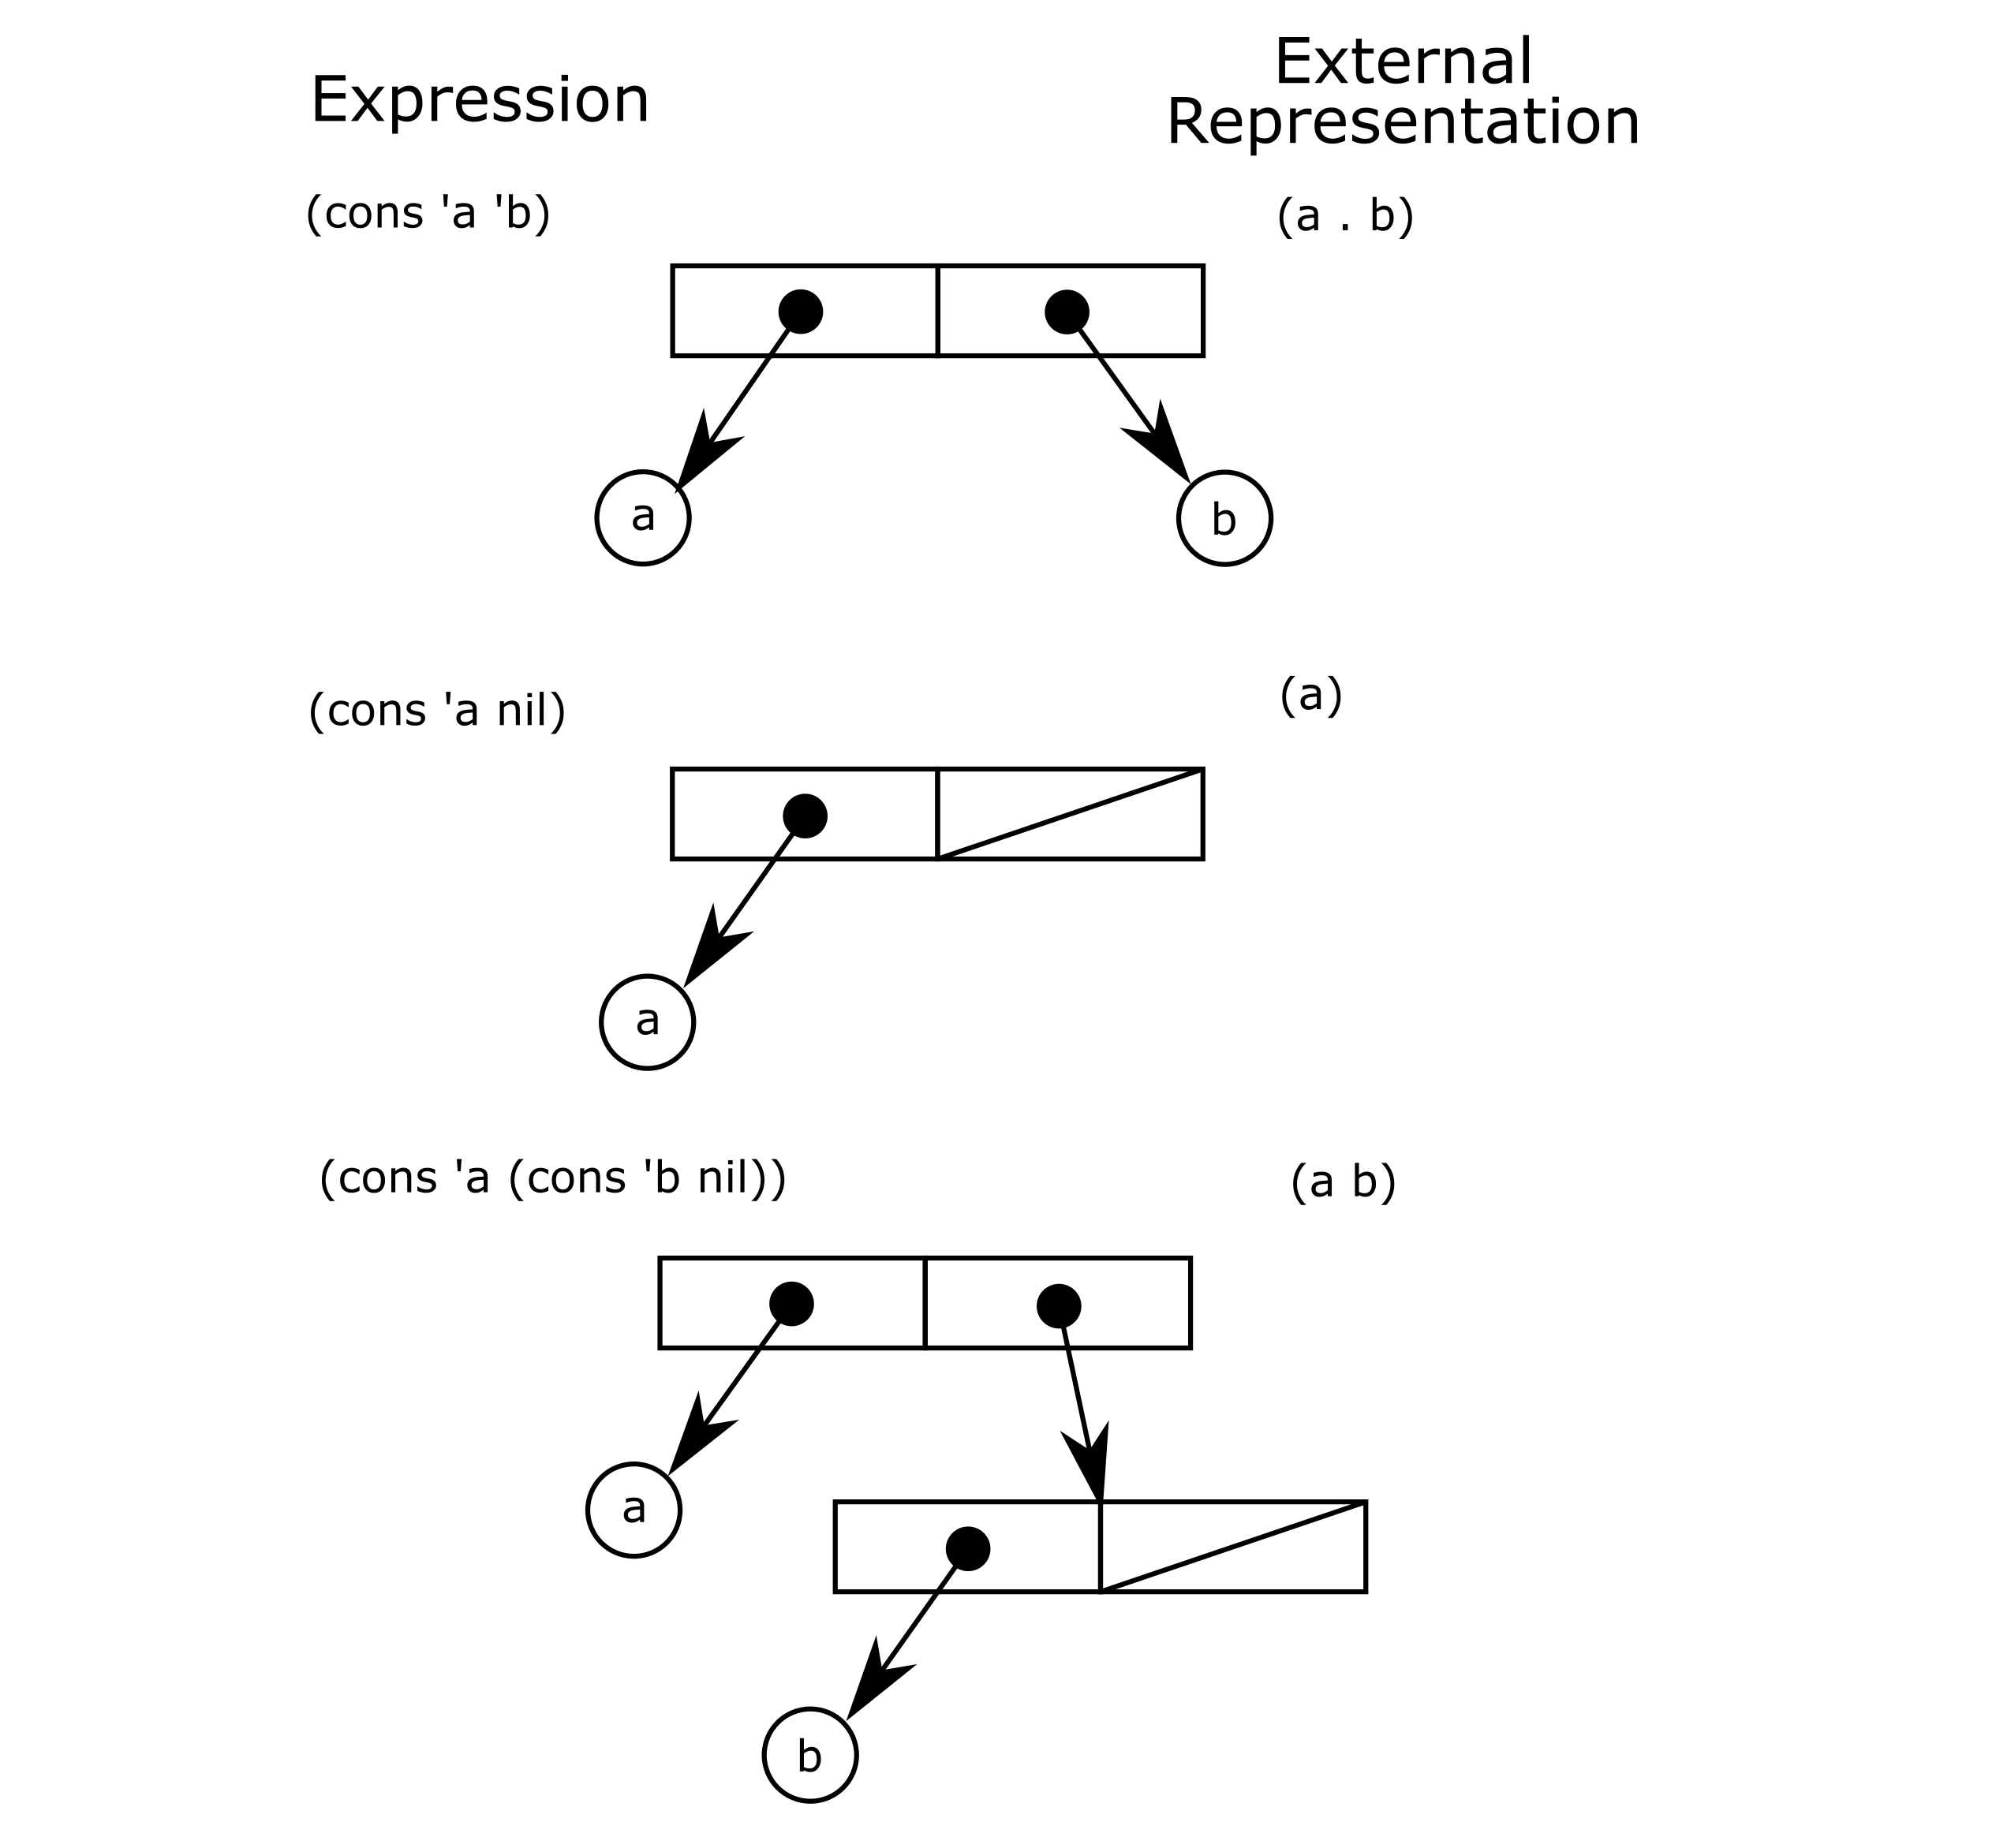
\includegraphics{images/consing.png}\captionsetup{labelformat=empty}\caption{ Examples of consing}\label{fig:-examples-of-consing}\end{figure}
\section{Unfinished code in file pairslists.ans line 201}
\noindent\begin{tabular}{ |p{1.9cm} p{8cm}| }
\hline
\rowcolor[HTML]{CCCCCC} \multicolumn{2}{|l|}{\bf cons (public)} \\
car & a Lisp value \\
cdr & a Lisp value \\
\textit{Returns:} & a pair \\
\hline
\end{tabular}
\section{Unfinished code in file pairslists.ans line 205}
\begin{lstlisting}
reg cons
\section{Unfinished code in file pairslists.ans line 208}
proc ::constcl::cons {car cdr} {
  MkPair $car $cdr
}
\end{lstlisting}
\section{Unfinished code in file pairslists.ans line 213}
\section{Unfinished code in file pairslists.ans line 215}
\section{Unfinished code in file pairslists.ans line 223}
\section{Unfinished code in file pairslists.ans line 225}
\subsection{car procedure}
\label{car-procedure}
\index{car procedure}
\section{Unfinished code in file pairslists.ans line 227}


\texttt{car} gets the contents of the first cell in a pair.

\section{Unfinished code in file pairslists.ans line 231}


Example:

\section{Unfinished code in file pairslists.ans line 235}
\begin{verbatim}
(car '(a b))   =>  a
\end{verbatim}
\section{Unfinished code in file pairslists.ans line 239}
\noindent\begin{tabular}{ |p{1.9cm} p{8cm}| }
\hline
\rowcolor[HTML]{CCCCCC} \multicolumn{2}{|l|}{\bf car (public)} \\
pair & a pair \\
\textit{Returns:} & a Lisp value \\
\hline
\end{tabular}
\section{Unfinished code in file pairslists.ans line 243}
\begin{lstlisting}
reg car
\section{Unfinished code in file pairslists.ans line 246}
proc ::constcl::car {pair} {
  $pair car
}
\end{lstlisting}
\section{Unfinished code in file pairslists.ans line 251}
\section{Unfinished code in file pairslists.ans line 253}
\section{Unfinished code in file pairslists.ans line 259}
\section{Unfinished code in file pairslists.ans line 263}
\section{Unfinished code in file pairslists.ans line 265}
\subsection{cdr procedure}
\label{cdr-procedure}
\index{cdr procedure}
\section{Unfinished code in file pairslists.ans line 267}


\texttt{cdr} gets the contents of the second cell in a pair.

\section{Unfinished code in file pairslists.ans line 271}


Example:

\section{Unfinished code in file pairslists.ans line 275}
\begin{verbatim}
(cdr '(a b))   =>  (b)
\end{verbatim}
\section{Unfinished code in file pairslists.ans line 279}
\noindent\begin{tabular}{ |p{1.9cm} p{8cm}| }
\hline
\rowcolor[HTML]{CCCCCC} \multicolumn{2}{|l|}{\bf cdr (public)} \\
pair & a pair \\
\textit{Returns:} & a Lisp value \\
\hline
\end{tabular}
\section{Unfinished code in file pairslists.ans line 283}
\begin{lstlisting}
reg cdr
\section{Unfinished code in file pairslists.ans line 286}
proc ::constcl::cdr {pair} {
  $pair cdr
}
\end{lstlisting}
\section{Unfinished code in file pairslists.ans line 291}
\section{Unfinished code in file pairslists.ans line 293}
\section{Unfinished code in file pairslists.ans line 298}
\section{Unfinished code in file pairslists.ans line 302}
\section{Unfinished code in file pairslists.ans line 304}

\section{Unfinished code in file pairslists.ans line 307}

\textbf{caar} to \textbf{cddddr} \texttt{car} and \texttt{cdr} can be combined to form 28 composite access operations.

\section{Unfinished code in file pairslists.ans line 311}
\index{caar}
\begin{lstlisting}
foreach ads {
  aa
  ad
  da
  dd
  aaa
  ada
  daa
  dda
  aad
  add
  dad
  ddd
  aaaa
  adaa
  daaa
  ddaa
  aada
  adda
  dada
  ddda
  aaad
  adad
  daad
  ddad
  aadd
  addd
  dadd
  dddd
} {
    reg c${ads}r
\section{Unfinished code in file pairslists.ans line 345}
    proc ::constcl::c${ads}r {pair} "
        foreach c \[lreverse \[split $ads {}\]\] {
            if {\$c eq \"a\"} {
                set pair \[car \$pair\]
            } else {
                set pair \[cdr \$pair\]
            }
        }
        return \$pair
    "
\section{Unfinished code in file pairslists.ans line 356}
}
\end{lstlisting}
\section{Unfinished code in file pairslists.ans line 359}
\subsection{set-car! procedure}
\label{set-car"!-procedure}
\index{set-car"! procedure}
\section{Unfinished code in file pairslists.ans line 361}


\texttt{set-car!} sets the contents of the first cell in a pair.

\section{Unfinished code in file pairslists.ans line 365}


Example:

\section{Unfinished code in file pairslists.ans line 369}
\begin{verbatim}
(let ((pair (cons 'a 'b)) (val 'x))
  (set-car! pair val))                =>  (x . b)
\end{verbatim}
\section{Unfinished code in file pairslists.ans line 374}
\noindent\begin{tabular}{ |p{1.9cm} p{8cm}| }
\hline
\rowcolor[HTML]{CCCCCC} \multicolumn{2}{|l|}{\bf set-car! (public)} \\
pair & a pair \\
val & a Lisp value \\
\textit{Returns:} & a pair \\
\hline
\end{tabular}
\section{Unfinished code in file pairslists.ans line 378}
\begin{lstlisting}
reg set-car!
\section{Unfinished code in file pairslists.ans line 381}
proc ::constcl::set-car! {pair val} {
  $pair set-car! $val
}
\end{lstlisting}
\section{Unfinished code in file pairslists.ans line 386}
\section{Unfinished code in file pairslists.ans line 388}
\section{Unfinished code in file pairslists.ans line 394}
\section{Unfinished code in file pairslists.ans line 398}
\section{Unfinished code in file pairslists.ans line 400}
\subsection{set-cdr! procedure}
\label{set-cdr"!-procedure}
\index{set-cdr"! procedure}
\section{Unfinished code in file pairslists.ans line 402}


\texttt{set-cdr!} sets the contents of the second cell in a pair.

\section{Unfinished code in file pairslists.ans line 406}


Example:

\section{Unfinished code in file pairslists.ans line 410}
\begin{verbatim}
(let ((pair (cons 'a 'b)) (val 'x))
  (set-cdr! pair val))                =>  (a . x)
\end{verbatim}
\section{Unfinished code in file pairslists.ans line 415}
\noindent\begin{tabular}{ |p{1.9cm} p{8cm}| }
\hline
\rowcolor[HTML]{CCCCCC} \multicolumn{2}{|l|}{\bf set-cdr! (public)} \\
pair & a pair \\
val & a Lisp value \\
\textit{Returns:} & a pair \\
\hline
\end{tabular}
\section{Unfinished code in file pairslists.ans line 419}
\begin{lstlisting}
reg set-cdr!
\section{Unfinished code in file pairslists.ans line 422}
proc ::constcl::set-cdr! {pair val} {
  $pair set-cdr! $val
}
\end{lstlisting}
\section{Unfinished code in file pairslists.ans line 427}
\section{Unfinished code in file pairslists.ans line 429}
\section{Unfinished code in file pairslists.ans line 435}
\section{Unfinished code in file pairslists.ans line 439}
\section{Unfinished code in file pairslists.ans line 441}
\subsection{list? procedure}
\label{list?-procedure}
\index{list? procedure}
\section{Unfinished code in file pairslists.ans line 443}


The \texttt{list?} predicate tests if a pair is part of a proper list, one that ends with NIL. See figure showing proper and improper lists (see page \pageref{fig:-a-proper-list-and-two-improper-ones}).

\section{Unfinished code in file pairslists.ans line 449}
\noindent\begin{tabular}{ |p{1.9cm} p{8cm}| }
\hline
\rowcolor[HTML]{CCCCCC} \multicolumn{2}{|l|}{\bf list? (public)} \\
val & a Lisp value \\
\textit{Returns:} & a boolean \\
\hline
\end{tabular}
\section{Unfinished code in file pairslists.ans line 453}
\begin{lstlisting}
reg list?
\section{Unfinished code in file pairslists.ans line 456}
proc ::constcl::list? {val} {
  set visited {}
  if {[T [null? $val]]} {
      return #t
  } elseif {[T [pair? $val]]} {
      return [listp $val]
  } else {
      return #f
  }
}
\end{lstlisting}
\section{Unfinished code in file pairslists.ans line 468}

\section{Unfinished code in file pairslists.ans line 471}

\textbf{listp} procedure \texttt{listp} is a helper procedure that recursively traverses a cons trail to find out if it is cyclic or ends in an atom, which means that the procedure returns false, or if it ends in \texttt{\#NIL}, which means that it returns true.

\section{Unfinished code in file pairslists.ans line 476}
\noindent\begin{tabular}{ |p{1.9cm} p{8cm}| }
\hline
\rowcolor[HTML]{CCCCCC} \multicolumn{2}{|l|}{\bf listp (internal)} \\
pair & a pair \\
\textit{Returns:} & a boolean \\
\hline
\end{tabular}
\section{Unfinished code in file pairslists.ans line 480}
\index{listp}
\begin{lstlisting}
proc ::constcl::listp {pair} {
  upvar visited visited
  if {$pair in $visited} {
    return #f
  }
  lappend visited $pair
  if {[T [null? $pair]]} {
    return #t
  } elseif {[T [pair? $pair]]} {
    return [listp [cdr $pair]]
  } else {
    return #f
  }
}
\end{lstlisting}
\section{Unfinished code in file pairslists.ans line 498}
\section{Unfinished code in file pairslists.ans line 500}
\section{Unfinished code in file pairslists.ans line 507}
\section{Unfinished code in file pairslists.ans line 514}
\section{Unfinished code in file pairslists.ans line 516}
\subsection{list procedure}
\label{list-procedure}
\index{list procedure}
\section{Unfinished code in file pairslists.ans line 518}


\texttt{list} constructs a Lisp list from a number of values.

\section{Unfinished code in file pairslists.ans line 522}


Example:

\section{Unfinished code in file pairslists.ans line 526}
\begin{verbatim}
(list 1 2 3)   =>  (1 2 3)
\end{verbatim}
\section{Unfinished code in file pairslists.ans line 530}
\noindent\begin{tabular}{ |p{1.9cm} p{8cm}| }
\hline
\rowcolor[HTML]{CCCCCC} \multicolumn{2}{|l|}{\bf list (public)} \\
args & some Lisp values \\
\textit{Returns:} & a Lisp list of Lisp values \\
\hline
\end{tabular}
\section{Unfinished code in file pairslists.ans line 534}
\begin{lstlisting}
reg list
\section{Unfinished code in file pairslists.ans line 537}
proc ::constcl::list {args} {
  if {[llength $args] == 0} {
    return #NIL
  } else {
    set prev #NIL
    foreach obj [lreverse $args] {
      set prev [cons $obj $prev]
    }
    return $prev
  }
}
\end{lstlisting}
\section{Unfinished code in file pairslists.ans line 550}
\section{Unfinished code in file pairslists.ans line 552}
\section{Unfinished code in file pairslists.ans line 557}
\section{Unfinished code in file pairslists.ans line 559}
\subsection{length procedure}
\label{length-procedure}
\index{length procedure}
\section{Unfinished code in file pairslists.ans line 561}


\texttt{length} reports the length of a Lisp list.

\section{Unfinished code in file pairslists.ans line 565}


Example:

\section{Unfinished code in file pairslists.ans line 569}
\begin{verbatim}
(length '(a b c d))   =>  4
\end{verbatim}
\section{Unfinished code in file pairslists.ans line 573}
\noindent\begin{tabular}{ |p{1.9cm} p{8cm}| }
\hline
\rowcolor[HTML]{CCCCCC} \multicolumn{2}{|l|}{\bf length (public)} \\
pair & a pair \\
\textit{Returns:} & a number \\
\hline
\end{tabular}
\section{Unfinished code in file pairslists.ans line 577}
\begin{lstlisting}
reg length
\section{Unfinished code in file pairslists.ans line 580}
proc ::constcl::length {pair} {
  check {list? $pair} {
    LIST expected\n([pn] lst)
  }
  MkNumber [length-helper $pair]
}
\end{lstlisting}
\section{Unfinished code in file pairslists.ans line 588}

\section{Unfinished code in file pairslists.ans line 591}

\textbf{length-helper} procedure \texttt{length-helper} is a helper procedure which measures a list recursively.

\section{Unfinished code in file pairslists.ans line 594}
\noindent\begin{tabular}{ |p{1.9cm} p{8cm}| }
\hline
\rowcolor[HTML]{CCCCCC} \multicolumn{2}{|l|}{\bf length-helper (internal)} \\
pair & a pair \\
\textit{Returns:} & a Tcl number \\
\hline
\end{tabular}
\section{Unfinished code in file pairslists.ans line 598}
\index{length-helper}
\begin{lstlisting}
proc ::constcl::length-helper {pair} {
  if {[T [null? $pair]]} {
    return 0
  } else {
    return [expr {1 +
      [length-helper [cdr $pair]]}]
  }
}
\end{lstlisting}
\section{Unfinished code in file pairslists.ans line 610}
\section{Unfinished code in file pairslists.ans line 612}
\section{Unfinished code in file pairslists.ans line 618}
\section{Unfinished code in file pairslists.ans line 620}
\subsection{append procedure}
\label{append-procedure}
\index{append procedure}
\section{Unfinished code in file pairslists.ans line 622}


\texttt{append} joins lists together.

\section{Unfinished code in file pairslists.ans line 626}


Example:

\section{Unfinished code in file pairslists.ans line 630}
\begin{verbatim}
(append '(a b) '(c d))   =>  (a b c d)
\end{verbatim}
\section{Unfinished code in file pairslists.ans line 634}
\noindent\begin{tabular}{ |p{1.9cm} p{8cm}| }
\hline
\rowcolor[HTML]{CCCCCC} \multicolumn{2}{|l|}{\bf append (public)} \\
args & some lists \\
\textit{Returns:} & a Lisp list of Lisp values \\
\hline
\end{tabular}
\section{Unfinished code in file pairslists.ans line 638}
\begin{lstlisting}
reg append
\section{Unfinished code in file pairslists.ans line 641}
proc ::constcl::append {args} {
  set prev [lindex $args end]
  foreach r [lreverse [lrange $args 0 end-1]] {
    check {list? $r} {
      LIST expected\n([pn] [$r show])
    }
    set prev [copy-list $r $prev]
  }
  set prev
}
\end{lstlisting}
\section{Unfinished code in file pairslists.ans line 653}

\section{Unfinished code in file pairslists.ans line 656}

\textbf{copy-list} procedure \texttt{copy-list} joins together two lists by recursively consing items from the first list towards the second.

\section{Unfinished code in file pairslists.ans line 660}
\noindent\begin{tabular}{ |p{1.9cm} p{8cm}| }
\hline
\rowcolor[HTML]{CCCCCC} \multicolumn{2}{|l|}{\bf copy-list (internal)} \\
pair & a pair \\
next & a Lisp list of Lisp values \\
\textit{Returns:} & a Lisp list of Lisp values \\
\hline
\end{tabular}
\section{Unfinished code in file pairslists.ans line 664}
\index{copy-list}
\begin{lstlisting}
proc ::constcl::copy-list {pair next} {
  # TODO only fresh conses in the direct chain to NIL
  if {[T [null? $pair]]} {
    set next
  } elseif {[T [null? [cdr $pair]]]} {
    cons [car $pair] $next
  } else {
    cons [car $pair] [copy-list [cdr $pair] $next]
  }
}
\end{lstlisting}
\section{Unfinished code in file pairslists.ans line 678}
\section{Unfinished code in file pairslists.ans line 688}
\section{Unfinished code in file pairslists.ans line 692}
\section{Unfinished code in file pairslists.ans line 694}
\subsection{reverse procedure}
\label{reverse-procedure}
\index{reverse procedure}
\section{Unfinished code in file pairslists.ans line 696}


\texttt{reverse} produces a reversed copy of a Lisp list.

\section{Unfinished code in file pairslists.ans line 700}


Example:

\section{Unfinished code in file pairslists.ans line 704}
\begin{verbatim}
(reverse '(a b c))   =>  (c b a)
\end{verbatim}
\section{Unfinished code in file pairslists.ans line 708}
\noindent\begin{tabular}{ |p{1.9cm} p{8cm}| }
\hline
\rowcolor[HTML]{CCCCCC} \multicolumn{2}{|l|}{\bf reverse (public)} \\
vals & a Lisp list of Lisp values \\
\textit{Returns:} & a Lisp list of Lisp values \\
\hline
\end{tabular}
\section{Unfinished code in file pairslists.ans line 712}
\begin{lstlisting}
reg reverse
\section{Unfinished code in file pairslists.ans line 715}
proc ::constcl::reverse {vals} {
  list {*}[lreverse [splitlist $vals]]
}
\end{lstlisting}
\section{Unfinished code in file pairslists.ans line 720}
\section{Unfinished code in file pairslists.ans line 722}
\section{Unfinished code in file pairslists.ans line 727}
\section{Unfinished code in file pairslists.ans line 729}
\subsection{list-tail procedure}
\label{list-tail-procedure}
\index{list-tail procedure}
\section{Unfinished code in file pairslists.ans line 731}


Given a list index, \texttt{list-tail} yields the sublist starting from that index.

\section{Unfinished code in file pairslists.ans line 735}


Example:

\section{Unfinished code in file pairslists.ans line 739}
\begin{verbatim}
(let ((lst '(a b c d e f)) (k 3))
  (list-tail lst k))                =>  (d e f)
\end{verbatim}
\section{Unfinished code in file pairslists.ans line 744}
\noindent\begin{tabular}{ |p{1.9cm} p{8cm}| }
\hline
\rowcolor[HTML]{CCCCCC} \multicolumn{2}{|l|}{\bf list-tail (public)} \\
vals & a Lisp list of Lisp values \\
k & a number \\
\textit{Returns:} & a Lisp list of Lisp values \\
\hline
\end{tabular}
\section{Unfinished code in file pairslists.ans line 748}
\begin{lstlisting}
reg list-tail
\section{Unfinished code in file pairslists.ans line 751}
proc ::constcl::list-tail {vals k} {
  if {[T [zero? $k]]} {
    return $vals
  } else {
    list-tail [cdr $vals] [- $k #1]
  }
}
\end{lstlisting}
\section{Unfinished code in file pairslists.ans line 760}
\section{Unfinished code in file pairslists.ans line 762}
\section{Unfinished code in file pairslists.ans line 766}
\section{Unfinished code in file pairslists.ans line 768}
\subsection{list-ref procedure}
\label{list-ref-procedure}
\index{list-ref procedure}
\section{Unfinished code in file pairslists.ans line 770}


\texttt{list-ref} yields the list item at a given index.

\section{Unfinished code in file pairslists.ans line 774}


Example:

\section{Unfinished code in file pairslists.ans line 778}
\begin{verbatim}
(let ((lst '(a b c d e f)) (k 3))
  (list-ref lst k))                 =>  d
\end{verbatim}
\section{Unfinished code in file pairslists.ans line 783}
\noindent\begin{tabular}{ |p{1.9cm} p{8cm}| }
\hline
\rowcolor[HTML]{CCCCCC} \multicolumn{2}{|l|}{\bf list-ref (public)} \\
vals & a Lisp list of Lisp values \\
k & a number \\
\textit{Returns:} & a Lisp value \\
\hline
\end{tabular}
\section{Unfinished code in file pairslists.ans line 787}
\begin{lstlisting}
reg list-ref
\section{Unfinished code in file pairslists.ans line 790}
proc ::constcl::list-ref {vals k} {
  car [list-tail $vals $k]
}
\end{lstlisting}
\section{Unfinished code in file pairslists.ans line 795}
\section{Unfinished code in file pairslists.ans line 797}
\section{Unfinished code in file pairslists.ans line 801}
\section{Unfinished code in file pairslists.ans line 803}
\subsection{memq procedure}
\label{memq-procedure}
\index{memq procedure}
\section{Unfinished code in file pairslists.ans line 805}

\noindent \textbf{memv} procedure

\section{Unfinished code in file pairslists.ans line 807}

\noindent \textbf{member} procedure

\section{Unfinished code in file pairslists.ans line 809}


\texttt{memq}, \texttt{memv}, and \texttt{member} return the sublist starting with a given item, or \texttt{\#f} if there is none. They use \texttt{eq?}, \texttt{eqv?}, and \texttt{equal?}, respectively, for the comparison.

\section{Unfinished code in file pairslists.ans line 815}


Example:

\section{Unfinished code in file pairslists.ans line 819}
\begin{verbatim}
(let ((lst '(a b c d e f)) (val 'd))
  (memq val lst))                      =>  (d e f)
\end{verbatim}
\section{Unfinished code in file pairslists.ans line 824}
\noindent\begin{tabular}{ |p{1.9cm} p{8cm}| }
\hline
\rowcolor[HTML]{CCCCCC} \multicolumn{2}{|l|}{\bf memq (public)} \\
val1 & a Lisp value \\
val2 & a Lisp list of Lisp values \\
\textit{Returns:} & a Lisp list of values OR \#f \\
\hline
\end{tabular}
\section{Unfinished code in file pairslists.ans line 828}
\begin{lstlisting}
reg memq
\section{Unfinished code in file pairslists.ans line 831}
proc ::constcl::memq {val1 val2} {
  return [member-proc eq? $val1 $val2]
}
\end{lstlisting}
\section{Unfinished code in file pairslists.ans line 836}
\section{Unfinished code in file pairslists.ans line 838}
\section{Unfinished code in file pairslists.ans line 847}
\section{Unfinished code in file pairslists.ans line 851}
\section{Unfinished code in file pairslists.ans line 853}
\noindent\begin{tabular}{ |p{1.9cm} p{8cm}| }
\hline
\rowcolor[HTML]{CCCCCC} \multicolumn{2}{|l|}{\bf memv (public)} \\
val1 & a Lisp value \\
val2 & a Lisp list of Lisp values \\
\textit{Returns:} & a Lisp list of values OR \#f \\
\hline
\end{tabular}
\section{Unfinished code in file pairslists.ans line 857}
\index{memv}
\begin{lstlisting}
reg memv
\section{Unfinished code in file pairslists.ans line 861}
proc ::constcl::memv {val1 val2} {
  return [member-proc eqv? $val1 $val2]
}
\end{lstlisting}
\section{Unfinished code in file pairslists.ans line 866}
\noindent\begin{tabular}{ |p{1.9cm} p{8cm}| }
\hline
\rowcolor[HTML]{CCCCCC} \multicolumn{2}{|l|}{\bf member (public)} \\
val1 & a Lisp value \\
val2 & a Lisp list of Lisp values \\
\textit{Returns:} & a Lisp list of values OR \#f \\
\hline
\end{tabular}
\section{Unfinished code in file pairslists.ans line 870}
\index{member}
\begin{lstlisting}
reg member
\section{Unfinished code in file pairslists.ans line 874}
proc ::constcl::member {val1 val2} {
  return [member-proc equal? $val1 $val2]
}
\end{lstlisting}
\section{Unfinished code in file pairslists.ans line 879}

\section{Unfinished code in file pairslists.ans line 882}

\textbf{member-proc} procedure The \texttt{member-proc} helper procedure does the work for the \texttt{memq}, \texttt{memv}, and \texttt{member} procedures. It works by comparing against the \texttt{car} of the list, then recursively taking the \texttt{cdr} of the list.

\section{Unfinished code in file pairslists.ans line 887}
\noindent\begin{tabular}{ |p{1.9cm} p{8cm}| }
\hline
\rowcolor[HTML]{CCCCCC} \multicolumn{2}{|l|}{\bf member-proc (internal)} \\
epred & an equivalence predicate \\
val1 & a Lisp value \\
val2 & a Lisp list of Lisp values \\
\textit{Returns:} & a Lisp list of values OR \#f \\
\hline
\end{tabular}
\section{Unfinished code in file pairslists.ans line 891}
\index{member-proc}
\begin{lstlisting}
proc ::constcl::member-proc {epred val1 val2} {
  switch $epred {
    eq? { set name "memq" }
    eqv? { set name "memv" }
    equal? { set name "member" }
  }
  check {list? $val2} {
    LIST expected\n($name [$val1 show] [$val2 show])
  }
  if {[T [null? $val2]]} {
    return #f
  } elseif {[T [pair? $val2]]} {
    if {[T [$epred $val1 [car $val2]]]} {
      return $val2
    } else {
      return [member-proc $epred $val1 [cdr $val2]]
    }
  }
}
\end{lstlisting}
\section{Unfinished code in file pairslists.ans line 914}
\subsection{assq procedure}
\label{assq-procedure}
\index{assq procedure}
\section{Unfinished code in file pairslists.ans line 916}

\noindent \textbf{assv} procedure

\section{Unfinished code in file pairslists.ans line 918}

\noindent \textbf{assoc} procedure

\section{Unfinished code in file pairslists.ans line 920}

\section{Unfinished code in file pairslists.ans line 926}

\texttt{assq}, \texttt{assv}, and \texttt{assoc} scan an association list and return the association pair with a given key, or \texttt{\#f} if there is none. They use \texttt{eq?}, \texttt{eqv?}, and \texttt{equal?}, respectively, for the comparison. They implement lookup in the kind of lookup table known as an association list, or \emph{alist}. Example:

\section{Unfinished code in file pairslists.ans line 929}
\begin{verbatim}
(let ((e '((a . 1) (b . 2) (c . 3))) (key 'a))
  (assq key e))                                  => (a . 1)
\end{verbatim}
\section{Unfinished code in file pairslists.ans line 934}
\noindent\begin{tabular}{ |p{1.9cm} p{8cm}| }
\hline
\rowcolor[HTML]{CCCCCC} \multicolumn{2}{|l|}{\bf assq (public)} \\
val1 & a Lisp value \\
val2 & an association list \\
\textit{Returns:} & an association pair or \#f \\
\hline
\end{tabular}
\section{Unfinished code in file pairslists.ans line 938}
\begin{lstlisting}
reg assq
\section{Unfinished code in file pairslists.ans line 941}
proc ::constcl::assq {val1 val2} {
  return [assoc-proc eq? $val1 $val2]
}
\end{lstlisting}
\section{Unfinished code in file pairslists.ans line 946}
\noindent\begin{tabular}{ |p{1.9cm} p{8cm}| }
\hline
\rowcolor[HTML]{CCCCCC} \multicolumn{2}{|l|}{\bf assv (public)} \\
val1 & a Lisp value \\
val2 & an association list \\
\textit{Returns:} & an association pair or \#f \\
\hline
\end{tabular}
\section{Unfinished code in file pairslists.ans line 950}
\section{Unfinished code in file pairslists.ans line 951}
\index{assv}
\begin{lstlisting}
reg assv
\section{Unfinished code in file pairslists.ans line 955}
proc ::constcl::assv {val1 val2} {
  return [assoc-proc eqv? $val1 $val2]
}
\end{lstlisting}
\section{Unfinished code in file pairslists.ans line 960}
\noindent\begin{tabular}{ |p{1.9cm} p{8cm}| }
\hline
\rowcolor[HTML]{CCCCCC} \multicolumn{2}{|l|}{\bf assoc (public)} \\
val1 & a Lisp value \\
val2 & an association list \\
\textit{Returns:} & an association pair or \#f \\
\hline
\end{tabular}
\section{Unfinished code in file pairslists.ans line 964}
\section{Unfinished code in file pairslists.ans line 965}
\index{assoc}
\begin{lstlisting}
reg assoc
\section{Unfinished code in file pairslists.ans line 969}
proc ::constcl::assoc {val1 val2} {
  return [assoc-proc equal? $val1 $val2]
}
\end{lstlisting}
\section{Unfinished code in file pairslists.ans line 974}

\section{Unfinished code in file pairslists.ans line 977}

\textbf{assoc-proc} procedure \texttt{assoc-proc} is a helper procedure which does the work for \texttt{assq}, \texttt{assv}, and \texttt{assoc}.

\section{Unfinished code in file pairslists.ans line 981}
\noindent\begin{tabular}{ |p{1.9cm} p{8cm}| }
\hline
\rowcolor[HTML]{CCCCCC} \multicolumn{2}{|l|}{\bf assoc-proc (internal)} \\
epred & an equivalence predicate \\
val1 & a Lisp value \\
val2 & an association list \\
\textit{Returns:} & an association pair or \#f \\
\hline
\end{tabular}
\section{Unfinished code in file pairslists.ans line 985}
\index{assoc-proc}
\begin{lstlisting}
proc ::constcl::assoc-proc {epred val1 val2} {
  switch $epred {
    eq? { set name "assq" }
    eqv? { set name "assv" }
    equal? { set name "assoc" }
  }
  check {list? $val2} {
    LIST expected\n($name [$val1 show] [$val2 show])
  }
  if {[T [null? $val2]]} {
    return #f
  } elseif {[T [pair? $val2]]} {
    if {[T [pair? [car $val2]]] && 
      [T [$epred $val1 [caar $val2]]]} {
      return [car $val2]
    } else {
      return [assoc-proc $epred $val1 [cdr $val2]]
    }
  }
}
\end{lstlisting}
\section{Unfinished code in file pairslists.ans line 1009}
\section{Unfinished code in file pairslists.ans line 1022}
\section{Unfinished code in file strings.ans line 3}
\section{Strings}
\label{strings}
\index{Strings}
\section{Unfinished code in file strings.ans line 5}


Procedures for dealing with strings of characters.

\section{Unfinished code in file strings.ans line 9}
\subsection{String class}
\label{string-class}
\index{String class}
\section{Unfinished code in file strings.ans line 11}

\section{Unfinished code in file strings.ans line 17}

Strings have the internal representation of a vector of character objects, with the data elements of 1) the vector address of the first element, and 2) the length of the vector. External representation is surrounded by double quotes, with double quotes and backslashes within the string escaped with a backslash. As a ConsTcl extension, a \texttt{\textbackslash n} pair in the external representation is stored as a newline character. It is restored to \texttt{\textbackslash n} if the string is printed using \texttt{write}, but remains a newline character if the string is printed with \texttt{display}.

\section{Unfinished code in file strings.ans line 23}
\begin{lstlisting}
oo::class create ::constcl::String {
  superclass ::constcl::NIL
  variable data constant
  constructor {v} {
    set v [::string trim $v "\""]
    set v [string map {\\\\ \\ \\\" \" \\n \n} $v]
    set len [::string length $v]
    set vsa [::constcl::vsAlloc $len]
    set idx $vsa
    foreach elt [split $v {}] {
      if {$elt eq " "} {
        set c #\\space
      } elseif {$elt eq "\n"} {
        set c #\\newline
      } else {
        set c #\\$elt
      }
      lset ::constcl::vectorSpace $idx \
        [::constcl::MkChar $c]
      incr idx
    }
    set data [
      ::constcl::cons [N $vsa] [N $len]]
    set constant 0
  }
  method = {str} {
    ::string equal [my value] [$str value]
  }
  method cmp {str} {
    ::string compare [my value] [$str value]
  }
  method length {} {
    ::constcl::cdr $data
  }
  method ref {k} {
    set k [$k numval]
    if {$k < 0 || $k >= [[my length] numval]} {
      ::error "index out of range\n$k"
    }
    lindex [my store] $k
  }
  method store {} {
    set base [[::constcl::car $data] numval]
    set end [expr {[[my length] numval] +
      $base - 1}]
    lrange $::constcl::vectorSpace $base $end
  }
  method value {} {
    join [lmap c [my store] {$c char}] {}
  }
  method set! {k c} {
    if {[my constant]} {
      ::error "string is constant"
    } else {
      set k [$k numval]
      if {$k < 0 ||
        $k >= [[my length] numval]} {
        ::error "index out of range\n$k"
      }
      set base [[::constcl::car $data] numval]
      lset ::constcl::vectorSpace $k+$base $c
    }
    return [self]
  }
  method fill! {c} {
    if {[my constant]} {
      ::error "string is constant"
    } else {
      set base [[::constcl::car $data] numval]
      set len [[my length] numval]
      for {set idx $base} \
        {$idx < $len+$base} \
        {incr idx} {
        lset ::constcl::vectorSpace $idx $c
      }
    }
    return [self]
  }
  method substring {from to} {
    join [lmap c [lrange [my store] \
      [$from numval] [$to numval]] {$c char}] {}
  }
  method mkconstant {} {
    set constant 1
  }
  method constant {} {
    set constant
  }
  method external {} {
    return "\"[
      string map {\\ \\\\ \" \\\" \n \\n} [my value]]\""
  }
  method write {handle} {
    puts -nonewline $handle [my external]
  }
  method display {handle} {
    puts -nonewline $handle [my value]
  }
  method show {} {
    my external
  }
}
\end{lstlisting}
\section{Unfinished code in file strings.ans line 128}
\subsection{MkString generator}
\label{mkstring-generator}
\index{MkString generator}
\section{Unfinished code in file strings.ans line 130}


\texttt{MkString} generates a String object.

\section{Unfinished code in file strings.ans line 134}
\noindent\begin{tabular}{ |p{1.9cm} p{8cm}| }
\hline
\rowcolor[HTML]{CCCCCC} \multicolumn{2}{|l|}{\bf MkString (internal)} \\
str & an external rep of a string \\
\textit{Returns:} & a string \\
\hline
\end{tabular}
\section{Unfinished code in file strings.ans line 138}
\begin{lstlisting}
interp alias {} ::constcl::MkString \
  {} ::constcl::String new
\end{lstlisting}
\section{Unfinished code in file strings.ans line 143}
\section{Unfinished code in file strings.ans line 150}
\section{Unfinished code in file strings.ans line 157}
\section{Unfinished code in file strings.ans line 163}
\subsection{string? procedure}
\label{string?-procedure}
\index{string? procedure}
\section{Unfinished code in file strings.ans line 165}


\texttt{string?} recognizes a string by type.

\section{Unfinished code in file strings.ans line 169}
\noindent\begin{tabular}{ |p{1.9cm} p{8cm}| }
\hline
\rowcolor[HTML]{CCCCCC} \multicolumn{2}{|l|}{\bf string? (public)} \\
val & a Lisp value \\
\textit{Returns:} & a boolean \\
\hline
\end{tabular}
\section{Unfinished code in file strings.ans line 173}
\begin{lstlisting}
reg string?
\section{Unfinished code in file strings.ans line 176}
proc ::constcl::string? {val} {
  typeof? $val String
}
\end{lstlisting}
\section{Unfinished code in file strings.ans line 181}
\section{Unfinished code in file strings.ans line 183}
\section{Unfinished code in file strings.ans line 188}
\section{Unfinished code in file strings.ans line 190}
\subsection{make-string procedure}
\label{make-string-procedure}
\index{make-string procedure}
\section{Unfinished code in file strings.ans line 192}


\texttt{make-string} creates a string of \emph{k} characters, optionally filled with \emph{char} characters. If \emph{char} is omitted, the string will be filled with space characters.

\section{Unfinished code in file strings.ans line 197}


Example:

\section{Unfinished code in file strings.ans line 201}
\begin{verbatim}
(let ((k 5))
  (make-string k))        =>  "     "
(let ((k 5) (char #\A))
  (make-string k char))   =>  "AAAAA"
\end{verbatim}
\section{Unfinished code in file strings.ans line 208}
\noindent\begin{tabular}{ |p{1.9cm} p{8cm}| }
\hline
\rowcolor[HTML]{CCCCCC} \multicolumn{2}{|l|}{\bf make-string (public)} \\
k & a number \\
?char? & a character \\
\textit{Returns:} & a string \\
\hline
\end{tabular}
\section{Unfinished code in file strings.ans line 212}
\begin{lstlisting}
reg make-string
\section{Unfinished code in file strings.ans line 215}
proc ::constcl::make-string {k args} {
  set i [$k numval]
  if {[llength $args] == 0} {
    set char " "
  } else {
    lassign $args c
    set char [$c char]
  }
  return [MkString [::string repeat $char $i]]
}
\end{lstlisting}
\section{Unfinished code in file strings.ans line 227}
\section{Unfinished code in file strings.ans line 229}
\section{Unfinished code in file strings.ans line 233}
\section{Unfinished code in file strings.ans line 235}
\subsection{string procedure}
\label{string-procedure}
\index{string procedure}
\section{Unfinished code in file strings.ans line 237}


\texttt{string} constructs a string from a number of Lisp characters.

\section{Unfinished code in file strings.ans line 241}


Example:

\section{Unfinished code in file strings.ans line 245}
\begin{verbatim}
(string #\f #\o #\o)   =>  "foo"
\end{verbatim}
\section{Unfinished code in file strings.ans line 249}
\noindent\begin{tabular}{ |p{1.9cm} p{8cm}| }
\hline
\rowcolor[HTML]{CCCCCC} \multicolumn{2}{|l|}{\bf string (public)} \\
args & some characters \\
\textit{Returns:} & a string \\
\hline
\end{tabular}
\section{Unfinished code in file strings.ans line 253}
\begin{lstlisting}
reg string
\section{Unfinished code in file strings.ans line 256}
proc ::constcl::string {args} {
  set str {}
  foreach char $args {
    check {::constcl::char? $char} {
      CHAR expected\n([pn] [lmap c $args \
        {$c show}])
    }
    ::append str [$char char]
  }
  return [MkString $str]
}
\end{lstlisting}
\section{Unfinished code in file strings.ans line 269}
\section{Unfinished code in file strings.ans line 271}
\section{Unfinished code in file strings.ans line 275}
\section{Unfinished code in file strings.ans line 279}
\section{Unfinished code in file strings.ans line 281}
\subsection{string-length procedure}
\label{string-length-procedure}
\index{string-length procedure}
\section{Unfinished code in file strings.ans line 283}


\texttt{string-length} reports a string's length.

\section{Unfinished code in file strings.ans line 287}


Example:

\section{Unfinished code in file strings.ans line 291}
\begin{verbatim}
(string-length "foobar")   => 6
\end{verbatim}
\section{Unfinished code in file strings.ans line 295}
\noindent\begin{tabular}{ |p{1.9cm} p{8cm}| }
\hline
\rowcolor[HTML]{CCCCCC} \multicolumn{2}{|l|}{\bf string-length (public)} \\
str & a string \\
\textit{Returns:} & a number \\
\hline
\end{tabular}
\section{Unfinished code in file strings.ans line 299}
\begin{lstlisting}
reg string-length
\section{Unfinished code in file strings.ans line 302}
proc ::constcl::string-length {str} {
  check {::constcl::string? $str} {
    STRING expected\n([pn] [$str show])
  }
  return [$str length]
}
\end{lstlisting}
\section{Unfinished code in file strings.ans line 310}
\section{Unfinished code in file strings.ans line 312}
\section{Unfinished code in file strings.ans line 316}
\section{Unfinished code in file strings.ans line 318}
\subsection{string-ref procedure}
\label{string-ref-procedure}
\index{string-ref procedure}
\section{Unfinished code in file strings.ans line 320}


\texttt{string-ref} yields the \emph{k}-th character (0-based) in \emph{str}.

\section{Unfinished code in file strings.ans line 324}


Example:

\section{Unfinished code in file strings.ans line 328}
\begin{verbatim}
(string-ref "foobar" 3)   => #\b
\end{verbatim}
\section{Unfinished code in file strings.ans line 332}
\noindent\begin{tabular}{ |p{1.9cm} p{8cm}| }
\hline
\rowcolor[HTML]{CCCCCC} \multicolumn{2}{|l|}{\bf string-ref (public)} \\
str & a string \\
k & a number \\
\textit{Returns:} & a character \\
\hline
\end{tabular}
\section{Unfinished code in file strings.ans line 336}
\begin{lstlisting}
reg string-ref
\section{Unfinished code in file strings.ans line 339}
proc ::constcl::string-ref {str k} {
  check {::constcl::string? $str} {
    STRING expected\n([pn] [$str show] \
      [$k show])
  }
  check {::constcl::number? $k} {
    INTEGER expected\n([pn] [$str show] \
      [$k show])
  }
  return [$str ref $k]
}
\end{lstlisting}
\section{Unfinished code in file strings.ans line 352}
\section{Unfinished code in file strings.ans line 354}
\section{Unfinished code in file strings.ans line 358}
\section{Unfinished code in file strings.ans line 360}
\subsection{string-set! procedure}
\label{string-set"!-procedure}
\index{string-set"! procedure}
\section{Unfinished code in file strings.ans line 362}


\texttt{string-set!} replaces the character at \emph{k} with \emph{char} in a non-constant string.

\section{Unfinished code in file strings.ans line 366}


Example:

\section{Unfinished code in file strings.ans line 370}
\begin{verbatim}
(let ((str (string #\f #\o #\o))
      (k 2)
      (char #\x))
  (string-set! str k char))         =>  "fox"
\end{verbatim}
\section{Unfinished code in file strings.ans line 377}
\noindent\begin{tabular}{ |p{1.9cm} p{8cm}| }
\hline
\rowcolor[HTML]{CCCCCC} \multicolumn{2}{|l|}{\bf string-set! (public)} \\
str & a string \\
k & a number \\
char & a character \\
\textit{Returns:} & a string \\
\hline
\end{tabular}
\section{Unfinished code in file strings.ans line 381}
\begin{lstlisting}
reg string-set!
\section{Unfinished code in file strings.ans line 384}
proc ::constcl::string-set! {str k char} {
  check {string? $str} {
    STRING expected\n([pn] [$str show] [$k show] \
      [$char show])
  }
  check {number? $k} {
    INTEGER expected\n([pn] [$str show] \
      [$k show] [$char show])
  }
  check {char? $char} {
    CHAR expected\n([pn] [$str show] [$k show] \
      [$char show])
  }
  $str set! $k $char
  return $str
}
\end{lstlisting}
\section{Unfinished code in file strings.ans line 402}
\section{Unfinished code in file strings.ans line 404}
\section{Unfinished code in file strings.ans line 408}
\section{Unfinished code in file strings.ans line 414}
\section{Unfinished code in file strings.ans line 418}
\section{Unfinished code in file strings.ans line 420}

\section{Unfinished code in file strings.ans line 423}
\section{Unfinished code in file strings.ans line 425}
\section{Unfinished code in file strings.ans line 427}
\section{Unfinished code in file strings.ans line 429}
\section{Unfinished code in file strings.ans line 431}

\textbf{string=?}, \textbf{string-ci=?} \textbf{string<?}, \textbf{string-ci<?} \textbf{string>?}, \textbf{string-ci>?} \textbf{string<=?}, \textbf{string-ci<=?} \textbf{string>=?}, \textbf{string-ci>=?} \texttt{string=?}, \texttt{string<?}, \texttt{string>?}, \texttt{string<=?}, \texttt{string>=?} and their case insensitive variants \texttt{string-ci=?}, \texttt{string-ci<?}, \texttt{string-ci>?}, \texttt{string-ci<=?}, \texttt{string-ci>=?} compare strings.

\section{Unfinished code in file strings.ans line 436}
\noindent\begin{tabular}{ |p{1.9cm} p{8cm}| }
\hline
\rowcolor[HTML]{CCCCCC} \multicolumn{2}{|l|}{\bf string=?, string<?, string>? (public)} \\
str1 & a string \\
str2 & a string \\
\textit{Returns:} & a boolean \\
\hline
\end{tabular}
\section{Unfinished code in file strings.ans line 440}
\noindent\begin{tabular}{ |p{1.9cm} p{8cm}| }
\hline
\rowcolor[HTML]{CCCCCC} \multicolumn{2}{|l|}{\bf string<=?, string>=? (public)} \\
str1 & a string \\
str2 & a string \\
\textit{Returns:} & a boolean \\
\hline
\end{tabular}
\section{Unfinished code in file strings.ans line 444}
\noindent\begin{tabular}{ |p{1.9cm} p{8cm}| }
\hline
\rowcolor[HTML]{CCCCCC} \multicolumn{2}{|l|}{\bf string-ci=?, string-ci<?, string-ci>? (public)} \\
str1 & a string \\
str2 & a string \\
\textit{Returns:} & a boolean \\
\hline
\end{tabular}
\section{Unfinished code in file strings.ans line 448}
\noindent\begin{tabular}{ |p{1.9cm} p{8cm}| }
\hline
\rowcolor[HTML]{CCCCCC} \multicolumn{2}{|l|}{\bf string-ci<=?, string-ci>=? (public)} \\
str1 & a string \\
str2 & a string \\
\textit{Returns:} & a boolean \\
\hline
\end{tabular}
\section{Unfinished code in file strings.ans line 452}
\index{string=?}
\begin{lstlisting}
reg string=?
\section{Unfinished code in file strings.ans line 456}
proc ::constcl::string=? {str1 str2} {
  check {string? $str1} {
    STRING expected\n([pn] [$str1 show] \
      [$str2 show])
  }
  check {string? $str2} {
    STRING expected\n([pn] [$str1 show] \
      [$str2 show])
  }
  if {[$str1 value] eq [$str2 value]} {
    return #t
  } else {
    return #f
  }
}
\end{lstlisting}
\section{Unfinished code in file strings.ans line 473}
\section{Unfinished code in file strings.ans line 475}
\section{Unfinished code in file strings.ans line 481}
\section{Unfinished code in file strings.ans line 483}
\index{string-ci=?}
\begin{lstlisting}
reg string-ci=?
\section{Unfinished code in file strings.ans line 487}
proc ::constcl::string-ci=? {str1 str2} {
  check {string? $str1} {
    STRING expected\n([pn] [$str1 show] \
      [$str2 show])
  }
  check {string? $str2} {
    STRING expected\n([pn] [$str1 show] \
      [$str2 show])
  }
  if {[::string tolower [$str1 value]] eq
      [::string tolower [$str2 value]]} {
    return #t
  } else {
    return #f
  }
}
\end{lstlisting}
\section{Unfinished code in file strings.ans line 505}
\section{Unfinished code in file strings.ans line 507}
\section{Unfinished code in file strings.ans line 513}
\section{Unfinished code in file strings.ans line 515}
\index{string<?}
\begin{lstlisting}
reg string<?
\section{Unfinished code in file strings.ans line 519}
proc ::constcl::string<? {str1 str2} {
  check {string? $str1} {
    STRING expected\n([pn] [$str1 show] \
      [$str2 show])
  }
  check {string? $str2} {
    STRING expected\n([pn] [$str1 show] \
      [$str2 show])
  }
  if {[$str1 value] < [$str2 value]} {
    return #t
  } else {
    return #f
  }
}
\end{lstlisting}
\section{Unfinished code in file strings.ans line 536}
\section{Unfinished code in file strings.ans line 538}
\section{Unfinished code in file strings.ans line 544}
\section{Unfinished code in file strings.ans line 546}
\index{string-ci<?}
\begin{lstlisting}
reg string-ci<?
\section{Unfinished code in file strings.ans line 550}
proc ::constcl::string-ci<? {str1 str2} {
  check {string? $str1} {
    STRING expected\n([pn] [$str1 show] \
      [$str2 show])
  }
  check {string? $str2} {
    STRING expected\n([pn] [$str1 show] \
      [$str2 show])
  }
  if {[::string tolower [$str1 value]] <
      [::string tolower [$str2 value]]} {
    return #t
  } else {
    return #f
  }
}
\end{lstlisting}
\section{Unfinished code in file strings.ans line 568}
\section{Unfinished code in file strings.ans line 570}
\section{Unfinished code in file strings.ans line 576}
\section{Unfinished code in file strings.ans line 578}
\index{string>?}
\begin{lstlisting}
reg string>?
\section{Unfinished code in file strings.ans line 582}
proc ::constcl::string>? {str1 str2} {
  check {string? $str1} {
    STRING expected\n([pn] [$str1 show] \
      [$str2 show])
  }
  check {string? $str2} {
    STRING expected\n([pn] [$str1 show] \
      [$str2 show])
  }
  if {[$str1 value] > [$str2 value]} {
    return #t
  } else {
    return #f
  }
}
\end{lstlisting}
\section{Unfinished code in file strings.ans line 599}
\section{Unfinished code in file strings.ans line 601}
\section{Unfinished code in file strings.ans line 607}
\section{Unfinished code in file strings.ans line 609}
\index{string-ci>?}
\begin{lstlisting}
reg string-ci>?
\section{Unfinished code in file strings.ans line 613}
proc ::constcl::string-ci>? {str1 str2} {
  check {string? $str1} {
    STRING expected\n([pn] [$str1 show] \
      [$str2 show])
  }
  check {string? $str2} {
    STRING expected\n([pn] [$str1 show] \
      [$str2 show])
  }
  if {[::string tolower [$str1 value]] >
      [::string tolower [$str2 value]]} {
    return #t
  } else {
    return #f
  }
}
\end{lstlisting}
\section{Unfinished code in file strings.ans line 631}
\section{Unfinished code in file strings.ans line 633}
\section{Unfinished code in file strings.ans line 639}
\section{Unfinished code in file strings.ans line 641}
\index{string<=?}
\begin{lstlisting}
reg string<=?
\section{Unfinished code in file strings.ans line 645}
proc ::constcl::string<=? {str1 str2} {
  check {string? $str1} {
    STRING expected\n([pn] [$str1 show] \
      [$str2 show])
  }
  check {string? $str2} {
    STRING expected\n([pn] [$str1 show] \
      [$str2 show])
  }
  if {[$str1 value] <= [$str2 value]} {
    return #t
  } else {
    return #f
  }
}
\end{lstlisting}
\section{Unfinished code in file strings.ans line 662}
\section{Unfinished code in file strings.ans line 664}
\section{Unfinished code in file strings.ans line 670}
\section{Unfinished code in file strings.ans line 672}
\index{string-ci<=?}
\begin{lstlisting}
reg string-ci<=?
\section{Unfinished code in file strings.ans line 676}
proc ::constcl::string-ci<=? {str1 str2} {
  check {string? $str1} {
    STRING expected\n([pn] [$str1 show] \
      [$str2 show])
  }
  check {string? $str2} {
    STRING expected\n([pn] [$str1 show] \
      [$str2 show])
  }
  if {[::string tolower [$str1 value]] <=
      [::string tolower [$str2 value]]} {
    return #t
  } else {
    return #f
  }
}
\end{lstlisting}
\section{Unfinished code in file strings.ans line 694}
\section{Unfinished code in file strings.ans line 696}
\section{Unfinished code in file strings.ans line 702}
\section{Unfinished code in file strings.ans line 704}
\index{string>=?}
\begin{lstlisting}
reg string>=?
\section{Unfinished code in file strings.ans line 708}
proc ::constcl::string>=? {str1 str2} {
  check {string? $str1} {
    STRING expected\n([pn] [$str1 show] \
      [$str2 show])
  }
  check {string? $str2} {
    STRING expected\n([pn] [$str1 show] \
      [$str2 show])
  }
  if {[$str1 value] >= [$str2 value]} {
    return #t
  } else {
    return #f
  }
}
\end{lstlisting}
\section{Unfinished code in file strings.ans line 725}
\section{Unfinished code in file strings.ans line 727}
\section{Unfinished code in file strings.ans line 733}
\section{Unfinished code in file strings.ans line 735}
\index{string-ci>=?}
\begin{lstlisting}
reg string-ci>=?
\section{Unfinished code in file strings.ans line 739}
proc ::constcl::string-ci>=? {str1 str2} {
  check {string? $str1} {
    STRING expected\n([pn] [$str1 show] \
      [$str2 show])
  }
  check {string? $str2} {
    STRING expected\n([pn] [$str1 show] \
      [$str2 show])
  }
  if {[::string tolower [$str1 value]] >=
      [::string tolower [$str2 value]]} {
    return #t
  } else {
    return #f
  }
}
\end{lstlisting}
\section{Unfinished code in file strings.ans line 757}
\section{Unfinished code in file strings.ans line 759}
\section{Unfinished code in file strings.ans line 765}
\section{Unfinished code in file strings.ans line 767}
\subsection{substring procedure}
\label{substring-procedure}
\index{substring procedure}
\section{Unfinished code in file strings.ans line 769}


\texttt{substring} yields the substring of \emph{str} that starts at \emph{start} and ends at \emph{end}.

\section{Unfinished code in file strings.ans line 773}


Example:

\section{Unfinished code in file strings.ans line 777}
\begin{verbatim}
(substring "foobar" 2 4)   => "oba"
\end{verbatim}
\section{Unfinished code in file strings.ans line 781}
\noindent\begin{tabular}{ |p{1.9cm} p{8cm}| }
\hline
\rowcolor[HTML]{CCCCCC} \multicolumn{2}{|l|}{\bf substring (public)} \\
str & a string \\
start & a number \\
end & a number \\
\textit{Returns:} & a string \\
\hline
\end{tabular}
\section{Unfinished code in file strings.ans line 785}
\begin{lstlisting}
reg substring
\section{Unfinished code in file strings.ans line 788}
proc ::constcl::substring {str start end} {
  check {string? $str} {
    STRING expected\n([pn] [$str show] \
      [$start show] [$end show])
  }
  check {number? $start} {
    NUMBER expected\n([pn] [$str show] \
      [$start show] [$end show])
  }
  check {number? $end} {
    NUMBER expected\n([pn] [$str show] \
      [$start show] [$end show])
  }
  return [MkString [$str substring $start $end]]
}
\end{lstlisting}
\section{Unfinished code in file strings.ans line 805}
\section{Unfinished code in file strings.ans line 807}
\section{Unfinished code in file strings.ans line 811}
\section{Unfinished code in file strings.ans line 813}
\subsection{string-append procedure}
\label{string-append-procedure}
\index{string-append procedure}
\section{Unfinished code in file strings.ans line 815}


\texttt{string-append} joins strings together.

\section{Unfinished code in file strings.ans line 819}


Example:

\section{Unfinished code in file strings.ans line 823}
\begin{verbatim}
(string-append "foo" "bar")   =>  "foobar"
\end{verbatim}
\section{Unfinished code in file strings.ans line 827}
\noindent\begin{tabular}{ |p{1.9cm} p{8cm}| }
\hline
\rowcolor[HTML]{CCCCCC} \multicolumn{2}{|l|}{\bf string-append (public)} \\
args & some strings \\
\textit{Returns:} & a string \\
\hline
\end{tabular}
\section{Unfinished code in file strings.ans line 831}
\begin{lstlisting}
reg string-append
\section{Unfinished code in file strings.ans line 834}
proc ::constcl::string-append {args} {
    MkString [::append --> {*}[lmap arg $args {
      $arg value
    }]]
}
\end{lstlisting}
\section{Unfinished code in file strings.ans line 841}
\section{Unfinished code in file strings.ans line 843}
\section{Unfinished code in file strings.ans line 847}
\section{Unfinished code in file strings.ans line 849}
\subsection{string->list procedure}
\label{string->list-procedure}
\index{string->list procedure}
\section{Unfinished code in file strings.ans line 851}


\texttt{string->list} converts a string to a Lisp list of characters.

\section{Unfinished code in file strings.ans line 855}


Example:

\section{Unfinished code in file strings.ans line 859}
\begin{verbatim}
(string->list "foo")   =>  (#\f #\o #\o)
\end{verbatim}
\section{Unfinished code in file strings.ans line 863}
\noindent\begin{tabular}{ |p{1.9cm} p{8cm}| }
\hline
\rowcolor[HTML]{CCCCCC} \multicolumn{2}{|l|}{\bf string->list (public)} \\
str & a string \\
\textit{Returns:} & a Lisp list of characters \\
\hline
\end{tabular}
\section{Unfinished code in file strings.ans line 867}
\begin{lstlisting}
reg string->list
\section{Unfinished code in file strings.ans line 870}
proc ::constcl::string->list {str} {
  list {*}[$str store]
}
\end{lstlisting}
\section{Unfinished code in file strings.ans line 875}
\section{Unfinished code in file strings.ans line 877}
\section{Unfinished code in file strings.ans line 881}
\section{Unfinished code in file strings.ans line 883}
\subsection{list->string procedure}
\label{list->string-procedure}
\index{list->string procedure}
\section{Unfinished code in file strings.ans line 885}


\texttt{list->string} converts a Lisp list of characters to a string.

\section{Unfinished code in file strings.ans line 889}


Example:

\section{Unfinished code in file strings.ans line 893}
\begin{verbatim}
(list->string '(#\1 #\2 #\3))   => "123"
\end{verbatim}
\section{Unfinished code in file strings.ans line 897}
\noindent\begin{tabular}{ |p{1.9cm} p{8cm}| }
\hline
\rowcolor[HTML]{CCCCCC} \multicolumn{2}{|l|}{\bf list->string (public)} \\
list & a Lisp list of characters \\
\textit{Returns:} & a string \\
\hline
\end{tabular}
\section{Unfinished code in file strings.ans line 901}
\begin{lstlisting}
reg list->string
\section{Unfinished code in file strings.ans line 904}
proc ::constcl::list->string {list} {
  MkString [::append --> {*}[
    lmap c [splitlist $list] {$c char}]]
}
\end{lstlisting}
\section{Unfinished code in file strings.ans line 910}
\section{Unfinished code in file strings.ans line 912}
\section{Unfinished code in file strings.ans line 916}
\section{Unfinished code in file strings.ans line 918}
\subsection{string-copy procedure}
\label{string-copy-procedure}
\index{string-copy procedure}
\section{Unfinished code in file strings.ans line 920}


\texttt{string-copy} makes a copy of a string.

\section{Unfinished code in file strings.ans line 924}


Example:

\section{Unfinished code in file strings.ans line 928}
\begin{verbatim}
(let ((str (string-copy "abc"))
      (k 0)
      (char #\x))
  (string-set! str k char))       =>  "xbc"
\end{verbatim}
\section{Unfinished code in file strings.ans line 935}
\noindent\begin{tabular}{ |p{1.9cm} p{8cm}| }
\hline
\rowcolor[HTML]{CCCCCC} \multicolumn{2}{|l|}{\bf string-copy (public)} \\
str & a string \\
\textit{Returns:} & a string \\
\hline
\end{tabular}
\section{Unfinished code in file strings.ans line 939}
\begin{lstlisting}
reg string-copy
\section{Unfinished code in file strings.ans line 942}
proc ::constcl::string-copy {str} {
  check {string? $str} {
    STRING expected\n([pn] [$str show])
  }
  return [MkString [$str value]]
}
\end{lstlisting}
\section{Unfinished code in file strings.ans line 950}
\section{Unfinished code in file strings.ans line 952}
\section{Unfinished code in file strings.ans line 961}
\section{Unfinished code in file strings.ans line 963}
\subsection{string-fill! procedure}
\label{string-fill"!-procedure}
\index{string-fill"! procedure}
\section{Unfinished code in file strings.ans line 965}


\texttt{string-fill!} \emph{str} \emph{char} fills a non-constant string with \emph{char}.

\section{Unfinished code in file strings.ans line 969}


Example:

\section{Unfinished code in file strings.ans line 973}
\begin{verbatim}
(let ((str (string-copy "foobar"))
      (char #\X))
  (string-fill! str char))           =>  "XXXXXX"
\end{verbatim}
\section{Unfinished code in file strings.ans line 979}
\noindent\begin{tabular}{ |p{1.9cm} p{8cm}| }
\hline
\rowcolor[HTML]{CCCCCC} \multicolumn{2}{|l|}{\bf string-fill! (public)} \\
str & a string \\
char & a character \\
\textit{Returns:} & a string \\
\hline
\end{tabular}
\section{Unfinished code in file strings.ans line 983}
\begin{lstlisting}
reg string-fill!
\section{Unfinished code in file strings.ans line 986}
proc ::constcl::string-fill! {str char} {
  check {string? $str} {
    STRING expected\n([pn] [$str show] \
      [$char show])
  }
  $str fill! $char
  return $str
}
\end{lstlisting}
\section{Unfinished code in file strings.ans line 996}
\section{Unfinished code in file strings.ans line 998}
\section{Unfinished code in file strings.ans line 1003}
\section{Unfinished code in file strings.ans line 1005}
\section{Unfinished code in file symbols.ans line 3}
\section{Symbols}
\label{symbols}
\index{Symbols}
\section{Unfinished code in file symbols.ans line 5}


Symbols are like little immutable strings that are used to refer to things (variables, category labels, collection keys, etc) or for equality comparison against each other.

\section{Unfinished code in file symbols.ans line 11}
\subsection{Symbol class}
\label{symbol-class}
\index{Symbol class}
\section{Unfinished code in file symbols.ans line 13}
\begin{lstlisting}
oo::class create ::constcl::Symbol {
  superclass ::constcl::NIL
  variable name caseconstant
  constructor {n} {
    ::constcl::idcheck $n
    set name $n
    set caseconstant 0
  }
  method name {} {
    set name
  }
  method value {} {
    set name
  }
  method = {symname} {
    if {$name eq $symname} {
      return #t
    } else {
      return #f
    }
  }
  method mkconstant {} {}
  method constant {} {
    return 1
  }
  method make-case-constant {} {
    set caseconstant 1
  }
  method case-constant {} {
    set caseconstant
  }
  method write {handle} {
    puts -nonewline $handle [my name]
  }
  method display {handle} {
    my write $handle
  }
  method show {} {
    my name
  }
}
\end{lstlisting}
\section{Unfinished code in file symbols.ans line 57}
\subsection{MkSymbol generator}
\label{mksymbol-generator}
\index{MkSymbol generator}
\section{Unfinished code in file symbols.ans line 59}


\texttt{MkSymbol} generates a symbol with a given name. If a symbol with that name already exists, it is returned. Otherwise, a fresh symbol is created. Short form: \texttt{S}.

\section{Unfinished code in file symbols.ans line 65}
\noindent\begin{tabular}{ |p{1.9cm} p{8cm}| }
\hline
\rowcolor[HTML]{CCCCCC} \multicolumn{2}{|l|}{\bf MkSymbol (internal)} \\
str & a Tcl string \\
\textit{Returns:} & a symbol \\
\hline
\end{tabular}
\section{Unfinished code in file symbols.ans line 69}
\begin{lstlisting}
proc ::constcl::MkSymbol {str} {
  if {[dict exists $::constcl::symbolTable $str]} {
    return [dict get $::constcl::symbolTable $str]
  } else {
    set sym [::constcl::Symbol new $str]
    dict set ::constcl::symbolTable $str $sym
    return $sym
  }
}
interp alias {} S {} ::constcl::MkSymbol
\end{lstlisting}
\section{Unfinished code in file symbols.ans line 82}
\subsection{symbol? procedure}
\label{symbol?-procedure}
\index{symbol? procedure}
\section{Unfinished code in file symbols.ans line 84}


\texttt{symbol?} recognizes a symbol by type.

\section{Unfinished code in file symbols.ans line 88}
\noindent\begin{tabular}{ |p{1.9cm} p{8cm}| }
\hline
\rowcolor[HTML]{CCCCCC} \multicolumn{2}{|l|}{\bf symbol? (public)} \\
val & a Lisp value \\
\textit{Returns:} & a boolean \\
\hline
\end{tabular}
\section{Unfinished code in file symbols.ans line 92}
\begin{lstlisting}
reg symbol? ::constcl::symbol?
\section{Unfinished code in file symbols.ans line 95}
proc ::constcl::symbol? {val} {
  typeof? $val Symbol
}
\end{lstlisting}
\section{Unfinished code in file symbols.ans line 100}
\section{Unfinished code in file symbols.ans line 102}
\section{Unfinished code in file symbols.ans line 112}
\section{Unfinished code in file symbols.ans line 114}
\subsection{symbol->string procedure}
\label{symbol->string-procedure}
\index{symbol->string procedure}
\section{Unfinished code in file symbols.ans line 116}

\section{Unfinished code in file symbols.ans line 120}

\texttt{symbol->string} yields a string consisting of the symbol name, usually lower-cased. Example:

\section{Unfinished code in file symbols.ans line 123}
\begin{verbatim}
(let ((sym 'Foobar))
  (symbol->string sym))   =>  "foobar"
\end{verbatim}
\section{Unfinished code in file symbols.ans line 128}
\noindent\begin{tabular}{ |p{1.9cm} p{8cm}| }
\hline
\rowcolor[HTML]{CCCCCC} \multicolumn{2}{|l|}{\bf symbol->string (public)} \\
sym & a symbol \\
\textit{Returns:} & a string \\
\hline
\end{tabular}
\section{Unfinished code in file symbols.ans line 132}
\begin{lstlisting}
reg symbol->string ::constcl::symbol->string
\section{Unfinished code in file symbols.ans line 135}
proc ::constcl::symbol->string {sym} {
  check {symbol? $sym} {
    SYMBOL expected\n([pn] [$sym show])
  }
  if {![$sym case-constant]} {
    set str [MkString [
      ::string tolower [$sym name]]]
  } else {
    set str [MkString [$sym name]]
  }
  $str mkconstant
  return $str
}
\end{lstlisting}
\section{Unfinished code in file symbols.ans line 150}
\section{Unfinished code in file symbols.ans line 152}
\section{Unfinished code in file symbols.ans line 161}
\section{Unfinished code in file symbols.ans line 165}
\section{Unfinished code in file symbols.ans line 167}
\subsection{string->symbol procedure}
\label{string->symbol-procedure}
\index{string->symbol procedure}
\section{Unfinished code in file symbols.ans line 169}

\section{Unfinished code in file symbols.ans line 173}

\texttt{string->symbol} creates a symbol with the name given by the string. The symbol is 'case-constant', i.e. it will not be lower-cased. Example:

\section{Unfinished code in file symbols.ans line 176}
\begin{verbatim}
(define sym (let ((str "Foobar"))
              (string->symbol str)))
sym                                    =>  Foobar
(symbol->string sym)                   =>  "Foobar"
\end{verbatim}
\section{Unfinished code in file symbols.ans line 183}
\noindent\begin{tabular}{ |p{1.9cm} p{8cm}| }
\hline
\rowcolor[HTML]{CCCCCC} \multicolumn{2}{|l|}{\bf string->symbol (public)} \\
str & a string \\
\textit{Returns:} & a symbol \\
\hline
\end{tabular}
\section{Unfinished code in file symbols.ans line 187}
\begin{lstlisting}
reg string->symbol ::constcl::string->symbol
\section{Unfinished code in file symbols.ans line 190}
proc ::constcl::string->symbol {str} {
  check {string? $str} {
    STRING expected\n([pn] [$obj show])
  }
  set sym [MkSymbol [$str value]]
  $sym make-case-constant
  return $sym
}
\end{lstlisting}
\section{Unfinished code in file symbols.ans line 200}
\section{Unfinished code in file vectors.ans line 3}
\section{Vectors}
\label{vectors}
\index{Vectors}
\section{Unfinished code in file vectors.ans line 5}


Vectors are heterogenous structures of fixed length whose elements are indexed by integers. The number of elements that a vector contains (the \emph{length}) is set when the vector is created. Elements can be indexed by integers from zero to length (let ((e '((a . 1) (b . 2) (c . 3))) (key 'a)) (assq key e))minus one.

\section{Unfinished code in file vectors.ans line 13}
\subsection{Vector class}
\label{vector-class}
\index{Vector class}
\section{Unfinished code in file vectors.ans line 15}
\begin{lstlisting}
oo::class create ::constcl::Vector {
  superclass ::constcl::NIL
  variable data constant
  constructor {v} {
    if {[T [::constcl::list? $v]]} {
      set len [[::constcl::length $v] numval]
      set vsa [::constcl::vsAlloc $len]
      set idx $vsa
      while {[::constcl::null? $v] ne "#t"} {
        set elt [::constcl::car $v]
        lset ::constcl::vectorSpace $idx $elt
        incr idx
        set v [::constcl::cdr $v]
      }
    } else {
      set len [llength $v]
      set vsa [::constcl::vsAlloc $len]
      set idx $vsa
      foreach elt $v {
        lset ::constcl::vectorSpace $idx $elt
        incr idx
      }
    }
    set data [::constcl::cons [N $vsa] [N $len]]
    set constant 0
  }
  method baseadr {} {
    ::constcl::car $data
  }
  method length {} {
    ::constcl::cdr $data
  }
  method ref {k} {
    set k [$k numval]
    if {$k < 0 || $k >= [[my length] numval]} {
      ::error "index out of range\n$k"
    }
    lindex [my store] $k
  }
  method store {} {
    set base [[my baseadr] numval]
    set end [expr {[[my length] numval] +
      $base - 1}]
    lrange $::constcl::vectorSpace $base $end
  }
  method value {} {
    my store
  }
  method set! {k obj} {
    if {[my constant]} {
      ::error "vector is constant"
    } else {
      set k [$k numval]
      if {$k < 0 || $k >= [[my length] numval]} {
        ::error "index out of range\n$k"
      }
      set base [[my baseadr] numval]
      lset ::constcl::vectorSpace $k+$base $obj
    }
    return [self]
  }
  method fill! {val} {
    if {[my constant]} {
      ::error "vector is constant"
    } else {
      set base [[my baseadr] numval]
      set len [[my length] numval]
      for {set idx $base} \
        {$idx < $len+$base} \
        {incr idx} {
        lset ::constcl::vectorSpace $idx $val
      }
    }
    return [self]
  }
  method mkconstant {} {
    set constant 1
  }
  method constant {} {
    set constant
  }
  method write {handle} {
    puts -nonewline $handle [my show]
  }
  method display {handle} {
    my write $handle
  }
  method show {} {
    format "#(%s)" [
      join [lmap val [my value] {$val show}]]
  }
}
\end{lstlisting}
\section{Unfinished code in file vectors.ans line 110}
\subsection{MkVector generator}
\label{mkvector-generator}
\index{MkVector generator}
\section{Unfinished code in file vectors.ans line 112}


\texttt{MkVector} generates a Vector object.

\section{Unfinished code in file vectors.ans line 116}
\noindent\begin{tabular}{ |p{1.9cm} p{8cm}| }
\hline
\rowcolor[HTML]{CCCCCC} \multicolumn{2}{|l|}{\bf MkVector (internal)} \\
vals & a Tcl list of Lisp values \\
\textit{Returns:} & a vector \\
\hline
\end{tabular}
\section{Unfinished code in file vectors.ans line 120}
\begin{lstlisting}
interp alias {} ::constcl::MkVector \
  {} ::constcl::Vector new
\end{lstlisting}
\section{Unfinished code in file vectors.ans line 125}
\subsection{vector? procedure}
\label{vector?-procedure}
\index{vector? procedure}
\section{Unfinished code in file vectors.ans line 127}


\texttt{vector?} recognizes vectors by type.

\section{Unfinished code in file vectors.ans line 131}
\noindent\begin{tabular}{ |p{1.9cm} p{8cm}| }
\hline
\rowcolor[HTML]{CCCCCC} \multicolumn{2}{|l|}{\bf vector? (public)} \\
val & a Lisp value \\
\textit{Returns:} & a boolean \\
\hline
\end{tabular}
\section{Unfinished code in file vectors.ans line 135}
\begin{lstlisting}
reg vector? ::constcl::vector?
\section{Unfinished code in file vectors.ans line 138}
proc ::constcl::vector? {val} {
  typeof? $val Vector
}
\end{lstlisting}
\section{Unfinished code in file vectors.ans line 143}
\section{Unfinished code in file vectors.ans line 145}
\section{Unfinished code in file vectors.ans line 152}
\section{Unfinished code in file vectors.ans line 154}
\subsection{make-vector procedure}
\label{make-vector-procedure}
\index{make-vector procedure}
\section{Unfinished code in file vectors.ans line 156}


\texttt{make-vector} creates a vector with a given length and optionally a fill value. If a fill value isn't given, the empty list will be used.

\section{Unfinished code in file vectors.ans line 161}


Example:

\section{Unfinished code in file vectors.ans line 165}
\begin{verbatim}
(let ((k 3))
  (make-vector k))        =>  #(() () ())
(let ((k 3) (val #\A))
  (make-vector k val))    =>  #(#\A #\A #\A)
\end{verbatim}
\section{Unfinished code in file vectors.ans line 172}
\noindent\begin{tabular}{ |p{1.9cm} p{8cm}| }
\hline
\rowcolor[HTML]{CCCCCC} \multicolumn{2}{|l|}{\bf make-vector? (public)} \\
k & a number \\
?val? & a Lisp value \\
\textit{Returns:} & a vector \\
\hline
\end{tabular}
\section{Unfinished code in file vectors.ans line 176}
\begin{lstlisting}
reg make-vector ::constcl::make-vector
\section{Unfinished code in file vectors.ans line 179}
proc ::constcl::make-vector {k args} {
  if {[llength $args] == 0} {
    set val #NIL
  } else {
    lassign $args val
  }
  MkVector [lrepeat [$k numval] $val]
}
\end{lstlisting}
\section{Unfinished code in file vectors.ans line 189}
\subsection{vector procedure}
\label{vector-procedure}
\index{vector procedure}
\section{Unfinished code in file vectors.ans line 191}


Given a number of Lisp values, \texttt{vector} creates a vector containing them.

\section{Unfinished code in file vectors.ans line 195}


Example:

\section{Unfinished code in file vectors.ans line 199}
\begin{verbatim}
(vector 'a "foo" 99)   =>  #(a "foo" 99)
\end{verbatim}
\section{Unfinished code in file vectors.ans line 203}
\noindent\begin{tabular}{ |p{1.9cm} p{8cm}| }
\hline
\rowcolor[HTML]{CCCCCC} \multicolumn{2}{|l|}{\bf vector (public)} \\
args & some Lisp values \\
\textit{Returns:} & a vector \\
\hline
\end{tabular}
\section{Unfinished code in file vectors.ans line 207}
\begin{lstlisting}
reg vector ::constcl::vector
\section{Unfinished code in file vectors.ans line 210}
proc ::constcl::vector {args} {
  MkVector $args
}
\end{lstlisting}
\section{Unfinished code in file vectors.ans line 215}
\section{Unfinished code in file vectors.ans line 217}
\section{Unfinished code in file vectors.ans line 222}
\section{Unfinished code in file vectors.ans line 224}
\subsection{vector-length procedure}
\label{vector-length-procedure}
\index{vector-length procedure}
\section{Unfinished code in file vectors.ans line 226}


\texttt{vector-length} returns the length of a vector.

\section{Unfinished code in file vectors.ans line 230}


Example:

\section{Unfinished code in file vectors.ans line 234}
\begin{verbatim}
(vector-length #(a "foo" 99))   =>  3
\end{verbatim}
\section{Unfinished code in file vectors.ans line 238}
\noindent\begin{tabular}{ |p{1.9cm} p{8cm}| }
\hline
\rowcolor[HTML]{CCCCCC} \multicolumn{2}{|l|}{\bf vector-length (public)} \\
vec & a vector \\
\textit{Returns:} & a number \\
\hline
\end{tabular}
\section{Unfinished code in file vectors.ans line 242}
\begin{lstlisting}
reg vector-length
\section{Unfinished code in file vectors.ans line 245}
proc ::constcl::vector-length {vec} {
  check {vector? $vec} {
    VECTOR expected\n([pn] [$vec show])
  }
  return [$vec length]
}
\end{lstlisting}
\section{Unfinished code in file vectors.ans line 253}
\section{Unfinished code in file vectors.ans line 255}
\section{Unfinished code in file vectors.ans line 259}
\section{Unfinished code in file vectors.ans line 261}
\subsection{vector-ref procedure}
\label{vector-ref-procedure}
\index{vector-ref procedure}
\section{Unfinished code in file vectors.ans line 263}


\texttt{vector-ref} returns the element of \emph{vec} at index \emph{k} (0-based).

\section{Unfinished code in file vectors.ans line 267}


Example:

\section{Unfinished code in file vectors.ans line 271}
\begin{verbatim}
(let ((vec #(a "foo" 99)) (k 1))  (vector-ref vec k))          =>  "foo"
\end{verbatim}
\section{Unfinished code in file vectors.ans line 275}
\noindent\begin{tabular}{ |p{1.9cm} p{8cm}| }
\hline
\rowcolor[HTML]{CCCCCC} \multicolumn{2}{|l|}{\bf vector-ref (public)} \\
vec & a vector \\
k & a number \\
\textit{Returns:} & a Lisp value \\
\hline
\end{tabular}
\section{Unfinished code in file vectors.ans line 279}
\begin{lstlisting}
reg vector-ref ::constcl::vector-ref
\section{Unfinished code in file vectors.ans line 282}
proc ::constcl::vector-ref {vec k} {
  check {vector? $vec} {
    VECTOR expected\n([pn] [$vec show] [$k show])
  }
  check {number? $k} {
    NUMBER expected\n([pn] [$vec show] [$k show])
  }
  return [$vec ref $k]
}
\end{lstlisting}
\section{Unfinished code in file vectors.ans line 293}
\section{Unfinished code in file vectors.ans line 295}
\section{Unfinished code in file vectors.ans line 299}
\section{Unfinished code in file vectors.ans line 303}
\section{Unfinished code in file vectors.ans line 305}
\subsection{vector-set! procedure}
\label{vector-set"!-procedure}
\index{vector-set"! procedure}
\section{Unfinished code in file vectors.ans line 307}


\texttt{vector-set!}, for a non-constant vector, sets the element at index \emph{k} to \emph{val}.

\section{Unfinished code in file vectors.ans line 311}


Example:

\section{Unfinished code in file vectors.ans line 315}
\begin{verbatim}
(let ((vec #(a b c))
      (k 1)
      (val 'x))
  (vector-set! vec k val))      =>  *error*
(let ((vec (vector 'a 'b 'c))
      (k 1)
      (val 'x))
  (vector-set! vec k val))      =>  #(a x c)
\end{verbatim}
\section{Unfinished code in file vectors.ans line 326}
\noindent\begin{tabular}{ |p{1.9cm} p{8cm}| }
\hline
\rowcolor[HTML]{CCCCCC} \multicolumn{2}{|l|}{\bf vector-set! (public)} \\
vec & a vector \\
k & a number \\
val & a Lisp value \\
\textit{Returns:} & a vector \\
\hline
\end{tabular}
\section{Unfinished code in file vectors.ans line 330}
\begin{lstlisting}
reg vector-set! ::constcl::vector-set!
\section{Unfinished code in file vectors.ans line 333}
proc ::constcl::vector-set! {vec k val} {
  check {vector? $vec} {
    VECTOR expected\n([pn] [$vec show] [$k show])
  }
  check {number? $k} {
    NUMBER expected\n([pn] [$vec show] [$k show])
  }
  return [$vec set! $k $val]
}
\end{lstlisting}
\section{Unfinished code in file vectors.ans line 344}
\section{Unfinished code in file vectors.ans line 346}
\section{Unfinished code in file vectors.ans line 351}
\section{Unfinished code in file vectors.ans line 353}
\subsection{vector->list procedure}
\label{vector->list-procedure}
\index{vector->list procedure}
\section{Unfinished code in file vectors.ans line 355}


\texttt{vector->list} converts a vector value to a Lisp list.

\section{Unfinished code in file vectors.ans line 359}


Example:

\section{Unfinished code in file vectors.ans line 363}
\begin{verbatim}
(vector->list #(a b c))   =>  (a b c)
\end{verbatim}
\section{Unfinished code in file vectors.ans line 367}
\noindent\begin{tabular}{ |p{1.9cm} p{8cm}| }
\hline
\rowcolor[HTML]{CCCCCC} \multicolumn{2}{|l|}{\bf vector->list (public)} \\
vec & a vector \\
\textit{Returns:} & a Lisp list of Lisp values \\
\hline
\end{tabular}
\section{Unfinished code in file vectors.ans line 371}
\begin{lstlisting}
reg vector->list ::constcl::vector->list
\section{Unfinished code in file vectors.ans line 374}
proc ::constcl::vector->list {vec} {
  list {*}[$vec value]
}
\end{lstlisting}
\section{Unfinished code in file vectors.ans line 379}
\section{Unfinished code in file vectors.ans line 381}
\section{Unfinished code in file vectors.ans line 385}
\section{Unfinished code in file vectors.ans line 387}
\subsection{list->vector procedure}
\label{list->vector-procedure}
\index{list->vector procedure}
\section{Unfinished code in file vectors.ans line 389}


\texttt{list->vector} converts a Lisp list value to a vector.

\section{Unfinished code in file vectors.ans line 393}


Example:

\section{Unfinished code in file vectors.ans line 397}
\begin{verbatim}
(list->vector '(1 2 3))   =>  #(1 2 3)
\end{verbatim}
\section{Unfinished code in file vectors.ans line 401}
\noindent\begin{tabular}{ |p{1.9cm} p{8cm}| }
\hline
\rowcolor[HTML]{CCCCCC} \multicolumn{2}{|l|}{\bf list->vector (public)} \\
list & a Lisp list of Lisp values \\
\textit{Returns:} & a vector \\
\hline
\end{tabular}
\section{Unfinished code in file vectors.ans line 405}
\begin{lstlisting}
reg list->vector ::constcl::list->vector
\section{Unfinished code in file vectors.ans line 408}
proc ::constcl::list->vector {list} {
  vector {*}[splitlist $list]
}
\end{lstlisting}
\section{Unfinished code in file vectors.ans line 413}
\section{Unfinished code in file vectors.ans line 415}
\section{Unfinished code in file vectors.ans line 419}
\section{Unfinished code in file vectors.ans line 421}
\subsection{vector-fill! procedure}
\label{vector-fill"!-procedure}
\index{vector-fill"! procedure}
\section{Unfinished code in file vectors.ans line 423}


\texttt{vector-fill!} fills a non-constant vector with a given value.

\section{Unfinished code in file vectors.ans line 427}


Example:

\section{Unfinished code in file vectors.ans line 431}
\begin{verbatim}
(define vec (vector 'a 'b 'c))
(vector-fill! vec 'x)             =>  #(x x x)
vec                               =>  #(x x x)
\end{verbatim}
\section{Unfinished code in file vectors.ans line 437}
\noindent\begin{tabular}{ |p{1.9cm} p{8cm}| }
\hline
\rowcolor[HTML]{CCCCCC} \multicolumn{2}{|l|}{\bf vector-fill! (public)} \\
vec & a vector \\
fill & a Lisp value \\
\textit{Returns:} & a vector \\
\hline
\end{tabular}
\section{Unfinished code in file vectors.ans line 441}
\begin{lstlisting}
reg vector-fill! ::constcl::vector-fill!
\section{Unfinished code in file vectors.ans line 444}
proc ::constcl::vector-fill! {vec fill} {
  check {vector? $vec} {
    VECTOR expected\n([pn] [$vec show] \
      [$fill show])
  }
  $vec fill! $fill
}
\end{lstlisting}
\section{Unfinished code in file vectors.ans line 453}
\section{Unfinished code in file vectors.ans line 455}
\section{Unfinished code in file vectors.ans line 459}
\section{Unfinished code in file vectors.ans line 461}
\section{Unfinished code in file idcheck.ans line 3}
\chapter{Identifier validation}
\label{identifier-validation}
\section{Unfinished code in file idcheck.ans line 5}

\section{Unfinished code in file idcheck.ans line 8}
\section{Unfinished code in file idcheck.ans line 10}
\section{Unfinished code in file idcheck.ans line 12}
\section{Unfinished code in file idcheck.ans line 14}
\section{Unfinished code in file idcheck.ans line 20}

\textbf{idcheckinit} \textbf{idchecksubs} \textbf{idcheck} \textbf{varcheck} Some routines for checking if a string is a valid identifier. \texttt{idcheckinit} checks the first character, \texttt{idchecksubs} checks the rest. \texttt{idcheck} calls the others and raises an error if they fail. A valid symbol is still an invalid identifier if has the name of some keyword, which \texttt{varcheck} checks, for a set of keywords given in the standard.

\section{Unfinished code in file idcheck.ans line 22}
\index{idcheckinit}
\begin{lstlisting}
proc ::constcl::idcheckinit {init} {
  if {[::string is alpha -strict $init] ||
    $init in {! $ % & * / : < = > ? ^ _ ~}} {
    return true
  } else {
    return false
  }
}
\end{lstlisting}
\section{Unfinished code in file idcheck.ans line 34}
\index{idchecksubs}
\begin{lstlisting}
proc ::constcl::idchecksubs {subs} {
  foreach c [split $subs {}] {
    if {!([::string is alnum -strict $c] ||
      $c in {! $ % & * / : < = > ? ^ _ ~ + - . @})} {
      return false
    }
  }
  return true
}
\end{lstlisting}
\section{Unfinished code in file idcheck.ans line 47}
\index{idcheck}
\begin{lstlisting}
proc ::constcl::idcheck {sym} {
  if {$sym eq {}} {return $sym}
  if {(![idcheckinit [::string index $sym 0]] ||
    ![idchecksubs [::string range $sym 1 end]]) &&
    $sym ni {+ - ...}} {
    ::error "Identifier expected ($sym)"
  }
  set sym
}
\end{lstlisting}
\section{Unfinished code in file idcheck.ans line 60}
\index{varcheck}
\begin{lstlisting}
proc ::constcl::varcheck {sym} {
  if {$sym in {
    else => define unquote unquote-splicing
    quote lambda if set! begin cond and or
    case let let* letrec do delay quasiquote
  }} {
    ::error "Variable name is reserved: $sym"
  }
  return $sym
}
\end{lstlisting}
\section{Unfinished code in file idcheck.ans line 74}
\chapter{S9fES}
\label{s9fes}
\section{Unfinished code in file s9fes.ans line 4}

\section{Unfinished code in file s9fes.ans line 7}

I've begun porting parts of S9fES (\emph{Scheme 9 from Empty Space}, by Nils M Holm) to fill out the blanks in e.g. I/O. It remains to be seen if it is successful. I've already mixed this up with my own stuff.

\section{Unfinished code in file s9fes.ans line 10}
\begin{lstlisting}
proc ::constcl::new-atom {pa pd} {
  cons3 $pa $pd $::constcl::ATOM_TAG
}
\end{lstlisting}
\section{Unfinished code in file s9fes.ans line 16}
\begin{lstlisting}
proc cons3 {pcar pcdr ptag} {
  # TODO counters
  set n [MkPair $pcar $pcdr]
  $n settag $ptag
  return $n
}
\end{lstlisting}
\section{Unfinished code in file s9fes.ans line 25}
\begin{lstlisting}
proc ::constcl::xread {} {
  if {[$::constcl::InputPort handle] eq "#NIL"} {
    error "input port is not open"
  }
  set ::constcl::Level 0
  return [read-form 0]
}
\end{lstlisting}
\section{Unfinished code in file s9fes.ans line 35}
\begin{lstlisting}
proc ::constcl::read_c_ci {} {
  tolower [
    ::read [
      $::constcl::Input_port handle] 1]]
}
\end{lstlisting}
\section{Unfinished code in file s9fes.ans line 43}
\section{Unfinished code in file s9fes.ans line 44}
\section{Unfinished code in file environment.ans line 3}
\chapter{Environment class and objects}
\label{environment-class-and-objects}
\section{Unfinished code in file environment.ans line 5}

\section{Unfinished code in file environment.ans line 11}

The class for environments is called \texttt{Environment}. It is mostly a wrapper around a dictionary, with the added finesse of keeping a link to the outer environment (starting a chain that goes all the way to the global environment and then stops at the null environment) which can be traversed by the find method to find which innermost environment a given symbol is bound in. The long and complex constructor is to accommodate the variations of Scheme parameter lists, which can be empty, a proper list, a symbol, or a dotted list.

\section{Unfinished code in file environment.ans line 15}
\subsection{Environment class}
\label{environment-class}
\index{Environment class}
\section{Unfinished code in file environment.ans line 17}
\begin{lstlisting}
catch { ::constcl::Environment destroy }
\section{Unfinished code in file environment.ans line 20}
oo::class create ::constcl::Environment {
  variable bindings outer_env
  constructor {syms vals {outer {}}} {
    set bindings [dict create]
    if {[::constcl::null? $syms] eq "#t"} {
      if {[llength $vals]} {
        error "too many arguments"
      }
    } elseif {[::constcl::list? $syms] eq "#t"} {
      set syms [::constcl::splitlist $syms]
      set symsn [llength $syms]
      set valsn [llength $vals]
      if {$symsn != $valsn} {
        error [
          ::append --> "wrong # of arguments, " \
            "$valsn instead of $symsn"]
      }
      foreach sym $syms val $vals {
        my set $sym $val
      }
    } elseif {[::constcl::symbol? $syms] eq "#t"} {
      my set $syms [::constcl::list {*}$vals]
    } else {
      while true {
        if {[llength $vals] < 1} {
          error "too few arguments"
        }
        my set [::constcl::car $syms] \
          [lindex $vals 0]
        set vals [lrange $vals 1 end]
        if {[
          ::constcl::symbol? [
            ::constcl::cdr $syms]] eq "#t"} {
          my set [::constcl::cdr $syms] \
            [::constcl::list {*}$vals]
          set vals {}
          break
        } else {
          set syms [::constcl::cdr $syms]
        }
      }
    }
    set outer_env $outer
  }
  method find {sym} {
    if {$sym in [dict keys $bindings]} {
      self
    } else {
      $outer_env find $sym
    }
  }
  method get {sym} {
    dict get $bindings $sym
  }
  method set {sym val} {
    dict set bindings $sym $val
  }
}
\end{lstlisting}
\section{Unfinished code in file environment.ans line 80}
\section{MIT Scheme environment library}
\label{mit-scheme-environment-library}
\index{MIT Scheme environment library}
\section{Unfinished code in file environment.ans line 82}


Definition my MIT, implementation by me.

\section{Unfinished code in file environment.ans line 86}
\subsection{Environment procedures}
\label{environment-procedures}
\index{Environment procedures}
\section{Unfinished code in file environment.ans line 88}
\section{Unfinished code in file environment.ans line 90}
\begin{lstlisting}
proc environment? {object} {
  #Returns #t if object is an environment; otherwise returns #f.
  typeof? $object Environment
}
\section{Unfinished code in file environment.ans line 96}
proc environment-has-parent? {env} {
  # Returns #t if environment has a parent environment; otherwise returns #f.
  if {[$env parent] ne "#NIL"} {
    return #t
  } else {
    return #f
  }
}
\section{Unfinished code in file environment.ans line 105}
proc environment-parent {env} {
  # Returns the parent environment of environment. It is an error if environment has no parent.
  set parent [$env parent]
  if {$parent ne "#NIL"} {
    return $parent
  } else {
    error "[$env show] has no parent"
  }
}
\section{Unfinished code in file environment.ans line 115}
proc environment-bound-names {env} {
  # Returns a newly allocated list of the names (symbols) that are bound by environment. This does not include the names that are bound by the parent environment of environment.
  list {*}[$env names]
}
\section{Unfinished code in file environment.ans line 120}
proc environment-bindings {env} {
  # Returns a newly allocated list of the bindings of environment; does not include the bindings of the parent environment. Each element of this list takes one of two forms: (name) indicates that name is bound but unassigned, while (name object) indicates that name is bound, and its value is object.
  list {*}[$env bindings]
}
\section{Unfinished code in file environment.ans line 125}
proc environment-bound? {env sym} {
  # Returns #t if symbol is bound in environment or one of its ancestor environments; otherwise returns #f.
  set e [$env find $sym]
  if {$e eq "::constcl::null_env"} {
    return #f
  } else {
    return #t
  }
}
\section{Unfinished code in file environment.ans line 135}
proc environment-lookup {env sym} {
  # Symbol must be bound in environment or one of its ancestor environments. Returns the value to which it is bound.
  if {[T [environment-bound? $sym]]} {
    lookup $sym [$env find $sym]
  }
}
\section{Unfinished code in file environment.ans line 142}
proc environment-assignable? {env sym} {
  # Symbol must be bound in environment or one of its ancestor environments. Returns #t if the binding may be modified by side effect.
}
\section{Unfinished code in file environment.ans line 146}
proc environment-assign! {env sym obj} {
  # Symbol must be bound in environment or one of its ancestor environments, and must be assignable. Modifies the binding to have object as its value, and returns an unspecified result.
}
\section{Unfinished code in file environment.ans line 150}
proc environment-eval {expr env} {
  # Evaluates expression, a list-structure representation (sometimes called s-expression representation) of a Scheme expression, in environment. You rarely need eval in ordinary programs; it is useful mostly for evaluating expressions that have been created "on the fly" by a program. eval is relatively expensive because it must convert expression to an internal form before it is executed.
}
\end{lstlisting}
\section{Unfinished code in file environment.ans line 155}
\section{Lexical scoping}
\label{lexical-scoping}
\index{Lexical scoping}
\section{Unfinished code in file environment.ans line 157}


Example:

\section{Unfinished code in file environment.ans line 161}
\begin{verbatim}
ConsTcl> (define (circle-area r) (* pi (* r r)))
ConsTcl> (circle-area 10)
314.1592653589793
\end{verbatim}
\section{Unfinished code in file environment.ans line 167}

\section{Unfinished code in file environment.ans line 178}
\section{Unfinished code in file environment.ans line 181}
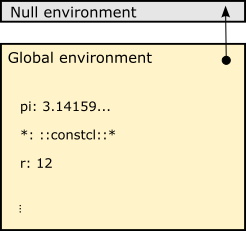
\includegraphics{images/env1.png}
\section{Unfinished code in file environment.ans line 183}
\section{Unfinished code in file environment.ans line 186}
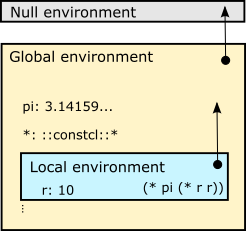
\includegraphics{images/env2.png}
\section{Unfinished code in file environment.ans line 188}
\section{Unfinished code in file environment.ans line 190}
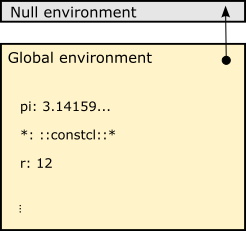
\includegraphics{images/env1.png}

During a call to the procedure \texttt{circle-area}, the symbol \texttt{r} is bound to the value 10. But we don't want the binding to go into the global environment, possibly clobbering an earlier definition of \texttt{r}. The solution is to use separate (but linked) environments, making \texttt{r}'s binding a local variable\footnote{See \texttt{https://en.wikipedia.org/wiki/Local\_variable}}\index{local variable} in its own environment, which the procedure will be evaluated in. The symbols \texttt{*} and \texttt{pi} will still be available through the local environment's link to the outer global environment. This is all part of lexical scoping\footnote{See \texttt{https://en.wikipedia.org/wiki/Scope\_(computer\_science)\#Lexical\_scope}}\index{lexical scope}. In the first image, we see the global environment before we call \texttt{circle-area} (and also the empty null environment which the global environment links to): During the call. Note how the global \texttt{r} is shadowed by the local one, and how the local environment links to the global one to find \texttt{*} and \texttt{pi}. After the call, we are back to the first state again.

\section{Unfinished code in file environment.ans line 193}
\chapter{Initialization}
\label{initialization}
\section{Unfinished code in file setup.ans line 4}


Initialize the memory space for vector contents.

\section{Unfinished code in file setup.ans line 8}
\begin{lstlisting}
set ::constcl::vectorSpace [lrepeat 1024 #NIL]
\section{Unfinished code in file setup.ans line 11}
set ::constcl::vectorAssign 0
\section{Unfinished code in file setup.ans line 13}
proc ::constcl::vsAlloc {num} {
  # TODO calculate free space
  set va $::constcl::vectorAssign
  incr ::constcl::vectorAssign $num
  return $va
}
\end{lstlisting}
\section{Unfinished code in file setup.ans line 21}


Initialize the symbol table and gensym number.

\section{Unfinished code in file setup.ans line 25}
\begin{lstlisting}
unset -nocomplain ::constcl::symbolTable
set ::constcl::symbolTable [dict create]
\section{Unfinished code in file setup.ans line 29}
set ::constcl::gensymnum 0
\end{lstlisting}
\section{Unfinished code in file setup.ans line 32}


Pre-make a set of constants (e.g. \#NIL, \#t, and \#f) and give them aliases for use in source text.

\section{Unfinished code in file setup.ans line 37}
\begin{lstlisting}
interp alias {} #NIL {} [::constcl::NIL new]
\section{Unfinished code in file setup.ans line 40}
interp alias {} #t {} [::constcl::MkBoolean #t]
\section{Unfinished code in file setup.ans line 42}
interp alias {} #f {} [::constcl::MkBoolean #f]
\section{Unfinished code in file setup.ans line 44}
interp alias {} #-1 {} [N -1]
\section{Unfinished code in file setup.ans line 46}
interp alias {} #0 {} [N 0]
\section{Unfinished code in file setup.ans line 48}
interp alias {} #1 {} [N 1]
\section{Unfinished code in file setup.ans line 50}
interp alias {} #+ {} [::constcl::MkSymbol +]
\section{Unfinished code in file setup.ans line 52}
interp alias {} #- {} [::constcl::MkSymbol -]
\section{Unfinished code in file setup.ans line 54}
interp alias {} #UNS {} [::constcl::Unspecified new]
\section{Unfinished code in file setup.ans line 56}
interp alias {} #UND {} [::constcl::Undefined new]
\section{Unfinished code in file setup.ans line 58}
interp alias {} #EOF {} [::constcl::EndOfFile new]
\end{lstlisting}
\section{Unfinished code in file setup.ans line 61}


Initialize the definition register with the queen of numbers (or at least a double-precision floating point approximation).

\section{Unfinished code in file setup.ans line 66}
\index{pi}
\begin{lstlisting}
dict set ::constcl::defreg pi [N 3.1415926535897931]
\end{lstlisting}
\section{Unfinished code in file setup.ans line 71}


In this interpreter, \texttt{nil} does refer to the empty list.

\section{Unfinished code in file setup.ans line 75}
\index{nil}
\begin{lstlisting}
reg nil #NIL
\end{lstlisting}
\section{Unfinished code in file setup.ans line 80}
\section{Unfinished code in file setup.ans line 81}
\section{Environment startup}
\label{environment-startup}
\index{Environment startup}
\section{Unfinished code in file setup.ans line 83}

\section{Unfinished code in file setup.ans line 88}

On startup, two \texttt{Environment} objects called \texttt{null\_env} (the null environment, not the same as \texttt{null-environment} in Scheme) and \texttt{global\_env} (the global environment) are created. Make \texttt{null\_env} empty and judgemental: this is where searches for unbound symbols end up.

\section{Unfinished code in file setup.ans line 92}
\index{null\_env}
\begin{lstlisting}
::constcl::Environment create \
  ::constcl::null_env #NIL {}
\section{Unfinished code in file setup.ans line 97}
oo::objdefine ::constcl::null_env {
  method find {sym} {
    self
  }
  method get {sym} {
    ::error "Unbound variable: [$sym name]"
  }
  method set {sym val} {
    ::error "Unbound variable: [$sym name]"
  }
}
\end{lstlisting}
\section{Unfinished code in file setup.ans line 110}


Meanwhile, \texttt{global\_env} is populated with all the definitions from the definitions register, \texttt{defreg}. This is where top level evaluation happens.

\section{Unfinished code in file setup.ans line 115}
\index{global\_env}
\begin{lstlisting}
namespace eval ::constcl {
  set keys [list {*}[lmap key [dict keys $defreg] {
    S $key
  }]]
  set vals [dict values $defreg]
  Environment create global_env $keys $vals \
    ::constcl::null_env
}
\end{lstlisting}
\section{Unfinished code in file setup.ans line 127}


Load the Scheme base to add more definitions to the global environment.

\section{Unfinished code in file setup.ans line 131}
\index{schemebase}
\begin{lstlisting}
pe {(load "schemebase.scm")}
\end{lstlisting}
\section{Unfinished code in file setup.ans line 136}


Thereafter, each time a user-defined procedure is called, a new \texttt{Environment} object is created to hold the bindings introduced by the call, and also a link to the outer environment (the one closed over when the procedure was defined).

\section{Unfinished code in file setup.ans line 142}
\section{Unfinished code in file setup.ans line 143}
\section{Unfinished code in file setup.ans line 149}
\section{Unfinished code in file setup.ans line 154}
\section{Unfinished code in file setup.ans line 159}
\section{Unfinished code in file setup.ans line 165}
\section{Unfinished code in file setup.ans line 170}
\section{Unfinished code in file setup.ans line 174}
\section{Unfinished code in file setup.ans line 178}
\section{Unfinished code in file setup.ans line 183}
\section{Unfinished code in file setup.ans line 187}
\section{Unfinished code in file setup.ans line 191}
\section{Unfinished code in file setup.ans line 196}
\section{Unfinished code in file setup.ans line 201}
\section{Unfinished code in file setup.ans line 205}
\section{Unfinished code in file setup.ans line 209}
\section{Unfinished code in file setup.ans line 213}
\section{Unfinished code in file setup.ans line 219}
\section{Unfinished code in file setup.ans line 223}
\section{Unfinished code in file setup.ans line 227}
\section{Unfinished code in file setup.ans line 231}
\section{Unfinished code in file setup.ans line 235}
\section{Unfinished code in file setup.ans line 239}
\section{Unfinished code in file setup.ans line 243}
\section{Unfinished code in file setup.ans line 247}
\section{Unfinished code in file setup.ans line 252}
\section{Unfinished code in file setup.ans line 256}
\section{Unfinished code in file setup.ans line 260}
\section{Unfinished code in file setup.ans line 264}
\section{Unfinished code in file setup.ans line 268}
\section{Unfinished code in file setup.ans line 275}
\section{Unfinished code in file setup.ans line 283}
\section{Unfinished code in file setup.ans line 287}
\section{Unfinished code in file setup.ans line 300}
\section{Unfinished code in file setup.ans line 315}
\section{Unfinished code in file setup.ans line 326}
\section{Unfinished code in file setup.ans line 340}
\section{Unfinished code in file setup.ans line 361}
\section{Unfinished code in file setup.ans line 363}
\section{Unfinished code in file repl.ans line 3}
\chapter{The REPL}
\label{the-repl}
\section{Unfinished code in file repl.ans line 5}


The REPL (read-eval-print loop) is a loop that repeatedly \emph{reads} a Scheme source string from the user through the command \texttt{::constcl::input} (breaking the loop if given an empty line) and \texttt{::constcl::parse}, \emph{evaluates} it using \texttt{::constcl::eval}, and \emph{prints} using \texttt{::constcl::write}.

\section{Unfinished code in file repl.ans line 13}

\section{Unfinished code in file repl.ans line 16}

\textbf{input} \texttt{input} is modelled after the Python 3 function. It displays a prompt and reads a string.

\section{Unfinished code in file repl.ans line 19}
\index{input}
\begin{lstlisting}
proc ::constcl::input {prompt} {
  puts -nonewline $prompt
  flush stdout
  set buf [gets stdin]
  set openpars [regexp -all -inline {\(} $buf]
  set clsepars [regexp -all -inline {\)} $buf]
  set openbrak [regexp -all -inline {\[} $buf]
  set clsebrak [regexp -all -inline {\]} $buf]
  while {[llength $openpars] > [llength $clsepars] ||
         [llength $openbrak] > [llength $clsebrak]} {
    ::append buf [gets stdin]
    set openpars [regexp -all -inline {\(} $buf]
    set clsepars [regexp -all -inline {\)} $buf]
    set openbrak [regexp -all -inline {\[} $buf]
    set clsebrak [regexp -all -inline {\]} $buf]
  }
  return $buf
}
\end{lstlisting}
\section{Unfinished code in file repl.ans line 41}

\section{Unfinished code in file repl.ans line 44}

\textbf{repl} \texttt{repl} puts the 'loop' in the read-eval-print loop. It repeats prompting for a string until given a blank input. Given non-blank input, it parses and evaluates the string, printing the resulting value.

\section{Unfinished code in file repl.ans line 49}
\index{repl}
\begin{lstlisting}
proc ::repl {{prompt "ConsTcl> "}} {
  set cur_env [
    ::constcl::Environment new #NIL {} \
      ::constcl::global_env]
  set str [::constcl::input $prompt]
  while {$str ne ""} {
    set expr [::constcl::parse $str]
    set val [::constcl::eval $expr $cur_env]
    ::constcl::write $val
    set str [::constcl::input $prompt]
  }
  $cur_env destroy
}
\end{lstlisting}
\section{Unfinished code in file repl.ans line 66}
\section{Unfinished code in file schemebase.ans line 3}
\chapter{A Scheme base}
\label{a-scheme-base}
\section{Unfinished code in file schemebase.ans line 5}
\begin{lstlisting}
; An assortment of procedures to supplement the builtins.
\end{lstlisting}
\section{Unfinished code in file schemebase.ans line 9}
\section{Lookup table procedures}
\label{lookup-table-procedures}
\index{Lookup table procedures}
\section{Unfinished code in file schemebase.ans line 11}
\subsection{get procedure}
\label{get-procedure}
\index{get procedure}
\section{Unfinished code in file schemebase.ans line 13}


\texttt{get} is a procedure for picking out values out of property lists. It returns either the value or \texttt{\#f} if the key isn't found.

\section{Unfinished code in file schemebase.ans line 18}
\noindent\begin{tabular}{ |p{1.9cm} p{8cm}| }
\hline
\rowcolor[HTML]{CCCCCC} \multicolumn{2}{|l|}{\bf get (public)} \\
plist & a Lisp list of Lisp values \\
key & a symbol \\
\textit{Returns:} & a Lisp value OR \#f \\
\hline
\end{tabular}
\section{Unfinished code in file schemebase.ans line 22}
\begin{lstlisting}
(define (get plist key)
  (let ((v (memq key plist)))
    (if v
      (cadr v)
      #f)))
\end{lstlisting}
\section{Unfinished code in file schemebase.ans line 30}
\subsection{list-find-key procedure}
\label{list-find-key-procedure}
\index{list-find-key procedure}
\section{Unfinished code in file schemebase.ans line 32}


\texttt{list-find-key} searches for a key in a property list. If it finds it, it returns the (0-based) index of it. If it doesn't find it, it returns -1. It doesn't look at the values.

\section{Unfinished code in file schemebase.ans line 38}
\noindent\begin{tabular}{ |p{1.9cm} p{8cm}| }
\hline
\rowcolor[HTML]{CCCCCC} \multicolumn{2}{|l|}{\bf list-find-key (public)} \\
lst & a Lisp list of Lisp values \\
key & a symbol \\
\textit{Returns:} & a number \\
\hline
\end{tabular}
\section{Unfinished code in file schemebase.ans line 42}
\begin{lstlisting}
(define (list-find-key lst key)
  (lfk lst key 0))
\end{lstlisting}
\section{Unfinished code in file schemebase.ans line 47}
\subsection{lfk procedure}
\label{lfk-procedure}
\index{lfk procedure}
\section{Unfinished code in file schemebase.ans line 49}


\texttt{lfk} does the work for \texttt{list-find-key}.

\section{Unfinished code in file schemebase.ans line 53}
\noindent\begin{tabular}{ |p{1.9cm} p{8cm}| }
\hline
\rowcolor[HTML]{CCCCCC} \multicolumn{2}{|l|}{\bf lfk (public)} \\
lst & a Lisp list of Lisp values \\
key & a symbol \\
count & a number \\
\textit{Returns:} & a number \\
\hline
\end{tabular}
\section{Unfinished code in file schemebase.ans line 57}
\begin{lstlisting}
(define (lfk lst key count)
  (if (null? lst)
    -1
    (if (eq? (car lst) key)
      count
      (lfk (cddr lst) key (+ count 2)))))
\end{lstlisting}
\section{Unfinished code in file schemebase.ans line 66}
\subsection{list-set! procedure}
\label{list-set"!-procedure}
\index{list-set"! procedure}
\section{Unfinished code in file schemebase.ans line 68}


\texttt{list-set!} works in analogy with \texttt{string-set!}. Given a list and an index, it finds the place to insert a value. Is in real trouble if the index value is out of range.

\section{Unfinished code in file schemebase.ans line 74}
\noindent\begin{tabular}{ |p{1.9cm} p{8cm}| }
\hline
\rowcolor[HTML]{CCCCCC} \multicolumn{2}{|l|}{\bf list-set! (public)} \\
lst & a Lisp list of Lisp values \\
idx & a number \\
val & a Lisp value \\
\textit{Returns:} & a Lisp value \\
\hline
\end{tabular}
\section{Unfinished code in file schemebase.ans line 78}
\begin{lstlisting}
(define (list-set! lst idx val)
  (if (zero? idx)
    (set-car! lst val)
    (list-set! (cdr lst) (- idx 1) val)))
\end{lstlisting}
\section{Unfinished code in file schemebase.ans line 85}
\subsection{delete! procedure}
\label{delete"!-procedure}
\index{delete"! procedure}
\section{Unfinished code in file schemebase.ans line 87}


\texttt{delete!} removes a key-value pair from a property list. Returns the list.

\section{Unfinished code in file schemebase.ans line 91}
\noindent\begin{tabular}{ |p{1.9cm} p{8cm}| }
\hline
\rowcolor[HTML]{CCCCCC} \multicolumn{2}{|l|}{\bf delete! (public)} \\
lst & a Lisp list of Lisp values \\
key & a symbol \\
\textit{Returns:} & a Lisp list of Lisp values \\
\hline
\end{tabular}
\section{Unfinished code in file schemebase.ans line 95}
\begin{lstlisting}
(define (delete! lst key)
  (let ((idx (list-find-key lst key)))
    (if (< idx 0)
      lst
      (if (= idx 0)
        (set! lst (cddr lst))
        (let ((bef (del-seek lst (- idx 1)))
              (aft (del-seek lst (+ idx 2))))
          (set-cdr! bef aft))))
    lst))
\end{lstlisting}
\section{Unfinished code in file schemebase.ans line 108}
\subsection{del-seek procedure}
\label{del-seek-procedure}
\index{del-seek procedure}
\section{Unfinished code in file schemebase.ans line 110}


\texttt{del-seek} does the searching for \texttt{delete!}.

\section{Unfinished code in file schemebase.ans line 114}
\noindent\begin{tabular}{ |p{1.9cm} p{8cm}| }
\hline
\rowcolor[HTML]{CCCCCC} \multicolumn{2}{|l|}{\bf del-seek (public)} \\
lst & a Lisp list of Lisp values \\
idx & a number \\
\textit{Returns:} & a Lisp list of Lisp values \\
\hline
\end{tabular}
\section{Unfinished code in file schemebase.ans line 118}
\begin{lstlisting}
(define (del-seek lst idx)
  (if (zero? idx)
    lst
    (del-seek (cdr lst) (- idx 1))))
\end{lstlisting}
\section{Unfinished code in file schemebase.ans line 125}
\subsection{get-alist procedure}
\label{get-alist-procedure}
\index{get-alist procedure}
\section{Unfinished code in file schemebase.ans line 127}


\texttt{get-alist} is like \texttt{get} but for association lists.

\section{Unfinished code in file schemebase.ans line 131}
\noindent\begin{tabular}{ |p{1.9cm} p{8cm}| }
\hline
\rowcolor[HTML]{CCCCCC} \multicolumn{2}{|l|}{\bf get-alist (public)} \\
lst & a Lisp list of association pairs \\
key & a symbol \\
\textit{Returns:} & a Lisp value \\
\hline
\end{tabular}
\section{Unfinished code in file schemebase.ans line 135}
\begin{lstlisting}
(define (get-alist lst key)
  (let ((item (assq key lst)))
    (if item
      (cdr item)
      #f)))
\end{lstlisting}
\section{Unfinished code in file schemebase.ans line 143}
\subsection{pairlis procedure}
\label{pairlis-procedure}
\index{pairlis procedure}
\section{Unfinished code in file schemebase.ans line 145}


\texttt{pairlis} takes two lists like \texttt{'(a b c)} and \texttt{'(1 2 3)} and produces a list of association pairs \texttt{'((a . 1) (b . 2) (c . 3))}.

\section{Unfinished code in file schemebase.ans line 150}
\noindent\begin{tabular}{ |p{1.9cm} p{8cm}| }
\hline
\rowcolor[HTML]{CCCCCC} \multicolumn{2}{|l|}{\bf pairlis (public)} \\
a & a Lisp list of Lisp values \\
b & a Lisp list of Lisp values \\
\textit{Returns:} & a Lisp list of association pairs \\
\hline
\end{tabular}
\section{Unfinished code in file schemebase.ans line 154}
\begin{lstlisting}
(define (pairlis a b)
  (if (null? a)
    ()
    (cons
      (cons (car a) (car b))
      (pairlis (cdr a) (cdr b)))))
\end{lstlisting}
\section{Unfinished code in file schemebase.ans line 163}
\subsection{set-alist! procedure}
\label{set-alist"!-procedure}
\index{set-alist"! procedure}
\section{Unfinished code in file schemebase.ans line 165}


\texttt{set-alist!} updates a value in an association list, given a key.

\section{Unfinished code in file schemebase.ans line 169}
\noindent\begin{tabular}{ |p{1.9cm} p{8cm}| }
\hline
\rowcolor[HTML]{CCCCCC} \multicolumn{2}{|l|}{\bf set-alist! (public)} \\
lst & a Lisp list of association pairs \\
key & a symbol \\
val & a Lisp value \\
\textit{Returns:} & a Lisp list of association pairs \\
\hline
\end{tabular}
\section{Unfinished code in file schemebase.ans line 173}
\begin{lstlisting}
(define (set-alist! lst key val)
  (let ((item (assq key lst)))
    (if item
      (begin (set-cdr! item val) lst)
      lst)))
\end{lstlisting}
\section{Unfinished code in file schemebase.ans line 181}
\section{Other}
\label{other}
\index{Other}
\section{Unfinished code in file schemebase.ans line 183}
\subsection{fact procedure}
\label{fact-procedure}
\index{fact procedure}
\section{Unfinished code in file schemebase.ans line 185}


\texttt{fact} calculates the factorial of \emph{n}.

\section{Unfinished code in file schemebase.ans line 189}
\noindent\begin{tabular}{ |p{1.9cm} p{8cm}| }
\hline
\rowcolor[HTML]{CCCCCC} \multicolumn{2}{|l|}{\bf fact (public)} \\
n & a number \\
\textit{Returns:} & a number \\
\hline
\end{tabular}
\section{Unfinished code in file schemebase.ans line 193}
\begin{lstlisting}
(define (fact n)
  (if (<= n 1)
    1
    (* n (fact (- n 1)))))
\end{lstlisting}

\printindex
\end{document}

